% Template adapted from https://github.com/jgm/pandoc-templates/blob/master/default.latex
% To be used with XeLaTex in memoiR
%%%%%%%%%%%%%%%%%%%%%%%%%%%%%%%%%%%%%%%%%%%%%%%%%%%%%%%%%%%%%%%%%%%%%%%%%%%%%%%%%%%%%%%%%

% Options for packages loaded elsewhere
\PassOptionsToPackage{unicode=true}{hyperref}
\PassOptionsToPackage{hyphens}{url}
\PassOptionsToPackage{dvipsnames,svgnames*,x11names*}{xcolor}
% Right to left support


\documentclass[
  12pt,
  american,
  a4paper,
  extrafontsizes,onecolumn,openright
  ]{memoir}

% Double (or whatever) spacing

% Math
\usepackage{amssymb, amsmath}
% mathspec: arbitrary math fonts
\usepackage{unicode-math}
\defaultfontfeatures{Scale=MatchLowercase}
\defaultfontfeatures[\rmfamily]{Ligatures=TeX,Scale=1}

% Fonts
\usepackage{lmodern}
\usepackage{fontspec}
% Main font
\setmainfont[Extension=.otf,UprightFont=*-regular,BoldFont=*-bold,BoldItalicFont=*-bolditalic,ItalicFont=*-italic]{texgyretermes}
% Specific sanserif font
% Specific monotype font
% Specific math font
  \setmathfont[]{texgyretermes-math.otf}
  % Chinese, Japanese, Corean fonts

% Use upquote for straight quotes in verbatim environments
\usepackage{upquote}
% Use microtype
\usepackage[]{microtype}
\UseMicrotypeSet[protrusion]{basicmath} % disable protrusion for tt fonts

% Verbatim in note

% Color links
\usepackage{xcolor}

% Strikeout

% Necessary for code chunks
\usepackage{color}
\usepackage{fancyvrb}
\newcommand{\VerbBar}{|}
\newcommand{\VERB}{\Verb[commandchars=\\\{\}]}
\DefineVerbatimEnvironment{Highlighting}{Verbatim}{commandchars=\\\{\}}
% Add ',fontsize=\small' for more characters per line
\usepackage{framed}
\definecolor{shadecolor}{RGB}{248,248,248}
\newenvironment{Shaded}{\begin{snugshade}}{\end{snugshade}}
\newcommand{\AlertTok}[1]{\textcolor[rgb]{0.94,0.16,0.16}{#1}}
\newcommand{\AnnotationTok}[1]{\textcolor[rgb]{0.56,0.35,0.01}{\textbf{\textit{#1}}}}
\newcommand{\AttributeTok}[1]{\textcolor[rgb]{0.13,0.29,0.53}{#1}}
\newcommand{\BaseNTok}[1]{\textcolor[rgb]{0.00,0.00,0.81}{#1}}
\newcommand{\BuiltInTok}[1]{#1}
\newcommand{\CharTok}[1]{\textcolor[rgb]{0.31,0.60,0.02}{#1}}
\newcommand{\CommentTok}[1]{\textcolor[rgb]{0.56,0.35,0.01}{\textit{#1}}}
\newcommand{\CommentVarTok}[1]{\textcolor[rgb]{0.56,0.35,0.01}{\textbf{\textit{#1}}}}
\newcommand{\ConstantTok}[1]{\textcolor[rgb]{0.56,0.35,0.01}{#1}}
\newcommand{\ControlFlowTok}[1]{\textcolor[rgb]{0.13,0.29,0.53}{\textbf{#1}}}
\newcommand{\DataTypeTok}[1]{\textcolor[rgb]{0.13,0.29,0.53}{#1}}
\newcommand{\DecValTok}[1]{\textcolor[rgb]{0.00,0.00,0.81}{#1}}
\newcommand{\DocumentationTok}[1]{\textcolor[rgb]{0.56,0.35,0.01}{\textbf{\textit{#1}}}}
\newcommand{\ErrorTok}[1]{\textcolor[rgb]{0.64,0.00,0.00}{\textbf{#1}}}
\newcommand{\ExtensionTok}[1]{#1}
\newcommand{\FloatTok}[1]{\textcolor[rgb]{0.00,0.00,0.81}{#1}}
\newcommand{\FunctionTok}[1]{\textcolor[rgb]{0.13,0.29,0.53}{\textbf{#1}}}
\newcommand{\ImportTok}[1]{#1}
\newcommand{\InformationTok}[1]{\textcolor[rgb]{0.56,0.35,0.01}{\textbf{\textit{#1}}}}
\newcommand{\KeywordTok}[1]{\textcolor[rgb]{0.13,0.29,0.53}{\textbf{#1}}}
\newcommand{\NormalTok}[1]{#1}
\newcommand{\OperatorTok}[1]{\textcolor[rgb]{0.81,0.36,0.00}{\textbf{#1}}}
\newcommand{\OtherTok}[1]{\textcolor[rgb]{0.56,0.35,0.01}{#1}}
\newcommand{\PreprocessorTok}[1]{\textcolor[rgb]{0.56,0.35,0.01}{\textit{#1}}}
\newcommand{\RegionMarkerTok}[1]{#1}
\newcommand{\SpecialCharTok}[1]{\textcolor[rgb]{0.81,0.36,0.00}{\textbf{#1}}}
\newcommand{\SpecialStringTok}[1]{\textcolor[rgb]{0.31,0.60,0.02}{#1}}
\newcommand{\StringTok}[1]{\textcolor[rgb]{0.31,0.60,0.02}{#1}}
\newcommand{\VariableTok}[1]{\textcolor[rgb]{0.00,0.00,0.00}{#1}}
\newcommand{\VerbatimStringTok}[1]{\textcolor[rgb]{0.31,0.60,0.02}{#1}}
\newcommand{\WarningTok}[1]{\textcolor[rgb]{0.56,0.35,0.01}{\textbf{\textit{#1}}}}

% Listings package

% Tables
\usepackage{longtable,booktabs,tabu}
% Fix footnotes in tables (requires footnote package)
\IfFileExists{footnote.sty}{\usepackage{footnote}\makesavenoteenv{longtable}}{}

% Graphics
\usepackage{graphicx,grffile}
\graphicspath{{images/}}
\makeatletter
\def\maxwidth{\ifdim\Gin@nat@width>\linewidth\linewidth\else\Gin@nat@width\fi}
\def\maxheight{\ifdim\Gin@nat@height>\textheight\textheight\else\Gin@nat@height\fi}
\makeatother
% Scale images if necessary, so that they will not overflow the page
% margins by default, and it is still possible to overwrite the defaults
% using explicit options in \includegraphics[width, height, ...]{}
\setkeys{Gin}{width=\maxwidth,height=\maxheight,keepaspectratio}

% Prevent overfull lines
\setlength{\emergencystretch}{3em}  
\providecommand{\tightlist}{%
  \setlength{\itemsep}{0pt}\setlength{\parskip}{0pt}}

% Number sections for memoir (secnumdepth counter is ignored)
\setsecnumdepth{subsection}

% Set default figure placement to htbp
\makeatletter
\def\fps@figure{htbp}
\makeatother

% Spacing in lists
\usepackage{enumitem}

% Polyglossia
\usepackage{polyglossia}
\setmainlanguage{en-US}

% localized quotes
\usepackage[strict,autostyle]{csquotes}
\MakeOuterQuote{"}

% BibLaTeX
\usepackage[backend=biber,style=authoryear-ibid,isbn=false,backref=true,giveninits=true,uniquename=init,maxcitenames=2,maxbibnames=150,sorting=nyt,sortcites=false]{biblatex}
\addbibresource{references.bib}

% cslreferences environment required by pandoc > 2.7



%%%%%%%%%%%%%%%%%%%%%%%%%%%%%%%%%%%%%%%%%%%%%%%%%%%%%%%%%%
% memoiR format

% Chapter Summary environment 
\usepackage[tikz]{bclogo}
\newenvironment{Summary}
  {\begin{bclogo}[logo=\bctrombone, noborder=true, couleur=lightgray!50]{L'essentiel}\parindent0pt}
  {\end{bclogo}}
% Syntax:
%
%```{block, type='Summary'}
% Deliver message here.
% ```

% scriptsize code 
\let\oldverbatim\verbatim
\def\verbatim{\oldverbatim\scriptsize}
% Applies to code blocks and R code results
% code chunk options size='scriptsize' applies only to R code and results
% if the code chunk sets a different size, \def\verbatim{...} is prioritary for code results 


% memoiR dalef3 chapter style 
% https://ctan.crest.fr/tex-archive/info/latex-samples/MemoirChapStyles/MemoirChapStyles.pdf
\usepackage{soul}
\definecolor{nicered}{rgb}{.647,.129,.149}
\makeatletter
\newlength\dlf@normtxtw
\setlength\dlf@normtxtw{\textwidth}
\def\myhelvetfont{\def\sfdefault{mdput}}
\newsavebox{\feline@chapter}
\newcommand\feline@chapter@marker[1][4cm]{%
  \sbox\feline@chapter{%
    \resizebox{!}{#1}{\fboxsep=1pt%
	  \colorbox{nicered}{\color{white}\bfseries\sffamily\thechapter}%
	}}%
  \rotatebox{90}{%
    \resizebox{%
	  \heightof{\usebox{\feline@chapter}}+\depthof{\usebox{\feline@chapter}}}%
	{!}{\scshape\so\@chapapp}}\quad%
  \raisebox{\depthof{\usebox{\feline@chapter}}}{\usebox{\feline@chapter}}%
 }
\newcommand\feline@chm[1][4cm]{%
  \sbox\feline@chapter{\feline@chapter@marker[#1]}%
  \makebox[0pt][l]{% aka \rlap
    \makebox[1cm][r]{\usebox\feline@chapter}%
  }}
\makechapterstyle{daleif1}{
  \renewcommand\chapnamefont{\normalfont\Large\scshape\raggedleft\so}
  \renewcommand\chaptitlefont{\normalfont\huge\bfseries\scshape\color{nicered}}
  \renewcommand\chapternamenum{}
  \renewcommand\printchaptername{}
  \renewcommand\printchapternum{\null\hfill\feline@chm[2.5cm]\par}
  \renewcommand\afterchapternum{\par\vskip\midchapskip}
  \renewcommand\printchaptertitle[1]{\chaptitlefont\raggedleft ##1\par}
}
\makeatother


% Layout
%%%%%%%%%%%%%%%%%%%%%%%%%%%%%%%%%%%%%%%%%%%%%%%%%%%%%%%%%%

% Based on memoir, style companion
\newcommand{\MemoirChapStyle}{daleif1}
\newcommand{\MemoirPageStyle}{Ruled}

% Space between paragraphs
\usepackage{parskip}
  \abnormalparskip{3pt}

% Adjust margin paragraphs vertical position
\usepackage{marginfix}


% Margins
%%%%%%%%%%%%%%%%%%%%%%%%%%%%%%%%%%%%%%%

% allow use of '-',+','/' ans '*' to make simple length computation
\usepackage{calc}

% Full-width figures utilities
\newlength\widthw % full width
\newlength{\rf}
\newcommand*{\definesHSpace}{
  \strictpagecheck % slower but efficient detection of odd/even pages
  \checkoddpage
  \ifoddpage
  \setlength{\rf}{0mm}
  \else
  \setlength{\rf}{\marginparsep+\marginparwidth}
  \fi
}

\makeatletter
% 1" margins for the front matter.
\newcommand*{\SmallMargins}{
  \setlrmarginsandblock{1.5in}{1.5in}{*}
  \setmarginnotes{0.1in}{0.1in}{0.1in}
 \setulmarginsandblock{1.5in}{1in}{*}
  \checkandfixthelayout
  \ch@ngetext
  \clearpage
  \setlength{\widthw}{\textwidth+\marginparsep+\marginparwidth}
  \footnotesatfoot
  \chapterstyle{\MemoirChapStyle}  % Chapter and page styles must be recalled
  \pagestyle{\MemoirPageStyle}
}

% 3" outer margin for the main matter
\newcommand{\LargeMargins}{\SmallMargins}
\makeatother

% Figure captions and footnotes in outer margins


% Local toc
%%%%%%%%%%%%%%%%%%%%%%%%%%%%%%%%%%%%%%%%%%%%%%%%%%%%%%%%%%

\usepackage{titletoc}
\newcommand{\toc}[1]{%
  \startcontents[chapters]%
  \printcontents[chapters]{}{1}[#1]{}%
  ~\newline%
}


% Main title page with filigrane
%%%%%%%%%%%%%%%%%%%%%%%%%%%%%%%%%%%%%%%%%%%%%%%%%%%%%%%%%%

% Text blocks
\usepackage[absolute,overlay]{textpos}
  \setlength{\TPHorizModule}{1mm}
  \setlength{\TPVertModule}{1mm}

\newcommand{\MainTitlePage}[2]{
  \SmallMargins % Margins
  \pagestyle{empty} % No header/footer
  \textblockorigin{\stockwidth-\paperwidth-\trimedge}{\trimtop} % recto
  \begin{textblock*}{2mm}(\spinemargin/2,\uppermargin/2)
    \rule{1pt}{\paperheight-\uppermargin}
  \end{textblock*}
  \begin{textblock*}{\paperwidth*2/3}(\paperwidth/5, \paperheight/5)
    \flushright
    \begin{Spacing}{3}
      {\fontfamily{qtm}\selectfont\fontsize{45}{45}\selectfont\textsc{\thetitle}}
    \end{Spacing}
  \end{textblock*}
    \begin{textblock*}{\paperwidth/2}[1, 1](\paperwidth, \paperheight)
    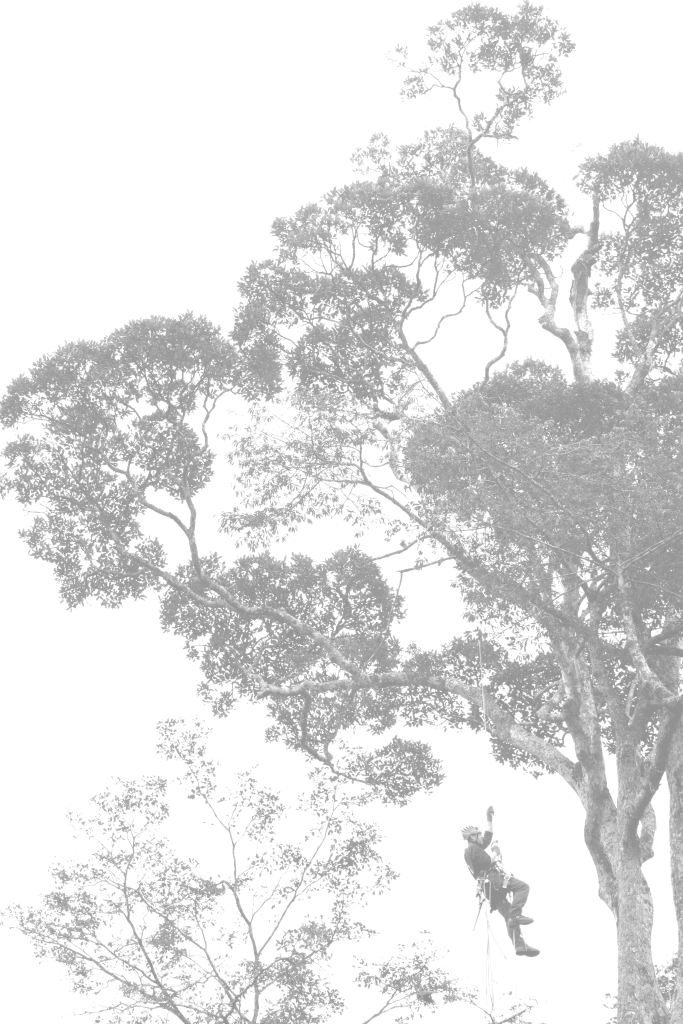
\includegraphics[width=\paperwidth/2]{filigrane}
  \end{textblock*}
  \begin{textblock*}{\paperwidth*2/3}(\spinemargin, \paperheight/2)
    {\fontfamily{qtm}\huge\theauthor}
  \end{textblock*}
    \begin{textblock*}{\paperwidth*2/3}[0, 1](\spinemargin, \uppermargin+\textheight)
    \normalfont\thedate
  \end{textblock*}
  ~\\ % Print a character or the page will not exist
  \newpage
  \textblockorigin{\trimedge}{\trimtop} % verso
  \begin{textblock*}{\textwidth}(\paperwidth-\spinemargin-\textwidth, \uppermargin)
    #1
  \end{textblock*}
  \begin{textblock*}{\textwidth}[0,1](\paperwidth-\spinemargin-\textwidth, \uppermargin+\textheight+\footskip)
    \centering
    
\includegraphics[width=\paperwidth/4]{logo}\\ \bigskip
    #2
  \end{textblock*}
  ~\\ % Print a character or the page will not exist
  \newpage
}

% Clear page and open an even one (\clearpage opens an odd one)
\newcommand{\evenpage}{
  \clearpage
  \strictpagecheck % slower but efficient detection of odd/even pages
  \checkoddpage
  \ifoddpage
    \thispagestyle{empty}
    ~\\ % Print a character or the page will not exist
    \newpage
  \else
    % do nothing
  \fi
}


%% PDF title page to insert
%%%%%%%%%%%%%%%%%%%%%%%%%%%%%%%%%%%%%%%%%%%%%%%%%%%%%%%%%%



%% Bibliography
%%%%%%%%%%%%%%%%%%%%%%%%%%%%%%%%%%%%%%%%%%%%%%%%%%%%%%%%%%

% Repeated citation as author-year-title instead of author-title (modification of footcite:note in verbose-inote.cbx)

%% Table of Contents
%%%%%%%%%%%%%%%%%%%%%%%%%%%%%%%%%%%%%%%%%%%%%%%%%%%%%%%%%%

% fix the typesetting of the part number
\renewcommand\partnumberlinebox[2]{#2\ ---\ }


% Fonts
%%%%%%%%%%%%%%%%%%%%%%%%%%%%%%%%%%%%%%%%%%%%%%%%%%%%%%%%%%


% Hyperref comes last
%%%%%%%%%%%%%%%%%%%%%%%%%%%%%%%%%%%%%%%%%%%%%%%%%%%%%%%%%%

\usepackage{hyperref}
\hypersetup{
  pdftitle={Working with R},
  pdfauthor={Eric Marcon},
  colorlinks=true,
  linkcolor=Maroon,
  citecolor=Blue,
  urlcolor=Blue,
  breaklinks=true}

% Don't use monospace font for urls
\urlstyle{same}


% Title, author, date from YAML to LaTeX
%%%%%%%%%%%%%%%%%%%%%%%%%%%%%%%%%%%%%%%%%%%%%%%%%%%%%%%%%%

\title{Working with R}

\author{Eric Marcon}

\date{03/14/2025}


% Include headers (preamble.tex) here
%%%%%%%%%%%%%%%%%%%%%%%%%%%%%%%%%%%%%%%%%%%%%%%%%%%%%%%%%%

\usepackage{booktabs}
\usepackage{longtable}
\usepackage{array}
\usepackage{multirow}
\usepackage{wrapfig}
\usepackage{float}
\usepackage{colortbl}
\usepackage{pdflscape}
\usepackage{tabu}
\usepackage{threeparttable}
\usepackage{threeparttablex}
\usepackage[normalem]{ulem}
\usepackage{makecell}
\usepackage{xcolor}
\usepackage{fontspec}
\usepackage{multicol}
\usepackage{hhline}
\newlength\Oldarrayrulewidth
\newlength\Oldtabcolsep
\usepackage{hyperref}


% End of preamble
%%%%%%%%%%%%%%%%%%%%%%%%%%%%%%%%%%%%%%%%%%%%%%%%%%%%%%%%%%


\begin{document}
\frontmatter

% Title page
%%%%%%%%%%%%%%%%%%%%%%%%%%%%%%%%%%%%%%%%%%%%%%%%%%%%%%%%%%


\MainTitlePage{This document is made in a dynamic and reproducible way thanks to:

\begin{itemize}
  \item \LaTeX, in its Miktex distribution (\url{http://miktex.org/}) and the memoir class (\url{http://www.ctan.org/pkg/memoir}).
  \item R (\url{http://www.r-project.org/}) and RStudio (\url{http://www.rstudio.com/})
  \item bookdown (\url{http://bookdown.org/}) and memoiR (\url{https://ericmarcon.github.io/memoiR/})
\end{itemize}

Its source code is on GitHub: \url{https://github.com/EricMarcon/WorkingWithR/}.

The continuously updated text can be read at \url{https://ericmarcon.github.io/WorkingWithR/}.}{Cover photograph: Hadrien Lalagüe}


% Before Body
%%%%%%%%%%%%%%%%%%%%%%%%%%%%%%%%%%%%%%%%%%%%%%%%%%%%%%%%%%





% Contents
%%%%%%%%%%%%%%%%%%%%%%%%%%%%%%%%%%%%%%%%%%%%%%%%%%%%%%%%%%

\LargeMargins
{
\hypersetup{linkcolor=}
\setcounter{tocdepth}{2}
\tableofcontents
}


% Body
%%%%%%%%%%%%%%%%%%%%%%%%%%%%%%%%%%%%%%%%%%%%%%%%%%%%%%%%%%

\LargeMargins
\chapter*{Presentation}\label{presentation}
\addcontentsline{toc}{chapter}{Presentation}

\section*{Objectives}\label{objectives}
\addcontentsline{toc}{section}{Objectives}

This document is the support of the course \emph{Working with R}.

It proposes an organization of the work around R and RStudio in order to, beyond statistics, write documents efficiently with R Markdown, in various formats (memos, scientific articles, student theses, books, slideshows), create a web site and online R applications (Shiny), produce packages and use R for teaching.
It complements \emph{Reproducible Research with R and R Studio} \autocite{Gandrud2013} with a more hands-on approach, with ready-to-use solutions.

Optimizing the use of the many tools available is covered in detail: \textbf{rmarkdown}, \textbf{bookdown} and \textbf{blogdown} for writing, \textbf{roxygen2}, \textbf{testthat} and \textbf{pkgdown} for packages, source control with git and GitHub, continuous integration with GitHub Actions and Codecov.
Examples are presented at each step, and the necessary code is provided.

Chapter \ref{chap-logiciels} is dedicated to the installation of the necessary tools: R, git and LaTeX.
Chapter \ref{chap-utiliseR} details some advanced aspects of using R: the different languages, the environments, the performance of the code.
The basic use of R is not covered here: good courses are suggested.
Chapter \ref{chap-git} presents source control with git and GitHub.

Chapter \ref{chap-rediger} shows how to write simple (articles) or complex (books) documents with R Markdown, integrating the data, the code to process them and the text to present them.
Chapter \ref{chap-package} presents a step-by-step method to efficiently create a package.
Chapter \ref{chap-ci} introduces the use of continuous integration to automatically produce documents, verify package code and produce package vignettes.
Chapter \ref{chap-shiny} introduces Shiny to develop R interactive applications.
Finally, chapter \ref{chap-enseigner} introduces the tools for teaching R.

\section*{Conventions}\label{conventions}
\addcontentsline{toc}{section}{Conventions}

Package names are in bold in the text, for example: \textbf{ggplot2}.

The identifier used on GitHub is noted \emph{GitHubID}.
Project names are the same as their GitHub repository, noted \emph{RepoID}.

The sign \texttt{\textbar{}\textgreater{}} in the code of the examples indicates that the rest of the code should be on the same line, but is cut for the formatting of this document.
Its use is limited to YAML configuration files, mostly in chapter \ref{chap-ci}.
In all other cases, the code can be copied directly.

\mainmatter

\chapter{Software}\label{chap-logiciels}

\toc{1}

The central tool is obviously R, but its operation is today difficult to consider without its development environment RStudio.
For source control, git and GitHub are the de facto standards.
The set must be completed by a LaTeX distribution for the production of documents in PDF format.
A bibliographic management tool is essential: Zotero and its extension Better BibTeX are perfectly adapted to the framework presented here.
Finally, other software of more occasional use may be necessary, such as Go.

Their installation and coherent organization are presented in this chapter.

\section{R}\label{r}

\subsection{Installation}\label{installation}

R is included in Linux distributions: the package is named \texttt{r-base}.
It does not contain development tools that are often needed, so it is better to install the \texttt{r-base-dev} package as well.
The version of R is often a bit old.
To get the latest version, you have to use a CRAN mirror as a source for the packages: see the full documentation for Ubuntu\footnote{\url{https://doc.ubuntu-fr.org/r}}.

On Windows or Mac, install R after downloading it from CRAN\footnote{\url{https://cran.r-project.org/}}.

\subsection{Rtools}\label{rtools}

On Mac, the installation of R is sufficient from version 4.0.0.

On Windows, the installation must be completed by the \enquote{Rtools}, which contain the development tools, including those necessary to compile packages containing C++ code.

The path of the Rtools (before version 4.2) must be declared to R, by executing the following command in the RStudio console (adapted to version 4.0 of the Rtools):

\scriptsize

\begin{Shaded}
\begin{Highlighting}[]
\CommentTok{\# Rtools : path declaration, }
\CommentTok{\# requires restarting RStudio}
\FunctionTok{writeLines}\NormalTok{(}
  \StringTok{\textquotesingle{}PATH="$\{RTOOLS40\_HOME\}}\SpecialCharTok{\textbackslash{}\textbackslash{}}\StringTok{usr}\SpecialCharTok{\textbackslash{}\textbackslash{}}\StringTok{bin;$\{PATH\}"\textquotesingle{}}\NormalTok{,}
  \AttributeTok{con =} \StringTok{"\textasciitilde{}/.Renviron"}
\NormalTok{)}
\end{Highlighting}
\end{Shaded}

\normalsize

Since version 4.2, this action is unnecessary.

The Rtools must be completed by some missing utilities, to be installed when the need appears (usually a warning from R that the software is not installed).

Package checking returns a warning if \emph{qpdf}\footnote{\url{https://sourceforge.net/projects/qpdf/}} is not installed.
Download the zip file and paste the entire contents of the \texttt{bin} folder into the \texttt{usr/bin} folder of \texttt{Rtools} (\texttt{C:\textbackslash{}Rtools42\textbackslash{}r\textbackslash{}bin} for version 4.2).

Another warning is returned if \emph{Ghostscript} is not available.
Download and install it\footnote{\url{https://www.ghostscript.com/}}.
Then copy the contents of the \texttt{bin} folder to the \texttt{usr/bin} folder of \texttt{Rtools}.

\subsection{Update}\label{update}

It is recommended to use the latest minor version of R: for example, 4.0.x until the release of version 4.1.
It is mandatory to use the latest version to prepare a package submitted to CRAN.

Important changes occur between major versions (version 4 does not allow to use a package compiled for version 3) but also sometimes between minor versions (a binary data file \texttt{.rda} saved under version 3.3 cannot be read by version 3.6).
It is therefore useful to update R regularly.

Installing a new version does not automatically uninstall older versions, which allows you to use more than one version if necessary (for example, if an old and essential package is no longer available).
In common use, it is preferable to uninstall old versions manually after installing a new one.

\subsection{Libraries}\label{sec:librairies}

R packages are found in two folders:

\begin{itemize}
\tightlist
\item
  the \emph{System Library} contains the packages that come with R: \textbf{base}, \textbf{utils}, \textbf{graphics} for example.
  It is located in a subdirectory of the installation program (\texttt{C:\textbackslash{}Program\ Files\textbackslash{}R-4.1.0\textbackslash{}library} for R version 4.1.0 on Windows 10).
\item
  The \emph{User Library} contains those installed by the user.
  Until version 4.1, it is located in the user's home folder, in a subfolder \texttt{R\textbackslash{}win-library\textbackslash{}4.1\textbackslash{}}).
  Since version 4.2, this folder is in the user's local settings, whose folder location is in the environment variable \texttt{\%LOCALAPPDATA\%}.
\end{itemize}

Until version 4.1, if the user's home folder is backed up (for example, if it is replicated in the cloud by OneDrive on Windows), it is not optimal to place the packages there: the traffic generated by backing them up would be heavy and unnecessary.
In order for packages to be installed automatically in the system library, the user must have the right to write to it.
On Windows, give the computer's user group the \enquote{Modify} permission to the library folder, in addition to the default read permissions.
From version 4.2 onwards, there is no reason to change the default operation: local settings are not saved.

If the user library is selected, you must remember to empty the folder corresponding to the old version of R in case of minor version change.

The location of the libraries is given by the function \texttt{.libPaths()}:

\scriptsize

\begin{Shaded}
\begin{Highlighting}[]
\FunctionTok{.libPaths}\NormalTok{()}
\end{Highlighting}
\end{Shaded}

\begin{verbatim}
## [1] "/Users/runner/work/_temp/Library"                                    
## [2] "/Library/Frameworks/R.framework/Versions/4.4-arm64/Resources/library"
\end{verbatim}

\normalsize

\section{RStudio}\label{rstudio}

RStudio is a graphical interface for R and much more: it is designed to simplify project management, make writing and publishing documents easier and integrate source control for example.

\subsection{Installation}\label{installation-1}

Install the latest version of \emph{RStudio Desktop} from the RStudio website\footnote{\url{https://rstudio.com/products/rstudio/download/}}.

A command is available in the \enquote{Help} menu of RStudio to check for a more recent version to install.

\subsection{File encoding}\label{file-encoding}

The files manipulated in R are mostly text files.
Special characters, especially accents, can be encoded in various ways, but the encoding declaration is not integrated in the files.
The default encoding depends on the operating system, which regularly causes problems with the readability of shared files.
The UTF8 encoding has become the standard because it is universally recognized and supports all alphabets without ambiguity.

The first time you use RStudio, create a new R file (\enquote{File \textgreater{} New File \textgreater{} R Script} menu), save it in UTF8 format (\enquote{File \textgreater{} Save with Encoding\ldots{}}), choose UTF8 in the list of formats and check the box \enquote{Set as default encoding for source files}.
Delete the file after saving it.

New files will be encoded in UTF8 format.
Files encoded in another format will not be displayed correctly: they can be reopened with their original encoding (\enquote{File \textgreater{} Reopen with Encoding\ldots{}}), possibly trying several encodings until they are displayed correctly, and then saved in UTF8 format.

\subsection{Working folder}\label{working-folder}

The default working folder is the user's home folder, called \texttt{\textasciitilde{}} by RStudio:

\scriptsize

\begin{Shaded}
\begin{Highlighting}[]
\FunctionTok{Sys.getenv}\NormalTok{(}\StringTok{"R\_USER"}\NormalTok{)}
\end{Highlighting}
\end{Shaded}

\begin{verbatim}
## [1] ""
\end{verbatim}

\normalsize

\begin{itemize}
\tightlist
\item
  \texttt{My\ Documents} on Windows.
\item
  \texttt{Home} on Mac or Linux.
\end{itemize}

You should always work in subfolders of \texttt{\textasciitilde{}}, for example: \texttt{\textasciitilde{}/Training}.

For \emph{RTools} to work properly, the full name of the working directory must not contain spaces (use underscores \texttt{\_}) or special characters.
The current working directory is obtained by the command \texttt{getwd()}.

\scriptsize

\begin{Shaded}
\begin{Highlighting}[]
\FunctionTok{getwd}\NormalTok{()}
\end{Highlighting}
\end{Shaded}

\normalsize

Using source control (see chapter \ref{chap-git}) creates many working files.
Source-controlled projects should not be located in a folder that is already backed up by another means, such as a OneDrive on Windows, otherwise resources will be used excessively: each change validation generates a backup of the modified files, but also of the control files, which can be very large.

\subsection{Solution chosen}\label{sec:solution-dossiers}

The organization of the work environment is a personal matter, depending on the preferences of each individual.
The organization proposed here is only a possibility, to be adapted to one's own choices, but respecting the constraints mentioned.

On Windows, an optimal organization is as follows:

\begin{itemize}
\tightlist
\item
  In one's personal folder (\texttt{My\ Documents}, \texttt{\textasciitilde{}} for R), an \texttt{R} folder is used for simple projects, without source control.
  The backup of this folder is managed elsewhere.
\item
  A folder outside the home folder is used for source-controlled projects.
  The user must have the right to write to it.
  In the Windows organization, the folder corresponding to these criteria is \texttt{\%LOCALAPPDATA\%}, typically \texttt{C:\textbackslash{}Users\textbackslash{}Name\textbackslash{}AppData}.
  The folder will therefore be \texttt{\%LOCALAPPDATA\%\textbackslash{}RProjects}.
  To create it, run \texttt{md\ \%LOCALAPPDATA\%\textbackslash{}RProjects} in a command prompt.
  Pin this folder to the quick access of the file explorer (figure \ref{fig:R-ProjetsR}): paste \texttt{\%LOCALAPPDATA\%\textbackslash{}RProjects} in the address bar of the file explorer, validate, then right click on \enquote{Quick Access} and pin the folder.
\end{itemize}



\scriptsize

\begin{figure}

{\centering 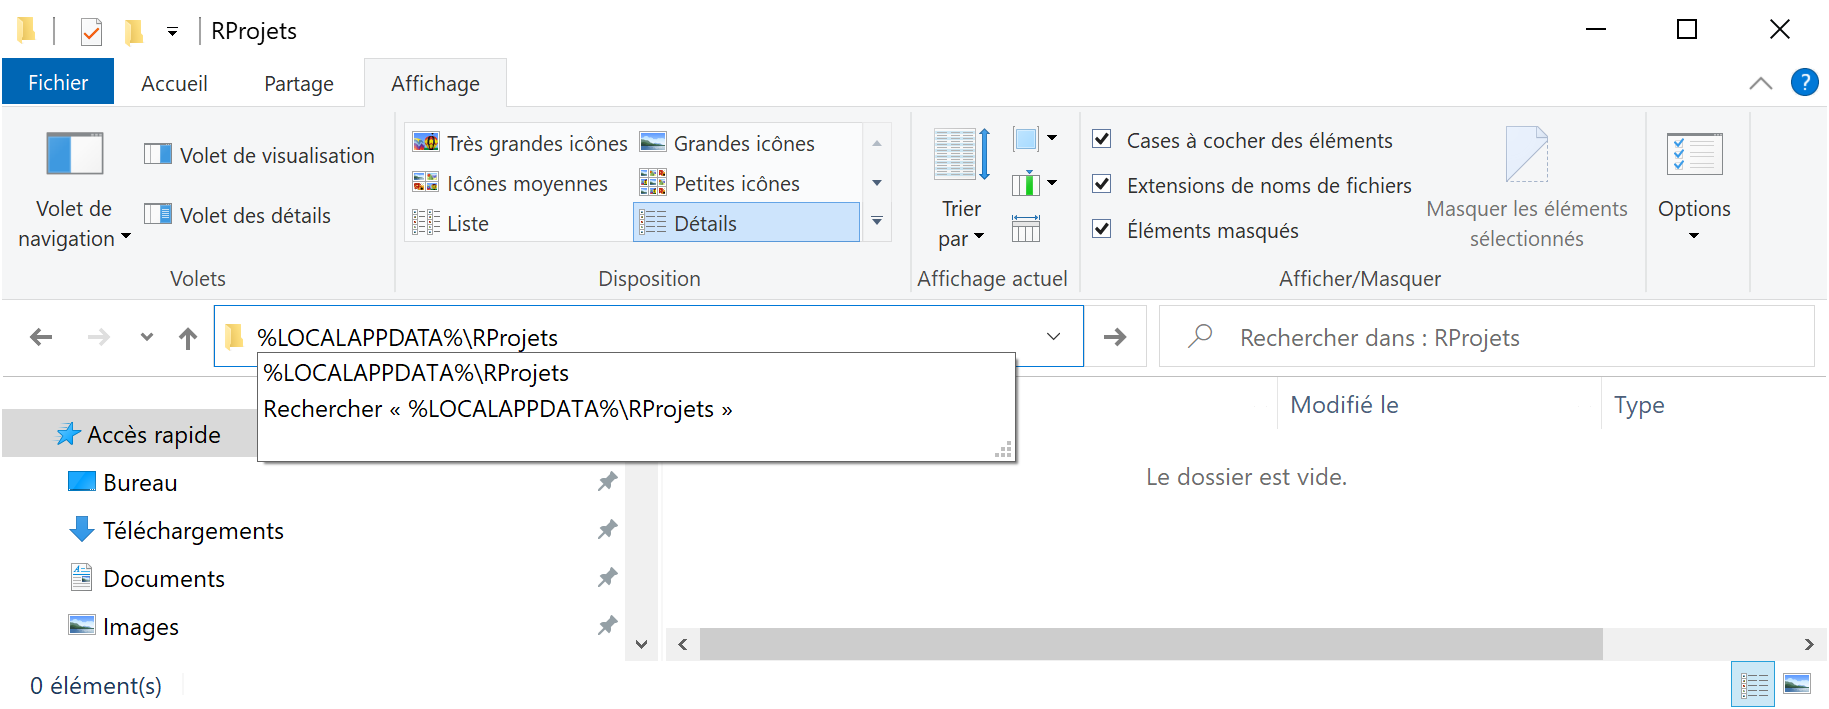
\includegraphics[width=1\linewidth]{images/R-ProjetsR} 

}

\caption{Folder for projects under source control, on Windows.}\label{fig:R-ProjetsR}
\end{figure}

\normalsize

\subsection{Character font}\label{character-font}

The Fira Code\footnote{\url{https://github.com/tonsky/FiraCode}} font provides ligatures: the \enquote{\textless-} characters used for assignment in R, for example, are displayed as an arrow.
To use it in the RStudio editor, simply install it according to the instructions for your operating system and declare it in the global options (\enquote{Tools \textgreater{} Global Options\ldots{}} menu): select \emph{Appearance} and the option \emph{Editor Font}: Fira Code.

\section{Packages}\label{packages}

\subsection{Installation from CRAN}\label{installation-from-cran}

The classic installation of packages uses CRAN.
There is an \enquote{Install} button in the \emph{Packages} window of RStudio.

Packages are uploaded to CRAN by their authors as source code, compressed in a \texttt{.tar.gz} file.
They are available for download as soon as they are validated.
They must then be put in binary format for Windows (in a `.zip' file), which takes some time.

When asked to install a package on Windows, CRAN proposes the source version rather than the binary version if it is more recent (figure \ref{fig:R-BinaryPkg}).



\scriptsize

\begin{figure}

{\centering 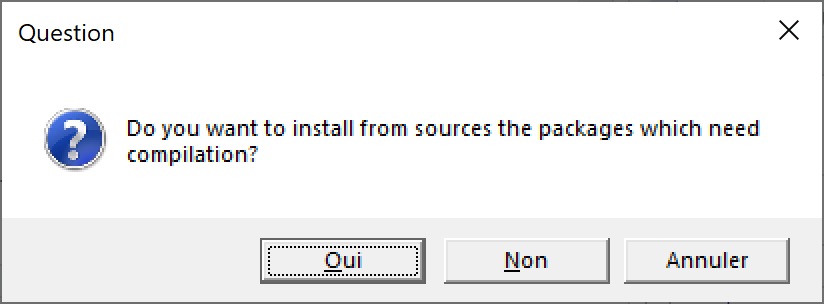
\includegraphics[width=0.8\linewidth]{images/R-BinaryPkg} 

}

\caption{Choice of the version of the packages to install.}\label{fig:R-BinaryPkg}
\end{figure}

\normalsize

The list of packages concerned is displayed in the console, for example:

\begin{verbatim}
  There are binary versions available but the source 
  versions are later:
              binary   source needs_compilation
boot          1.3-24   1.3-25             FALSE
class         7.3-16   7.3-17              TRUE
\end{verbatim}

Some packages require compilation (column \texttt{needs\_compilation}), usually because they contain C++ code.
They can only be installed by \emph{Rtools}.

The installation of packages in source version is much longer than in binary version.
Unless a specific version of a package is needed, it is better to refuse the installation of source versions.

Packages can be updated a little later, after they have been compiled by CRAN.

The \enquote{Update} button in the RStudio \emph{Packages} window allows you to update all installed packages.

\subsection{Installation from GitHub}\label{installation-from-github}

Some packages are not available on CRAN but only on GitHub because they are still under development or because they are not intended to be widely used by the R user community.
It can also be useful to install a development version of a package published on CRAN for a specific use like testing new features.

The installation is handled by the \textbf{remotes} package.
The \texttt{build\_vignettes} argument is needed to create the vignettes of the package.

\scriptsize

\begin{Shaded}
\begin{Highlighting}[]
\NormalTok{remotes}\SpecialCharTok{::}\FunctionTok{install\_github}\NormalTok{(}\StringTok{"EricMarcon/memoiR"}\NormalTok{, }\AttributeTok{build\_vignettes =} \ConstantTok{TRUE}\NormalTok{)}
\end{Highlighting}
\end{Shaded}

\normalsize

The package name is entered as \enquote{GitHubID/PackageName}.
The installation is done from the source code and therefore requires the Rtools if a build is needed.
\texttt{install\_github()} checks that the version on GitHub is more recent than the version installed on the workstation and does nothing if they are identical.

\subsection{Installation from Bioconductor}\label{installation-from-bioconductor}

Bioconductor is a complementary platform to CRAN that hosts packages specialized in genomics.
Installing packages from Bioconductor requires the \textbf{BiocManager} package for its \texttt{install()} function.
The first argument of the function is a vector of characters containing the names of the packages to be installed, for example:

\scriptsize

\begin{Shaded}
\begin{Highlighting}[]
\NormalTok{BiocManager}\SpecialCharTok{::}\FunctionTok{install}\NormalTok{(}\FunctionTok{c}\NormalTok{(}\StringTok{"GenomicFeatures"}\NormalTok{, }\StringTok{"AnnotationDbi"}\NormalTok{))}
\end{Highlighting}
\end{Shaded}

\normalsize

The \texttt{install()} function called without arguments updates the packages.

\subsection{Selected solution}\label{selected-solution}

At each minor update of R, all packages must be reinstalled.
The most efficient way to do this is to create a \texttt{Packages.R} script to place in \texttt{\textasciitilde{}\textbackslash{}R}.
It contains a function that checks if each package is already installed so that it is not redone unnecessarily.

\scriptsize

\begin{Shaded}
\begin{Highlighting}[]
\CommentTok{\# Install R packages \#\#\#\#}
\NormalTok{install\_packages }\OtherTok{\textless{}{-}} \ControlFlowTok{function}\NormalTok{(packages) \{}
\NormalTok{  install\_package }\OtherTok{\textless{}{-}} \ControlFlowTok{function}\NormalTok{(package) \{}
    \ControlFlowTok{if}\NormalTok{ (}\SpecialCharTok{!}\NormalTok{package }\SpecialCharTok{\%in\%} \FunctionTok{installed.packages}\NormalTok{()[, }\DecValTok{1}\NormalTok{]) \{}
      \FunctionTok{install.packages}\NormalTok{(package, }\AttributeTok{repos =} \StringTok{"https://cran.rstudio.com/"}\NormalTok{)}
\NormalTok{    \}}
\NormalTok{  \}}
  \FunctionTok{invisible}\NormalTok{(}\FunctionTok{sapply}\NormalTok{(packages, install\_package))}
\NormalTok{\}}

\CommentTok{\# Development tools \#\#\#\#}
\FunctionTok{install\_packages}\NormalTok{(}
  \FunctionTok{c}\NormalTok{(}
    \CommentTok{\# Development tools. Import remotes, etc.}
    \StringTok{"devtools"}\NormalTok{,}
    \CommentTok{\# Run Check by RStudio}
    \StringTok{"rcmdcheck"}\NormalTok{,}
    \CommentTok{\# Formatting R code (used by knitr)}
    \StringTok{"formatR"}\NormalTok{,}
    \CommentTok{\# Documentation of packages in /docs on GitHub}
    \StringTok{"pkgdown"}\NormalTok{,}
    \CommentTok{\# Bibliography with roxygen}
    \StringTok{"Rdpack"}\NormalTok{,}
    \CommentTok{\# Performance measurement}
    \StringTok{"rbenchmark"}\NormalTok{,}
    \CommentTok{\# Automatic package documentation}
    \StringTok{"roxygen2"}\NormalTok{,}
    \CommentTok{\# Package testing}
    \StringTok{"testthat"}
\NormalTok{  )}
\NormalTok{)}

\CommentTok{\# Markdown \#\#\#\#}
\FunctionTok{install\_packages}\NormalTok{(}
  \FunctionTok{c}\NormalTok{(}
    \CommentTok{\# Knit}
    \StringTok{"knitr"}\NormalTok{,}
    \CommentTok{\# Complex markdown documents}
    \StringTok{"bookdown"}\NormalTok{,}
    \CommentTok{\# Websites}
    \StringTok{"blogdown"}\NormalTok{,}
    \CommentTok{\# Document templates}
    \StringTok{"memoiR"}
\NormalTok{  )}
\NormalTok{)}

\CommentTok{\# Tidyverse \#\#\#\#}
\FunctionTok{install\_packages}\NormalTok{(}\StringTok{"tidyverse"}\NormalTok{)}
\end{Highlighting}
\end{Shaded}

\normalsize

The last part of the script is to be completed with the packages used regularly.

This script is to be executed each time R is updated, after having activated the right to write in the system library if needed (see section \ref{sec:librairies}).

\section{git and GitHub}\label{git-and-github}

\subsection{git}\label{git}

git is the source control software used here.
Its use is detailed in the chapter \ref{chap-git}.

For Windows and Mac, the installation is done from the git website\footnote{\url{https://git-scm.com/}}.

git is integrated in Linux distributions.
For Ubuntu, the apt package is \texttt{git-all}.

git is installed without a graphical interface, provided by RStudio.

In RStudio, modify the global options (menu \enquote{Tools \textgreater{} Global Options\ldots{}}).
Select \emph{Terminal} and the option \emph{New Terminals open with}: GitBash.

Check that git is installed correctly by typing the command \texttt{git\ -h} in the RStudio terminal: help should be displayed.

After installing git, the RStudio terminal may not work properly and return an error message containing the following:

\begin{verbatim}
*** fatal error - cygheap base mismatch detected
This problem is probably due to using incompatible 
versions of the cygwin DLL.
\end{verbatim}

The error message is inaccurate: the library that should only exist in one copy is not \texttt{cygwin1.dll} but \texttt{msys-2.0.dll}.
Look for this file in the git and Rtools installation folders.
They are normally found in \texttt{usr/bin}.
Replace the git one by the Rtools one: the version of the two files must be identical.

Enter your credentials by running the following commands in the terminal:

\begin{verbatim}
git config user.name
git config user.email
\end{verbatim}

The user name is free, preferably \enquote{FirstName LastName}.

\subsection{GitHub}\label{github}

\emph{GitHub} is the platform accessible through a \href{https://github.com/}{website} that allows to share the content of \emph{git} repositories.
To use it, you just have to open an account with the same email address as the one registered in git.

The name of the GitHub account is noted here \emph{GitHubID}.
Each GitHub account allows to host repositories (a repository contains the files of a project) at the address \url{https://github.com/GitHubID/RepoID}\footnote{Example: \url{https://github.com/EricMarcon/travailleR}}.
Each repository can have a website at \url{https://GitHubID.github.io/RepoID/}\footnote{Example: \url{https://EricMarcon.github.io/travailleR/}}.
Finally, a global web site is provided for each user at \url{https://GitHubID.github.io/}\footnote{Example: \url{https://EricMarcon.github.io/}}.

\subsection{SSH authentication}\label{sec:SSH}

Communication between git (installed on the local computer) and GitHub (online platform) requires authentication.

Two methods are available: HTTPS (also called SSL) and SSH.
SSH is the most robust but requires the creation of a private key.

In the RStudio terminal, run:

\begin{verbatim}
ssh-keygen -t ed25519 -C "user.email"
\end{verbatim}

The email address (which replaces \enquote{user.email}) must be the one registered in the git configuration and the GitHub account.
The key is saved in the \texttt{.ssh} folder of the user's home directory.
It is possible to add a passphrase to the key, which will have to be typed the first time each work session is used.
If the computer is properly secured (no physical access by third parties), leaving it empty allows to gain fluidity.

Warning: the private key is strictly confidential and must not be copied anywhere where it could be read by a third party (beware of automatic backups in particular).
It does not need to be well backed up: in case of loss, it will be easily replaced.

Keys are normally stored in the \texttt{\textasciitilde{}/.ssh} folder, regardless of the operating system, but the location of the \texttt{\textasciitilde{}} home folder is ambiguous on Windows: for R, it is the \texttt{Documents} folder, but for other software, it is the user's root folder, parent of \texttt{Documents}.

In the RStudio terminal, check that the key is working correctly:

\begin{verbatim}
ssh -T git@github.com
\end{verbatim}

If an error message indicates that no key is found, there are two possible solutions:

\begin{itemize}
\tightlist
\item
  Duplicate the \texttt{.ssh} folder (with File Explorer) in \texttt{Documents}.
\item
  Duplicate the \texttt{.ssh} folder in the RStudio program folder (usually \texttt{C:\textbackslash{}Program\ Files\textbackslash{}RStudio}), in \texttt{resourcesterminalbash}.
\end{itemize}

If successful, a message indicates that the authenticity of the GitHub server cannot be verified: a manual check is required for the first connection.
Check with GitHub that the server's fingerprint is correct\footnote{\url{https://docs.github.com/en/github/authenticating-to-github/githubs-ssh-key-fingerprints}} and type \texttt{yes}.
The server is automatically added to the list of known servers, in the \texttt{known\_hosts} file.

In the \texttt{.ssh} folder, two files are created: one contains the private key, the other, with the \texttt{.pub} extension, the corresponding public key.
Open the second one with a text editor and copy the public key to the clipboard.
On GitHub, display the settings of your account (\enquote{Settings} menu), select \enquote{SSH and GPG Keys}, click on \enquote{New SSH Key} and paste the key in the \enquote{Key} field.
Give a name to the key in the \enquote{Title} field.
The name can be the name of the computer on which the key was created.
The key must not be copied on several computers: if necessary, create a new key on each workstation used.

If the key is compromised (lost or loaned from the computer that contains it), delete it on GitHub and create a new one.

\subsection{Obtaining a personal access token}\label{sec:pat}

HTTPS authentication is the alternative to SSL authentication: choose a method and stick to it afterwards.
To use HTTPS authentication, the creation of a personal access token is required.

Tokens are created on GitHub, in the settings of one's user account, in \enquote{Developer Settings \textgreater{} Personal Access Tokens}\footnote{\url{https://help.github.com/en/github/authenticating-to-github/creating-a-personal-access-token-for-the-command-line}}.

Generate a new token, describe it as \enquote{git-RStudio} and give it \enquote{repo} permission, i.e.~modify \emph{all} repositories (it is not possible to limit access to a particular repository).
The token is a string that cannot be read later: it must be saved as a password.

\section{LaTeX compiler}\label{latex-compiler}

To produce documents in PDF format, a LaTeX distribution is needed.
The light solution is to install the \textbf{tinytex} package which in turn installs a LaTeX distribution optimized for R Markdown.

A full distribution allows the use of LaTeX beyond RStudio but is useless if the use of LaTeX is limited to knitting R Markdown documents.
MiKTeX is a very good solution for Windows and Mac.

\subsection{tinytex}\label{tinytex}

Install the package and run it:

\scriptsize

\begin{Shaded}
\begin{Highlighting}[]
\FunctionTok{install\_tinytex}\NormalTok{()}
\end{Highlighting}
\end{Shaded}

\normalsize

Adding LaTeX packages not included in the minimal starting distribution is automatic but can be slow.

The distribution can be updated by the command:

\scriptsize

\begin{Shaded}
\begin{Highlighting}[]
\NormalTok{tinytex}\SpecialCharTok{::}\FunctionTok{tlmgr\_update}\NormalTok{()}
\end{Highlighting}
\end{Shaded}

\normalsize

\subsection{MiKTeX}\label{miktex}

\subsubsection{Installation}\label{installation-2}

Download the installation file\footnote{\url{https://miktex.org/download}} and run it.
There are several choices to make during the installation:

\begin{itemize}
\tightlist
\item
  Install the program for all users (with administrator rights).
\item
  The default paper size: choose A4.
\item
  The installation mode of the missing packages: choose \enquote{Always Install} so that they are downloaded automatically if needed.
\end{itemize}

For Linux, follow the instructions on the MiKTeX website.

\subsubsection{Updates}\label{updates}

MiKTeX is installed with the most used LaTeX packages.
If a document needs a missing package, it is loaded automatically.
Package updates should be done periodically with the MiKTeX console, accessible from the Start menu.

When launched without elevation of privileges, the console offers to switch to administrator mode.
Click on \enquote{Switch to Administrator mode}.

In the settings, check that the packages always install automatically and that the paper size is A4.

In the \enquote{Updates} menu, click on \enquote{Check for updates} then \enquote{Update now}.

If the automatic installation fails, it is possible to manually install a package in the \enquote{Packages} menu.

\section{Zotero}\label{sec:Zotero}

Zotero\footnote{\url{https://www.zotero.org/}} is the most used bibliographic management software.
Its extensions allow you to complete its functionalities according to your needs.
Better BibTeX allows you to export and maintain a selection of bibliographic references (a Zotero collection) as a BibTeX file in an R project, where it can be used in writing documents or documenting packages.

Download the installation file and run it.
Create a user account on the Zotero website.
Link the local installation to the account: in the \enquote{Edit \textgreater{} Preferences} menu, select \enquote{Sync \textgreater{} Settings} and authenticate in the \enquote{Data Syncing} area.
Then check the box \enquote{Sync automatically} but not \enquote{Sync full-text content} because the total size of full text synchronized in this way between the online Zotero account and the workstation is limited to 300 MB.

Download the Better BibTeX extension\footnote{\url{https://retorque.re/zotero-better-bibtex/installation/}} and install it with the \enquote{Tools \textgreater{} Add-ons} menu: click on the settings button at the top right of the window, then \enquote{Install Add-on From File\ldots{}} and select the file just downloaded.

Set up Better BibTeX from the menu \enquote{Edit \textgreater{} Preferences \textgreater{} Better BibTeX}.
The options to modify are the following:

\begin{itemize}
\tightlist
\item
  \enquote{Citation Keys \textgreater{} Citation Key Format}: \texttt{auth:capitalize+year} so that citations have a unique identifier of the form \enquote{Name2021}.
\item
  \enquote{Citation Keys \textgreater{} Keep citation keys unique}: \enquote{across all libraries} so that citation identifiers are not ambiguous.
\item
  \enquote{Export \textgreater{} Fields \textgreater{} Fields to omit from export}: \enquote{abstract, file} to avoid generating bibliographic files overweighted by useless information in R projects.
\end{itemize}

It is recommended to use the ZotMoov\footnote{\url{https://github.com/wileyyugioh/zotmoov/}} extension to better control the location of the full text (PDF files linked to bibliographic references).
Install it, then set its parameters in \enquote{Edit \textgreater{} Settings}, \enquote{ZotMoov}.
Choose the folder for storing full-text files in \enquote{Directory to Move Files To}.
If the user's personal folder is backed up (for example, if it is replicated in the cloud by OneDrive on Windows), placing this storage folder there enables the full-text files to be backed up and accessed from several workstations or directly online.
This solution is much more efficient than Zotero's default synchronisation, which is limited in volume.

Then select the download folder in \enquote{Source Folder for Attaching New Files}.
The \enquote{ZotMoov: Attach New File} context menu will then automatically link the last file downloaded to the chosen reference.

Finally, in Zotero's advanced options (\enquote{Edit \textgreater{} Settings}, \enquote{Advanced}), choose the base folder for linked attachments: this must be the same as the one chosen for storing full-text files.

\section{Go}\label{go}

Go\footnote{\url{https://golang.org/}} is only used by the Hugo web site generator (see section \ref{sec:blogdown}).

Download the installation file and run it.
At the end of the installation, run the command \texttt{go\ version} in a terminal to check that it works.

Upgrades are done by installing the new version over the previous one.

\chapter{Use R}\label{chap-utiliseR}

\toc{1}

The literature devoted to learning R is flourishing.
The following books are an arbitrary but useful selection:

\begin{itemize}
\tightlist
\item
  \href{https://r4ds.had.co.nz/}{R for Data Science} \autocite{Wickham2016} presents a complete working method, consistent with the tidyverse.
\item
  \href{http://adv-r.had.co.nz/}{Advanced R} \autocite{Wickham2014} is the reference for mastering the subtleties of the language and understanding how R works.
\item
  Finally, \href{https://csgillespie.github.io/efficientR/}{Efficient R programming} \autocite{Gillespie2016} deals with code optimization.
\end{itemize}

Some advanced aspects of coding are seen here.
Details on the different languages of R are useful for creating packages.
The environments are presented next, for the proper understanding of the search for objects called by the code.
Finally, the optimization of code performance is discussed in depth (loops, C++ code and parallelization) and illustrated by a case study.

\section{The languages of R}\label{the-languages-of-r}

R includes several programming languages.
The most common is S3, but it is not the only one\footnote{\url{https://adv-r.had.co.nz/OO-essentials.html}}.

\subsection{Base}\label{base}

The core of R is the primitive functions and basic data structures like the \texttt{sum} function and \texttt{matrix} data:

\scriptsize

\begin{Shaded}
\begin{Highlighting}[]
\NormalTok{pryr}\SpecialCharTok{::}\FunctionTok{otype}\NormalTok{(sum)}
\end{Highlighting}
\end{Shaded}

\begin{verbatim}
## [1] "base"
\end{verbatim}

\begin{Shaded}
\begin{Highlighting}[]
\FunctionTok{typeof}\NormalTok{(sum)}
\end{Highlighting}
\end{Shaded}

\begin{verbatim}
## [1] "builtin"
\end{verbatim}

\begin{Shaded}
\begin{Highlighting}[]
\NormalTok{pryr}\SpecialCharTok{::}\FunctionTok{otype}\NormalTok{(}\FunctionTok{matrix}\NormalTok{(}\DecValTok{1}\NormalTok{))}
\end{Highlighting}
\end{Shaded}

\begin{verbatim}
## [1] "base"
\end{verbatim}

\begin{Shaded}
\begin{Highlighting}[]
\FunctionTok{typeof}\NormalTok{(}\FunctionTok{matrix}\NormalTok{(}\DecValTok{1}\NormalTok{))}
\end{Highlighting}
\end{Shaded}

\begin{verbatim}
## [1] "double"
\end{verbatim}

\normalsize

The \textbf{pryr} package allows to display the language in which objects are defined.
The \texttt{typeof()} function displays the internal storage type of the objects:

\begin{itemize}
\tightlist
\item
  the \texttt{sum()} function belongs to the basic language of R and is a builtin function.
\item
  the elements of the numerical matrix containing a single 1 are double precision reals, and the matrix itself is defined in the basic language.
\end{itemize}

Primitive functions are coded in C and are very fast.
They are always available, whatever the packages loaded.
Their use is therefore to be preferred.

\subsection{S3}\label{sec:S3}

S3 is the most used language, often the only one known by R users.

It is an object-oriented language in which classes, i.e.~the type of objects, are declarative.

\scriptsize

\begin{Shaded}
\begin{Highlighting}[]
\NormalTok{MyFirstName }\OtherTok{\textless{}{-}} \StringTok{"Eric"}
\FunctionTok{class}\NormalTok{(MyFirstName) }\OtherTok{\textless{}{-}} \StringTok{"FirstName"}
\end{Highlighting}
\end{Shaded}

\normalsize

The variable \texttt{MyFirstName} is here classed as \texttt{FirstName} by a simple declaration.

Unlike the way a classical object-oriented language works\footnote{\url{https://www.troispointzero.fr/le-blog/introduction-a-la-programmation-orientee-objet-poo/}}, S3 methods are related to functions, not objects.

\scriptsize

\begin{Shaded}
\begin{Highlighting}[]
\CommentTok{\# Default display}
\NormalTok{MyFirstName}
\end{Highlighting}
\end{Shaded}

\begin{verbatim}
## [1] "Eric"
## attr(,"class")
## [1] "FirstName"
\end{verbatim}

\begin{Shaded}
\begin{Highlighting}[]
\NormalTok{print.Firstname }\OtherTok{\textless{}{-}} \ControlFlowTok{function}\NormalTok{(x) }\FunctionTok{cat}\NormalTok{(}\StringTok{"The first name is"}\NormalTok{, x) }
\CommentTok{\# Modified display}
\NormalTok{MyFirstName}
\end{Highlighting}
\end{Shaded}

\begin{verbatim}
## [1] "Eric"
## attr(,"class")
## [1] "FirstName"
\end{verbatim}

\normalsize

In this example, the \texttt{print()} method applied to the \enquote{Firstname} class is modified.
In a classical object-oriented language, the method would be defined in the class \texttt{Firstname}.
In R, methods are defined from generic methods.

\texttt{print} is a generic method (\enquote{a generic}) declared in \textbf{base}.

\scriptsize

\begin{Shaded}
\begin{Highlighting}[]
\NormalTok{pryr}\SpecialCharTok{::}\FunctionTok{otype}\NormalTok{(print)}
\end{Highlighting}
\end{Shaded}

\begin{verbatim}
## [1] "base"
\end{verbatim}

\normalsize

Its code is just a \texttt{UseMethod("print")} declaration:

\scriptsize

\begin{Shaded}
\begin{Highlighting}[]
\NormalTok{print}
\end{Highlighting}
\end{Shaded}

\begin{verbatim}
## function (x, ...) 
## UseMethod("print")
## <bytecode: 0x13bd26f20>
## <environment: namespace:base>
\end{verbatim}

\normalsize

There are many S3 methods for \texttt{print}:

\scriptsize

\begin{Shaded}
\begin{Highlighting}[]
\FunctionTok{head}\NormalTok{(}\FunctionTok{methods}\NormalTok{(}\StringTok{"print"}\NormalTok{))}
\end{Highlighting}
\end{Shaded}

\begin{verbatim}
## [1] "print.acf"               "print.activeConcordance"
## [3] "print.AES"               "print.all_vars"         
## [5] "print.anova"             "print.any_vars"
\end{verbatim}

\normalsize

Each applies to a class. \texttt{print.default} is used as a last resort and relies on the type of the object, not its S3 class.

\scriptsize

\begin{Shaded}
\begin{Highlighting}[]
\FunctionTok{typeof}\NormalTok{(MyFirstName)}
\end{Highlighting}
\end{Shaded}

\begin{verbatim}
## [1] "character"
\end{verbatim}

\begin{Shaded}
\begin{Highlighting}[]
\NormalTok{pryr}\SpecialCharTok{::}\FunctionTok{otype}\NormalTok{(MyFirstName)}
\end{Highlighting}
\end{Shaded}

\begin{verbatim}
## [1] "S3"
\end{verbatim}

\normalsize

An object can belong to several classes, which allows a form of inheritance of methods.
In a classical object oriented language, inheritance allows to define more precise classes (\enquote{FrenchFirstName}) which inherit from more general classes (\enquote{FirstName}) and thus benefit from their methods without having to redefine them.
In R, inheritance is simply declaring a vector of increasingly broad classes for an object:

\scriptsize

\begin{Shaded}
\begin{Highlighting}[]
\CommentTok{\# Definition of classes by a vector}
\FunctionTok{class}\NormalTok{(MyFirstName) }\OtherTok{\textless{}{-}} \FunctionTok{c}\NormalTok{(}\StringTok{"FrenchFirstName"}\NormalTok{, }\StringTok{"FirstName"}\NormalTok{)}
\CommentTok{\# Alternative code, with inherits()}
\FunctionTok{inherits}\NormalTok{(MyFirstName, }\AttributeTok{what =} \StringTok{"FrenchFirstName"}\NormalTok{)}
\end{Highlighting}
\end{Shaded}

\begin{verbatim}
## [1] TRUE
\end{verbatim}

\begin{Shaded}
\begin{Highlighting}[]
\FunctionTok{inherits}\NormalTok{(MyFirstName, }\AttributeTok{what =} \StringTok{"FirstName"}\NormalTok{)}
\end{Highlighting}
\end{Shaded}

\begin{verbatim}
## [1] TRUE
\end{verbatim}

\normalsize

The generic looks for a method for each class, in the order of their declaration.

\scriptsize

\begin{Shaded}
\begin{Highlighting}[]
\NormalTok{print.FrenchFirstName }\OtherTok{\textless{}{-}} \ControlFlowTok{function}\NormalTok{(x) }\FunctionTok{cat}\NormalTok{(}\StringTok{"French first name:"}\NormalTok{, x) }
\NormalTok{MyFirstName}
\end{Highlighting}
\end{Shaded}

\begin{verbatim}
## French first name: Eric
\end{verbatim}

\normalsize

In summary, S3 is the common language of R.
Almost all packages are written in S3.
Generics are everywhere but go unnoticed, for example in packages:

\scriptsize

\begin{Shaded}
\begin{Highlighting}[]
\FunctionTok{library}\NormalTok{(}\StringTok{"entropart"}\NormalTok{)}
\FunctionTok{.S3methods}\NormalTok{(}\AttributeTok{class =} \StringTok{"SpeciesDistribution"}\NormalTok{)}
\end{Highlighting}
\end{Shaded}

\begin{verbatim}
## [1] autoplot plot    
## see '?methods' for accessing help and source code
\end{verbatim}

\normalsize

The \texttt{.S3methods()} function displays all available methods for a class, as opposed to \texttt{methods()} which displays all classes for which the method passed as an argument is defined.

Many primitive functions in R are generic methods.
To find out about them, use the \texttt{help(InternalMethods)} helper.

\subsection{S4}\label{s4}

S4 is an evolution of S3 that structures classes to get closer to a classical object oriented language:

\begin{itemize}
\tightlist
\item
  Classes must be explicitly defined, not simply declared.
\item
  1ttributes (i.e.~variables describing objects), called \emph{slots}, are explicitly declared.
\item
  The constructor, i.e.~the method that creates a new instance of a class (i.e.~a variable containing an object of the class), is explicit.
\end{itemize}

Using the previous example, the S4 syntax is as follows:

\scriptsize

\begin{Shaded}
\begin{Highlighting}[]
\CommentTok{\# Definition of the class Person, with its slots}
\FunctionTok{setClass}\NormalTok{(}
  \StringTok{"Person"}\NormalTok{,  }
  \AttributeTok{slots =} \FunctionTok{list}\NormalTok{(}\AttributeTok{LastName =} \StringTok{"character"}\NormalTok{, }\AttributeTok{FirstName =} \StringTok{"character"}\NormalTok{)}
\NormalTok{)}
\CommentTok{\#  Construction of an instance}
\NormalTok{Me }\OtherTok{\textless{}{-}} \FunctionTok{new}\NormalTok{(}\StringTok{"Person"}\NormalTok{, }\AttributeTok{LastName =} \StringTok{"Marcon"}\NormalTok{, }\AttributeTok{FirstName =} \StringTok{"Eric"}\NormalTok{)}
\CommentTok{\# Language}
\NormalTok{pryr}\SpecialCharTok{::}\FunctionTok{otype}\NormalTok{(Me)}
\end{Highlighting}
\end{Shaded}

\begin{verbatim}
## [1] "S4"
\end{verbatim}

\normalsize

Methods always belong to functions.
They are declared by the \texttt{setMethod()} function:

\scriptsize

\begin{Shaded}
\begin{Highlighting}[]
\FunctionTok{setMethod}\NormalTok{(}
  \StringTok{"print"}\NormalTok{,}
  \AttributeTok{signature =} \StringTok{"Person"}\NormalTok{,}
  \ControlFlowTok{function}\NormalTok{(x, ...) \{}
    \FunctionTok{cat}\NormalTok{(}\StringTok{"The person is:"}\NormalTok{, x}\SpecialCharTok{@}\NormalTok{FirstName, x}\SpecialCharTok{@}\NormalTok{LastName) }
\NormalTok{  \}}
\NormalTok{)}
\FunctionTok{print}\NormalTok{(Me)}
\end{Highlighting}
\end{Shaded}

\begin{verbatim}
## The person is: Eric Marcon
\end{verbatim}

\normalsize

The attributes are called by the syntax \texttt{variable@slot}.

In summary, S4 is more rigorous than S3.
Some packages on CRAN : \textbf{Matrix}, \textbf{sp}, \textbf{odbc}\ldots{} and many on Bioconductor are written in S4 but the language is now clearly abandoned in favor of S3, notably because of the success of the \textbf{tidyverse}.

\subsection{RC}\label{rc}

RC was introduced in R 2.12 (2010) with the \textbf{methods} package.

Methods belong to classes, as in C++: they are declared in the class and called from the objects.

\scriptsize

\begin{Shaded}
\begin{Highlighting}[]
\FunctionTok{library}\NormalTok{(}\StringTok{"methods"}\NormalTok{)}
\CommentTok{\# Declaration of the class}
\NormalTok{PersonRC }\OtherTok{\textless{}{-}} \FunctionTok{setRefClass}\NormalTok{(}
  \StringTok{"PersonRC"}\NormalTok{, }
  \AttributeTok{fields =} \FunctionTok{list}\NormalTok{(}\AttributeTok{LastName =} \StringTok{"character"}\NormalTok{, }\AttributeTok{FirstName =} \StringTok{"character"}\NormalTok{),}
  \AttributeTok{methods =} \FunctionTok{list}\NormalTok{(}\AttributeTok{print =} \ControlFlowTok{function}\NormalTok{() }\FunctionTok{cat}\NormalTok{(FirstName, LastName))}
\NormalTok{)}
\CommentTok{\# Constructeur}
\NormalTok{MeRC }\OtherTok{\textless{}{-}} \FunctionTok{new}\NormalTok{(}\StringTok{"PersonRC"}\NormalTok{, }\AttributeTok{LastName =} \StringTok{"Marcon"}\NormalTok{, }\AttributeTok{FirstName =} \StringTok{"Eric"}\NormalTok{)}
\CommentTok{\# Language}
\NormalTok{pryr}\SpecialCharTok{::}\FunctionTok{otype}\NormalTok{(MeRC)}
\end{Highlighting}
\end{Shaded}

\begin{verbatim}
## [1] "RC"
\end{verbatim}

\begin{Shaded}
\begin{Highlighting}[]
\CommentTok{\# Call the print method}
\NormalTok{MeRC}\SpecialCharTok{$}\FunctionTok{print}\NormalTok{()}
\end{Highlighting}
\end{Shaded}

\begin{verbatim}
## Eric Marcon
\end{verbatim}

\normalsize

RC is a confidential language, although it is the first \enquote{true} object-oriented language of R.

\subsection{S6}\label{s6}

S6\footnote{\url{https://r6.r-lib.org/}} enhances RC but is not included in R: it requires installing its package.

Attributes and methods can be public or private.
An \texttt{initialize()} method is used as a constructor.

\scriptsize

\begin{Shaded}
\begin{Highlighting}[]
\FunctionTok{library}\NormalTok{(}\StringTok{"R6"}\NormalTok{)}
\NormalTok{PersonR6 }\OtherTok{\textless{}{-}} \FunctionTok{R6Class}\NormalTok{(}
  \StringTok{"PersonR6"}\NormalTok{, }
  \AttributeTok{public =} \FunctionTok{list}\NormalTok{(}
    \AttributeTok{LastName =} \StringTok{"character"}\NormalTok{, }
    \AttributeTok{FirstName =} \StringTok{"character"}\NormalTok{,}
    \AttributeTok{initialize =} \ControlFlowTok{function}\NormalTok{(}\AttributeTok{LastName =} \ConstantTok{NA}\NormalTok{, }\AttributeTok{FirstName =} \ConstantTok{NA}\NormalTok{) \{}
\NormalTok{      self}\SpecialCharTok{$}\NormalTok{LastName }\OtherTok{\textless{}{-}}\NormalTok{ LastName}
\NormalTok{      self}\SpecialCharTok{$}\NormalTok{FirstName }\OtherTok{\textless{}{-}}\NormalTok{ FirstName}
\NormalTok{    \},}
    \AttributeTok{print =} \ControlFlowTok{function}\NormalTok{() }\FunctionTok{cat}\NormalTok{(self}\SpecialCharTok{$}\NormalTok{FirstName, self}\SpecialCharTok{$}\NormalTok{LastName)}
\NormalTok{  )}
\NormalTok{)}
\NormalTok{MeR6 }\OtherTok{\textless{}{-}}\NormalTok{ PersonR6}\SpecialCharTok{$}\FunctionTok{new}\NormalTok{(}\AttributeTok{LastName =} \StringTok{"Marcon"}\NormalTok{, }\AttributeTok{FirstName =} \StringTok{"Eric"}\NormalTok{)}
\NormalTok{MeR6}\SpecialCharTok{$}\FunctionTok{print}\NormalTok{()}
\end{Highlighting}
\end{Shaded}

\begin{verbatim}
## Eric Marcon
\end{verbatim}

\normalsize

S6 allows to program rigorously in object but is very little used.
The performances of S6 are much better than those of RC but are inferior to those of S3\footnote{\url{https://r6.r-lib.org/articles/Performance.html}}.

The non-inclusion of R6 to R is shown by \textbf{pryr}:

\scriptsize

\begin{Shaded}
\begin{Highlighting}[]
\NormalTok{pryr}\SpecialCharTok{::}\FunctionTok{otype}\NormalTok{(MeR6)}
\end{Highlighting}
\end{Shaded}

\begin{verbatim}
## [1] "S3"
\end{verbatim}

\normalsize

\subsection{Tidyverse}\label{tidyverse}

The tidyverse is a set of coherent packages that have evolved the way R is programmed.
The set of essential packages can be loaded by the \textbf{tidyverse} package which has no other use:

\scriptsize

\begin{Shaded}
\begin{Highlighting}[]
\FunctionTok{library}\NormalTok{(}\StringTok{"tidyverse"}\NormalTok{)}
\end{Highlighting}
\end{Shaded}

\normalsize

This is not a new language per se but rather an extension of S3, with deep technical modifications, notably the unconventional evaluation of expressions\footnote{\url{https://dplyr.tidyverse.org/articles/programming.html}}, which it is not essential to master in detail.

Its principles are written in a manifesto\footnote{\url{https://cran.r-project.org/web/packages/tidyverse/vignettes/manifesto.html}}.
Its most visible contribution for the user is the sequence of commands in a flow (code pipeline).

In standard programming, the sequence of functions is written by successive nesting, which makes it difficult to read, especially when arguments are needed:

\scriptsize

\begin{Shaded}
\begin{Highlighting}[]
\CommentTok{\# Base{-}2 logarithm of the mean of 100 random numbers in a uniform distribution}
\FunctionTok{log}\NormalTok{(}\FunctionTok{mean}\NormalTok{(}\FunctionTok{runif}\NormalTok{(}\DecValTok{100}\NormalTok{)), }\AttributeTok{base =} \DecValTok{2}\NormalTok{)}
\end{Highlighting}
\end{Shaded}

\begin{verbatim}
## [1] -1.127903
\end{verbatim}

\normalsize

In the tidyverse, the functions are chained together, which often better matches the programmer's thinking about data processing:

\scriptsize

\begin{Shaded}
\begin{Highlighting}[]
\CommentTok{\# 100 random numbers in a uniform distribution}
\FunctionTok{runif}\NormalTok{(}\DecValTok{100}\NormalTok{) }\SpecialCharTok{\%\textgreater{}\%} 
  \CommentTok{\# Mean}
\NormalTok{  mean }\SpecialCharTok{\%\textgreater{}\%} 
  \CommentTok{\# Base{-}2 logarithm}
  \FunctionTok{log}\NormalTok{(}\AttributeTok{base =} \DecValTok{2}\NormalTok{)}
\end{Highlighting}
\end{Shaded}

\begin{verbatim}
## [1] -0.9772102
\end{verbatim}

\normalsize

The pipe \texttt{\%\textgreater{}\%} is an operator that calls the next function by passing it as first argument the result of the previous function.
Additional arguments are passed normally: for the readability of the code, it is essential to name them.
Most of the R functions can be used without difficulty in the tidyverse, even though they were not designed for this purpose: it is sufficient that their first argument is the data to be processed.

The pipeline allows only one value to be passed to the next function, which prohibits multidimensional functions, such as \texttt{f(x,y)}.
The preferred data structure is the \emph{tibble}, which is an improved dataframe: its \texttt{print()} method is more readable, and it corrects some unintuitive dataframe behavior, such as the automatic conversion of single-column dataframes to vectors.
The columns of the dataframe or tibble allow to pass as much data as needed.

Finally, data visualization is supported by \textbf{ggplot2} which relies on a theoretically sound graph grammar \autocite{Wickham2010}.
Schematically, a graph is constructed according to the following model:

\begin{verbatim}
ggplot(data = <DATA>) + 
  <GEOM_FUNCTION>(
     mapping = aes(<MAPPINGS>),
     stat = <STAT>, 
     position = <POSITION>
  ) +
  <COORDINATE_FUNCTION> +
  <FACET_FUNCTION>
\end{verbatim}

\begin{itemize}
\tightlist
\item
  The data is necessarily a dataframe.
\item
  The geometry is the type of graph chosen (points, lines, histograms or other).
\item
  The aesthetics (function \texttt{aes()}) designates what is represented: it is the correspondence between the columns of the dataframe and the elements necessary for the geometry.
\item
  Statistics is the treatment applied to the data before passing it to the geometry (often \enquote{identity}, i.e.~no transformation but \enquote{boxplot} for a boxplot).
  The data can be transformed by a scale function, such as \texttt{scale\_y\_log10()}.
\item
  The position is the location of the objects on the graph (often \enquote{identity}; \enquote{stack} for a stacked histogram, \enquote{jitter} to move the overlapping points slightly in a \texttt{geom\_point}).
\item
  The coordinates define the display of the graph (\texttt{coord\_fixed()} to avoid distorting a map for example).
\item
  Finally, facets offer the possibility to display several aspects of the same data by producing one graph per modality of a variable.
\end{itemize}

The set formed by the pipeline and \textbf{ggplot2} allows complex processing in a readable code.
Figure \ref{fig:diamonds} shows the result of the following code:



\scriptsize

\begin{Shaded}
\begin{Highlighting}[]
\CommentTok{\# Diamonds data provided by ggplot2}
\NormalTok{diamonds }\SpecialCharTok{\%\textgreater{}\%} 
  \CommentTok{\# Keep only diamonds larger than half a carat}
  \FunctionTok{filter}\NormalTok{(carat }\SpecialCharTok{\textgreater{}} \FloatTok{0.5}\NormalTok{) }\SpecialCharTok{\%\textgreater{}\%} 
  \CommentTok{\# Graph: price vs. weight}
  \FunctionTok{ggplot}\NormalTok{(}\FunctionTok{aes}\NormalTok{(}\AttributeTok{x =}\NormalTok{ carat, }\AttributeTok{y =}\NormalTok{ price)) }\SpecialCharTok{+}
    \CommentTok{\# Scatter plot}
    \FunctionTok{geom\_point}\NormalTok{() }\SpecialCharTok{+} 
    \CommentTok{\# Logarithmic scale}
    \FunctionTok{scale\_x\_log10}\NormalTok{() }\SpecialCharTok{+} 
    \FunctionTok{scale\_y\_log10}\NormalTok{() }\SpecialCharTok{+} 
    \CommentTok{\# Linear regression}
    \FunctionTok{geom\_smooth}\NormalTok{(}\AttributeTok{method =} \StringTok{"lm"}\NormalTok{)}
\end{Highlighting}
\end{Shaded}

\begin{figure}

{\centering 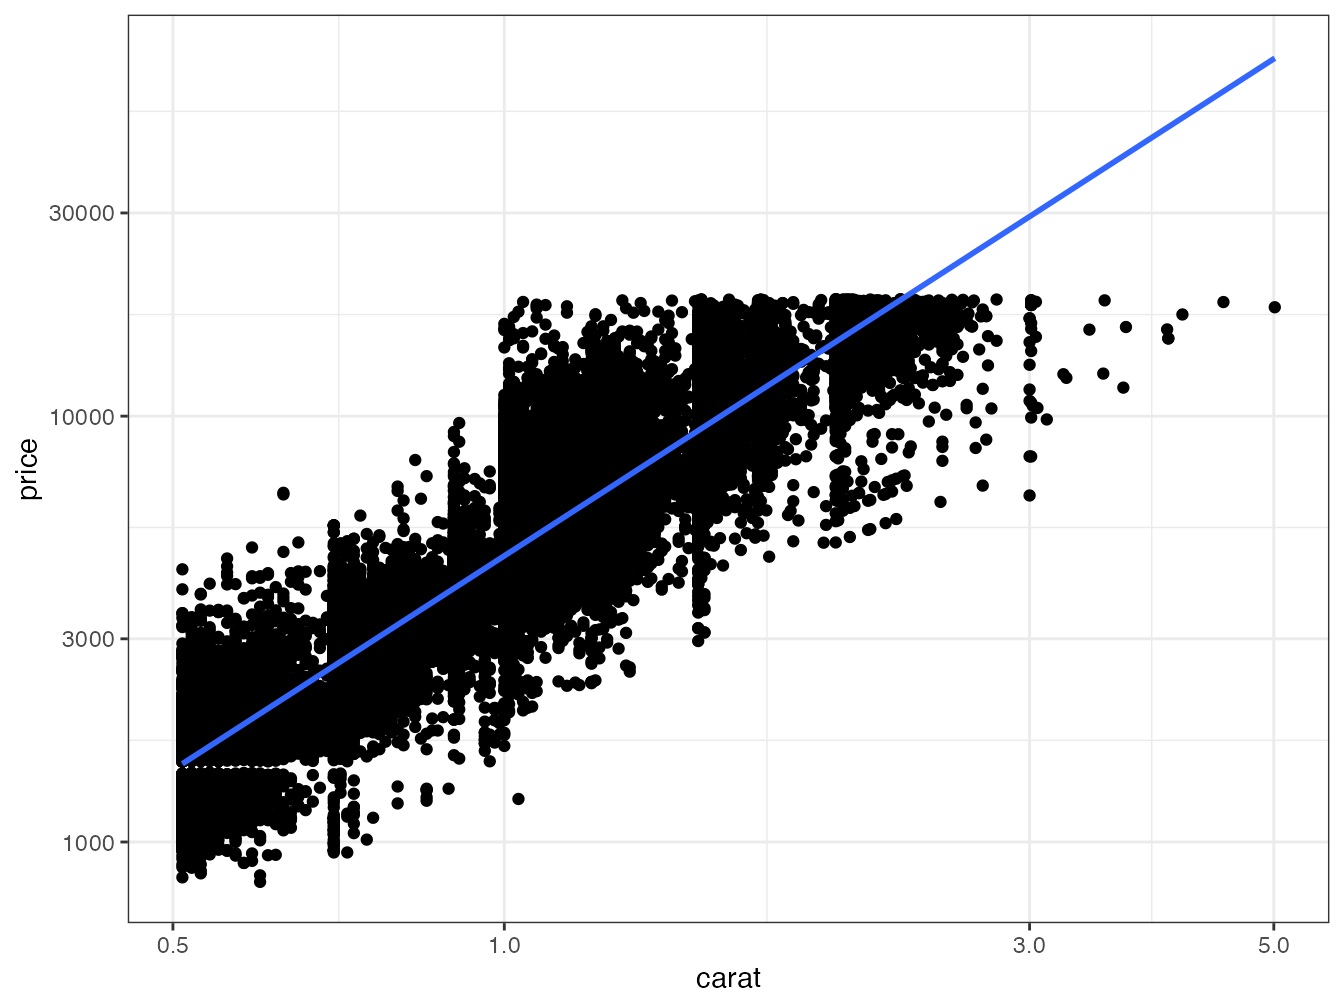
\includegraphics[width=0.8\linewidth]{WwR_files/figure-latex/diamonds-1} 

}

\caption{Price of diamonds according to their weight. Demonstration of the \textbf{ggplot2} code combined with tidyverse data processing.}\label{fig:diamonds}
\end{figure}

\normalsize

In this figure, two geometries (scatterplot and linear regression) share the same aesthetics (price vs.~weight in carats) which is therefore declared upstream, in the \texttt{ggplot()} function.

The tidyverse is documented in detail in \textcite{Wickham2016} and \textbf{ggplot2} in \textcite{Wickham2017}.

\section{Environments}\label{sec:environnements}

R's objects, data and functions, are named.
Since R is modular, with the ability to add any number of packages to it, it is very likely that name conflicts will arise.
To deal with them, R has a rigorous system of name precedence: code runs in a defined environment, inheriting from parent environments.

\subsection{Organization}\label{organization}

R starts in an empty environment.
Each loaded package creates a child environment to form a stack of environments, of which each new element is called a \enquote{child} of the previous one, which is its \enquote{parent}.

The console is in the global environment, the child of the last loaded package.

\scriptsize

\begin{Shaded}
\begin{Highlighting}[]
\FunctionTok{search}\NormalTok{()}
\end{Highlighting}
\end{Shaded}

\begin{verbatim}
##  [1] ".GlobalEnv"        "package:R6"       
##  [3] "package:entropart" "package:lubridate"
##  [5] "package:forcats"   "package:stringr"  
##  [7] "package:dplyr"     "package:purrr"    
##  [9] "package:readr"     "package:tidyr"    
## [11] "package:tibble"    "package:ggplot2"  
## [13] "package:tidyverse" "package:stats"    
## [15] "package:graphics"  "package:grDevices"
## [17] "package:utils"     "package:datasets" 
## [19] "package:methods"   "Autoloads"        
## [21] "package:base"
\end{verbatim}

\normalsize

The code of a function called from the console runs in a child environment of the global environment:

\scriptsize

\begin{Shaded}
\begin{Highlighting}[]
\CommentTok{\# Current environment}
\FunctionTok{environment}\NormalTok{()}
\end{Highlighting}
\end{Shaded}

\begin{verbatim}
## <environment: R_GlobalEnv>
\end{verbatim}

\begin{Shaded}
\begin{Highlighting}[]
\CommentTok{\# The function f displays its environment}
\NormalTok{f }\OtherTok{\textless{}{-}} \ControlFlowTok{function}\NormalTok{() }\FunctionTok{environment}\NormalTok{()}
\CommentTok{\# Display the environment of the function}
\FunctionTok{f}\NormalTok{()}
\end{Highlighting}
\end{Shaded}

\begin{verbatim}
## <environment: 0x13dcf5900>
\end{verbatim}

\begin{Shaded}
\begin{Highlighting}[]
\CommentTok{\# Parent environment of the function\textquotesingle{}s environment}
\FunctionTok{parent.env}\NormalTok{(}\FunctionTok{f}\NormalTok{())}
\end{Highlighting}
\end{Shaded}

\begin{verbatim}
## <environment: R_GlobalEnv>
\end{verbatim}

\normalsize

\subsection{Search}\label{search}

The search for ab object starts in the local environment.
If it is not found, it is searched in the parent environment, then in the parent of the parent, until the environments are exhausted, which generates an error indicating that the object was not found.

Example:

\scriptsize

\begin{Shaded}
\begin{Highlighting}[]
\CommentTok{\# Variable q defined in the global environment}
\NormalTok{q }\OtherTok{\textless{}{-}} \StringTok{"GlobalEnv"}
\CommentTok{\# Function defining q in its environment}
\NormalTok{qLocalFunction }\OtherTok{\textless{}{-}} \ControlFlowTok{function}\NormalTok{() \{}
\NormalTok{  q }\OtherTok{\textless{}{-}} \StringTok{"Function"}
  \FunctionTok{return}\NormalTok{(q)}
\NormalTok{\}}
\CommentTok{\# The local variable is returned}
\FunctionTok{qLocalFunction}\NormalTok{()}
\end{Highlighting}
\end{Shaded}

\begin{verbatim}
## [1] "Function"
\end{verbatim}

\begin{Shaded}
\begin{Highlighting}[]
\CommentTok{\# Poorly written function using a variable it does not define}
\NormalTok{qGlobalEnv }\OtherTok{\textless{}{-}} \ControlFlowTok{function}\NormalTok{() \{}
   \FunctionTok{return}\NormalTok{(q)}
\NormalTok{\}}
\CommentTok{\# The global environment variable is returned}
\FunctionTok{qGlobalEnv}\NormalTok{()}
\end{Highlighting}
\end{Shaded}

\begin{verbatim}
## [1] "GlobalEnv"
\end{verbatim}

\begin{Shaded}
\begin{Highlighting}[]
\CommentTok{\# Delete this variable}
\FunctionTok{rm}\NormalTok{(q)}
\CommentTok{\# The function base::q is returned}
\FunctionTok{qGlobalEnv}\NormalTok{()}
\end{Highlighting}
\end{Shaded}

\begin{verbatim}
## function (save = "default", status = 0, runLast = TRUE) 
## .Internal(quit(save, status, runLast))
## <bytecode: 0x12c8a44e0>
## <environment: namespace:base>
\end{verbatim}

\normalsize

The variable \texttt{q} is defined in the global environment.
The function \texttt{qLocalFunction} defines its own variable \texttt{q}.
Calling the function returns the its local value because it is in the function's environment.

The \texttt{qGlobalEnv} function returns the \texttt{q} variable that it does not define locally.
So it looks for it in its parent environment and finds the variable defined in the global environment.
By removing the variable from the global environment with \texttt{rm(q)}, the \texttt{qGlobalEnv()} function scans the stack of environments until it finds an object named \texttt{q} in the \textbf{base} package, which is the function to exit R.
It could have found another object if a package containing a \texttt{q} object had been loaded.

To avoid this erratic behavior, a function should \emph{never} call an object not defined in its own environment.

\subsection{Package namespaces}\label{package-namespaces}

It is time to define precisely what packages make visible.
Packages contain objects (functions and data) which they \emph{export} or not.
They are usually called by the \texttt{library()} function, which does two things:

\begin{itemize}
\tightlist
\item
  It \emph{loads} the package into memory, allowing access to all its objects with the syntax \texttt{package::object} for exported objects and \texttt{package:::object} for non-exported ones.
\item
  It then \emph{attaches} the package, which places its environment on top of the stack.
\end{itemize}

It is possible to detach a package with the \texttt{unloadNamespace()} function to remove it from the environment stack.
Example:

\scriptsize

\begin{Shaded}
\begin{Highlighting}[]
\CommentTok{\# entropart loaded and attached}
\FunctionTok{library}\NormalTok{(}\StringTok{"entropart"}\NormalTok{)}
\CommentTok{\# is it attached?}
\FunctionTok{isNamespaceLoaded}\NormalTok{(}\StringTok{"entropart"}\NormalTok{)}
\end{Highlighting}
\end{Shaded}

\begin{verbatim}
## [1] TRUE
\end{verbatim}

\begin{Shaded}
\begin{Highlighting}[]
\CommentTok{\# stack of environments}
\FunctionTok{search}\NormalTok{()}
\end{Highlighting}
\end{Shaded}

\begin{verbatim}
##  [1] ".GlobalEnv"        "package:R6"       
##  [3] "package:entropart" "package:lubridate"
##  [5] "package:forcats"   "package:stringr"  
##  [7] "package:dplyr"     "package:purrr"    
##  [9] "package:readr"     "package:tidyr"    
## [11] "package:tibble"    "package:ggplot2"  
## [13] "package:tidyverse" "package:stats"    
## [15] "package:graphics"  "package:grDevices"
## [17] "package:utils"     "package:datasets" 
## [19] "package:methods"   "Autoloads"        
## [21] "package:base"
\end{verbatim}

\begin{Shaded}
\begin{Highlighting}[]
\CommentTok{\# Diversity(), a function exported by entropart is found}
\FunctionTok{Diversity}\NormalTok{(}\DecValTok{1}\NormalTok{, }\AttributeTok{CheckArguments =} \ConstantTok{FALSE}\NormalTok{)}
\end{Highlighting}
\end{Shaded}

\begin{verbatim}
## None 
##    1
\end{verbatim}

\begin{Shaded}
\begin{Highlighting}[]
\CommentTok{\# Detach and unload entropart}
\FunctionTok{unloadNamespace}\NormalTok{(}\StringTok{"entropart"}\NormalTok{)}
\CommentTok{\# Is it attached?}
\FunctionTok{isNamespaceLoaded}\NormalTok{(}\StringTok{"entropart"}\NormalTok{)}
\end{Highlighting}
\end{Shaded}

\begin{verbatim}
## [1] FALSE
\end{verbatim}

\begin{Shaded}
\begin{Highlighting}[]
\CommentTok{\# Stack of environments, without entropart}
\FunctionTok{search}\NormalTok{()}
\end{Highlighting}
\end{Shaded}

\begin{verbatim}
##  [1] ".GlobalEnv"        "package:R6"       
##  [3] "package:lubridate" "package:forcats"  
##  [5] "package:stringr"   "package:dplyr"    
##  [7] "package:purrr"     "package:readr"    
##  [9] "package:tidyr"     "package:tibble"   
## [11] "package:ggplot2"   "package:tidyverse"
## [13] "package:stats"     "package:graphics" 
## [15] "package:grDevices" "package:utils"    
## [17] "package:datasets"  "package:methods"  
## [19] "Autoloads"         "package:base"
\end{verbatim}

\begin{Shaded}
\begin{Highlighting}[]
\CommentTok{\# Diversity() cannot be found}
\FunctionTok{tryCatch}\NormalTok{(}\FunctionTok{Diversity}\NormalTok{(}\DecValTok{1}\NormalTok{), }\AttributeTok{error =} \ControlFlowTok{function}\NormalTok{(e) }\FunctionTok{print}\NormalTok{(e))}
\end{Highlighting}
\end{Shaded}

\begin{verbatim}
## <simpleError in Diversity(1): could not find function "Diversity">
\end{verbatim}

\begin{Shaded}
\begin{Highlighting}[]
\CommentTok{\# but can be called with its full name}
\NormalTok{entropart}\SpecialCharTok{::}\FunctionTok{Diversity}\NormalTok{(}\DecValTok{1}\NormalTok{, }\AttributeTok{CheckArguments =} \ConstantTok{FALSE}\NormalTok{)}
\end{Highlighting}
\end{Shaded}

\begin{verbatim}
## None 
##    1
\end{verbatim}

\normalsize

Calling \texttt{entropart::Diversity()} loads the package (i.e., implicitly executes \texttt{loadNamespace("entropart")}) but does not attach it.

In practice, one should limit the number of attached packages to limit the risk of calling an unwanted function, homonymous to the desired function.
In critical cases, the full name of the function should be used: \texttt{package::function()}.

A common issue occurs with the \texttt{filter()} function of \textbf{dplyr}, which is the namesake of the \textbf{stats} function.
The \textbf{stats} package is usually loaded before \textbf{dplyr}, a package in the tidyverse.
Thus, \texttt{stats::filter()} must be called explicitly.

However, the \textbf{dplyr} or \textbf{tidyverse} package (which attaches all the tidyverse packages) can be loaded systematically by creating a \texttt{.RProfile} at the root of the project containing the command:

\scriptsize

\begin{Shaded}
\begin{Highlighting}[]
\FunctionTok{library}\NormalTok{(}\StringTok{"tidyverse"}\NormalTok{)}
\end{Highlighting}
\end{Shaded}

\normalsize

In this case, \textbf{dplyr} is loaded \emph{before} \textbf{stats} so its function is inaccessible.

\section{Measuring execution time}\label{measuring-execution-time}

The execution time of long code can be measured very simply by the \texttt{system.time} command.
For very short execution times, it is necessary to repeat the measurement: this is the purpose of the \textbf{microbenchmark} package.

\subsection{system.time}\label{system.time}

The function returns the execution time of the code.

\scriptsize

\begin{Shaded}
\begin{Highlighting}[]
\CommentTok{\# Mean absolute deviation of 1000 values in a uniform distribution, repeated 100 times}
\FunctionTok{system.time}\NormalTok{(}\ControlFlowTok{for}\NormalTok{ (i }\ControlFlowTok{in} \DecValTok{1}\SpecialCharTok{:}\DecValTok{100}\NormalTok{) }\FunctionTok{mad}\NormalTok{(}\FunctionTok{runif}\NormalTok{(}\DecValTok{1000}\NormalTok{)))}
\end{Highlighting}
\end{Shaded}

\begin{verbatim}
##    user  system elapsed 
##   0.009   0.000   0.010
\end{verbatim}

\normalsize

\subsection{microbenchmark}\label{microbenchmark}

The \textbf{microbenchmark} package is the most advanced.

The goal is to compare the speed of computing the square of a vector (or a number) by multiplying it by itself (\(x \times x\)) or by raising it to the power of 2 (\(x^2\)).

\scriptsize

\begin{Shaded}
\begin{Highlighting}[]
\CommentTok{\# Functions to test}
\NormalTok{f1 }\OtherTok{\textless{}{-}} \ControlFlowTok{function}\NormalTok{(x) x }\SpecialCharTok{*}\NormalTok{ x}
\NormalTok{f2 }\OtherTok{\textless{}{-}} \ControlFlowTok{function}\NormalTok{(x) x}\SpecialCharTok{\^{}}\DecValTok{2}
\NormalTok{f3 }\OtherTok{\textless{}{-}} \ControlFlowTok{function}\NormalTok{(x) x}\SpecialCharTok{\^{}}\FloatTok{2.1}
\NormalTok{f4 }\OtherTok{\textless{}{-}} \ControlFlowTok{function}\NormalTok{(x) x}\SpecialCharTok{\^{}}\DecValTok{3}
\CommentTok{\# Initialization}
\NormalTok{X }\OtherTok{\textless{}{-}} \FunctionTok{rnorm}\NormalTok{(}\DecValTok{10000}\NormalTok{)}
\CommentTok{\# Test}
\FunctionTok{library}\NormalTok{(}\StringTok{"microbenchmark"}\NormalTok{)}
\NormalTok{(mb }\OtherTok{\textless{}{-}} \FunctionTok{microbenchmark}\NormalTok{(}\FunctionTok{f1}\NormalTok{(X), }\FunctionTok{f2}\NormalTok{(X), }\FunctionTok{f3}\NormalTok{(X), }\FunctionTok{f4}\NormalTok{(X)))}
\end{Highlighting}
\end{Shaded}

\begin{verbatim}
## Unit: microseconds
##   expr     min       lq      mean   median       uq
##  f1(X)   1.927   7.9540  20.60414  10.9060  19.6595
##  f2(X)   4.510   9.8810  22.08260  13.1610  21.9555
##  f3(X) 101.557 111.7660 191.55282 126.9565 157.3990
##  f4(X) 137.104 146.8005 231.05550 154.3445 236.5495
##       max neval
##   524.882   100
##   517.092   100
##  1262.390   100
##  1377.231   100
\end{verbatim}

\normalsize

The returned table contains the minimum, median, mean, max and first and third quartile times, as well as the number of repetitions.
The median value is to be compared.
The number of repetitions is by default 100, to be modulated (argument \texttt{times}) according to the complexity of the calculation.

The test result, a \texttt{microbenchmark} object, is a raw table of execution times.
The statistical analysis is done by the \texttt{print} and \texttt{summary} methods.
To choose the columns to display, use the following syntax:

\scriptsize

\begin{Shaded}
\begin{Highlighting}[]
\FunctionTok{summary}\NormalTok{(mb)[, }\FunctionTok{c}\NormalTok{(}\StringTok{"expr"}\NormalTok{, }\StringTok{"median"}\NormalTok{)]}
\end{Highlighting}
\end{Shaded}

\begin{verbatim}
##    expr   median
## 1 f1(X)  10.9060
## 2 f2(X)  13.1610
## 3 f3(X) 126.9565
## 4 f4(X) 154.3445
\end{verbatim}

\normalsize

To make calculations on these results, we must store them in a variable.
To prevent the results from being displayed in the console, the simplest solution is to use the \texttt{capture.output} function by assigning its result to a variable.

\scriptsize

\begin{Shaded}
\begin{Highlighting}[]
\NormalTok{dummy }\OtherTok{\textless{}{-}} \FunctionTok{capture.output}\NormalTok{(mbs }\OtherTok{\textless{}{-}} \FunctionTok{summary}\NormalTok{(mb))}
\end{Highlighting}
\end{Shaded}

\normalsize

The previous test is displayed again.

\scriptsize

\begin{Shaded}
\begin{Highlighting}[]
\FunctionTok{summary}\NormalTok{(mb)[, }\FunctionTok{c}\NormalTok{(}\StringTok{"expr"}\NormalTok{, }\StringTok{"median"}\NormalTok{)]}
\end{Highlighting}
\end{Shaded}

\begin{verbatim}
##    expr   median
## 1 f1(X)  10.9060
## 2 f2(X)  13.1610
## 3 f3(X) 126.9565
## 4 f4(X) 154.3445
\end{verbatim}

\normalsize

The computation time is about the same between \(x \times x\) and \(x^2\).
The power calculation is much longer, especially if the power is not integer, because it requires a logarithm calculation.
The computation of the power 2 is therefore optimized by R to avoid the use of log.

Two graphical representations are available: the violins represent the probability density of the execution time; the boxplots are classical.

\scriptsize

\begin{Shaded}
\begin{Highlighting}[]
\FunctionTok{library}\NormalTok{(}\StringTok{"ggplot2"}\NormalTok{)}
\FunctionTok{autoplot}\NormalTok{(mb)}
\end{Highlighting}
\end{Shaded}

\begin{center}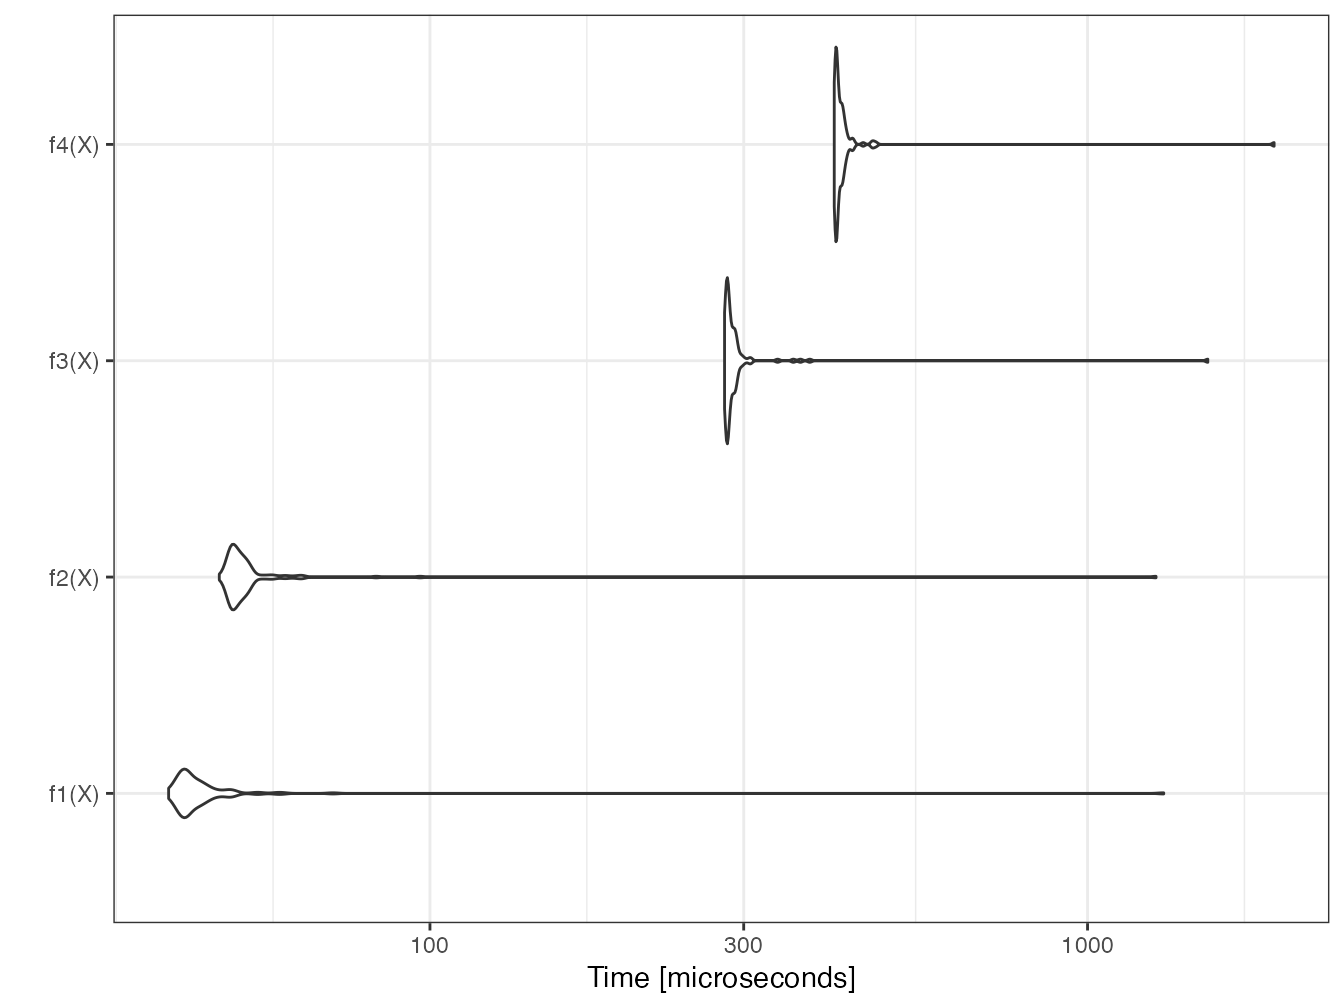
\includegraphics[width=0.8\linewidth]{WwR_files/figure-latex/boxplot-1} \end{center}

\begin{Shaded}
\begin{Highlighting}[]
\FunctionTok{boxplot}\NormalTok{(mb)}
\end{Highlighting}
\end{Shaded}

\begin{center}
\includegraphics[width=0.8\linewidth]{WwR_files/figure-latex/boxplot-2} \end{center}

\normalsize

\subsection{Profiling}\label{profiling}

\textbf{profvis} is RStudio's profiling tool.

It tracks the execution time of each line of code and the memory used.
The goal is to detect slow code portions that need to be improved.

\scriptsize

\begin{Shaded}
\begin{Highlighting}[]
\FunctionTok{library}\NormalTok{(profvis)}
\NormalTok{p }\OtherTok{\textless{}{-}} \FunctionTok{profvis}\NormalTok{(\{}
  \CommentTok{\# Cosine calculations}
  \FunctionTok{cos}\NormalTok{(}\FunctionTok{runif}\NormalTok{(}\DecValTok{10}\SpecialCharTok{\^{}}\DecValTok{7}\NormalTok{))}
  \CommentTok{\# 1/2 second pause}
  \FunctionTok{pause}\NormalTok{(}\DecValTok{1} \SpecialCharTok{/} \DecValTok{2}\NormalTok{)}
\NormalTok{\})}
\NormalTok{htmlwidgets}\SpecialCharTok{::}\FunctionTok{saveWidget}\NormalTok{(p, }\StringTok{"docs/profile.html"}\NormalTok{)}
\end{Highlighting}
\end{Shaded}

\normalsize

The result is an HTML file containing the profiling report\footnote{\url{https://EricMarcon.github.io/WorkingWithR/profile.html}}.
It can be observed that the time to draw the random numbers is similar to that of the cosine calculation.

Read the complete documentation\footnote{\url{https://rstudio.github.io/profvis/}} on the RStudio website.

\section{Loops}\label{loops}

The most frequent case of long code to execute is loops: the same code is repeated a large number of times.

\subsection{Vector functions}\label{vector-functions}

Most of R's functions are vector functions: loops are processed internally, extremely fast.
Therefore, you should think in terms of vectors rather than scalars.

\scriptsize

\begin{Shaded}
\begin{Highlighting}[]
\CommentTok{\# Draw two vectors of three random numbers between 0 and 1}
\NormalTok{x1 }\OtherTok{\textless{}{-}} \FunctionTok{runif}\NormalTok{(}\DecValTok{3}\NormalTok{)}
\NormalTok{x2 }\OtherTok{\textless{}{-}} \FunctionTok{runif}\NormalTok{(}\DecValTok{3}\NormalTok{)}
\CommentTok{\# Square root of the three numbers in x1}
\FunctionTok{sqrt}\NormalTok{(x1)}
\end{Highlighting}
\end{Shaded}

\begin{verbatim}
## [1] 0.9427738 0.8665204 0.4586981
\end{verbatim}

\begin{Shaded}
\begin{Highlighting}[]
\CommentTok{\# Respective sums of the three numbers of x1 and x2}
\NormalTok{x1 }\SpecialCharTok{+}\NormalTok{ x2}
\end{Highlighting}
\end{Shaded}

\begin{verbatim}
## [1] 1.6262539 1.6881583 0.9063973
\end{verbatim}

\normalsize

We also have to write vector functions on their first argument.
The function \texttt{lnq} of the package \textbf{entropart} returns the deformed logarithm of order \(q\) of a number \(x\).

\scriptsize

\begin{Shaded}
\begin{Highlighting}[]
\CommentTok{\# Code of the function}
\NormalTok{entropart}\SpecialCharTok{::}\NormalTok{lnq}
\end{Highlighting}
\end{Shaded}

\begin{verbatim}
## function (x, q) 
## {
##     if (q == 1) {
##         return(log(x))
##     }
##     else {
##         Log <- (x^(1 - q) - 1)/(1 - q)
##         Log[x < 0] <- NA
##         return(Log)
##     }
## }
## <bytecode: 0x13ed2a4a8>
## <environment: namespace:entropart>
\end{verbatim}

\normalsize

For a function to be vector, each line of its code must allow the first argument to be treated as a vector.
Here: \texttt{log(x)} and \texttt{x\^{}} are a vector function and operator and the condition \texttt{{[}x\ \textless{}\ 0{]}} also returns a vector.

\subsection{lapply}\label{lapply}

Code that cannot be written as a vector function requires loops.

\texttt{lapply()} applies a function to each element of a list.
There are several versions of this function:

\begin{itemize}
\tightlist
\item
  \texttt{lapply()} returns a list (and saves the time of rearranging them in an array).
\item
  \texttt{sapply()} returns a dataframe by collapsing the lists (this is done by the \texttt{simplify2array()} function).
\item
  \texttt{vapply()} is almost identical but requires that the data type of the result be provided.
\end{itemize}

\scriptsize

\begin{Shaded}
\begin{Highlighting}[]
\CommentTok{\# Draw 1000 values in a uniform distribution}
\NormalTok{x1 }\OtherTok{\textless{}{-}} \FunctionTok{runif}\NormalTok{(}\DecValTok{1000}\NormalTok{)}
\CommentTok{\# The square root can be calculated for the vector or each value }
\FunctionTok{identical}\NormalTok{(}\FunctionTok{sqrt}\NormalTok{(x1), }\FunctionTok{sapply}\NormalTok{(x1, }\AttributeTok{FUN =}\NormalTok{ sqrt))}
\end{Highlighting}
\end{Shaded}

\begin{verbatim}
## [1] TRUE
\end{verbatim}

\begin{Shaded}
\begin{Highlighting}[]
\NormalTok{mb }\OtherTok{\textless{}{-}} \FunctionTok{microbenchmark}\NormalTok{(}
  \FunctionTok{sqrt}\NormalTok{(x1), }
  \FunctionTok{lapply}\NormalTok{(x1, }\AttributeTok{FUN =}\NormalTok{ sqrt), }
  \FunctionTok{sapply}\NormalTok{(x1, }\AttributeTok{FUN =}\NormalTok{ sqrt), }
  \FunctionTok{vapply}\NormalTok{(x1, }\AttributeTok{FUN =}\NormalTok{ sqrt, }\AttributeTok{FUN.VALUE =} \DecValTok{0}\NormalTok{)}
\NormalTok{)}
\FunctionTok{summary}\NormalTok{(mb)[, }\FunctionTok{c}\NormalTok{(}\StringTok{"expr"}\NormalTok{, }\StringTok{"median"}\NormalTok{)]}
\end{Highlighting}
\end{Shaded}

\begin{verbatim}
##                                    expr   median
## 1                              sqrt(x1)   1.5990
## 2                lapply(x1, FUN = sqrt) 143.1515
## 3                sapply(x1, FUN = sqrt) 175.2545
## 4 vapply(x1, FUN = sqrt, FUN.VALUE = 0) 139.1950
\end{verbatim}

\normalsize

\texttt{lapply()} is much slower than a vector function.
\texttt{sapply()} requires more time for \texttt{simplify2array()}, which must detect how to gather the results.
Finally, \texttt{vapply()} saves the time of determining the data type of the result and allows for faster computation with little effort.

\subsection{For loops}\label{for-loops}

Loops are handled by the \texttt{for} function.
They have the reputation of being slow in R because the code inside the loop must be interpreted at each execution.
This is no longer the case since version 3.5 of R: loops are compiled systematically before execution.
The behavior of the just-in-time compiler is defined by the \texttt{enableJIT} function.
The default level is 3: all functions are compiled, and loops in the code are compiled too.

To evaluate the performance gain, the following code removes all automatic compilation, and compares the same loop compiled or not.

\scriptsize

\begin{Shaded}
\begin{Highlighting}[]
\FunctionTok{library}\NormalTok{(}\StringTok{"compiler"}\NormalTok{)}
\CommentTok{\# No automatic compilation}
\FunctionTok{enableJIT}\NormalTok{(}\AttributeTok{level =} \DecValTok{0}\NormalTok{)}
\end{Highlighting}
\end{Shaded}

\begin{verbatim}
## [1] 3
\end{verbatim}

\begin{Shaded}
\begin{Highlighting}[]
\CommentTok{\# Loop to calculate the square root of a vector}
\NormalTok{loop }\OtherTok{\textless{}{-}} \ControlFlowTok{function}\NormalTok{(x) \{}
  \CommentTok{\# Initialization of the result vector, essential}
\NormalTok{  root }\OtherTok{\textless{}{-}} \FunctionTok{vector}\NormalTok{(}\StringTok{"numeric"}\NormalTok{, }\AttributeTok{length =} \FunctionTok{length}\NormalTok{(x))}
  \CommentTok{\# Loop}
  \ControlFlowTok{for}\NormalTok{ (i }\ControlFlowTok{in} \DecValTok{1}\SpecialCharTok{:}\FunctionTok{length}\NormalTok{(x)) root[i] }\OtherTok{\textless{}{-}} \FunctionTok{sqrt}\NormalTok{(x[i])}
  \FunctionTok{return}\NormalTok{(root)}
\NormalTok{\}}
\CommentTok{\# Compiled version}
\NormalTok{loop2 }\OtherTok{\textless{}{-}} \FunctionTok{cmpfun}\NormalTok{(loop)}
\CommentTok{\# Comparison}
\NormalTok{mb }\OtherTok{\textless{}{-}} \FunctionTok{microbenchmark}\NormalTok{(}\FunctionTok{loop}\NormalTok{(x1), }\FunctionTok{loop2}\NormalTok{(x1))}
\NormalTok{(mbs }\OtherTok{\textless{}{-}} \FunctionTok{summary}\NormalTok{(mb)[, }\FunctionTok{c}\NormalTok{(}\StringTok{"expr"}\NormalTok{, }\StringTok{"median"}\NormalTok{)])}
\end{Highlighting}
\end{Shaded}

\begin{verbatim}
##        expr   median
## 1  loop(x1) 358.3605
## 2 loop2(x1)  43.3780
\end{verbatim}

\begin{Shaded}
\begin{Highlighting}[]
\CommentTok{\# Automatic compilation by default since version 3.5}
\FunctionTok{enableJIT}\NormalTok{(}\AttributeTok{level =} \DecValTok{3}\NormalTok{)}
\end{Highlighting}
\end{Shaded}

\begin{verbatim}
## [1] 0
\end{verbatim}

\normalsize

The gain is considerable: from 1 to \texttt{8}.

For loops are now much faster than \texttt{vapply}.

\scriptsize

\begin{Shaded}
\begin{Highlighting}[]
\CommentTok{\# Test}
\NormalTok{mb }\OtherTok{\textless{}{-}} \FunctionTok{microbenchmark}\NormalTok{(}\FunctionTok{vapply}\NormalTok{(x1, }\AttributeTok{FUN =}\NormalTok{ sqrt, }\DecValTok{0}\NormalTok{), }\FunctionTok{loop}\NormalTok{(x1))}
\FunctionTok{summary}\NormalTok{(mb)[, }\FunctionTok{c}\NormalTok{(}\StringTok{"expr"}\NormalTok{, }\StringTok{"median"}\NormalTok{)]}
\end{Highlighting}
\end{Shaded}

\begin{verbatim}
##                        expr   median
## 1 vapply(x1, FUN = sqrt, 0) 133.5575
## 2                  loop(x1)  42.0660
\end{verbatim}

\normalsize

Be careful, the performance test can be misleading:

\scriptsize

\begin{Shaded}
\begin{Highlighting}[]
\CommentTok{\# Preparing the result vector}
\NormalTok{root }\OtherTok{\textless{}{-}} \FunctionTok{vector}\NormalTok{(}\StringTok{"numeric"}\NormalTok{, }\AttributeTok{length =} \FunctionTok{length}\NormalTok{(x1))}
\CommentTok{\# Test}
\NormalTok{mb }\OtherTok{\textless{}{-}} \FunctionTok{microbenchmark}\NormalTok{(}
  \FunctionTok{vapply}\NormalTok{(x1, }\AttributeTok{FUN =}\NormalTok{ sqrt, }\DecValTok{0}\NormalTok{), }
  \ControlFlowTok{for}\NormalTok{ (i }\ControlFlowTok{in} \DecValTok{1}\SpecialCharTok{:}\FunctionTok{length}\NormalTok{(x1)) root[i] }\OtherTok{\textless{}{-}} \FunctionTok{sqrt}\NormalTok{(x1[i])}
\NormalTok{)}
\FunctionTok{summary}\NormalTok{(mb)[, }\FunctionTok{c}\NormalTok{(}\StringTok{"expr"}\NormalTok{, }\StringTok{"median"}\NormalTok{)]}
\end{Highlighting}
\end{Shaded}

\begin{verbatim}
##                                             expr   median
## 1                      vapply(x1, FUN = sqrt, 0)  148.666
## 2 for (i in 1:length(x1)) root[i] <- sqrt(x1[i]) 1449.145
\end{verbatim}

\normalsize

In this code, the for loop is not compiled so it is much slower than in its normal use (in a function or at the top level of the code).

The long loops allow tracking of their progress by a text bar, which is another advantage.
The following function executes pauses of one tenth of a second for the time passed in parameter (in seconds).

\scriptsize

\begin{Shaded}
\begin{Highlighting}[]
\NormalTok{loop\_monitored }\OtherTok{\textless{}{-}} \ControlFlowTok{function}\NormalTok{(}\AttributeTok{duration =} \DecValTok{1}\NormalTok{) \{}
  \CommentTok{\# Progress bar}
\NormalTok{  pgb }\OtherTok{\textless{}{-}} \FunctionTok{txtProgressBar}\NormalTok{(}\AttributeTok{min =} \DecValTok{0}\NormalTok{, }\AttributeTok{max =}\NormalTok{ duration }\SpecialCharTok{*} \DecValTok{10}\NormalTok{)}
  \CommentTok{\# Loop}
  \ControlFlowTok{for}\NormalTok{ (i }\ControlFlowTok{in} \DecValTok{1}\SpecialCharTok{:}\NormalTok{(duration }\SpecialCharTok{*} \DecValTok{10}\NormalTok{)) \{}
    \CommentTok{\# Pause for a tenth of a second}
    \FunctionTok{Sys.sleep}\NormalTok{(}\DecValTok{1} \SpecialCharTok{/} \DecValTok{10}\NormalTok{)}
    \CommentTok{\# Track progress}
    \FunctionTok{setTxtProgressBar}\NormalTok{(pgb, i)}
\NormalTok{  \}}
\NormalTok{\}}
\FunctionTok{loop\_monitored}\NormalTok{()}
\end{Highlighting}
\end{Shaded}

\begin{verbatim}
## ============================================================
\end{verbatim}

\normalsize

\subsection{replicate}\label{replicate}

\texttt{replicate()} repeats a statement.

\scriptsize

\begin{Shaded}
\begin{Highlighting}[]
\FunctionTok{replicate}\NormalTok{(}\DecValTok{3}\NormalTok{, }\FunctionTok{runif}\NormalTok{(}\DecValTok{1}\NormalTok{))}
\end{Highlighting}
\end{Shaded}

\begin{verbatim}
## [1] 0.9453453 0.5262818 0.7233425
\end{verbatim}

\normalsize

This code is equivalent to \texttt{runif(3)}, with performance similar to \texttt{vapply}: 50 to 100 times slower than a vector function.

\scriptsize

\begin{Shaded}
\begin{Highlighting}[]
\NormalTok{mb }\OtherTok{\textless{}{-}} \FunctionTok{microbenchmark}\NormalTok{(}\FunctionTok{replicate}\NormalTok{(}\FloatTok{1E3}\NormalTok{, }\FunctionTok{runif}\NormalTok{(}\DecValTok{1}\NormalTok{)), }\FunctionTok{runif}\NormalTok{(}\FloatTok{1E3}\NormalTok{))}
\FunctionTok{summary}\NormalTok{(mb)[, }\FunctionTok{c}\NormalTok{(}\StringTok{"expr"}\NormalTok{, }\StringTok{"median"}\NormalTok{)]}
\end{Highlighting}
\end{Shaded}

\begin{verbatim}
##                        expr  median
## 1 replicate(1000, runif(1)) 833.325
## 2               runif(1000)   6.642
\end{verbatim}

\normalsize

\subsection{Vectorize}\label{vectorize}

\texttt{Vectorize()} makes a function that is not vectorized, by loops.
Write the loops instead.

\subsection{Marginal statistics}\label{marginal-statistics}

\texttt{apply} applies a function to the rows or columns of a two dimensional object.

\texttt{colSums} and similar functions (\texttt{rowSums}, \texttt{colMeans}, \texttt{rowMeans}) are optimized.

\scriptsize

\begin{Shaded}
\begin{Highlighting}[]
\CommentTok{\# Sum of the numeric columns of the diamonds dataset of ggplot2}
\CommentTok{\# Loop identical to the action of apply(, 2, )}
\NormalTok{loop\_sum }\OtherTok{\textless{}{-}} \ControlFlowTok{function}\NormalTok{(table) \{}
\NormalTok{  the\_sum }\OtherTok{\textless{}{-}} \FunctionTok{vector}\NormalTok{(}\StringTok{"numeric"}\NormalTok{, }\AttributeTok{length =} \FunctionTok{ncol}\NormalTok{(table))}
  \ControlFlowTok{for}\NormalTok{ (i }\ControlFlowTok{in} \DecValTok{1}\SpecialCharTok{:}\FunctionTok{ncol}\NormalTok{(table)) the\_sum[i] }\OtherTok{\textless{}{-}} \FunctionTok{sum}\NormalTok{(table[, i])}
  \FunctionTok{return}\NormalTok{(the\_sum)}
\NormalTok{\}}
\NormalTok{mb }\OtherTok{\textless{}{-}} \FunctionTok{microbenchmark}\NormalTok{(}
  \FunctionTok{loop\_sum}\NormalTok{(diamonds[}\SpecialCharTok{{-}}\NormalTok{(}\DecValTok{2}\SpecialCharTok{:}\DecValTok{4}\NormalTok{)]),}
  \FunctionTok{apply}\NormalTok{(diamonds[}\SpecialCharTok{{-}}\NormalTok{(}\DecValTok{2}\SpecialCharTok{:}\DecValTok{4}\NormalTok{)], }\DecValTok{2}\NormalTok{, sum), }
  \FunctionTok{colSums}\NormalTok{(diamonds[}\SpecialCharTok{{-}}\NormalTok{(}\DecValTok{2}\SpecialCharTok{:}\DecValTok{4}\NormalTok{)])}
\NormalTok{)}
\FunctionTok{summary}\NormalTok{(mb)[, }\FunctionTok{c}\NormalTok{(}\StringTok{"expr"}\NormalTok{, }\StringTok{"median"}\NormalTok{)]}
\end{Highlighting}
\end{Shaded}

\begin{verbatim}
##                              expr   median
## 1      loop_sum(diamonds[-(2:4)]) 1.890694
## 2 apply(diamonds[-(2:4)], 2, sum) 4.833736
## 3       colSums(diamonds[-(2:4)]) 1.386661
\end{verbatim}

\normalsize

\texttt{apply} clarifies the code but is slower than the loop, which is only slightly slower than \texttt{colSums}.

\section{C++ code}\label{sec:cpp}

Integrating C++ code into R is greatly simplified by the \textbf{Rcpp} package but is still difficult to debug and therefore should be reserved for very simple code (to avoid errors) repeated a large number of times (to be worth the effort).
The preparation and verification of the data must be done in R, as well as the processing and presentation of the results.

The common practice is to include C++ code in a package, but running it outside a package is possible:

\begin{itemize}
\tightlist
\item
  C++ code can be included in a C++ document (file with extension \texttt{.cpp}): it is compiled by the \texttt{sourceCpp()} command, which creates the R functions to call the C++ code.
\item
  In an RMarkdown document, Rcpp code snippets can be created to insert the C++ code: they are compiled and interfaced to R at the time of knitting.
\end{itemize}

The following example shows how to create a C++ function to calculate the double of a numerical vector.

\scriptsize

\begin{Shaded}
\begin{Highlighting}[]
\PreprocessorTok{\#include }\ImportTok{\textless{}Rcpp.h\textgreater{}}
\KeywordTok{using} \KeywordTok{namespace}\NormalTok{ Rcpp}\OperatorTok{;}

\CommentTok{// [[Rcpp::export]]}
\NormalTok{NumericVector timesTwo}\OperatorTok{(}\NormalTok{NumericVector x}\OperatorTok{)} \OperatorTok{\{}
  \ControlFlowTok{return}\NormalTok{ x }\OperatorTok{*} \DecValTok{2}\OperatorTok{;}
\OperatorTok{\}}
\end{Highlighting}
\end{Shaded}

\normalsize

An R function with the same name as the C++ function is now available.

\scriptsize

\begin{Shaded}
\begin{Highlighting}[]
\FunctionTok{timesTwo}\NormalTok{(}\DecValTok{1}\SpecialCharTok{:}\DecValTok{5}\NormalTok{)}
\end{Highlighting}
\end{Shaded}

\begin{verbatim}
## [1]  2  4  6  8 10
\end{verbatim}

\normalsize

The performance is two orders of magnitude faster than the R code (see the case study, section \ref{sec:cas}).

\section{Parallelizing R}\label{parallelizing-r}

When long computations can be split into independent tasks, the simultaneous (\emph{parallel}) execution of these tasks reduces the total computation time to that of the longest task, to which is added the cost of setting up the parallelization (creation of the tasks, recovery of the results\ldots).

Read Josh Errickson's excellent introduction\footnote{\url{http://dept.stat.lsa.umich.edu/~jerrick/courses/stat701/notes/parallel.html}} which details the issues and constraints of parallelization.

Two mechanisms are available for parallel code execution:

\begin{itemize}
\tightlist
\item
  \emph{fork}: the running process is duplicated on multiple cores of the computing computer's processor.
  This is the simplest method but it does not work on Windows (it is a limitation of the operating system).
\item
  \emph{Socket}: a cluster is constituted, either physically (a set of computers running R is necessary) or logically (an instance of R on each core of the computer used).
  The members of the cluster communicate through the network (the internal network of the computer is used in a logical cluster).
\end{itemize}

Different R packages allow to implement these mechanisms.

\subsection{mclapply (fork)}\label{mclapply-fork}

The \texttt{mclapply} function of the \textbf{parallel} package has the same syntax as \texttt{lapply} but parallelizes the execution of loops.
On Windows, it has no effect since the system does not allow \emph{fork}: it simply calls \texttt{lapply}.
However, a workaround exists to emulate \texttt{mclapply} on Windows by calling \texttt{parLapply}, which uses a cluster.

\scriptsize

\begin{Shaded}
\begin{Highlighting}[]
\DocumentationTok{\#\# mclapply.hack.R}
\DocumentationTok{\#\#}
\DocumentationTok{\#\# Nathan VanHoudnos}
\DocumentationTok{\#\# nathanvan AT northwestern FULL STOP edu}
\DocumentationTok{\#\# July 14, 2014}
\DocumentationTok{\#\#}
\DocumentationTok{\#\# A script to implement a hackish version of }
\DocumentationTok{\#\# parallel:mclapply() on Windows machines.}
\DocumentationTok{\#\# On Linux or Mac, the script has no effect}
\DocumentationTok{\#\# beyond loading the parallel library. }

\FunctionTok{require}\NormalTok{(parallel)    }

\DocumentationTok{\#\# Define the hack}
\CommentTok{\# mc.cores argument added: Eric Marcon}
\NormalTok{mclapply.hack }\OtherTok{\textless{}{-}} \ControlFlowTok{function}\NormalTok{(..., }\AttributeTok{mc.cores =} \FunctionTok{detectCores}\NormalTok{()) \{}
  \DocumentationTok{\#\# Create a cluster}
\NormalTok{  size.of.list }\OtherTok{\textless{}{-}} \FunctionTok{length}\NormalTok{(}\FunctionTok{list}\NormalTok{(...)[[}\DecValTok{1}\NormalTok{]])}
\NormalTok{  cl }\OtherTok{\textless{}{-}} \FunctionTok{makeCluster}\NormalTok{(}\FunctionTok{min}\NormalTok{(size.of.list, mc.cores))}
  
  \DocumentationTok{\#\# Find out the names of the loaded packages }
\NormalTok{  loaded.package.names }\OtherTok{\textless{}{-}} \FunctionTok{c}\NormalTok{(}
    \DocumentationTok{\#\# Base packages}
    \FunctionTok{sessionInfo}\NormalTok{()}\SpecialCharTok{$}\NormalTok{basePkgs,}
    \DocumentationTok{\#\# Additional packages}
    \FunctionTok{names}\NormalTok{(}\FunctionTok{sessionInfo}\NormalTok{()}\SpecialCharTok{$}\NormalTok{otherPkgs)}
\NormalTok{  )}
  
  \FunctionTok{tryCatch}\NormalTok{(}
\NormalTok{    \{}
      \DocumentationTok{\#\# Copy over all of the objects within scope to}
      \DocumentationTok{\#\# all clusters. }
\NormalTok{      this.env }\OtherTok{\textless{}{-}} \FunctionTok{environment}\NormalTok{()}
      \ControlFlowTok{while}\NormalTok{ (}\FunctionTok{identical}\NormalTok{(this.env, }\FunctionTok{globalenv}\NormalTok{()) }\SpecialCharTok{==} \ConstantTok{FALSE}\NormalTok{) \{}
        \FunctionTok{clusterExport}\NormalTok{(}
\NormalTok{          cl,}
          \FunctionTok{ls}\NormalTok{(}\AttributeTok{all.names =} \ConstantTok{TRUE}\NormalTok{, }\AttributeTok{env =}\NormalTok{ this.env),}
          \AttributeTok{envir =}\NormalTok{ this.env}
\NormalTok{        )}
\NormalTok{        this.env }\OtherTok{\textless{}{-}} \FunctionTok{parent.env}\NormalTok{(}\FunctionTok{environment}\NormalTok{())}
\NormalTok{      \}}
      \FunctionTok{clusterExport}\NormalTok{(}
\NormalTok{        cl,}
        \FunctionTok{ls}\NormalTok{(}\AttributeTok{all.names =} \ConstantTok{TRUE}\NormalTok{, }\AttributeTok{env =} \FunctionTok{globalenv}\NormalTok{()),}
        \AttributeTok{envir =} \FunctionTok{globalenv}\NormalTok{()}
\NormalTok{      )}
      
      \DocumentationTok{\#\# Load the libraries on all the clusters}
      \DocumentationTok{\#\# N.B. length(cl) returns the number of clusters}
      \FunctionTok{parLapply}\NormalTok{(}
        \AttributeTok{cl =}\NormalTok{ cl, }
        \AttributeTok{X =} \DecValTok{1}\SpecialCharTok{:}\FunctionTok{length}\NormalTok{(cl), }
        \AttributeTok{fun =} \ControlFlowTok{function}\NormalTok{(xx)\{}
          \FunctionTok{lapply}\NormalTok{(}
\NormalTok{            loaded.package.names, }
            \AttributeTok{FUN =} \ControlFlowTok{function}\NormalTok{(yy) \{}
              \FunctionTok{require}\NormalTok{(yy, }\AttributeTok{character.only =} \ConstantTok{TRUE}\NormalTok{)}
\NormalTok{            \}}
\NormalTok{          )}
\NormalTok{        \}}
\NormalTok{      )}
      
      \DocumentationTok{\#\# Run the lapply in parallel }
      \FunctionTok{return}\NormalTok{(}\FunctionTok{parLapply}\NormalTok{(cl, ...))}
\NormalTok{    \}, }
    \AttributeTok{finally =}\NormalTok{ \{        }
      \DocumentationTok{\#\# Stop the cluster}
      \FunctionTok{stopCluster}\NormalTok{(cl)}
\NormalTok{    \}}
\NormalTok{  )}
\NormalTok{\}}

\DocumentationTok{\#\# Warn the user if they are using Windows}
\ControlFlowTok{if}\NormalTok{ (}\FunctionTok{Sys.info}\NormalTok{()[[}\StringTok{\textquotesingle{}sysname\textquotesingle{}}\NormalTok{]] }\SpecialCharTok{==} \StringTok{\textquotesingle{}Windows\textquotesingle{}}\NormalTok{) \{}
  \FunctionTok{message}\NormalTok{(}\FunctionTok{paste}\NormalTok{(}
    \StringTok{"}\SpecialCharTok{\textbackslash{}n}\StringTok{"}\NormalTok{, }
    \StringTok{"   *** Microsoft Windows detected ***}\SpecialCharTok{\textbackslash{}n}\StringTok{"}\NormalTok{,}
    \StringTok{"   }\SpecialCharTok{\textbackslash{}n}\StringTok{"}\NormalTok{,}
    \StringTok{"   For technical reasons, the MS Windows version of mclapply()}\SpecialCharTok{\textbackslash{}n}\StringTok{"}\NormalTok{,}
    \StringTok{"   is implemented as a serial function instead of a parallel}\SpecialCharTok{\textbackslash{}n}\StringTok{"}\NormalTok{,}
    \StringTok{"   function."}\NormalTok{,}
    \StringTok{"   }\SpecialCharTok{\textbackslash{}n\textbackslash{}n}\StringTok{"}\NormalTok{,}
    \StringTok{"   As a quick hack, we replace this serial version of mclapply()}\SpecialCharTok{\textbackslash{}n}\StringTok{"}\NormalTok{,}
    \StringTok{"   with a wrapper to parLapply() for this R session. Please see}\SpecialCharTok{\textbackslash{}n\textbackslash{}n}\StringTok{"}\NormalTok{,}
    \StringTok{"     http://www.stat.cmu.edu/\textasciitilde{}nmv/2014/07/14/}
\StringTok{    implementing{-}mclapply{-}on{-}windows }\SpecialCharTok{\textbackslash{}n\textbackslash{}n}\StringTok{"}\NormalTok{,}
    \StringTok{"   for details.}\SpecialCharTok{\textbackslash{}n\textbackslash{}n}\StringTok{"}\NormalTok{)}
\NormalTok{  )}
\NormalTok{\}}

\DocumentationTok{\#\# If the OS is Windows, set mclapply to the}
\DocumentationTok{\#\# the hackish version. Otherwise, leave the}
\DocumentationTok{\#\# definition alone. }
\NormalTok{mclapply }\OtherTok{\textless{}{-}} \ControlFlowTok{switch}\NormalTok{(}
  \FunctionTok{Sys.info}\NormalTok{()[[}\StringTok{\textquotesingle{}sysname\textquotesingle{}}\NormalTok{]],}
  \AttributeTok{Windows =}\NormalTok{ \{mclapply.hack\}, }
  \AttributeTok{Linux   =}\NormalTok{ \{mclapply\},}
  \AttributeTok{Darwin  =}\NormalTok{ \{mclapply\}}
\NormalTok{)}
\end{Highlighting}
\end{Shaded}

\normalsize

The following code tests the parallelization of a function that returns its argument unchanged after a quarter-second pause.
This is knitted with \texttt{3} cores, all of which are used except for one so as not to saturate the system.

\scriptsize

\begin{Shaded}
\begin{Highlighting}[]
\NormalTok{f }\OtherTok{\textless{}{-}} \ControlFlowTok{function}\NormalTok{(x, }\AttributeTok{time =}\NormalTok{ .}\DecValTok{25}\NormalTok{) \{}
  \FunctionTok{Sys.sleep}\NormalTok{(time)}
  \FunctionTok{return}\NormalTok{(x)}
\NormalTok{\}}

\CommentTok{\#Leave one core out for the system}
\NormalTok{n\_cores }\OtherTok{\textless{}{-}} \FunctionTok{max}\NormalTok{(}\DecValTok{1}\NormalTok{, }\FunctionTok{detectCores}\NormalTok{() }\SpecialCharTok{{-}} \DecValTok{1}\NormalTok{)}

\CommentTok{\# Serial : theoretical time = n\_cores / 4 seconds}
\NormalTok{(tserial }\OtherTok{\textless{}{-}} \FunctionTok{system.time}\NormalTok{(}\FunctionTok{lapply}\NormalTok{(}\DecValTok{1}\SpecialCharTok{:}\NormalTok{n\_cores, f)))}
\end{Highlighting}
\end{Shaded}

\begin{verbatim}
##    user  system elapsed 
##   0.001   0.000   0.634
\end{verbatim}

\begin{Shaded}
\begin{Highlighting}[]
\CommentTok{\# Parallel : theoretical time = 1/4 second}
\NormalTok{(tparallel }\OtherTok{\textless{}{-}} \FunctionTok{system.time}\NormalTok{(}\FunctionTok{mclapply}\NormalTok{(}\DecValTok{1}\SpecialCharTok{:}\NormalTok{n\_cores, f, }\AttributeTok{mc.cores =}\NormalTok{ n\_cores)))}
\end{Highlighting}
\end{Shaded}

\begin{verbatim}
##    user  system elapsed 
##   0.002   0.024   0.390
\end{verbatim}

\normalsize

Setting up parallelization has a cost of about \texttt{0.14} seconds here.
The execution time is much longer in parallel on Windows because setting up the cluster takes much more time than parallelization saves.
Parallelization is interesting for longer tasks, such as a one second break.

\scriptsize

\begin{Shaded}
\begin{Highlighting}[]
\CommentTok{\# Serial}
\FunctionTok{system.time}\NormalTok{(}\FunctionTok{lapply}\NormalTok{(}\DecValTok{1}\SpecialCharTok{:}\NormalTok{n\_cores, f, }\AttributeTok{time =} \DecValTok{1}\NormalTok{))}
\end{Highlighting}
\end{Shaded}

\begin{verbatim}
##    user  system elapsed 
##   0.000   0.000   2.237
\end{verbatim}

\begin{Shaded}
\begin{Highlighting}[]
\CommentTok{\# Parallel}
\FunctionTok{system.time}\NormalTok{(}\FunctionTok{mclapply}\NormalTok{(}\DecValTok{1}\SpecialCharTok{:}\NormalTok{n\_cores, f, }\AttributeTok{time =} \DecValTok{1}\NormalTok{, }\AttributeTok{mc.cores =}\NormalTok{ n\_cores))}
\end{Highlighting}
\end{Shaded}

\begin{verbatim}
##    user  system elapsed 
##   0.002   0.019   1.051
\end{verbatim}

\normalsize

The additional time required for parallel execution of the new code is relatively smaller: the costs become less than the savings when the time of each task increases.

If the number of parallel tasks exceeds the number of cores used, performance collapses because the additional task must be executed after the first ones.

\scriptsize

\begin{Shaded}
\begin{Highlighting}[]
\FunctionTok{system.time}\NormalTok{(}\FunctionTok{mclapply}\NormalTok{(}\DecValTok{1}\SpecialCharTok{:}\NormalTok{n\_cores, f, }\AttributeTok{time =} \DecValTok{1}\NormalTok{, }\AttributeTok{mc.cores =}\NormalTok{ n\_cores))}
\end{Highlighting}
\end{Shaded}

\begin{verbatim}
##    user  system elapsed 
##   0.001   0.022   1.173
\end{verbatim}

\begin{Shaded}
\begin{Highlighting}[]
\FunctionTok{system.time}\NormalTok{(}\FunctionTok{mclapply}\NormalTok{(}\DecValTok{1}\SpecialCharTok{:}\NormalTok{(n\_cores }\SpecialCharTok{+} \DecValTok{1}\NormalTok{), f, }\AttributeTok{time =} \DecValTok{1}\NormalTok{, }\AttributeTok{mc.cores =}\NormalTok{ n\_cores))}
\end{Highlighting}
\end{Shaded}

\begin{verbatim}
##    user  system elapsed 
##   0.002   0.020   2.221
\end{verbatim}

\normalsize

The time then remains stable until the number of cores is doubled.
Figure \ref{fig:r-parallele} shows the evolution of the computation time according to the number of tasks.



\scriptsize

\begin{Shaded}
\begin{Highlighting}[]
\NormalTok{tasks }\OtherTok{\textless{}{-}} \DecValTok{1}\SpecialCharTok{:}\NormalTok{(}\DecValTok{2} \SpecialCharTok{*}\NormalTok{ n\_cores }\SpecialCharTok{+} \DecValTok{1}\NormalTok{)}
\NormalTok{time }\OtherTok{\textless{}{-}} \FunctionTok{sapply}\NormalTok{(}
\NormalTok{  tasks, }
  \ControlFlowTok{function}\NormalTok{(n\_tasks) \{}
    \FunctionTok{system.time}\NormalTok{(}\FunctionTok{mclapply}\NormalTok{(}\DecValTok{1}\SpecialCharTok{:}\NormalTok{n\_tasks, f, }\AttributeTok{time =} \DecValTok{1}\NormalTok{, }\AttributeTok{mc.cores =}\NormalTok{ n\_cores))}
\NormalTok{  \}}
\NormalTok{)}
\FunctionTok{library}\NormalTok{(}\StringTok{"tidyverse"}\NormalTok{)}
\FunctionTok{tibble}\NormalTok{(tasks, }\AttributeTok{time =}\NormalTok{ time[}\StringTok{"elapsed"}\NormalTok{, ]) }\SpecialCharTok{\%\textgreater{}\%} 
\NormalTok{  ggplot }\SpecialCharTok{+}
  \FunctionTok{geom\_line}\NormalTok{(}\FunctionTok{aes}\NormalTok{(}\AttributeTok{x =}\NormalTok{ tasks, }\AttributeTok{y =}\NormalTok{ time)) }\SpecialCharTok{+}
  \FunctionTok{geom\_vline}\NormalTok{(}\AttributeTok{xintercept =}\NormalTok{ (}\DecValTok{1}\SpecialCharTok{:}\DecValTok{2}\NormalTok{) }\SpecialCharTok{*}\NormalTok{ n\_cores, }\AttributeTok{col =} \StringTok{"red"}\NormalTok{, }\AttributeTok{lty =} \DecValTok{2}\NormalTok{)}
\end{Highlighting}
\end{Shaded}

\begin{figure}

{\centering 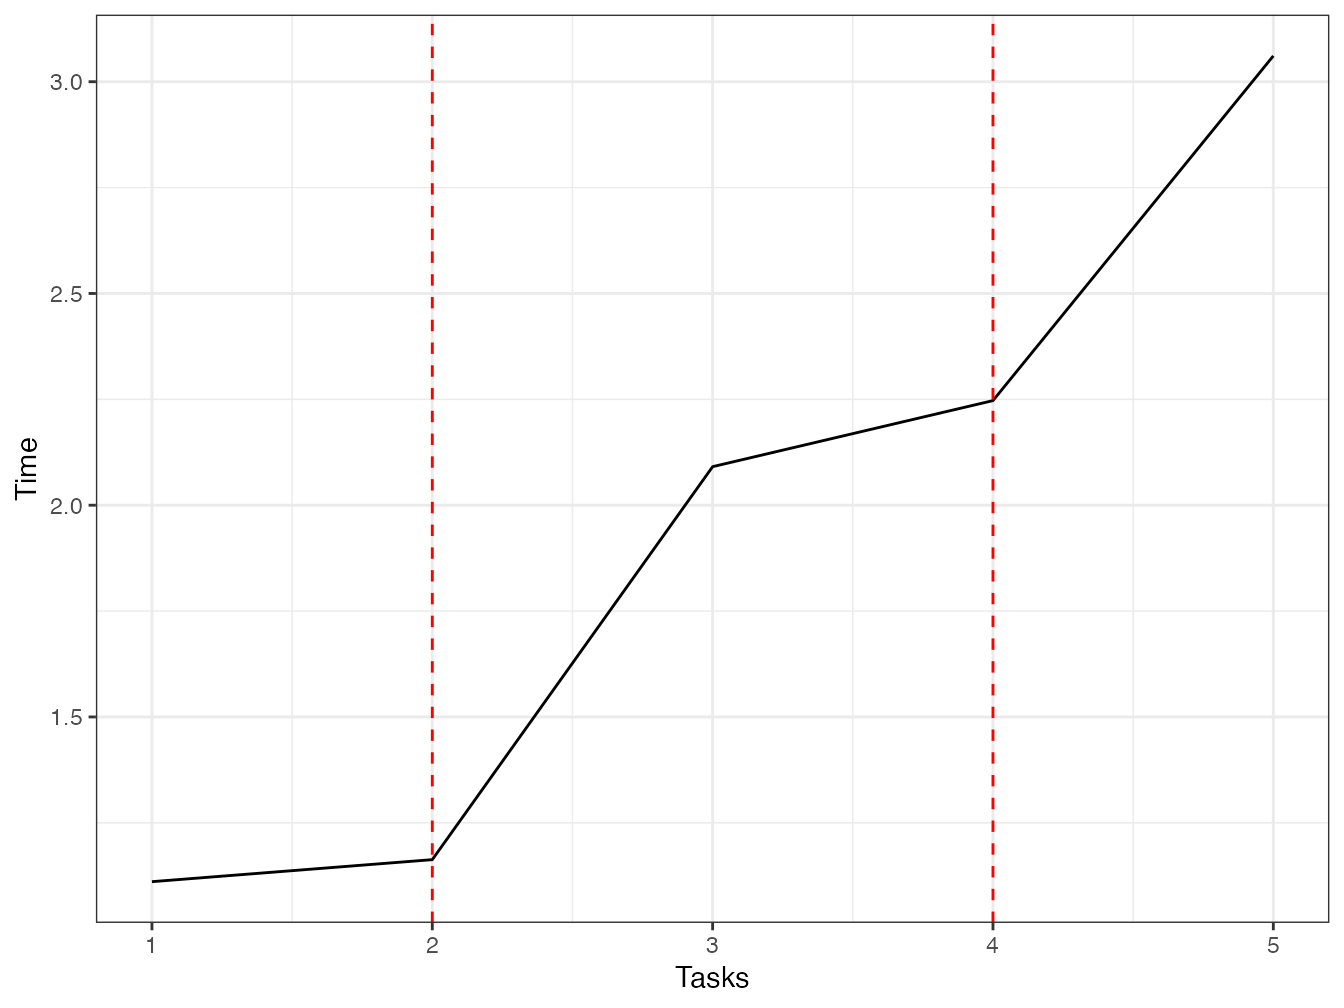
\includegraphics[width=0.8\linewidth]{WwR_files/figure-latex/r-parallele-1} 

}

\caption[Execution time in parallel]{Parallel execution time of tasks requiring one second (each task is a one second pause). The number of tasks varies from 1 to twice the number of cores used (equal to \texttt{2}) plus one.}\label{fig:r-parallele}
\end{figure}

\normalsize

The theoretical shape of this curve is as follows:

\begin{itemize}
\tightlist
\item
  For a task, the time is equal to one second plus the parallelization setup time.
\item
  The time should remain stable until the number of cores used.
\item
  When all the cores are used (red dotted line), the time should increase by one second and then remain stable until the next limit.
\end{itemize}

In practice, the computation time is determined by other factors that are difficult to predict.
The best practice is to adapt the number of tasks to the number of cores, otherwise performance will be lost.

\subsection{parLapply (socket)}\label{parlapply-socket}

\texttt{parLapply} requires to create a cluster, export the useful variables on each node, load the necessary packages on each node, execute the code and finally stop the cluster.
The code for each step can be found in the \texttt{mclapply.hack} function above.

For everyday use, \texttt{mclapply} is faster, except on Windows, and simpler (including on Windows thanks to the above workaround).

\subsection{foreach}\label{foreach}

\subsubsection{How it works}\label{how-it-works}

The \textbf{foreach} package allows advanced use of parallelization.
Read its vignettes.

\scriptsize

\begin{Shaded}
\begin{Highlighting}[]
\CommentTok{\# Manual}
\FunctionTok{vignette}\NormalTok{(}\StringTok{"foreach"}\NormalTok{, }\StringTok{"foreach"}\NormalTok{)}
\CommentTok{\# Nested loops}
\FunctionTok{vignette}\NormalTok{(}\StringTok{"nested"}\NormalTok{, }\StringTok{"foreach"}\NormalTok{)}
\end{Highlighting}
\end{Shaded}

\normalsize

Regardless of parallelization, \textbf{foreach} redefines \emph{for} loops.

\scriptsize

\begin{Shaded}
\begin{Highlighting}[]
\ControlFlowTok{for}\NormalTok{ (i }\ControlFlowTok{in} \DecValTok{1}\SpecialCharTok{:}\DecValTok{3}\NormalTok{) \{}
  \FunctionTok{f}\NormalTok{(i)}
\NormalTok{\}}
\CommentTok{\# becomes}
\FunctionTok{library}\NormalTok{(}\StringTok{"foreach"}\NormalTok{)}
\FunctionTok{foreach}\NormalTok{(}\AttributeTok{i =} \DecValTok{1}\SpecialCharTok{:}\DecValTok{3}\NormalTok{) }\SpecialCharTok{\%do\%}\NormalTok{ \{}
  \FunctionTok{f}\NormalTok{(i)}
\NormalTok{\}}
\end{Highlighting}
\end{Shaded}

\begin{verbatim}
## [[1]]
## [1] 1
## 
## [[2]]
## [1] 2
## 
## [[3]]
## [1] 3
\end{verbatim}

\normalsize

The \texttt{foreach} function returns a list containing the results of each loop.
The elements of the list can be combined by any function, such as \texttt{c}.

\scriptsize

\begin{Shaded}
\begin{Highlighting}[]
\FunctionTok{foreach}\NormalTok{(}\AttributeTok{i =} \DecValTok{1}\SpecialCharTok{:}\DecValTok{3}\NormalTok{, }\AttributeTok{.combine =} \StringTok{"c"}\NormalTok{) }\SpecialCharTok{\%do\%}\NormalTok{ \{}
  \FunctionTok{f}\NormalTok{(i)}
\NormalTok{\}}
\end{Highlighting}
\end{Shaded}

\begin{verbatim}
## [1] 1 2 3
\end{verbatim}

\normalsize

The \texttt{foreach} function is capable of using iterators, that is, functions that pass to the loop only the data it needs without loading the rest into memory.
Here, the \texttt{icount} iterator passes the values 1, 2 and 3 individually, without loading the 1:3 vector into memory.

\scriptsize

\begin{Shaded}
\begin{Highlighting}[]
\FunctionTok{library}\NormalTok{(}\StringTok{"iterators"}\NormalTok{)}
\FunctionTok{foreach}\NormalTok{(}\AttributeTok{i =} \FunctionTok{icount}\NormalTok{(}\DecValTok{3}\NormalTok{), }\AttributeTok{.combine =} \StringTok{"c"}\NormalTok{) }\SpecialCharTok{\%do\%}\NormalTok{ \{}
  \FunctionTok{f}\NormalTok{(i)}
\NormalTok{\}}
\end{Highlighting}
\end{Shaded}

\begin{verbatim}
## [1] 1 2 3
\end{verbatim}

\normalsize

It is therefore very useful when each object of the loop uses a large amount of memory.

\subsubsection{Parallelization}\label{parallelization}

Replacing the \texttt{\%do\%} operator with \texttt{\%dopar\%} parallelizes loops, provided that an adapter, i.e.~an intermediate package between \texttt{foreach} and a package implementing parallelization, is loaded.
\textbf{doParallel} is an adapter for using the \textbf{parallel} package that comes with R.

\scriptsize

\begin{Shaded}
\begin{Highlighting}[]
\FunctionTok{library}\NormalTok{(doParallel)}
\FunctionTok{registerDoParallel}\NormalTok{(}\AttributeTok{cores =}\NormalTok{ n\_cores)}
\CommentTok{\# Serial}
\FunctionTok{system.time}\NormalTok{(}
  \FunctionTok{foreach}\NormalTok{(}\AttributeTok{i =} \FunctionTok{icount}\NormalTok{(n\_cores), }\AttributeTok{.combine =} \StringTok{"c"}\NormalTok{) }\SpecialCharTok{\%do\%}\NormalTok{ \{}\FunctionTok{f}\NormalTok{(i)\}}
\NormalTok{)}
\end{Highlighting}
\end{Shaded}

\begin{verbatim}
##    user  system elapsed 
##   0.002   0.000   0.714
\end{verbatim}

\begin{Shaded}
\begin{Highlighting}[]
\CommentTok{\# Parallel}
\FunctionTok{system.time}\NormalTok{(}
  \FunctionTok{foreach}\NormalTok{(}\AttributeTok{i =} \FunctionTok{icount}\NormalTok{(n\_cores), }\AttributeTok{.combine =} \StringTok{"c"}\NormalTok{) }\SpecialCharTok{\%dopar\%}\NormalTok{ \{}\FunctionTok{f}\NormalTok{(i)\}}
\NormalTok{)}
\end{Highlighting}
\end{Shaded}

\begin{verbatim}
##    user  system elapsed 
##   0.005   0.032   0.359
\end{verbatim}

\normalsize

The fixed cost of parallelization is low.

\subsection{future}\label{future}

The \textbf{future} package is used to abstract the code of the parallelization implementation.
It is at the centre of an ecosystem of packages that facilitate its use\footnote{\url{https://www.futureverse.org/}}.

The parallelization strategy used is declared by the \texttt{plan()} function.
The default strategy is \texttt{sequential}, i.e.~single-task.
The \texttt{multicore} and \texttt{multisession} strategies are based respectively on the \emph{fork} and \emph{socket} techniques seen above.
Other strategies are available for using physical clusters (several computers prepared to run R together): the \textbf{future} documentation details how to do this.

Here we will use the \texttt{multisession} strategy, which works on the local computer, whatever its operating system.

\scriptsize

\begin{Shaded}
\begin{Highlighting}[]
\FunctionTok{library}\NormalTok{(}\StringTok{"future"}\NormalTok{)}
\CommentTok{\# Socket strategy on all available cores except 1}
\NormalTok{usedCores }\OtherTok{\textless{}{-}} \FunctionTok{availableCores}\NormalTok{(}\AttributeTok{omit =} \DecValTok{1}\NormalTok{)}
\FunctionTok{plan}\NormalTok{(multisession, }\AttributeTok{workers =}\NormalTok{ usedCores)}
\end{Highlighting}
\end{Shaded}

\normalsize

The \textbf{future.apply} package allows all \texttt{*apply()} and \texttt{replicate()} loops to be effortlessly parallelized by prefixing their names with \texttt{future\_}.

\scriptsize

\begin{Shaded}
\begin{Highlighting}[]
\FunctionTok{library}\NormalTok{(}\StringTok{"future.apply"}\NormalTok{)}
\FunctionTok{system.time}\NormalTok{(}\FunctionTok{future\_replicate}\NormalTok{(usedCores }\SpecialCharTok{{-}} \DecValTok{1}\NormalTok{, }\FunctionTok{f}\NormalTok{(usedCores)))}
\end{Highlighting}
\end{Shaded}

\begin{verbatim}
##    user  system elapsed 
##   0.021   0.001   0.313
\end{verbatim}

\normalsize

foreach loops can be parallelized with the \textbf{doFuture} package by simply replacing \texttt{\%dopar\%} with \texttt{\%dofuture\%}.

\scriptsize

\begin{Shaded}
\begin{Highlighting}[]
\FunctionTok{library}\NormalTok{(}\StringTok{"doFuture"}\NormalTok{)}
\FunctionTok{system.time}\NormalTok{(}
  \FunctionTok{foreach}\NormalTok{(}\AttributeTok{i =} \FunctionTok{icount}\NormalTok{(n\_cores), }\AttributeTok{.combine =} \StringTok{"c"}\NormalTok{) }\SpecialCharTok{\%dofuture\%}\NormalTok{ \{}\FunctionTok{f}\NormalTok{(i)\}}
\NormalTok{)}
\end{Highlighting}
\end{Shaded}

\begin{verbatim}
##    user  system elapsed 
##   0.042   0.002   0.559
\end{verbatim}

\normalsize

The strategy is reset to \texttt{sequential} at the end.

\scriptsize

\begin{Shaded}
\begin{Highlighting}[]
\FunctionTok{plan}\NormalTok{(sequential)}
\end{Highlighting}
\end{Shaded}

\normalsize

\section{Case study}\label{sec:cas}

This case study tests the different techniques seen above to solve a concrete problem.
The objective is to compute the average distance between two points of a random set of 1000 points in a square window of side 1.

Its expectation is computable\footnote{\url{https://mindyourdecisions.com/blog/2016/07/03/distance-between-two-random-points-in-a-square-sunday-puzzle/}}.
It is equal to \(\frac{2+\sqrt{2}+5\ln{(1+\sqrt{2})}}{15} \approx 0.5214\).

\subsection{Creation of the data}\label{creation-of-the-data}

The point set is created with the \textbf{spatstat} package.

\scriptsize

\begin{Shaded}
\begin{Highlighting}[]
\NormalTok{n\_points }\OtherTok{\textless{}{-}} \DecValTok{1000}
\FunctionTok{library}\NormalTok{(}\StringTok{"spatstat"}\NormalTok{)}
\NormalTok{X }\OtherTok{\textless{}{-}} \FunctionTok{runifpoint}\NormalTok{(n\_points)}
\end{Highlighting}
\end{Shaded}

\normalsize

\subsection{Spatstat}\label{spatstat}

The \texttt{pairdist()} function of \textbf{spatstat} returns the matrix of distances between points.
The average distance is calculated by dividing the sum by the number of pairs of distinct points.

\scriptsize

\begin{Shaded}
\begin{Highlighting}[]
\NormalTok{mb }\OtherTok{\textless{}{-}} \FunctionTok{microbenchmark}\NormalTok{(d }\OtherTok{\textless{}{-}} \FunctionTok{sum}\NormalTok{(}\FunctionTok{pairdist}\NormalTok{(X)) }\SpecialCharTok{/}\NormalTok{ n\_points }\SpecialCharTok{/}\NormalTok{ (n\_points }\SpecialCharTok{{-}} \DecValTok{1}\NormalTok{))}
\FunctionTok{autoplot}\NormalTok{(mb)}
\end{Highlighting}
\end{Shaded}

\begin{center}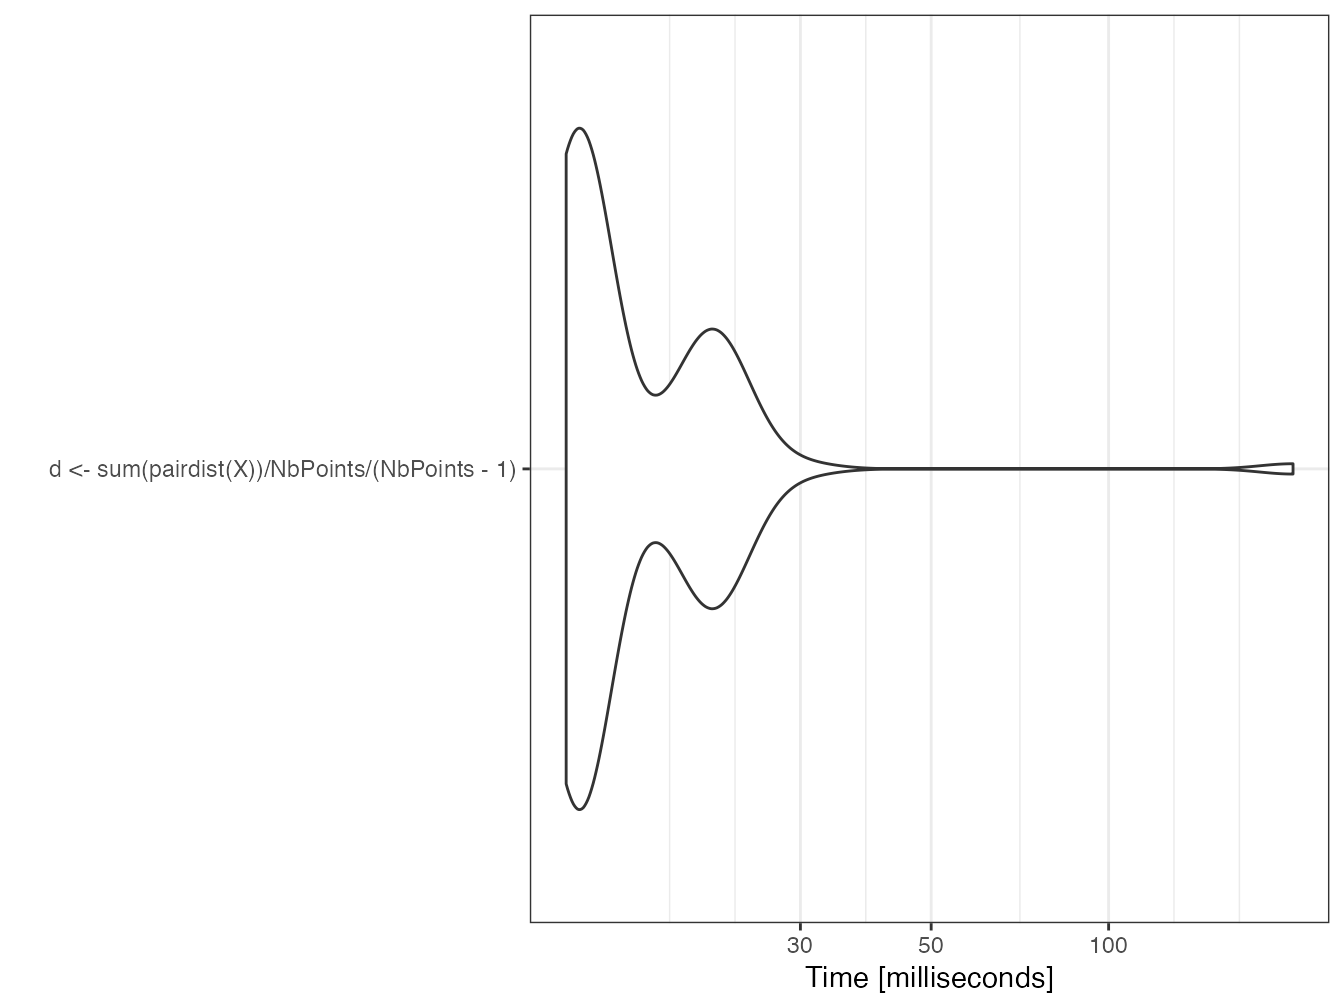
\includegraphics[width=0.8\linewidth]{WwR_files/figure-latex/pairdist-1} \end{center}

\begin{Shaded}
\begin{Highlighting}[]
\NormalTok{d}
\end{Highlighting}
\end{Shaded}

\begin{verbatim}
## [1] 0.5154879
\end{verbatim}

\normalsize

The function is fast because it is coded in C in the \textbf{spatstat} package for the core of its calculations.

\subsection{apply}\label{apply}

The distance can be calculated by two nested \texttt{sapply()}.

\scriptsize

\begin{Shaded}
\begin{Highlighting}[]
\NormalTok{fsapply1 }\OtherTok{\textless{}{-}} \ControlFlowTok{function}\NormalTok{() \{}
\NormalTok{  distances }\OtherTok{\textless{}{-}} \FunctionTok{sapply}\NormalTok{(}
    \DecValTok{1}\SpecialCharTok{:}\NormalTok{n\_points, }
    \AttributeTok{FUN =} \ControlFlowTok{function}\NormalTok{(i) \{}
      \FunctionTok{sapply}\NormalTok{(}
        \DecValTok{1}\SpecialCharTok{:}\NormalTok{n\_points, }
        \AttributeTok{FUN =} \ControlFlowTok{function}\NormalTok{(j) \{}
          \FunctionTok{sqrt}\NormalTok{((X}\SpecialCharTok{$}\NormalTok{x[i] }\SpecialCharTok{{-}}\NormalTok{ X}\SpecialCharTok{$}\NormalTok{x[j])}\SpecialCharTok{\^{}}\DecValTok{2} \SpecialCharTok{+}\NormalTok{ (X}\SpecialCharTok{$}\NormalTok{y[i] }\SpecialCharTok{{-}}\NormalTok{ X}\SpecialCharTok{$}\NormalTok{y[j])}\SpecialCharTok{\^{}}\DecValTok{2}\NormalTok{)}
\NormalTok{        \}}
\NormalTok{      )}
\NormalTok{    \} }
\NormalTok{  )}
  \FunctionTok{return}\NormalTok{(}\FunctionTok{sum}\NormalTok{(distances) }\SpecialCharTok{/}\NormalTok{ n\_points }\SpecialCharTok{/}\NormalTok{ (n\_points }\SpecialCharTok{{-}} \DecValTok{1}\NormalTok{))}
\NormalTok{\}}
\FunctionTok{system.time}\NormalTok{(d }\OtherTok{\textless{}{-}} \FunctionTok{fsapply1}\NormalTok{())}
\end{Highlighting}
\end{Shaded}

\begin{verbatim}
##    user  system elapsed 
##   3.150   0.064   3.267
\end{verbatim}

\begin{Shaded}
\begin{Highlighting}[]
\NormalTok{d}
\end{Highlighting}
\end{Shaded}

\begin{verbatim}
## [1] 0.5154879
\end{verbatim}

\normalsize

Some time can be saved by replacing \texttt{sapply} with \texttt{vapply}: the format of the results does not have to be determined by the function.
The gain is negligible on a long computation like this one but important for short computations.

\scriptsize

\begin{Shaded}
\begin{Highlighting}[]
\NormalTok{fsapply2 }\OtherTok{\textless{}{-}} \ControlFlowTok{function}\NormalTok{() \{}
\NormalTok{  distances }\OtherTok{\textless{}{-}} \FunctionTok{vapply}\NormalTok{(}
    \DecValTok{1}\SpecialCharTok{:}\NormalTok{n\_points, }
    \AttributeTok{FUN =} \ControlFlowTok{function}\NormalTok{(i) \{}
      \FunctionTok{vapply}\NormalTok{(}
        \DecValTok{1}\SpecialCharTok{:}\NormalTok{n\_points, }
        \AttributeTok{FUN =} \ControlFlowTok{function}\NormalTok{(j) \{}
          \FunctionTok{sqrt}\NormalTok{((X}\SpecialCharTok{$}\NormalTok{x[i] }\SpecialCharTok{{-}}\NormalTok{ X}\SpecialCharTok{$}\NormalTok{x[j])}\SpecialCharTok{\^{}}\DecValTok{2} \SpecialCharTok{+}\NormalTok{ (X}\SpecialCharTok{$}\NormalTok{y[i] }\SpecialCharTok{{-}}\NormalTok{ X}\SpecialCharTok{$}\NormalTok{y[j])}\SpecialCharTok{\^{}}\DecValTok{2}\NormalTok{)}
\NormalTok{        \}, }
        \AttributeTok{FUN.VALUE =} \DecValTok{0}
\NormalTok{      )}
\NormalTok{    \}, }
    \AttributeTok{FUN.VALUE =} \DecValTok{1}\SpecialCharTok{:}\DecValTok{1000} \SpecialCharTok{+} \DecValTok{0}
\NormalTok{  )}
  \FunctionTok{return}\NormalTok{(}\FunctionTok{sum}\NormalTok{(distances) }\SpecialCharTok{/}\NormalTok{ n\_points }\SpecialCharTok{/}\NormalTok{ (n\_points }\SpecialCharTok{{-}} \DecValTok{1}\NormalTok{))}
\NormalTok{\}}
\FunctionTok{system.time}\NormalTok{(d }\OtherTok{\textless{}{-}} \FunctionTok{fsapply2}\NormalTok{())}
\end{Highlighting}
\end{Shaded}

\begin{verbatim}
##    user  system elapsed 
##   2.666   0.049   2.781
\end{verbatim}

\begin{Shaded}
\begin{Highlighting}[]
\NormalTok{d}
\end{Highlighting}
\end{Shaded}

\begin{verbatim}
## [1] 0.5154879
\end{verbatim}

\normalsize

The output format is not always obvious to write:

\begin{itemize}
\tightlist
\item
  it must respect the size of the data: a vector of size 1000 for the outer loop, a scalar for the inner loop.
\item
  it must respect the type: \texttt{0L} for an integer, \texttt{0} for a real number. In the outer loop, adding \texttt{0} to the vector of integers turns it into a vector of real numbers.
\end{itemize}

A more significant improvement is to compute the square roots only at the end of the loop, to take advantage of the vectorization of the function.

\scriptsize

\begin{Shaded}
\begin{Highlighting}[]
\NormalTok{fsapply3 }\OtherTok{\textless{}{-}} \ControlFlowTok{function}\NormalTok{() \{}
\NormalTok{  distances }\OtherTok{\textless{}{-}} \FunctionTok{vapply}\NormalTok{(}
    \DecValTok{1}\SpecialCharTok{:}\NormalTok{n\_points, }
    \AttributeTok{FUN =} \ControlFlowTok{function}\NormalTok{(i) \{}
      \FunctionTok{vapply}\NormalTok{(}
        \DecValTok{1}\SpecialCharTok{:}\NormalTok{n\_points, }
        \AttributeTok{FUN =} \ControlFlowTok{function}\NormalTok{(j) \{}
\NormalTok{          (X}\SpecialCharTok{$}\NormalTok{x[i] }\SpecialCharTok{{-}}\NormalTok{ X}\SpecialCharTok{$}\NormalTok{x[j])}\SpecialCharTok{\^{}}\DecValTok{2} \SpecialCharTok{+}\NormalTok{ (X}\SpecialCharTok{$}\NormalTok{y[i] }\SpecialCharTok{{-}}\NormalTok{ X}\SpecialCharTok{$}\NormalTok{y[j])}\SpecialCharTok{\^{}}\DecValTok{2}
\NormalTok{        \}, }
        \AttributeTok{FUN.VALUE =} \DecValTok{0}
\NormalTok{      )}
\NormalTok{    \}, }
    \AttributeTok{FUN.VALUE =} \DecValTok{1}\SpecialCharTok{:}\DecValTok{1000} \SpecialCharTok{+} \DecValTok{0}
\NormalTok{  )}
  \FunctionTok{return}\NormalTok{(}\FunctionTok{sum}\NormalTok{(}\FunctionTok{sqrt}\NormalTok{(distances)) }\SpecialCharTok{/}\NormalTok{ n\_points }\SpecialCharTok{/}\NormalTok{ (n\_points }\SpecialCharTok{{-}} \DecValTok{1}\NormalTok{))}
\NormalTok{\}}
\FunctionTok{system.time}\NormalTok{(d }\OtherTok{\textless{}{-}} \FunctionTok{fsapply3}\NormalTok{())}
\end{Highlighting}
\end{Shaded}

\begin{verbatim}
##    user  system elapsed 
##   2.654   0.039   2.724
\end{verbatim}

\begin{Shaded}
\begin{Highlighting}[]
\NormalTok{d}
\end{Highlighting}
\end{Shaded}

\begin{verbatim}
## [1] 0.5154879
\end{verbatim}

\normalsize

The computations are performed twice (distance between points \(i\) and \(j\), but also between points \(j\) and \(i\)): a test on the indices allows to divide the time almost by 2 (not quite because the loops without computation, which return \(0\), take time).

\scriptsize

\begin{Shaded}
\begin{Highlighting}[]
\NormalTok{fsapply4 }\OtherTok{\textless{}{-}} \ControlFlowTok{function}\NormalTok{() \{}
\NormalTok{  distances }\OtherTok{\textless{}{-}} \FunctionTok{vapply}\NormalTok{(}
    \DecValTok{1}\SpecialCharTok{:}\NormalTok{n\_points, }
    \AttributeTok{FUN =} \ControlFlowTok{function}\NormalTok{(i) \{}
      \FunctionTok{vapply}\NormalTok{(}
        \DecValTok{1}\SpecialCharTok{:}\NormalTok{n\_points, }
        \AttributeTok{FUN =} \ControlFlowTok{function}\NormalTok{(j) \{}
          \ControlFlowTok{if}\NormalTok{ (j }\SpecialCharTok{\textgreater{}}\NormalTok{ i) \{}
\NormalTok{            (X}\SpecialCharTok{$}\NormalTok{x[i] }\SpecialCharTok{{-}}\NormalTok{ X}\SpecialCharTok{$}\NormalTok{x[j])}\SpecialCharTok{\^{}}\DecValTok{2} \SpecialCharTok{+}\NormalTok{ (X}\SpecialCharTok{$}\NormalTok{y[i] }\SpecialCharTok{{-}}\NormalTok{ X}\SpecialCharTok{$}\NormalTok{y[j])}\SpecialCharTok{\^{}}\DecValTok{2}
\NormalTok{          \} }\ControlFlowTok{else}\NormalTok{ \{}
            \DecValTok{0}
\NormalTok{          \}}
\NormalTok{        \}, }
        \AttributeTok{FUN.VALUE =} \DecValTok{0}
\NormalTok{      )}
\NormalTok{    \}, }
    \AttributeTok{FUN.VALUE =} \DecValTok{1}\SpecialCharTok{:}\DecValTok{1000} \SpecialCharTok{+} \DecValTok{0}
\NormalTok{  )}
  \FunctionTok{return}\NormalTok{(}\FunctionTok{sum}\NormalTok{(}\FunctionTok{sqrt}\NormalTok{(distances)) }\SpecialCharTok{/}\NormalTok{ n\_points }\SpecialCharTok{/}\NormalTok{ (n\_points }\SpecialCharTok{{-}} \DecValTok{1}\NormalTok{) }\SpecialCharTok{*} \DecValTok{2}\NormalTok{)}
\NormalTok{\}}
\FunctionTok{system.time}\NormalTok{(d }\OtherTok{\textless{}{-}} \FunctionTok{fsapply4}\NormalTok{())}
\end{Highlighting}
\end{Shaded}

\begin{verbatim}
##    user  system elapsed 
##   1.611   0.024   1.652
\end{verbatim}

\begin{Shaded}
\begin{Highlighting}[]
\NormalTok{d}
\end{Highlighting}
\end{Shaded}

\begin{verbatim}
## [1] 0.5154879
\end{verbatim}

\normalsize

In parallel, the computation time is not improved on Windows because the individual tasks are too short.
On MacOS or Linux, the computation is accelerated.

\scriptsize

\begin{Shaded}
\begin{Highlighting}[]
\NormalTok{fsapply5 }\OtherTok{\textless{}{-}} \ControlFlowTok{function}\NormalTok{() \{}
\NormalTok{  distances }\OtherTok{\textless{}{-}} \FunctionTok{mclapply}\NormalTok{(}
    \DecValTok{1}\SpecialCharTok{:}\NormalTok{n\_points, }
    \CommentTok{\# Avoid naming the argument because it is named FUN in mclapply()}
    \CommentTok{\# but fun in parLapply() used by  mclapply.hack()}
    \ControlFlowTok{function}\NormalTok{(i) \{}
      \FunctionTok{vapply}\NormalTok{(}
        \DecValTok{1}\SpecialCharTok{:}\NormalTok{n\_points, }
        \AttributeTok{FUN =} \ControlFlowTok{function}\NormalTok{(j) \{}
          \ControlFlowTok{if}\NormalTok{ (j }\SpecialCharTok{\textgreater{}}\NormalTok{ i) \{}
\NormalTok{            (X}\SpecialCharTok{$}\NormalTok{x[i] }\SpecialCharTok{{-}}\NormalTok{ X}\SpecialCharTok{$}\NormalTok{x[j])}\SpecialCharTok{\^{}}\DecValTok{2} \SpecialCharTok{+}\NormalTok{ (X}\SpecialCharTok{$}\NormalTok{y[i] }\SpecialCharTok{{-}}\NormalTok{ X}\SpecialCharTok{$}\NormalTok{y[j])}\SpecialCharTok{\^{}}\DecValTok{2}
\NormalTok{          \} }\ControlFlowTok{else}\NormalTok{ \{}
            \DecValTok{0}
\NormalTok{          \}}
\NormalTok{        \},}
        \AttributeTok{FUN.VALUE =} \DecValTok{0}
\NormalTok{      )}
\NormalTok{    \}}
\NormalTok{  )}
  \FunctionTok{return}\NormalTok{(}
    \FunctionTok{sum}\NormalTok{(}\FunctionTok{sqrt}\NormalTok{(}\FunctionTok{simplify2array}\NormalTok{(distances))) }\SpecialCharTok{/}\NormalTok{ n\_points }\SpecialCharTok{/}\NormalTok{ (n\_points }\SpecialCharTok{{-}} \DecValTok{1}\NormalTok{) }\SpecialCharTok{*} \DecValTok{2}
\NormalTok{  )}
\NormalTok{\}}
\FunctionTok{system.time}\NormalTok{(d }\OtherTok{\textless{}{-}} \FunctionTok{fsapply5}\NormalTok{())}
\end{Highlighting}
\end{Shaded}

\begin{verbatim}
##    user  system elapsed 
##   1.995   0.434   1.397
\end{verbatim}

\begin{Shaded}
\begin{Highlighting}[]
\NormalTok{d}
\end{Highlighting}
\end{Shaded}

\begin{verbatim}
## [1] 0.5154879
\end{verbatim}

\normalsize

\subsection{future.apply}\label{future.apply}

The \texttt{fsapply4()} function optimised above can be parallelled directly by prefixing the \texttt{vapply} function with \texttt{future\_}.
Only the main loop is parallelized: nesting \texttt{future\_vapply()} would collapse performance.

\scriptsize

\begin{Shaded}
\begin{Highlighting}[]
\FunctionTok{library}\NormalTok{(}\StringTok{"future.apply"}\NormalTok{)}
\CommentTok{\# Socket strategy on all available cores except 1}
\FunctionTok{plan}\NormalTok{(multisession, }\AttributeTok{workers =} \FunctionTok{availableCores}\NormalTok{(}\AttributeTok{omit =} \DecValTok{1}\NormalTok{))}
\NormalTok{future\_fsapply4\_ }\OtherTok{\textless{}{-}} \ControlFlowTok{function}\NormalTok{() \{}
\NormalTok{  distances }\OtherTok{\textless{}{-}} \FunctionTok{future\_vapply}\NormalTok{(}
    \DecValTok{1}\SpecialCharTok{:}\NormalTok{n\_points, }
    \AttributeTok{FUN =} \ControlFlowTok{function}\NormalTok{(i) \{}
      \FunctionTok{vapply}\NormalTok{(}
        \DecValTok{1}\SpecialCharTok{:}\NormalTok{n\_points, }
        \AttributeTok{FUN =} \ControlFlowTok{function}\NormalTok{(j) \{}
          \ControlFlowTok{if}\NormalTok{ (j }\SpecialCharTok{\textgreater{}}\NormalTok{ i) \{}
\NormalTok{            (X}\SpecialCharTok{$}\NormalTok{x[i] }\SpecialCharTok{{-}}\NormalTok{ X}\SpecialCharTok{$}\NormalTok{x[j])}\SpecialCharTok{\^{}}\DecValTok{2} \SpecialCharTok{+}\NormalTok{ (X}\SpecialCharTok{$}\NormalTok{y[i] }\SpecialCharTok{{-}}\NormalTok{ X}\SpecialCharTok{$}\NormalTok{y[j])}\SpecialCharTok{\^{}}\DecValTok{2}
\NormalTok{          \} }\ControlFlowTok{else}\NormalTok{ \{}
            \DecValTok{0}
\NormalTok{          \}}
\NormalTok{        \}, }
        \AttributeTok{FUN.VALUE =} \DecValTok{0}
\NormalTok{      )}
\NormalTok{    \}, }
    \AttributeTok{FUN.VALUE =} \DecValTok{1}\SpecialCharTok{:}\DecValTok{1000} \SpecialCharTok{+} \DecValTok{0}
\NormalTok{  )}
  \FunctionTok{return}\NormalTok{(}\FunctionTok{sum}\NormalTok{(}\FunctionTok{sqrt}\NormalTok{(distances)) }\SpecialCharTok{/}\NormalTok{ n\_points }\SpecialCharTok{/}\NormalTok{ (n\_points }\SpecialCharTok{{-}} \DecValTok{1}\NormalTok{) }\SpecialCharTok{*} \DecValTok{2}\NormalTok{)}
\NormalTok{\}}
\FunctionTok{system.time}\NormalTok{(d }\OtherTok{\textless{}{-}} \FunctionTok{future\_fsapply4\_}\NormalTok{())}
\end{Highlighting}
\end{Shaded}

\begin{verbatim}
##    user  system elapsed 
##   0.059   0.009   1.224
\end{verbatim}

\begin{Shaded}
\begin{Highlighting}[]
\NormalTok{d}
\end{Highlighting}
\end{Shaded}

\begin{verbatim}
## [1] 0.5154879
\end{verbatim}

\begin{Shaded}
\begin{Highlighting}[]
\FunctionTok{plan}\NormalTok{(sequential)}
\end{Highlighting}
\end{Shaded}

\normalsize

\subsection{for loop}\label{for-loop}

A for loop is faster and consumes less memory because it does not store the distance matrix.

\scriptsize

\begin{Shaded}
\begin{Highlighting}[]
\NormalTok{distance }\OtherTok{\textless{}{-}} \DecValTok{0}
\NormalTok{ffor }\OtherTok{\textless{}{-}} \ControlFlowTok{function}\NormalTok{() \{}
  \ControlFlowTok{for}\NormalTok{ (i }\ControlFlowTok{in} \DecValTok{1}\SpecialCharTok{:}\NormalTok{(n\_points }\SpecialCharTok{{-}} \DecValTok{1}\NormalTok{)) \{}
    \ControlFlowTok{for}\NormalTok{ (j }\ControlFlowTok{in}\NormalTok{ (i }\SpecialCharTok{+} \DecValTok{1}\NormalTok{)}\SpecialCharTok{:}\NormalTok{n\_points) \{}
\NormalTok{      distance }\OtherTok{\textless{}{-}}\NormalTok{ distance }\SpecialCharTok{+} \FunctionTok{sqrt}\NormalTok{((X}\SpecialCharTok{$}\NormalTok{x[i] }\SpecialCharTok{{-}}\NormalTok{ X}\SpecialCharTok{$}\NormalTok{x[j])}\SpecialCharTok{\^{}}\DecValTok{2} \SpecialCharTok{+}\NormalTok{ (X}\SpecialCharTok{$}\NormalTok{y[i] }\SpecialCharTok{{-}}\NormalTok{ X}\SpecialCharTok{$}\NormalTok{y[j])}\SpecialCharTok{\^{}}\DecValTok{2}\NormalTok{)}
\NormalTok{    \}}
\NormalTok{  \}}
  \FunctionTok{return}\NormalTok{(distance }\SpecialCharTok{/}\NormalTok{ n\_points }\SpecialCharTok{/}\NormalTok{ (n\_points }\SpecialCharTok{{-}} \DecValTok{1}\NormalTok{) }\SpecialCharTok{*} \DecValTok{2}\NormalTok{)}
\NormalTok{\}}
\CommentTok{\# Calculation time, stored}
\NormalTok{(for\_time }\OtherTok{\textless{}{-}} \FunctionTok{system.time}\NormalTok{(d }\OtherTok{\textless{}{-}} \FunctionTok{ffor}\NormalTok{()))}
\end{Highlighting}
\end{Shaded}

\begin{verbatim}
##    user  system elapsed 
##   0.916   0.010   0.927
\end{verbatim}

\begin{Shaded}
\begin{Highlighting}[]
\NormalTok{d}
\end{Highlighting}
\end{Shaded}

\begin{verbatim}
## [1] 0.5154879
\end{verbatim}

\normalsize

This is the simplest and most efficient way to write this code with core R and no parallelization.

\subsection{foreach loop}\label{foreach-loop}

Parallelization executes for loops inside a foreach loop, which is quite efficient.
However, distances are calculated twice.

\scriptsize

\begin{Shaded}
\begin{Highlighting}[]
\FunctionTok{registerDoParallel}\NormalTok{(}\AttributeTok{cores =} \FunctionTok{detectCores}\NormalTok{())}
\NormalTok{fforeach3 }\OtherTok{\textless{}{-}} \ControlFlowTok{function}\NormalTok{(Y) \{}
\NormalTok{  distances }\OtherTok{\textless{}{-}} \FunctionTok{foreach}\NormalTok{(}\AttributeTok{i =} \FunctionTok{icount}\NormalTok{(Y}\SpecialCharTok{$}\NormalTok{n), }\AttributeTok{.combine =} \StringTok{\textquotesingle{}+\textquotesingle{}}\NormalTok{) }\SpecialCharTok{\%dopar\%}\NormalTok{ \{}
\NormalTok{    distance }\OtherTok{\textless{}{-}} \DecValTok{0}
    \ControlFlowTok{for}\NormalTok{ (j }\ControlFlowTok{in} \DecValTok{1}\SpecialCharTok{:}\NormalTok{Y}\SpecialCharTok{$}\NormalTok{n) \{}
\NormalTok{      distance }\OtherTok{\textless{}{-}}\NormalTok{ distance }\SpecialCharTok{+} \FunctionTok{sqrt}\NormalTok{((Y}\SpecialCharTok{$}\NormalTok{x[i] }\SpecialCharTok{{-}}\NormalTok{ Y}\SpecialCharTok{$}\NormalTok{x[j])}\SpecialCharTok{\^{}}\DecValTok{2} \SpecialCharTok{+}\NormalTok{ (Y}\SpecialCharTok{$}\NormalTok{y[i] }\SpecialCharTok{{-}}\NormalTok{ Y}\SpecialCharTok{$}\NormalTok{y[j])}\SpecialCharTok{\^{}}\DecValTok{2}\NormalTok{)}
\NormalTok{    \}}
\NormalTok{    distance}
\NormalTok{  \}}
  \FunctionTok{return}\NormalTok{(distances }\SpecialCharTok{/}\NormalTok{ Y}\SpecialCharTok{$}\NormalTok{n }\SpecialCharTok{/}\NormalTok{ (Y}\SpecialCharTok{$}\NormalTok{n }\SpecialCharTok{{-}} \DecValTok{1}\NormalTok{))}
\NormalTok{\}}
\FunctionTok{system.time}\NormalTok{(d }\OtherTok{\textless{}{-}} \FunctionTok{fforeach3}\NormalTok{(X))}
\end{Highlighting}
\end{Shaded}

\begin{verbatim}
##    user  system elapsed 
##   2.366   0.301   1.259
\end{verbatim}

\begin{Shaded}
\begin{Highlighting}[]
\NormalTok{d}
\end{Highlighting}
\end{Shaded}

\begin{verbatim}
## [1] 0.5154879
\end{verbatim}

\normalsize

It is possible to nest two foreach loops, but they are extremely slow compared with a simple loop.
The test is run here with 10 times fewer points, so 100 times fewer distances to calculate.

\scriptsize

\begin{Shaded}
\begin{Highlighting}[]
\NormalTok{n\_points\_reduced }\OtherTok{\textless{}{-}} \DecValTok{100}
\NormalTok{Y }\OtherTok{\textless{}{-}} \FunctionTok{runifpoint}\NormalTok{(n\_points\_reduced)}
\NormalTok{fforeach1 }\OtherTok{\textless{}{-}} \ControlFlowTok{function}\NormalTok{(Y) \{}
\NormalTok{  distances }\OtherTok{\textless{}{-}} \FunctionTok{foreach}\NormalTok{(}\AttributeTok{i =} \DecValTok{1}\SpecialCharTok{:}\NormalTok{n\_points\_reduced, }\AttributeTok{.combine =} \StringTok{\textquotesingle{}cbind\textquotesingle{}}\NormalTok{) }\SpecialCharTok{\%:\%}
    \FunctionTok{foreach}\NormalTok{(}\AttributeTok{j =} \DecValTok{1}\SpecialCharTok{:}\NormalTok{n\_points\_reduced, }\AttributeTok{.combine =} \StringTok{\textquotesingle{}c\textquotesingle{}}\NormalTok{) }\SpecialCharTok{\%do\%}\NormalTok{ \{}
      \ControlFlowTok{if}\NormalTok{ (j }\SpecialCharTok{\textgreater{}}\NormalTok{ i) \{}
\NormalTok{        (Y}\SpecialCharTok{$}\NormalTok{x[i] }\SpecialCharTok{{-}}\NormalTok{ Y}\SpecialCharTok{$}\NormalTok{x[j])}\SpecialCharTok{\^{}}\DecValTok{2} \SpecialCharTok{+}\NormalTok{ (Y}\SpecialCharTok{$}\NormalTok{y[i] }\SpecialCharTok{{-}}\NormalTok{ Y}\SpecialCharTok{$}\NormalTok{y[j])}\SpecialCharTok{\^{}}\DecValTok{2}
\NormalTok{      \} }\ControlFlowTok{else}\NormalTok{ \{}
        \DecValTok{0}
\NormalTok{      \}}
\NormalTok{    \}}
  \FunctionTok{return}\NormalTok{(}\FunctionTok{sum}\NormalTok{(}\FunctionTok{sqrt}\NormalTok{(distances)) }\SpecialCharTok{/}\NormalTok{ n\_points\_reduced }\SpecialCharTok{/}\NormalTok{ (n\_points\_reduced }\SpecialCharTok{{-}} \DecValTok{1}\NormalTok{) }\SpecialCharTok{*} \DecValTok{2}\NormalTok{)}
\NormalTok{\}}
\FunctionTok{system.time}\NormalTok{(d }\OtherTok{\textless{}{-}} \FunctionTok{fforeach1}\NormalTok{(Y))}
\end{Highlighting}
\end{Shaded}

\begin{verbatim}
##    user  system elapsed 
##   0.836   0.006   0.842
\end{verbatim}

\begin{Shaded}
\begin{Highlighting}[]
\NormalTok{d}
\end{Highlighting}
\end{Shaded}

\begin{verbatim}
## [1] 0.5304197
\end{verbatim}

\normalsize

Nested foreach loops should be reserved for very long tasks (several seconds at least) to compensate the fixed costs of setting them up.

\subsection{RCpp}\label{rcpp}

The C++ function to calculate distances is the following.

\scriptsize

\begin{Shaded}
\begin{Highlighting}[]
\PreprocessorTok{\#include }\ImportTok{\textless{}Rcpp.h\textgreater{}}
\KeywordTok{using} \KeywordTok{namespace}\NormalTok{ Rcpp}\OperatorTok{;}

\CommentTok{// [[Rcpp::export]]}
\DataTypeTok{double}\NormalTok{ MeanDistance}\OperatorTok{(}\NormalTok{NumericVector x}\OperatorTok{,}\NormalTok{ NumericVector y}\OperatorTok{)} \OperatorTok{\{}
  \DataTypeTok{double}\NormalTok{ distance }\OperatorTok{=} \DecValTok{0}\OperatorTok{;}
  \DataTypeTok{double}\NormalTok{ dx}\OperatorTok{,}\NormalTok{ dy}\OperatorTok{;}
  \ControlFlowTok{for} \OperatorTok{(}\DataTypeTok{int}\NormalTok{ i }\OperatorTok{=} \DecValTok{0}\OperatorTok{;}\NormalTok{ i }\OperatorTok{\textless{}} \OperatorTok{(}\NormalTok{x}\OperatorTok{.}\NormalTok{length}\OperatorTok{()} \OperatorTok{{-}} \DecValTok{1}\OperatorTok{);}\NormalTok{ i}\OperatorTok{++)} \OperatorTok{\{}
    \ControlFlowTok{for} \OperatorTok{(}\DataTypeTok{int}\NormalTok{ j }\OperatorTok{=}\NormalTok{ i }\OperatorTok{+} \DecValTok{1}\OperatorTok{;}\NormalTok{ j }\OperatorTok{\textless{}}\NormalTok{ x}\OperatorTok{.}\NormalTok{length}\OperatorTok{();}\NormalTok{ j}\OperatorTok{++)} \OperatorTok{\{}
    \CommentTok{// Calculate distance}
\NormalTok{        dx }\OperatorTok{=}\NormalTok{ x}\OperatorTok{[}\NormalTok{i}\OperatorTok{]} \OperatorTok{{-}}\NormalTok{ x}\OperatorTok{[}\NormalTok{j}\OperatorTok{];}
\NormalTok{        dy }\OperatorTok{=}\NormalTok{ y}\OperatorTok{[}\NormalTok{i}\OperatorTok{]} \OperatorTok{{-}}\NormalTok{ y}\OperatorTok{[}\NormalTok{j}\OperatorTok{];}
\NormalTok{        distance }\OperatorTok{+=}\NormalTok{ sqrt}\OperatorTok{(}\NormalTok{dx }\OperatorTok{*}\NormalTok{ dx }\OperatorTok{+}\NormalTok{ dy }\OperatorTok{*}\NormalTok{ dy}\OperatorTok{);}
    \OperatorTok{\}}
  \OperatorTok{\}}
  \ControlFlowTok{return}\NormalTok{ distance }\OperatorTok{/} \OperatorTok{(}\DataTypeTok{double}\OperatorTok{)(}\NormalTok{x}\OperatorTok{.}\NormalTok{length}\OperatorTok{()} \OperatorTok{/} \DecValTok{2} \OperatorTok{*} \OperatorTok{(}\NormalTok{x}\OperatorTok{.}\NormalTok{length}\OperatorTok{()} \OperatorTok{{-}} \DecValTok{1}\OperatorTok{));}
\OperatorTok{\}}
\end{Highlighting}
\end{Shaded}

\normalsize

It is called in R very simply.
The computation time is very short.

\scriptsize

\begin{Shaded}
\begin{Highlighting}[]
\NormalTok{mb }\OtherTok{\textless{}{-}} \FunctionTok{microbenchmark}\NormalTok{(d }\OtherTok{\textless{}{-}} \FunctionTok{MeanDistance}\NormalTok{(X}\SpecialCharTok{$}\NormalTok{x, X}\SpecialCharTok{$}\NormalTok{y))}
\FunctionTok{autoplot}\NormalTok{(mb)}
\end{Highlighting}
\end{Shaded}

\begin{center}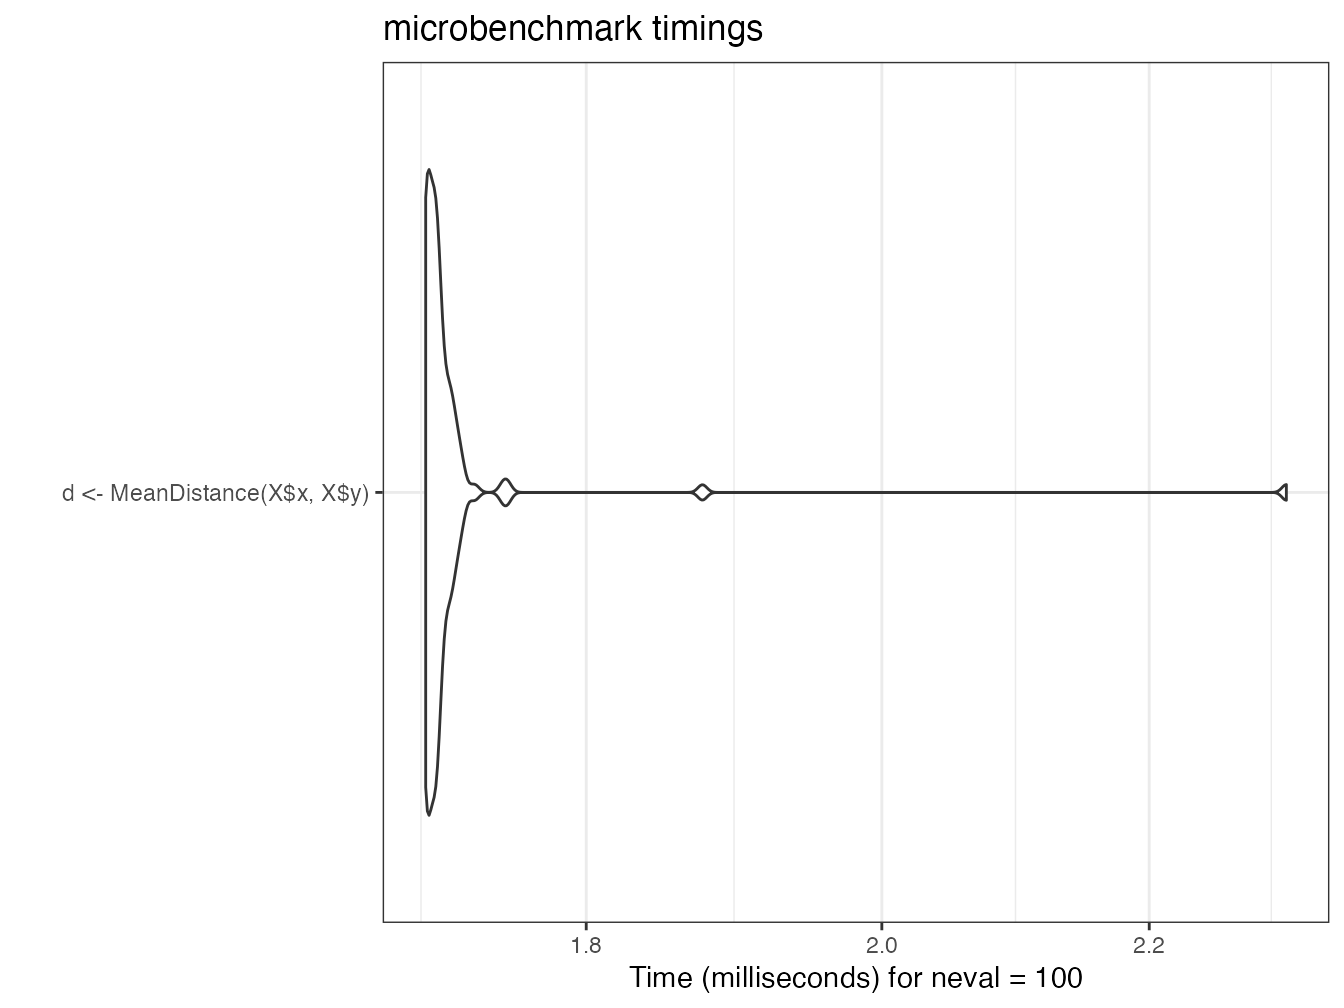
\includegraphics[width=0.8\linewidth]{WwR_files/figure-latex/RCpp-1} \end{center}

\begin{Shaded}
\begin{Highlighting}[]
\NormalTok{d}
\end{Highlighting}
\end{Shaded}

\begin{verbatim}
## [1] 0.5154879
\end{verbatim}

\normalsize

\subsection{RcppParallel}\label{rcppparallel}

\textbf{RcppParallel} allows to interface parallelized C++ code, at the cost of a more complex syntax than \textbf{RCpp}.
Documentation is available\footnote{\url{http://rcppcore.github.io/RcppParallel/}}.

The C++ function exported to R does not perform the computations but only organizes the parallel execution of another, non-exported, function of type \texttt{Worker}.

Two (C++) parallelization functions are available for two types of tasks:

\begin{itemize}
\tightlist
\item
  \texttt{parallelReduce} to accumulate a value, used here to sum distances.
\item
  \texttt{parallelFor} to fill a result matrix.
\end{itemize}

The syntax of the \texttt{Worker} is a bit tricky but simple enough to adapt: the constructors initialize the C variables from the values passed by R and declare the parallelization.

\scriptsize

\begin{Shaded}
\begin{Highlighting}[]
\CommentTok{// [[Rcpp::depends(RcppParallel)]]}
\PreprocessorTok{\#include }\ImportTok{\textless{}Rcpp.h\textgreater{}}
\PreprocessorTok{\#include }\ImportTok{\textless{}RcppParallel.h\textgreater{}}
\KeywordTok{using} \KeywordTok{namespace}\NormalTok{ Rcpp}\OperatorTok{;}
\KeywordTok{using} \KeywordTok{namespace}\NormalTok{ RcppParallel}\OperatorTok{;}

\CommentTok{// Working function, not exported}
\KeywordTok{struct}\NormalTok{ TotalDistanceWrkr }\OperatorTok{:} \KeywordTok{public}\NormalTok{ Worker}
\OperatorTok{\{}
  \CommentTok{// source vectors}
  \AttributeTok{const}\NormalTok{ RVector}\OperatorTok{\textless{}}\DataTypeTok{double}\OperatorTok{\textgreater{}}\NormalTok{ Rx}\OperatorTok{;}
  \AttributeTok{const}\NormalTok{ RVector}\OperatorTok{\textless{}}\DataTypeTok{double}\OperatorTok{\textgreater{}}\NormalTok{ Ry}\OperatorTok{;}
  
  \CommentTok{// accumulated value}
  \DataTypeTok{double}\NormalTok{ distance}\OperatorTok{;}
   
  \CommentTok{// constructors}
\NormalTok{  TotalDistanceWrkr}\OperatorTok{(}\AttributeTok{const}\NormalTok{ NumericVector x}\OperatorTok{,} \AttributeTok{const}\NormalTok{ NumericVector y}\OperatorTok{)} \OperatorTok{:}
\NormalTok{    Rx}\OperatorTok{(}\NormalTok{x}\OperatorTok{),}\NormalTok{ Ry}\OperatorTok{(}\NormalTok{y}\OperatorTok{),}\NormalTok{ distance}\OperatorTok{(}\DecValTok{0}\OperatorTok{)} \OperatorTok{\{\}}
\NormalTok{  TotalDistanceWrkr}\OperatorTok{(}\AttributeTok{const}\NormalTok{ TotalDistanceWrkr}\OperatorTok{\&}\NormalTok{ totalDistanceWrkr}\OperatorTok{,}\NormalTok{ Split}\OperatorTok{)} \OperatorTok{:}
\NormalTok{    Rx}\OperatorTok{(}\NormalTok{totalDistanceWrkr}\OperatorTok{.}\NormalTok{Rx}\OperatorTok{),}\NormalTok{ Ry}\OperatorTok{(}\NormalTok{totalDistanceWrkr}\OperatorTok{.}\NormalTok{Ry}\OperatorTok{),}\NormalTok{  distance}\OperatorTok{(}\DecValTok{0}\OperatorTok{)} \OperatorTok{\{\}}
  
  \CommentTok{// count neighbors}
  \DataTypeTok{void} \KeywordTok{operator}\OperatorTok{()(}\BuiltInTok{std::}\NormalTok{size\_t begin}\OperatorTok{,} \BuiltInTok{std::}\NormalTok{size\_t end}\OperatorTok{)} \OperatorTok{\{}
    \DataTypeTok{double}\NormalTok{ dx}\OperatorTok{,}\NormalTok{ dy}\OperatorTok{;}
    \DataTypeTok{unsigned} \DataTypeTok{int}\NormalTok{ Npoints }\OperatorTok{=}\NormalTok{ Rx}\OperatorTok{.}\NormalTok{length}\OperatorTok{();}

    \ControlFlowTok{for} \OperatorTok{(}\DataTypeTok{unsigned} \DataTypeTok{int}\NormalTok{ i }\OperatorTok{=}\NormalTok{ begin}\OperatorTok{;}\NormalTok{ i }\OperatorTok{\textless{}}\NormalTok{ end}\OperatorTok{;}\NormalTok{ i}\OperatorTok{++)} \OperatorTok{\{}
      \ControlFlowTok{for} \OperatorTok{(}\DataTypeTok{unsigned} \DataTypeTok{int}\NormalTok{ j }\OperatorTok{=}\NormalTok{ i }\OperatorTok{+} \DecValTok{1}\OperatorTok{;}\NormalTok{ j }\OperatorTok{\textless{}}\NormalTok{ Npoints}\OperatorTok{;}\NormalTok{ j}\OperatorTok{++)} \OperatorTok{\{}
          \CommentTok{// Calculate squared distance}
\NormalTok{          dx }\OperatorTok{=}\NormalTok{ Rx}\OperatorTok{[}\NormalTok{i}\OperatorTok{]} \OperatorTok{{-}}\NormalTok{ Rx}\OperatorTok{[}\NormalTok{j}\OperatorTok{];}
\NormalTok{          dy }\OperatorTok{=}\NormalTok{ Ry}\OperatorTok{[}\NormalTok{i}\OperatorTok{]} \OperatorTok{{-}}\NormalTok{ Ry}\OperatorTok{[}\NormalTok{j}\OperatorTok{];}
\NormalTok{          distance }\OperatorTok{+=}\NormalTok{ sqrt}\OperatorTok{(}\NormalTok{dx }\OperatorTok{*}\NormalTok{ dx }\OperatorTok{+}\NormalTok{ dy }\OperatorTok{*}\NormalTok{ dy}\OperatorTok{);}
      \OperatorTok{\}}
    \OperatorTok{\}}
  \OperatorTok{\}}

  \CommentTok{// join my value with that of another Sum}
  \DataTypeTok{void}\NormalTok{ join}\OperatorTok{(}\AttributeTok{const}\NormalTok{ TotalDistanceWrkr}\OperatorTok{\&}\NormalTok{ rhs}\OperatorTok{)} \OperatorTok{\{} 
\NormalTok{    distance }\OperatorTok{+=}\NormalTok{ rhs}\OperatorTok{.}\NormalTok{distance}\OperatorTok{;} 
  \OperatorTok{\}}
\OperatorTok{\};}


\CommentTok{// Exported function}
\CommentTok{// [[Rcpp::export]]}
\DataTypeTok{double}\NormalTok{ TotalDistance}\OperatorTok{(}\NormalTok{NumericVector x}\OperatorTok{,}\NormalTok{ NumericVector y}\OperatorTok{)} \OperatorTok{\{}
  
  \CommentTok{// Declare TotalDistanceWrkr instance}
\NormalTok{  TotalDistanceWrkr totalDistanceWrkr}\OperatorTok{(}\NormalTok{x}\OperatorTok{,}\NormalTok{ y}\OperatorTok{);}
  
  \CommentTok{// call parallel\_reduce to start the work}
\NormalTok{  parallelReduce}\OperatorTok{(}\DecValTok{0}\OperatorTok{,}\NormalTok{ x}\OperatorTok{.}\NormalTok{length}\OperatorTok{(),}\NormalTok{ totalDistanceWrkr}\OperatorTok{);}
  
  \CommentTok{// return the result}
  \ControlFlowTok{return}\NormalTok{ totalDistanceWrkr}\OperatorTok{.}\NormalTok{distance}\OperatorTok{;}
\OperatorTok{\}}
\end{Highlighting}
\end{Shaded}

\normalsize

The usage in R is identical to the usage of C++ functions interfaced by \textbf{RCpp}.

\scriptsize

\begin{Shaded}
\begin{Highlighting}[]
\NormalTok{(mb }\OtherTok{\textless{}{-}} \FunctionTok{microbenchmark}\NormalTok{(}
\NormalTok{  d }\OtherTok{\textless{}{-}} \FunctionTok{TotalDistance}\NormalTok{(X}\SpecialCharTok{$}\NormalTok{x, X}\SpecialCharTok{$}\NormalTok{y) }\SpecialCharTok{/}\NormalTok{ n\_points }\SpecialCharTok{/}\NormalTok{ (n\_points }\SpecialCharTok{{-}} \DecValTok{1}\NormalTok{) }\SpecialCharTok{*} \DecValTok{2}
\NormalTok{))}
\end{Highlighting}
\end{Shaded}

\begin{verbatim}
## Unit: microseconds
##                                                      expr
##  d <- TotalDistance(X$x, X$y)/n_points/(n_points - 1) * 2
##      min       lq     mean  median     uq     max neval
##  236.119 238.5995 292.4063 241.244 289.46 2364.88   100
\end{verbatim}

\begin{Shaded}
\begin{Highlighting}[]
\CommentTok{\# suppressMessages to eliminate superfluous messages}
\FunctionTok{autoplot}\NormalTok{(mb)}
\end{Highlighting}
\end{Shaded}

\begin{center}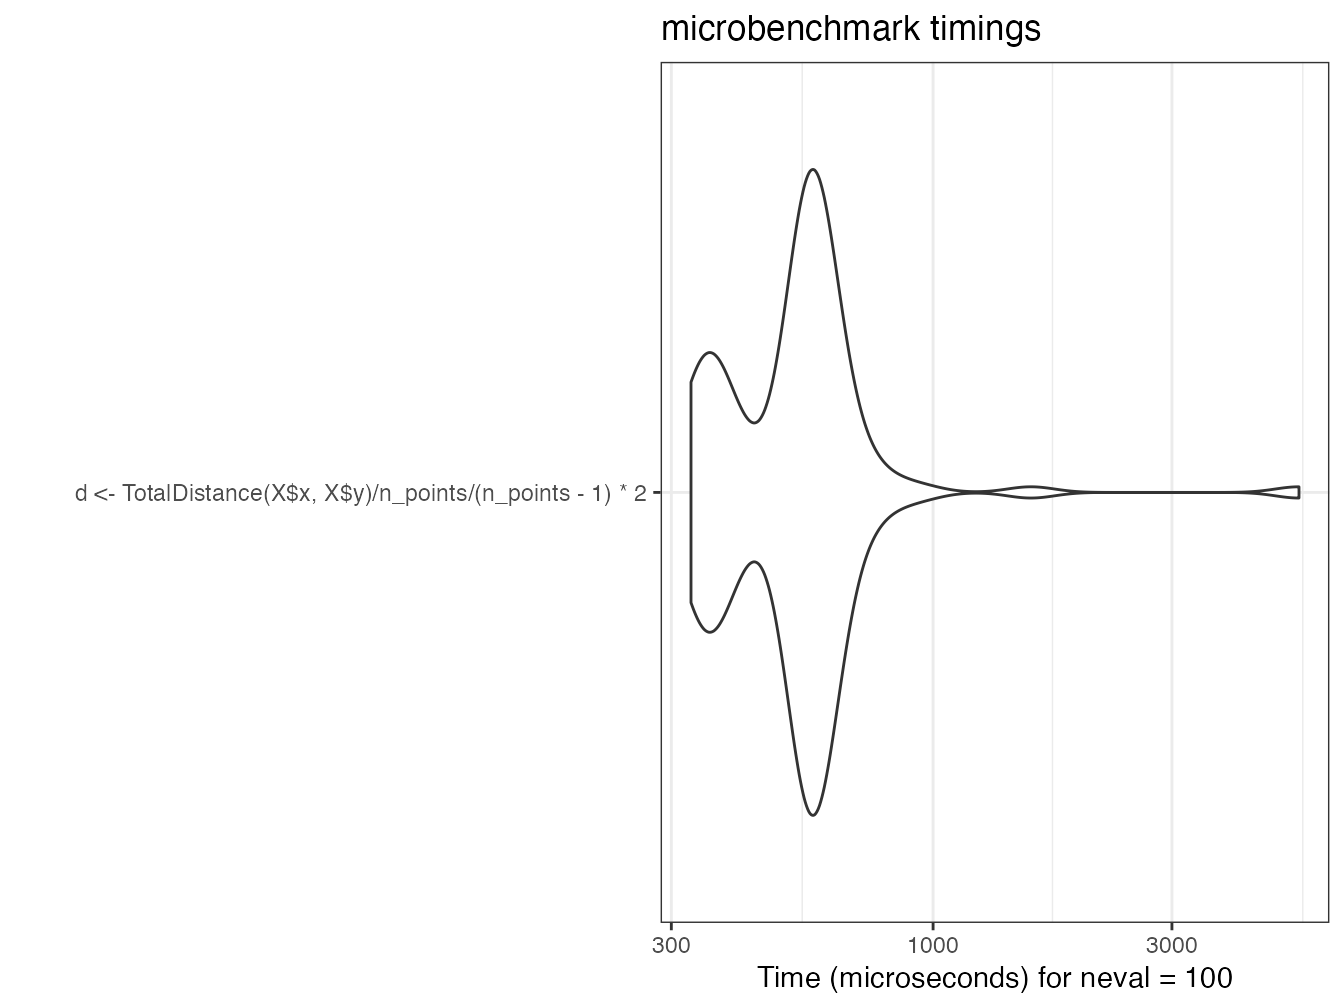
\includegraphics[width=0.8\linewidth]{WwR_files/figure-latex/RcppParallel-1} \end{center}

\begin{Shaded}
\begin{Highlighting}[]
\NormalTok{d}
\end{Highlighting}
\end{Shaded}

\begin{verbatim}
## [1] 0.5154879
\end{verbatim}

\normalsize

The setup time for parallel tasks is much longer than the serial computation time.

Multiplying the number of points by 50, the serial computation time must be multiplied by about 2500.

\scriptsize

\begin{Shaded}
\begin{Highlighting}[]
\NormalTok{n\_points }\OtherTok{\textless{}{-}} \DecValTok{50000}
\NormalTok{X }\OtherTok{\textless{}{-}} \FunctionTok{runifpoint}\NormalTok{(n\_points)}
\FunctionTok{system.time}\NormalTok{(d }\OtherTok{\textless{}{-}} \FunctionTok{MeanDistance}\NormalTok{(X}\SpecialCharTok{$}\NormalTok{x, X}\SpecialCharTok{$}\NormalTok{y))}
\end{Highlighting}
\end{Shaded}

\begin{verbatim}
##    user  system elapsed 
##   4.682   0.009   4.697
\end{verbatim}

\normalsize

In parallel, the time increases little: parallelization becomes really efficient.
This time is to be compared to that of the reference for loop, multiplied by 2500, that is \texttt{2317} seconds.

\scriptsize

\begin{Shaded}
\begin{Highlighting}[]
\FunctionTok{system.time}\NormalTok{(}
\NormalTok{  d }\OtherTok{\textless{}{-}} \FunctionTok{TotalDistance}\NormalTok{(X}\SpecialCharTok{$}\NormalTok{x, X}\SpecialCharTok{$}\NormalTok{y) }\SpecialCharTok{/}\NormalTok{ n\_points }\SpecialCharTok{/}\NormalTok{ (n\_points }\SpecialCharTok{{-}} \DecValTok{1}\NormalTok{) }\SpecialCharTok{*} \DecValTok{2}
\NormalTok{)}
\end{Highlighting}
\end{Shaded}

\begin{verbatim}
##    user  system elapsed 
##   1.432   0.021   0.603
\end{verbatim}

\normalsize

\subsection{Conclusions on code speed optimization}\label{conclusions-on-code-speed-optimization}

From this case study, several lessons can be learned:

\begin{itemize}
\tightlist
\item
  A for loop is a good basis for repetitive calculations, faster than \texttt{vapply()}, simple to read and write.
\item
  \textbf{foreach} loops are extremely effective for parallelizing for loops;
\item
  Optimized functions may exist in R packages for common tasks (here, the \texttt{pairdist()} function of \textbf{spatstat} is two orders of magnitude faster than the for loop).
\item
  The \textbf{future.apply} package makes it very easy to parallelize code that has already been written with \texttt{*apply()} functions, regardless of the hardware used;
\item
  The use of C++ code allows to speed up the calculations significantly, by three orders of magnitude here.
\item
  Parallelization of the C++ code further divides the computation time by about half the number of cores for long computations.
\end{itemize}

Beyond this example, optimizing computation time in R can be complicated if it involves parallelization and writing C++ code.
The effort must therefore be concentrated on the really long computations while the readability of the code must remain the priority for the current code.
C code is quite easy to integrate with \textbf{RCpp} and its parallelization is not very expensive with \textbf{RCppParallel}.

The use of for loops is no longer penalized since version 3.5 of R.
Writing vector code, using \texttt{sapply()} is still justified for its readability.

The choice of parallelizing the code must be evaluated according to the execution time of each parallelizable task.
If it exceeds a few seconds, parallelization is justified.

\section{Workflow}\label{sec:targets}

The \textbf{targets} package allows you to manage a \emph{workflow}, i.e.~to break down the code into elementary tasks called \emph{targets} that follow each other, the result of which is stored in a variable, itself saved on disk.
In case of a change in the code or in the data used, only the targets concerned are reevaluated.

The operation of the flow is similar to that of a cache, but does not depend on the computer on which it runs.
It is also possible to integrate the flow into a document project (see section \ref{sec:targetsmd}), and even to use a computing cluster to process the tasks in parallel.

\subsection{How it works}\label{how-it-works-1}

The documentation\footnote{\url{https://books.ropensci.org/targets/}} of \textbf{targets} is detailed and provides a worked example to learn how to use the package\footnote{\url{https://books.ropensci.org/targets/walkthrough.html}}.
It is not repeated here, but the principles of how the flow works are explained..

The workflow is unique for a given project.
It is coded in the \texttt{\_targets.R} file at the root of the project.
It contains:

\begin{itemize}
\tightlist
\item
  Global commands, such as loading packages.
\item
  A list of targets, which describe the code to be executed and the variable that stores their result.
\end{itemize}

The workflow is run by the \texttt{tar\_make()} function, which updates the targets that need it.
Its content is placed in the \texttt{\_targets} folder.
Stored variables are read by \texttt{tar\_read()}.

If the project requires long computations, \textbf{targets} can be used to run only those that are necessary.
If the project is shared or placed under source control (chapter \ref{chap-git}), the result of the computations is also integrated.
Finally, if the project is a document (chapter \ref{chap-rediger}), its formatting is completely independent of the calculation of its content, for possibly considerable time saving.

\subsection{Minimal example}\label{minimal-example}

The following example is even simpler than the one in the \textbf{targets} manual, which will allow you to go further.
It takes up the previous case study: a set of points is generated and the average distance between the points is calculated.
A map of the points is also drawn.
Each of these three operations is a target in the vocabulary of \textbf{targets}.

The workflow file is therefore the following:

\scriptsize

\begin{Shaded}
\begin{Highlighting}[]
\CommentTok{\# File \_targets.R }
\FunctionTok{library}\NormalTok{(}\StringTok{"targets"}\NormalTok{)}
\FunctionTok{tar\_option\_set}\NormalTok{(}\AttributeTok{packages =} \FunctionTok{c}\NormalTok{(}\StringTok{"spatstat"}\NormalTok{, }\StringTok{"dbmss"}\NormalTok{))}
\FunctionTok{list}\NormalTok{(}
  \CommentTok{\# Draw points}
  \FunctionTok{tar\_target}\NormalTok{(X,}
    \FunctionTok{runifpoint}\NormalTok{(n\_points)}
\NormalTok{  ),}
  \CommentTok{\# Choose Parameters}
  \FunctionTok{tar\_target}\NormalTok{(n\_points,}
    \DecValTok{1000}
\NormalTok{  ),}
  \CommentTok{\# Average Distance}
  \FunctionTok{tar\_target}\NormalTok{(d,}
    \FunctionTok{sum}\NormalTok{(}\FunctionTok{pairdist}\NormalTok{(X)) }\SpecialCharTok{/}\NormalTok{ n\_points }\SpecialCharTok{/}\NormalTok{ (n\_points }\SpecialCharTok{{-}} \DecValTok{1}\NormalTok{)}
\NormalTok{  ),}
  \CommentTok{\# Map}
  \FunctionTok{tar\_target}\NormalTok{(map, }
    \FunctionTok{autoplot}\NormalTok{(}\FunctionTok{as.wmppp}\NormalTok{(X))}
\NormalTok{  )}
\NormalTok{)}
\end{Highlighting}
\end{Shaded}

\normalsize

The global commands consist in loading the \textbf{targets} package itself and then listing the packages needed for the code.
The execution of the workflow takes place in a new instance of R.

The targets are then listed.
Each one is declared by the \texttt{tar\_target()} function whose first argument is the name of the target, which will be the name of the variable that will receive the result.
The second argument is the code that produces the result.
Targets are very simple here and can be written in a single command.
When this is not the case, each target can be written as a function, stored in a separate code file loaded by the \texttt{source()} function at the beginning of the workflow file.

The \texttt{tar\_visnetwork} command displays the sequence of targets and their possibly obsolete status.

\scriptsize

\begin{Shaded}
\begin{Highlighting}[]
\FunctionTok{library}\NormalTok{(}\StringTok{"targets"}\NormalTok{)}
\FunctionTok{tar\_visnetwork}\NormalTok{()}
\end{Highlighting}
\end{Shaded}

\normalsize

The order of declaration of the targets in the list is not important: they are ordered automatically.

The workflow is run by \texttt{tar\_make()}.

\scriptsize

\begin{Shaded}
\begin{Highlighting}[]
\FunctionTok{tar\_make}\NormalTok{()}
\end{Highlighting}
\end{Shaded}

\begin{verbatim}
## ▶ dispatched target n_points
## ● completed target n_points [0.83 seconds, 53 bytes]
## ▶ dispatched target X
## ● completed target X [0.002 seconds, 11.059 kilobytes]
## ▶ dispatched target d
## ● completed target d [0.011 seconds, 55 bytes]
## ▶ dispatched target map
## ● completed target map [0.033 seconds, 187.39 kilobytes]
## ▶ ended pipeline [0.991 seconds]
\end{verbatim}

\normalsize

The workflow is now up to date and \texttt{tar\_make()} does not recompute anything.

\scriptsize

\begin{Shaded}
\begin{Highlighting}[]
\FunctionTok{tar\_visnetwork}\NormalTok{()}
\end{Highlighting}
\end{Shaded}

\begin{Shaded}
\begin{Highlighting}[]
\FunctionTok{tar\_make}\NormalTok{()}
\end{Highlighting}
\end{Shaded}

\begin{verbatim}
## ✔ skipping targets (1 so far)...
## ✔ skipped pipeline [0.037 seconds]
\end{verbatim}

\normalsize

The results are read by \texttt{tar\_read()}.

\scriptsize

\begin{Shaded}
\begin{Highlighting}[]
\FunctionTok{tar\_read}\NormalTok{(d)}
\end{Highlighting}
\end{Shaded}

\begin{verbatim}
## [1] 0.5165293
\end{verbatim}

\begin{Shaded}
\begin{Highlighting}[]
\FunctionTok{tar\_read}\NormalTok{(map)}
\end{Highlighting}
\end{Shaded}

\begin{center}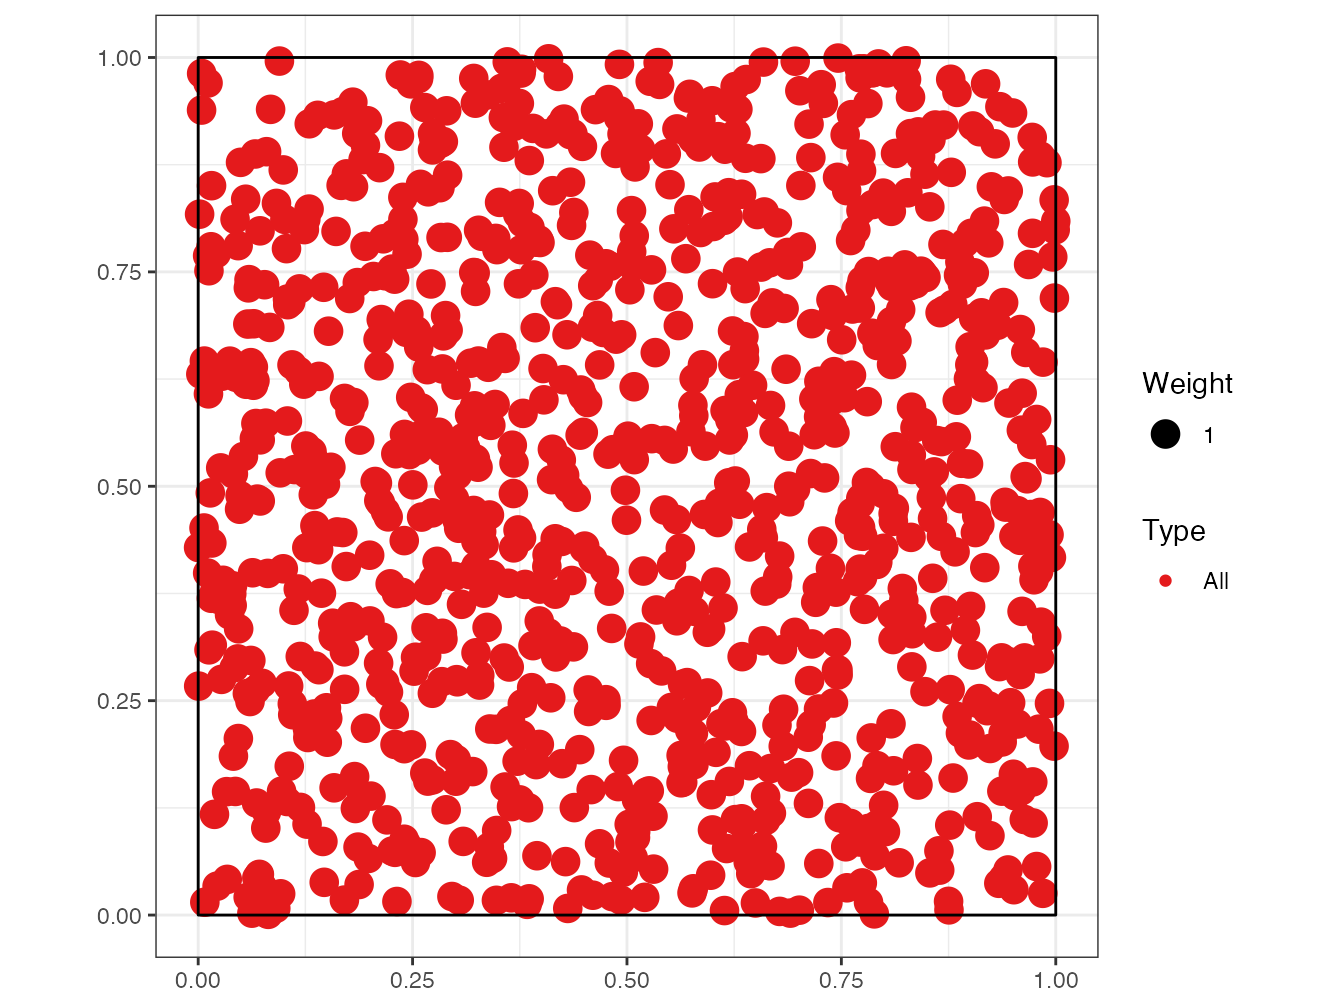
\includegraphics[width=0.8\linewidth]{WwR_files/figure-latex/tar_read-1} \end{center}

\normalsize

\subsection{Practical interest}\label{practical-interest}

In this example, \textbf{targets} complicates writing the code and \texttt{tar\_make()} is much slower than simply executing the code it processes because it has to check if the targets are up to date.
In a real project that requires long computations, processing the status of the targets is negligible and the time saved by just evaluating the necessary targets is considerable.
The definition of targets remains a constraint, but forces the user to structure their project rigorously.

\chapter{Git and GitHub}\label{chap-git}

\toc{1}

Source control consists in recording all the modifications made on the tracked files.
The advantages are numerous: traceability and security of the project, possibility to collaborate efficiently, to go back, to try new developments without jeopardizing the stable version\ldots{}

\section{Principles}\label{sec:principes-git}

\subsection{Source control}\label{sec:git-cds}

The standard tool today is \emph{git}.

The git commands can be executed in the RStudio terminal.



\scriptsize

\begin{figure}

{\centering 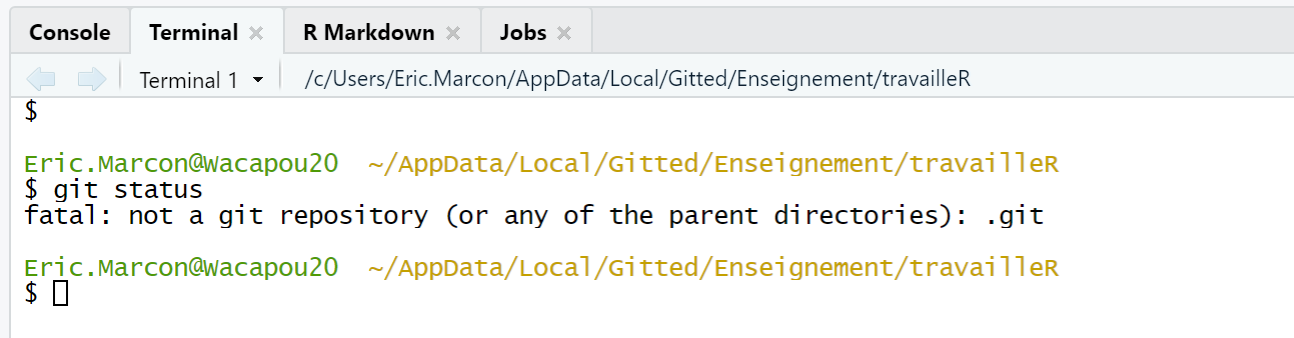
\includegraphics[width=0.8\linewidth]{images/git-Status} 

}

\caption{Screenshot of the RStudio terminal. The \texttt{git\ status} command, which is supposed to describe the state of the repository, returns an error if the R project is not under source control.}\label{fig:git-Status}
\end{figure}

\normalsize

The \texttt{git\ status} command (figure \ref{fig:git-Status}) returns the status of the repository, that is, the set of data managed by git to track the current project.

RStudio integrates a graphical interface for git that is sufficient to do without the command line for standard use, presented here.

\subsection{git and GitHub}\label{git-and-github-1}

\emph{git} is the software installed on the workstation.

\emph{GitHub} is a web platform\footnote{\url{https://github.com/}}, which allows to share the content of git repositories (to work with several people) and to share documentation in the form of a web site (\emph{GitHub Pages}).

As GitHub allows at least the backup of git repositories, the two are always used together.
GitHub is not the only platform that can be used but the main one.
Alternatives are Bitbucket\footnote{\url{https://bitbucket.org/}} and GitLab\footnote{\url{https://about.gitlab.com/}} for example.

\section{Create a new repository}\label{sec:creerdepot}

\subsection{From an existing project}\label{from-an-existing-project}

In an existing R project, enable source control in the project options (figure \ref{fig:git-Project}).
The command executed is \texttt{git\ init}.
Restart RStudio on demand.



\scriptsize

\begin{figure}

{\centering 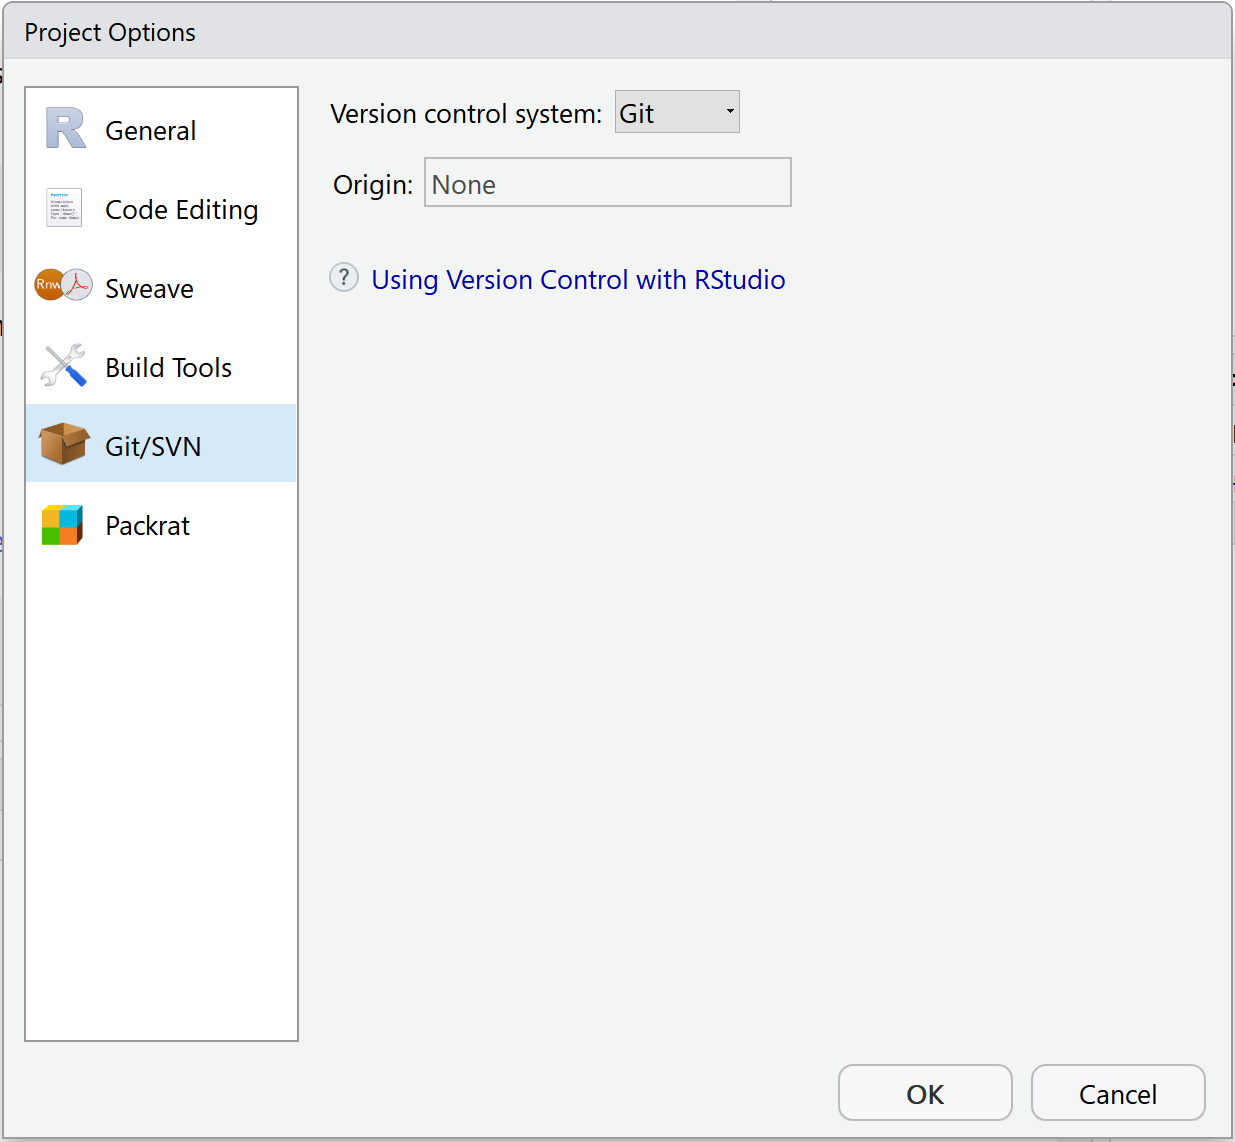
\includegraphics[width=0.8\linewidth]{images/git-Project} 

}

\caption{Activation of source control in the menu \enquote{Tools \textgreater{} Project Options\ldots{}}.}\label{fig:git-Project}
\end{figure}

\normalsize

A new \emph{Git} window appears in the upper right panel.
It contains the list of project files (figure \ref{fig:git-Fichiers}).



\scriptsize

\begin{figure}

{\centering 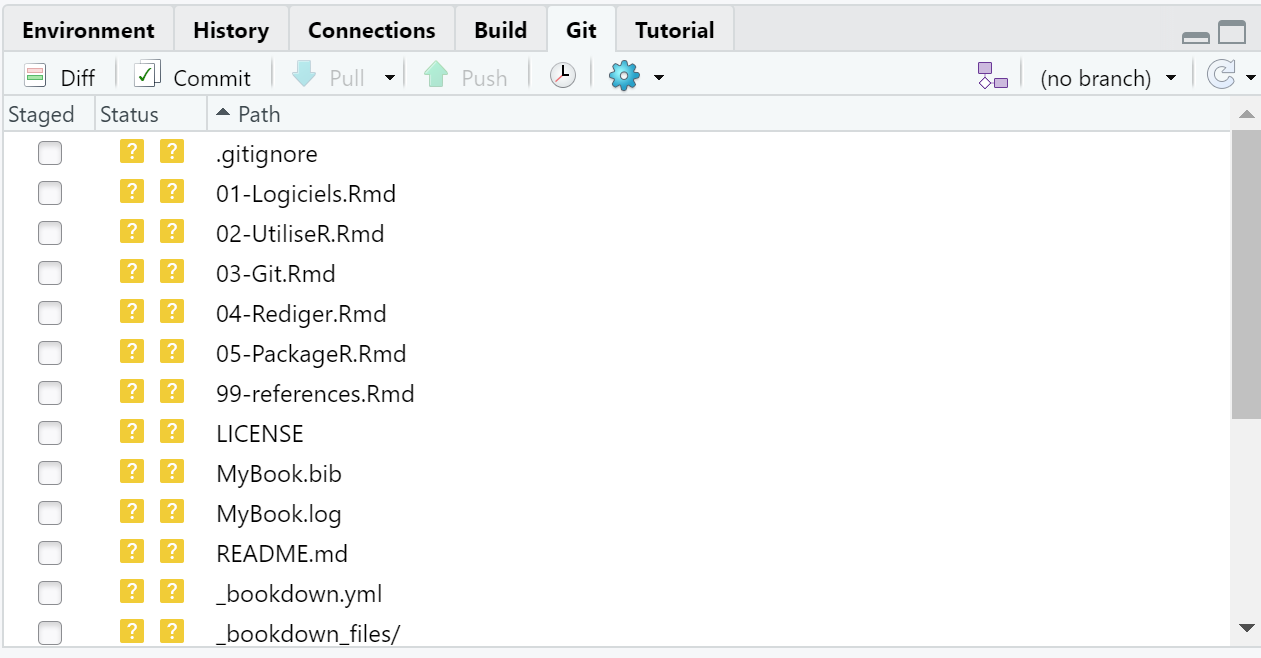
\includegraphics[width=0.8\linewidth]{images/git-Fichiers} 

}

\caption{Project files, not yet taken into account by git.}\label{fig:git-Fichiers}
\end{figure}

\normalsize

At this point, the files are not taken into account by git: their status is a double yellow question mark.
For git, the local working directory is a \emph{sandbox} where all changes are possible without consequences.

The \texttt{.gitignore} file contains the list of files that are never intended to be taken into account, so there is no need to display them in the list: automatically produced intermediate files for example.
The syntax of \texttt{.gitignore} files is detailed in the git\footnote{\url{https://git-scm.com/docs/gitignore}} documentation.
As a general rule, use an existing file: document templates in particular include their \texttt{.gitignore} file.

\subsection{Taking files into account}\label{taking-files-into-account}

In the git window, checking the \emph{Staged} checkbox allows you to stage each file.
The command executed is \texttt{git\ add\ \textless{}FileName\textgreater{}}.
Files taken into account the first time have the status \enquote{A} for \enquote{Added}.

The files taken into account are part of the git \emph{index}.

\subsection{Committing changes}\label{committing-changes}



\scriptsize

\begin{figure}

{\centering 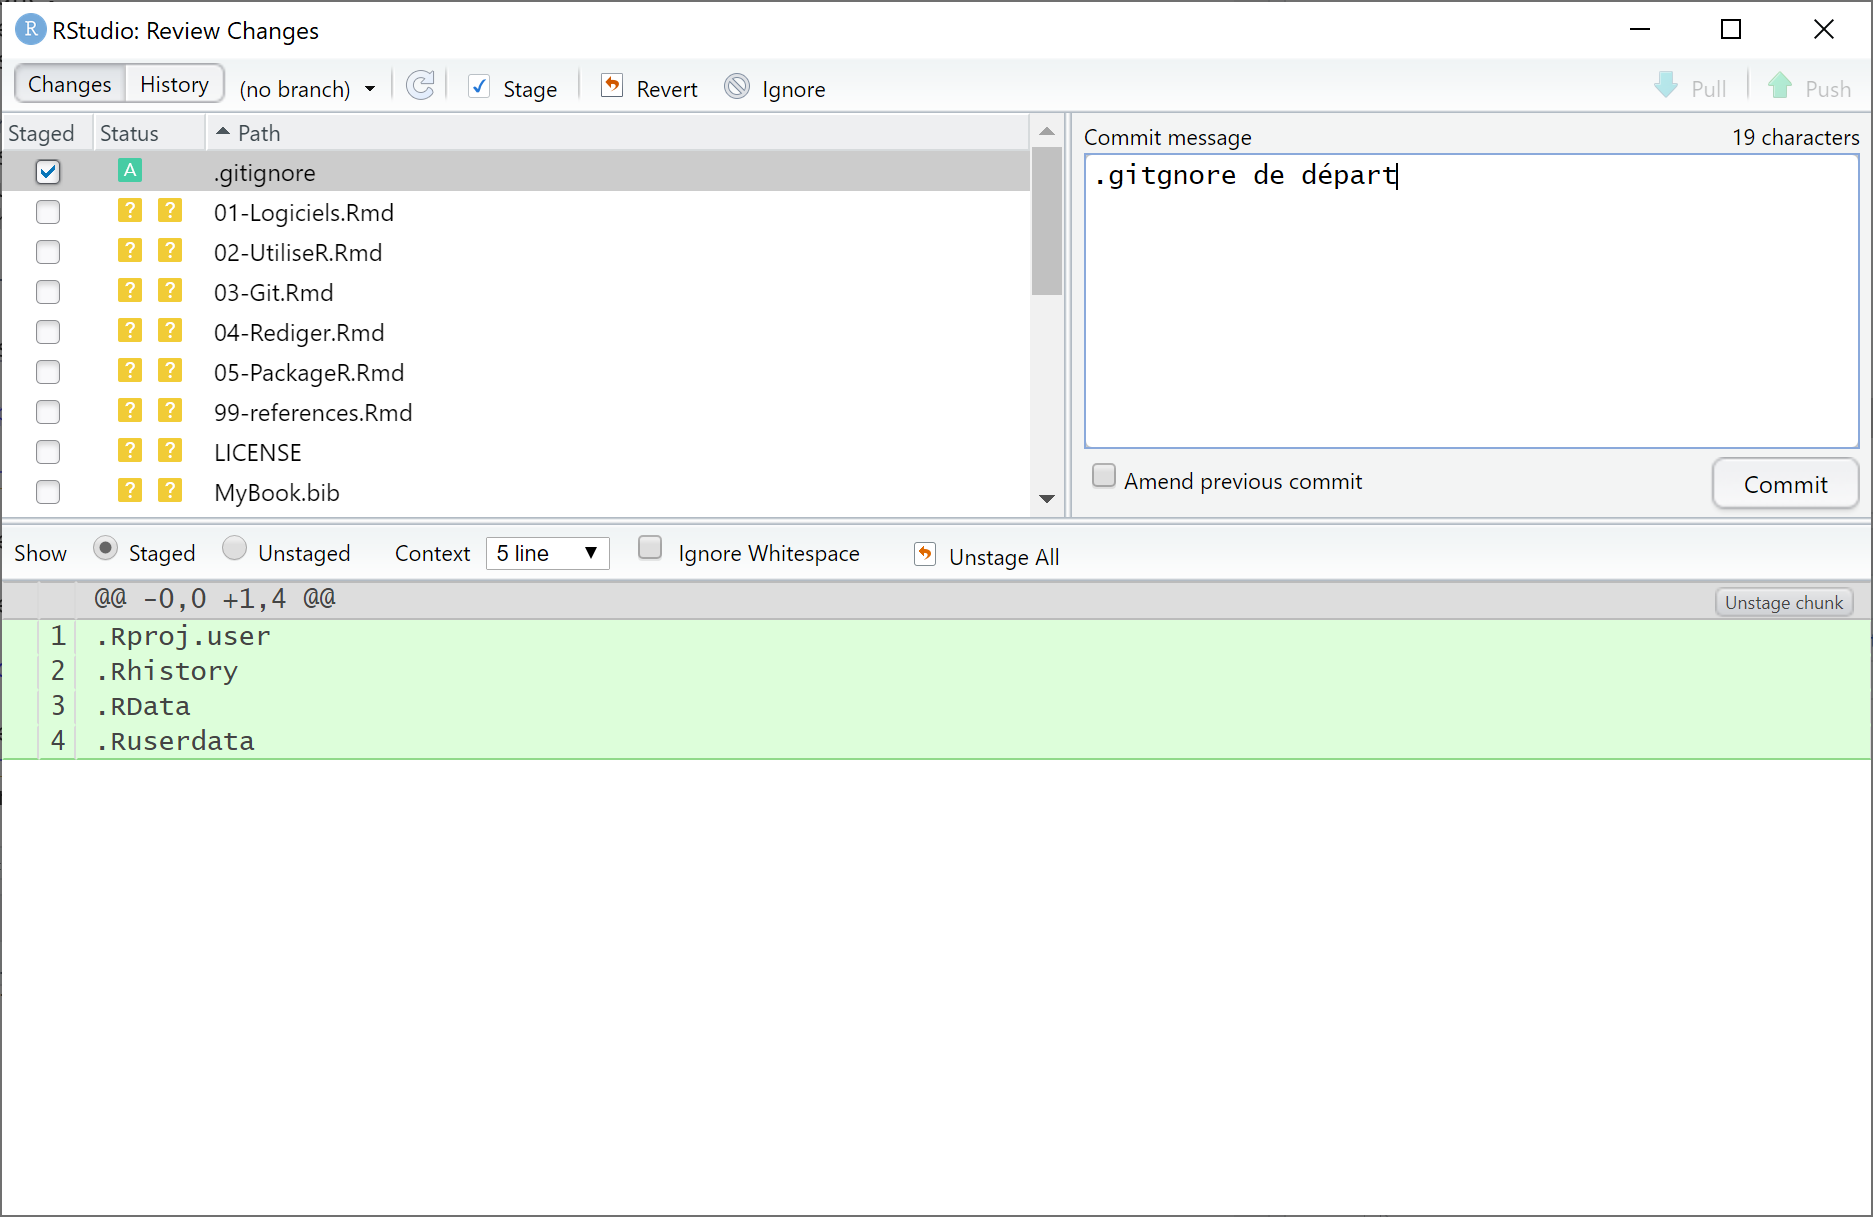
\includegraphics[width=0.8\linewidth]{images/git-Commit} 

}

\caption{Commit window.}\label{fig:git-Commit}
\end{figure}

\normalsize

The staged files can be validated (\emph{Committed}) by clicking on the \enquote{Commit} button in the \emph{Git} window.
A new window opens (figure \ref{fig:git-Commit}), which allows to visualize all the modifications by file (additions in green, deletions in red).
The modification grain treated by git is the text line, ended by a line break.
Binary files such as images are processed as a whole.

Each commit comes with a description text.
The first line is the short description.
A detailed description can be added after a line break.
For the readability of the project history, each commit corresponds to an action, corresponding to the short description: not all modified files are necessarily taken into account and validated at once.
The command executed is \texttt{git\ commit\ -m\ "Commit\ message"}.



\scriptsize

\begin{figure}

{\centering 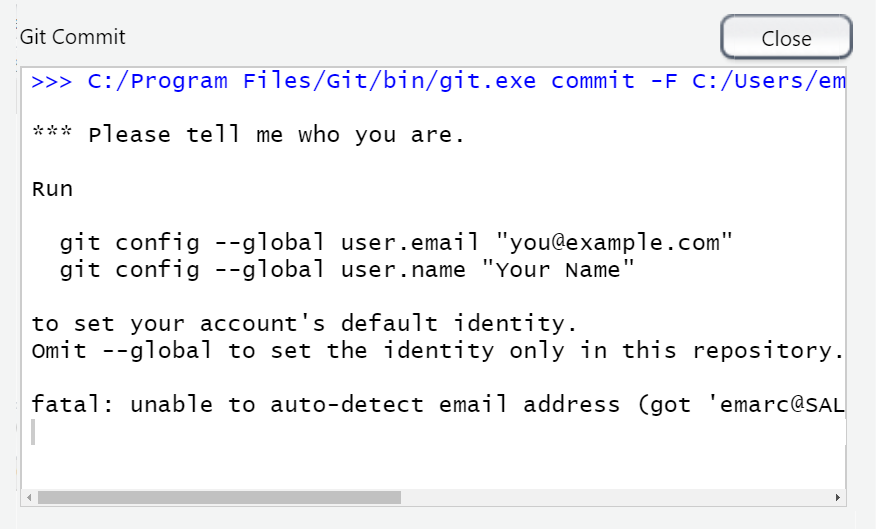
\includegraphics[width=0.8\linewidth]{images/git-id} 

}

\caption{Identification window.}\label{fig:git-id}
\end{figure}

\normalsize

Commits are linked to their author, who must be identified by git.
Generally, git uses the system information.
If it does not succeed, a window asks the user to identify himself before making his first \emph{commit} (figure \ref{fig:git-id}).
The commands shown are to be executed in the RStudio terminal.
They can also be used to check the values known by git:

\begin{verbatim}
git config user.name
git config user.email
\end{verbatim}

After the first commit, the main branch of the repository, called \enquote{master}, is created.
A branch is a version of the repository, with its own history and therefore its own files.
Branches allow:

\begin{itemize}
\tightlist
\item
  To develop new features in a project, without disturbing the main branch which may contain a stable version.
  If the development is accepted, its branch can be merged with the \emph{master} branch to create a new stable version.
\item
  To host files totally different from those of the main branch, for other purposes.
  On GitHub, a project's web pages can be placed in a branch called \enquote{gh-pages} which will never be merged.
\end{itemize}

The git repository is fully constituted.
In git vocabulary, it consists of three \emph{trees} (figure \ref{fig:git-Trees}):

\begin{itemize}
\tightlist
\item
  The working directory, or sandbox, which contains files that are not staged: unknown, modified, deleted or renamed (\enquote{Staged} box unchecked).
\item
  The index, which contains the files taken into account (\enquote{Staged} box checked).
\item
  The head, which contains the validated files.
\end{itemize}



\scriptsize

\begin{figure}

{\centering 
\includegraphics[width=0.8\linewidth]{images/git-Trees} 

}

\caption{git's trees. Source: \url{https://rogerdudler.github.io/git-guide/index.fr.html}}\label{fig:git-Trees}
\end{figure}

\normalsize

The status of the files is represented by two icons in the RStudio \emph{Git} window: two question marks when they are not in git's index.
Then, the icon on the right describes the difference between the working directory and the index.
The one on the left describes the difference between the index and the head.
So a modified file will have the \texttt{M} icon displayed on the right before it is taken into account, then on the left after it is taken into account.
It is possible, although better to avoid it, to modify again a file that has been taken into account before it is validated: then, both icons will be displayed.

\subsection{Create an empty repository on GitHub}\label{create-an-empty-repository-on-github}



\scriptsize

\begin{figure}

{\centering 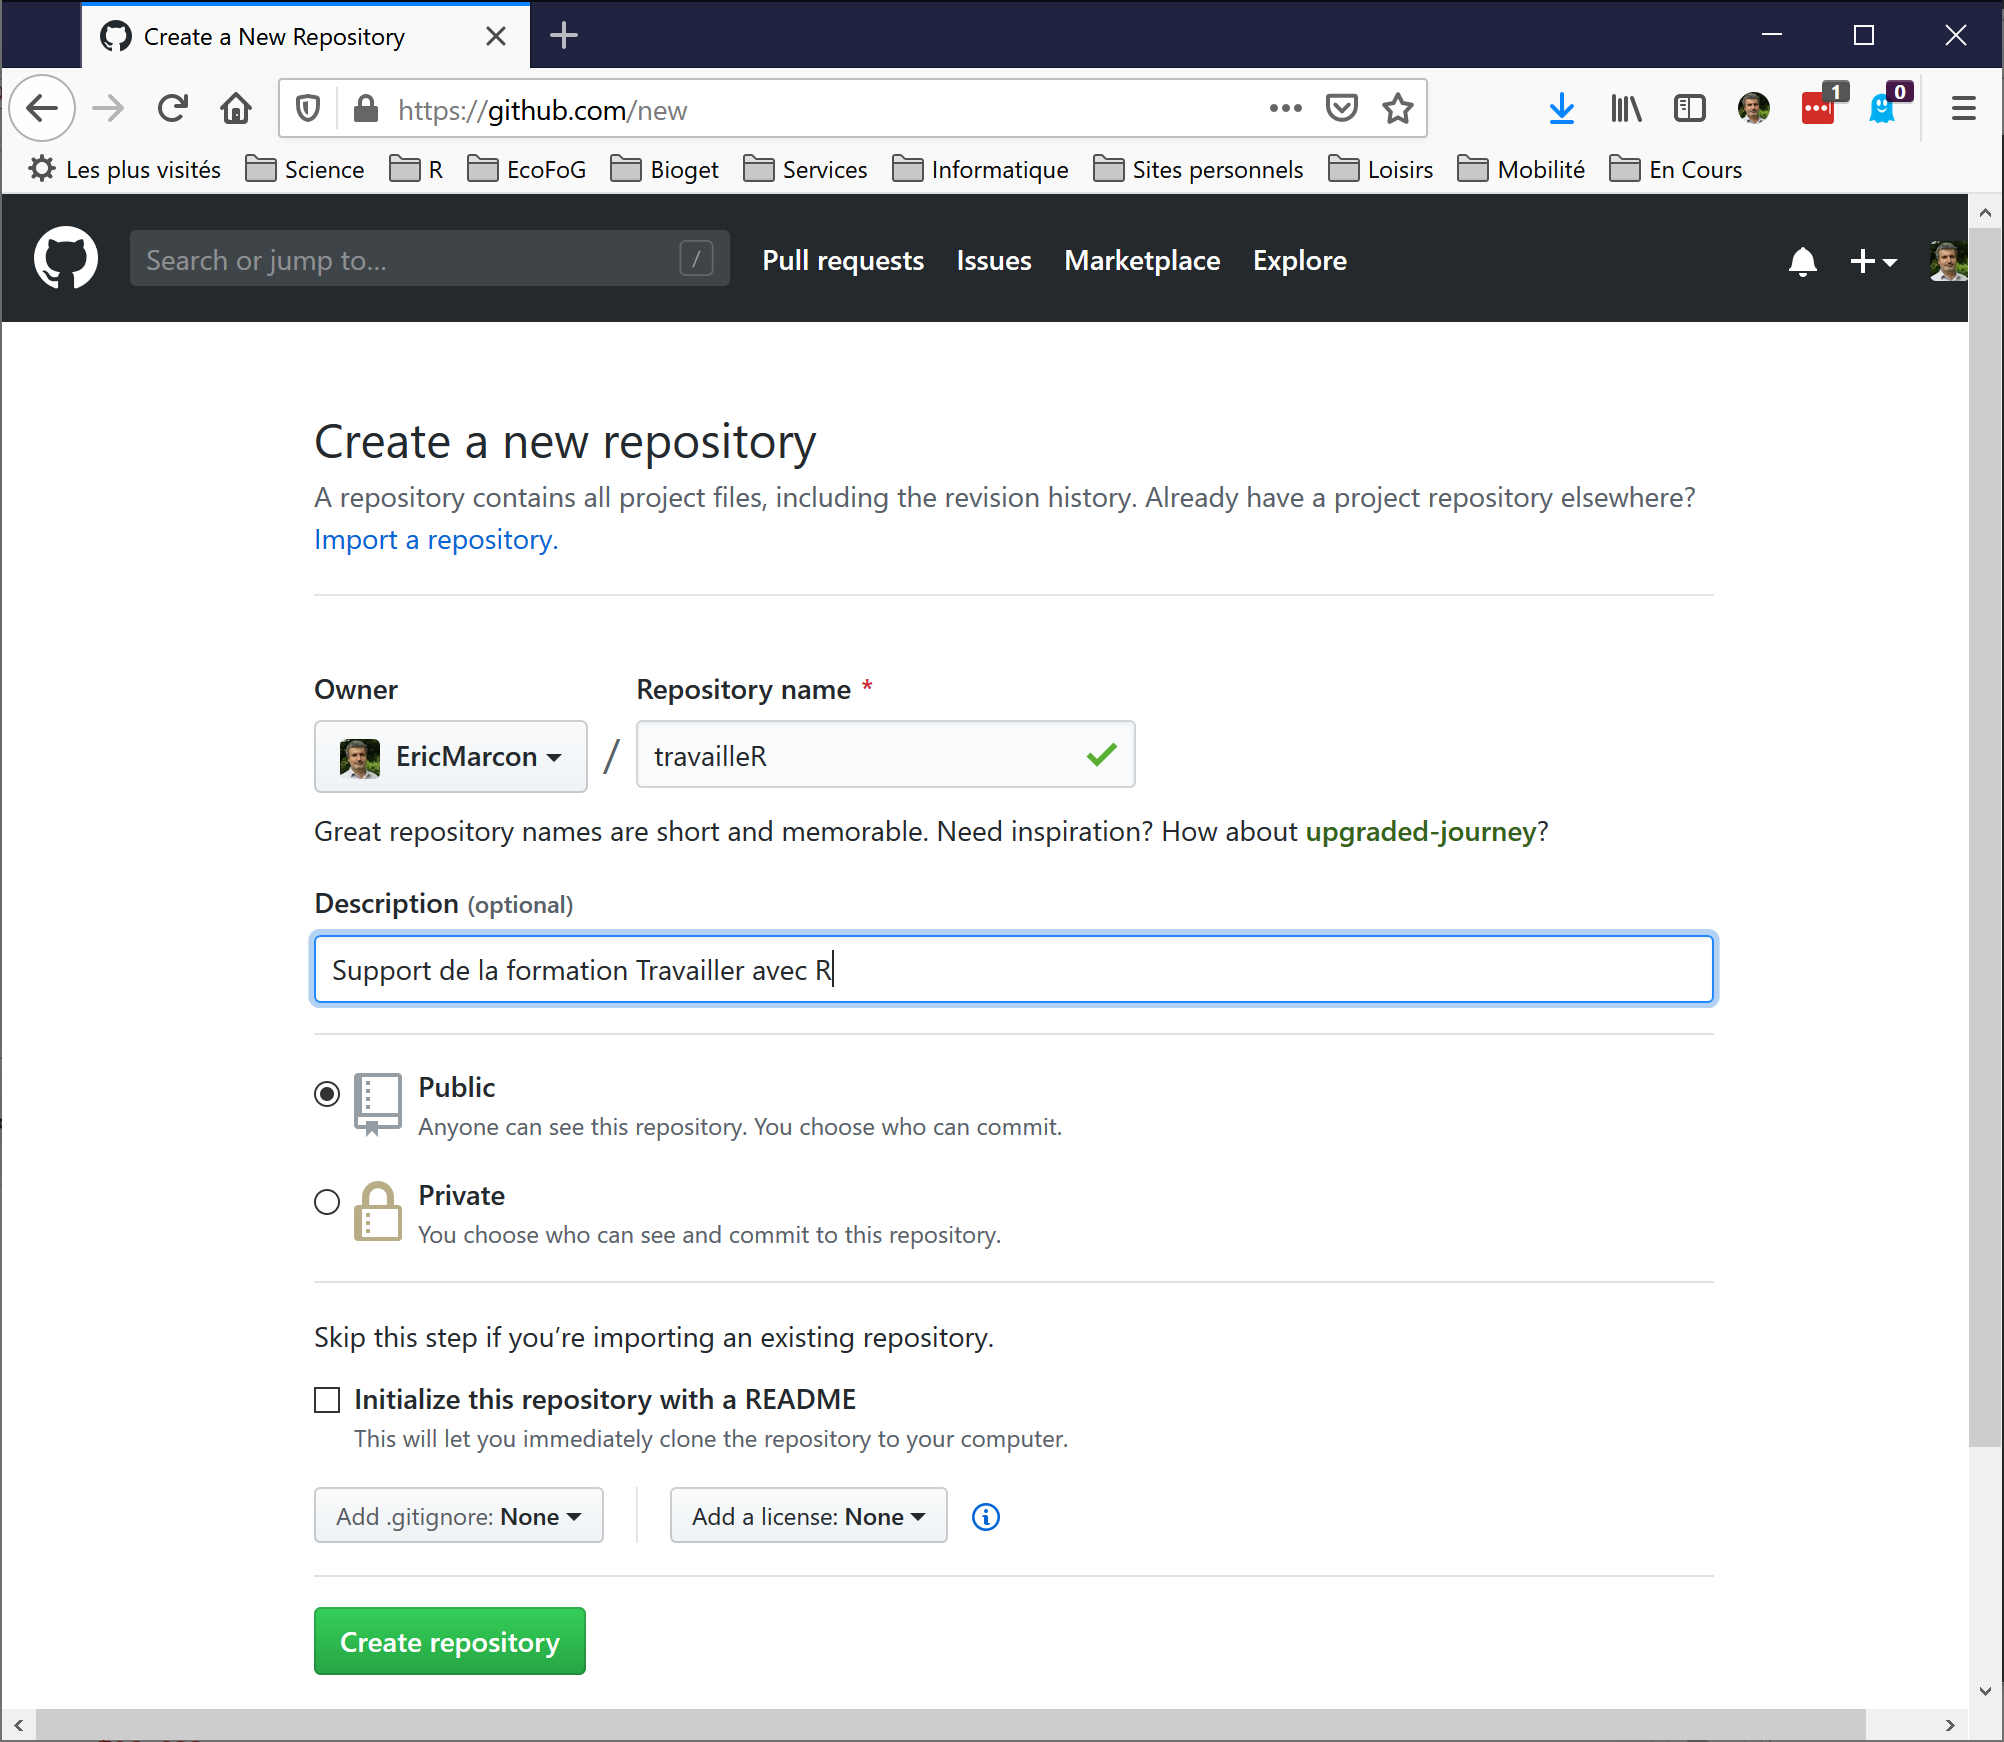
\includegraphics[width=0.8\linewidth]{images/CreateRepo} 

}

\caption{Create a repository on GitHub.}\label{fig:CreateRepo}
\end{figure}

\normalsize

An empty repository on GitHub must be created (figure \ref{fig:CreateRepo}):

\begin{itemize}
\tightlist
\item
  On GitHub, click on the green \enquote{New repository} button.
\item
  Enter the name of the repository, identical to the local R project.
\item
  Add a description, which will appear only on the GitHub page of the repository.
\item
  Choose the status of the repository:

  \begin{itemize}
  \tightlist
  \item
    Public: visible to everyone.
  \item
    Private: visible only to project collaborators, which excludes adding web pages.
  \end{itemize}
\item
  Do not add any \texttt{README}, \texttt{.gitignore} or license: the project must be empty.
\item
  Click on \enquote{create Repository}.
\item
  Copy the address of the repository (\url{https://github.com/}\ldots{} or \href{mailto:git@github.com}{\nolinkurl{git@github.com}}:\ldots).
\end{itemize}

The choice of the address is linked to the authentication method.
SSH authentication (see section \ref{sec:SSH}) is preferred.

\subsection{Linking git and GitHub}\label{linking-git-and-github}

In RStudio, a first \emph{commit} must at least have taken place for the main branch of the project, named \enquote{master}, to exist.
At the top right of the \emph{Git} window (figure \ref{fig:git-Fichiers}), it shows \enquote{(no branch)} before that.
Then it is displayed \enquote{master}, the default name of the main branch of the project.
The project can then be linked to the GitHub repository.

\subsubsection{Graphical method}\label{graphical-method}

Click on the purple button next to \enquote{master}: a window appears (usually used for creating a new branch, see section \ref{sec:branches}).
Enter the name of the \enquote{master} branch, click on \enquote{Add Remotes} and complete:

\begin{itemize}
\tightlist
\item
  Remote Name: \texttt{origin}.
\item
  Remote URL: paste the address of the GitHub repository.
\item
  Click on \enquote{Add}.
\end{itemize}

Check the \enquote{Sync with Remote} box.

At the message indicating that a \emph{master} branch already exists, click on \enquote{Overwrite}.

\subsubsection{On the command line}\label{on-the-command-line}

Instead of the previous manipulation, the link between Git and GitHub can be set up by some git commands executed in the RStudio terminal.
These are displayed on the home page of any newly created empty repository on GitHub and can therefore be copied and pasted directly to the terminal.

\begin{verbatim}
git remote add origin git@github.com:<GitHubID>/<RepoID>.git
git branch -M master
git push -u origin master
\end{verbatim}

The first command declares the GitHub repository as a remote repository.
The name \emph{origin} is a git convention.
It can be changed, but the organization of the project will be more readable if it follows the convention.
The repository address is \texttt{https://github.com/\textless{}GitHubID\textgreater{}/\textless{}RepoID\textgreater{}.git} if HTTPS authentication is chosen.

The following commands activate the main branch of the project and push its content to GitHub.

Be careful with the name of the main branch (see section \ref{sec:branches}): by default, it is called \enquote{master} in a project created in RStudio but \enquote{main} on GitHub.
The above command lines provided by GitHub therefore replace \texttt{master} with \texttt{main} and must be corrected to match the name of the branch created by RStudio.

\subsubsection{Authentication}\label{authentication}

If HTTPS authentication is chosen, the first time RStudio connects to GitHub, a window allows you to enter your GitHub credentials (figure \ref{fig:git-PAT}).



\scriptsize

\begin{figure}

{\centering 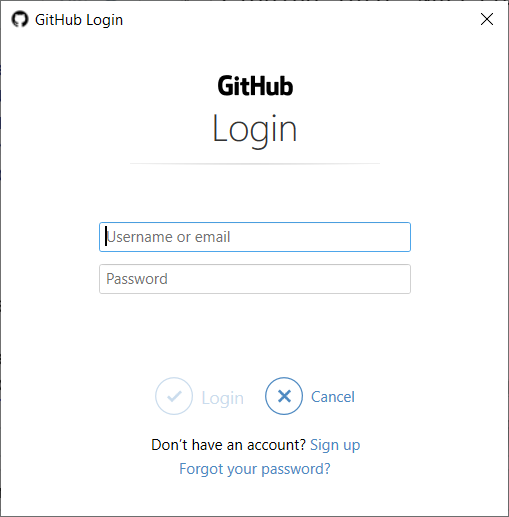
\includegraphics[width=0.8\linewidth]{images/git-PAT} 

}

\caption{Identification HTTPS sur GitHub.}\label{fig:git-PAT}
\end{figure}

\normalsize

As of August 2021, GitHub no longer accepts the user's account password for this authentication: the personal token (PAT) created in section \ref{sec:pat} must be entered instead.

If SSH authentication is chosen and has been configured at git installation (section \ref{sec:SSH}), no action is necessary.

\subsection{Push the first modifications}\label{push-the-first-modifications}

The previous manipulation has automatically pushed the validated modifications on GitHub.
Afterwards, you will have to click on the \enquote{Push} button of the \emph{Git} window to do it.

On GitHub, the files resulting from the modifications recorded by git are now visible.

Each commit done locally is counted by git and a message \enquote{Your branch is ahead of \enquote*{origin/master} by \emph{n} commits} displayed in the top of the \emph{Git} window indicates that it is time to update GitHub by pushing all these commits.
Click on the \enquote{Push} button to do so.

At this point, the project should have a \texttt{README.md} file that presents its contents on GitHub.
Its minimal content is a title and a few lines of description:

\begin{verbatim}
# Project name

Description in a few lines.
\end{verbatim}

It is advisable to use badges\footnote{\url{https://github.com/orangemug/stability-badges}}, to be placed just after the title, to declare the maturity status of the project, for example:

\begin{verbatim}
![stability-wip](https://img.shields.io/badge/|>
stability-work_in_progress-lightgrey.svg)
\end{verbatim}

\subsection{Clone a repository from GitHub}\label{clone-a-repository-from-github}



\scriptsize

\begin{figure}

{\centering 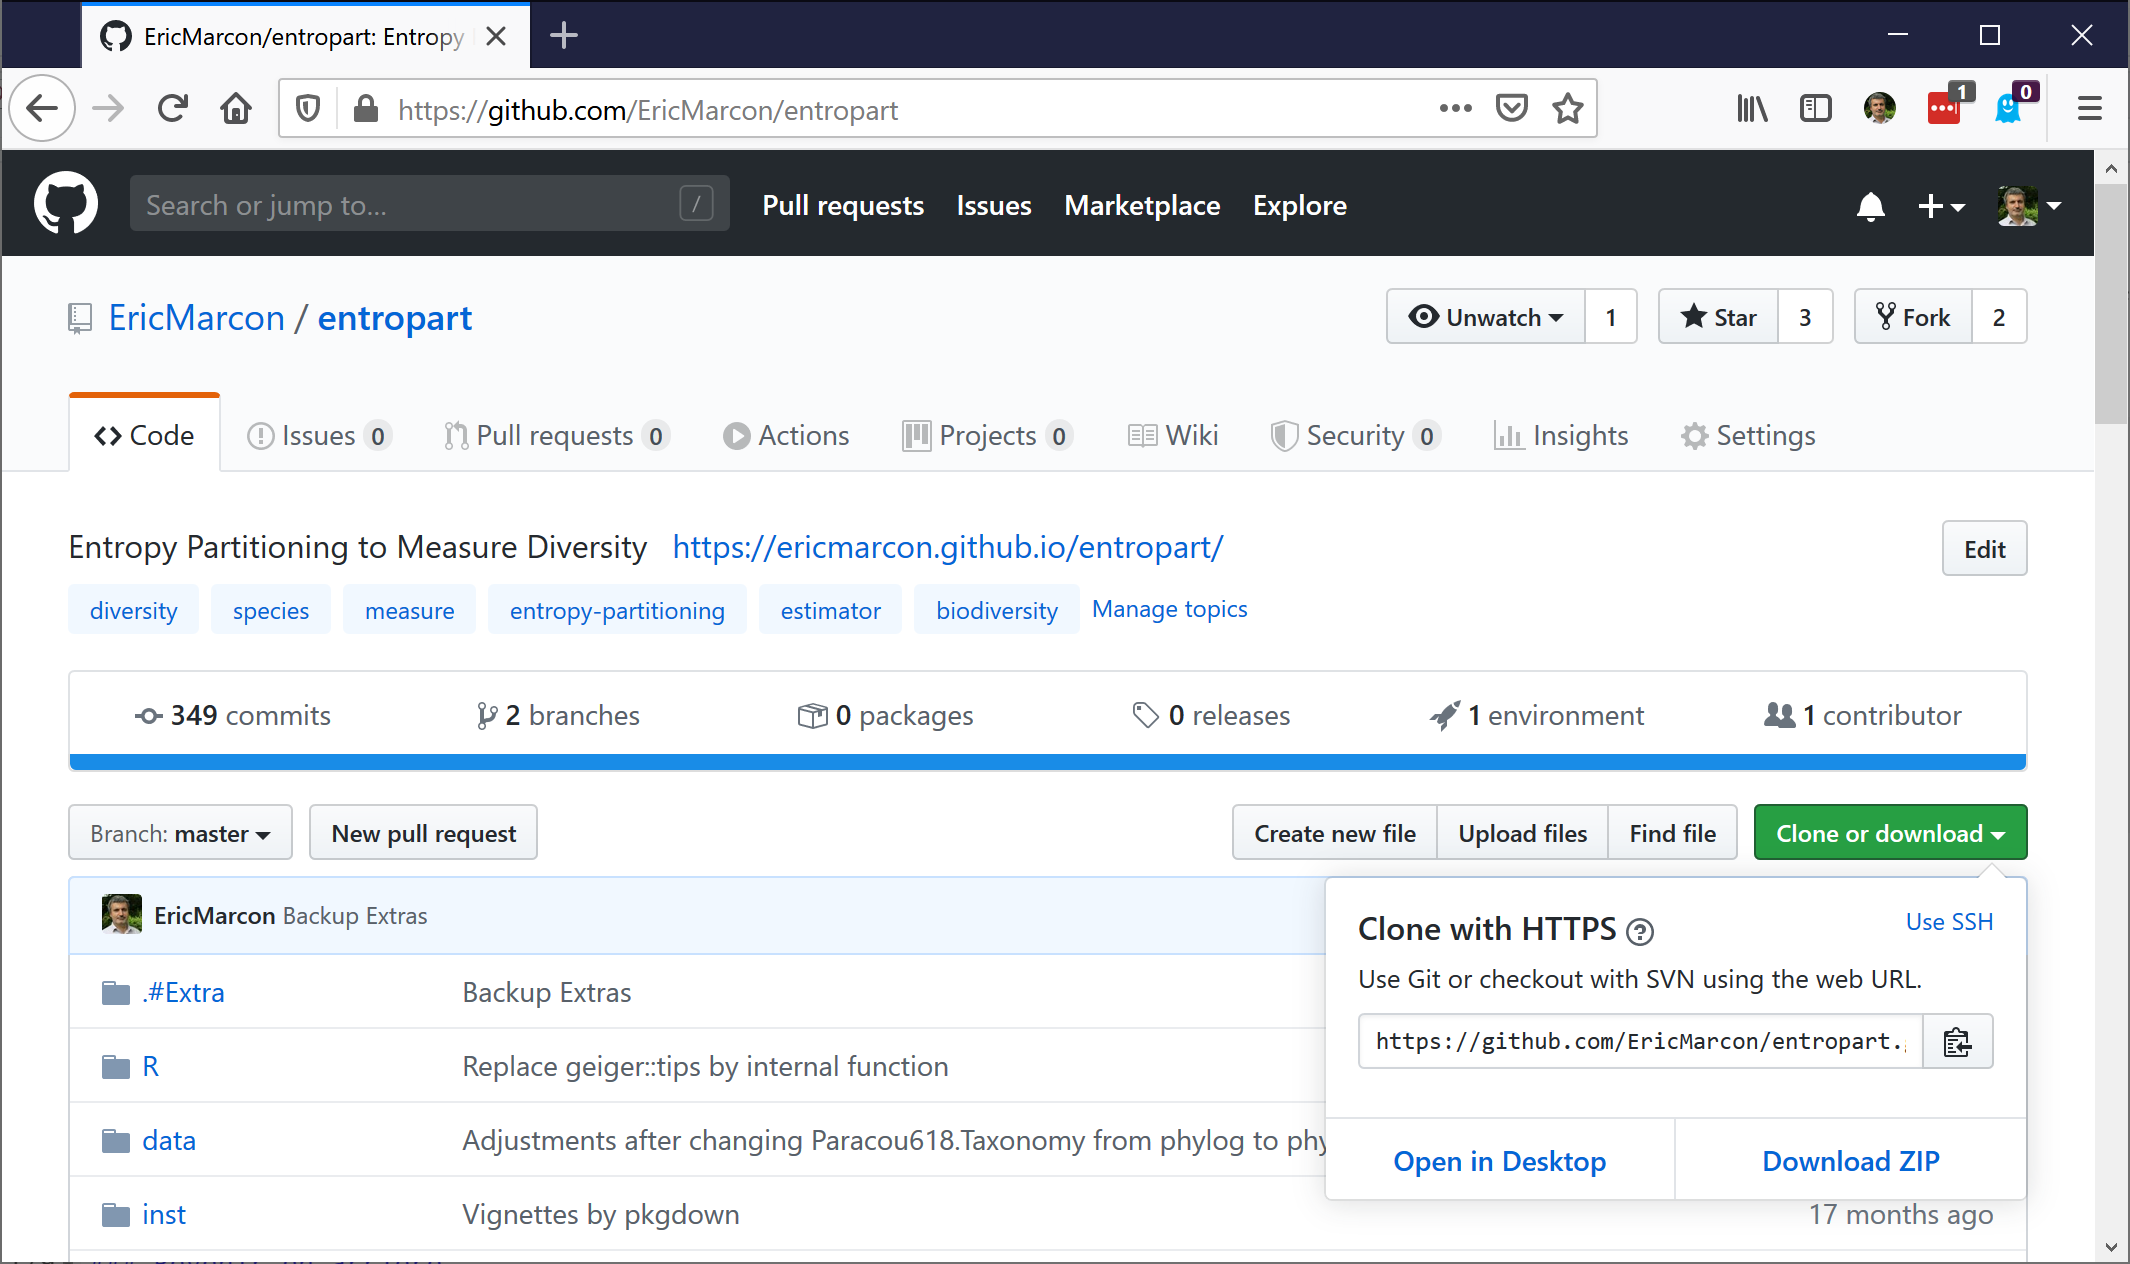
\includegraphics[width=0.8\linewidth]{images/git-Clone} 

}

\caption{Cloning a repository from \emph{GitHub.}}\label{fig:git-Clone}
\end{figure}

\normalsize

Any repository on GitHub can be installed (\emph{cloned}) on the workstation by copying its address which appears by clicking on the green button (figure \ref{fig:git-Clone}).

In RStudio, create a new project and, in the wizard, choose \enquote{Version Control}, \enquote{Git} and paste the address in the \enquote{Repository URL} field.
The name of the directory to create for the project is automatically deduced from the address.
Choose the directory in which the project will be created and click on \enquote{Create Project}.
The created project is linked to the remote repository on GitHub.

To work with several people on the same project, the project owner must give access to the project to collaborators (figure \ref{fig:git-Access}), i.e.~other GitHub users in the repository settings.



\scriptsize

\begin{figure}

{\centering 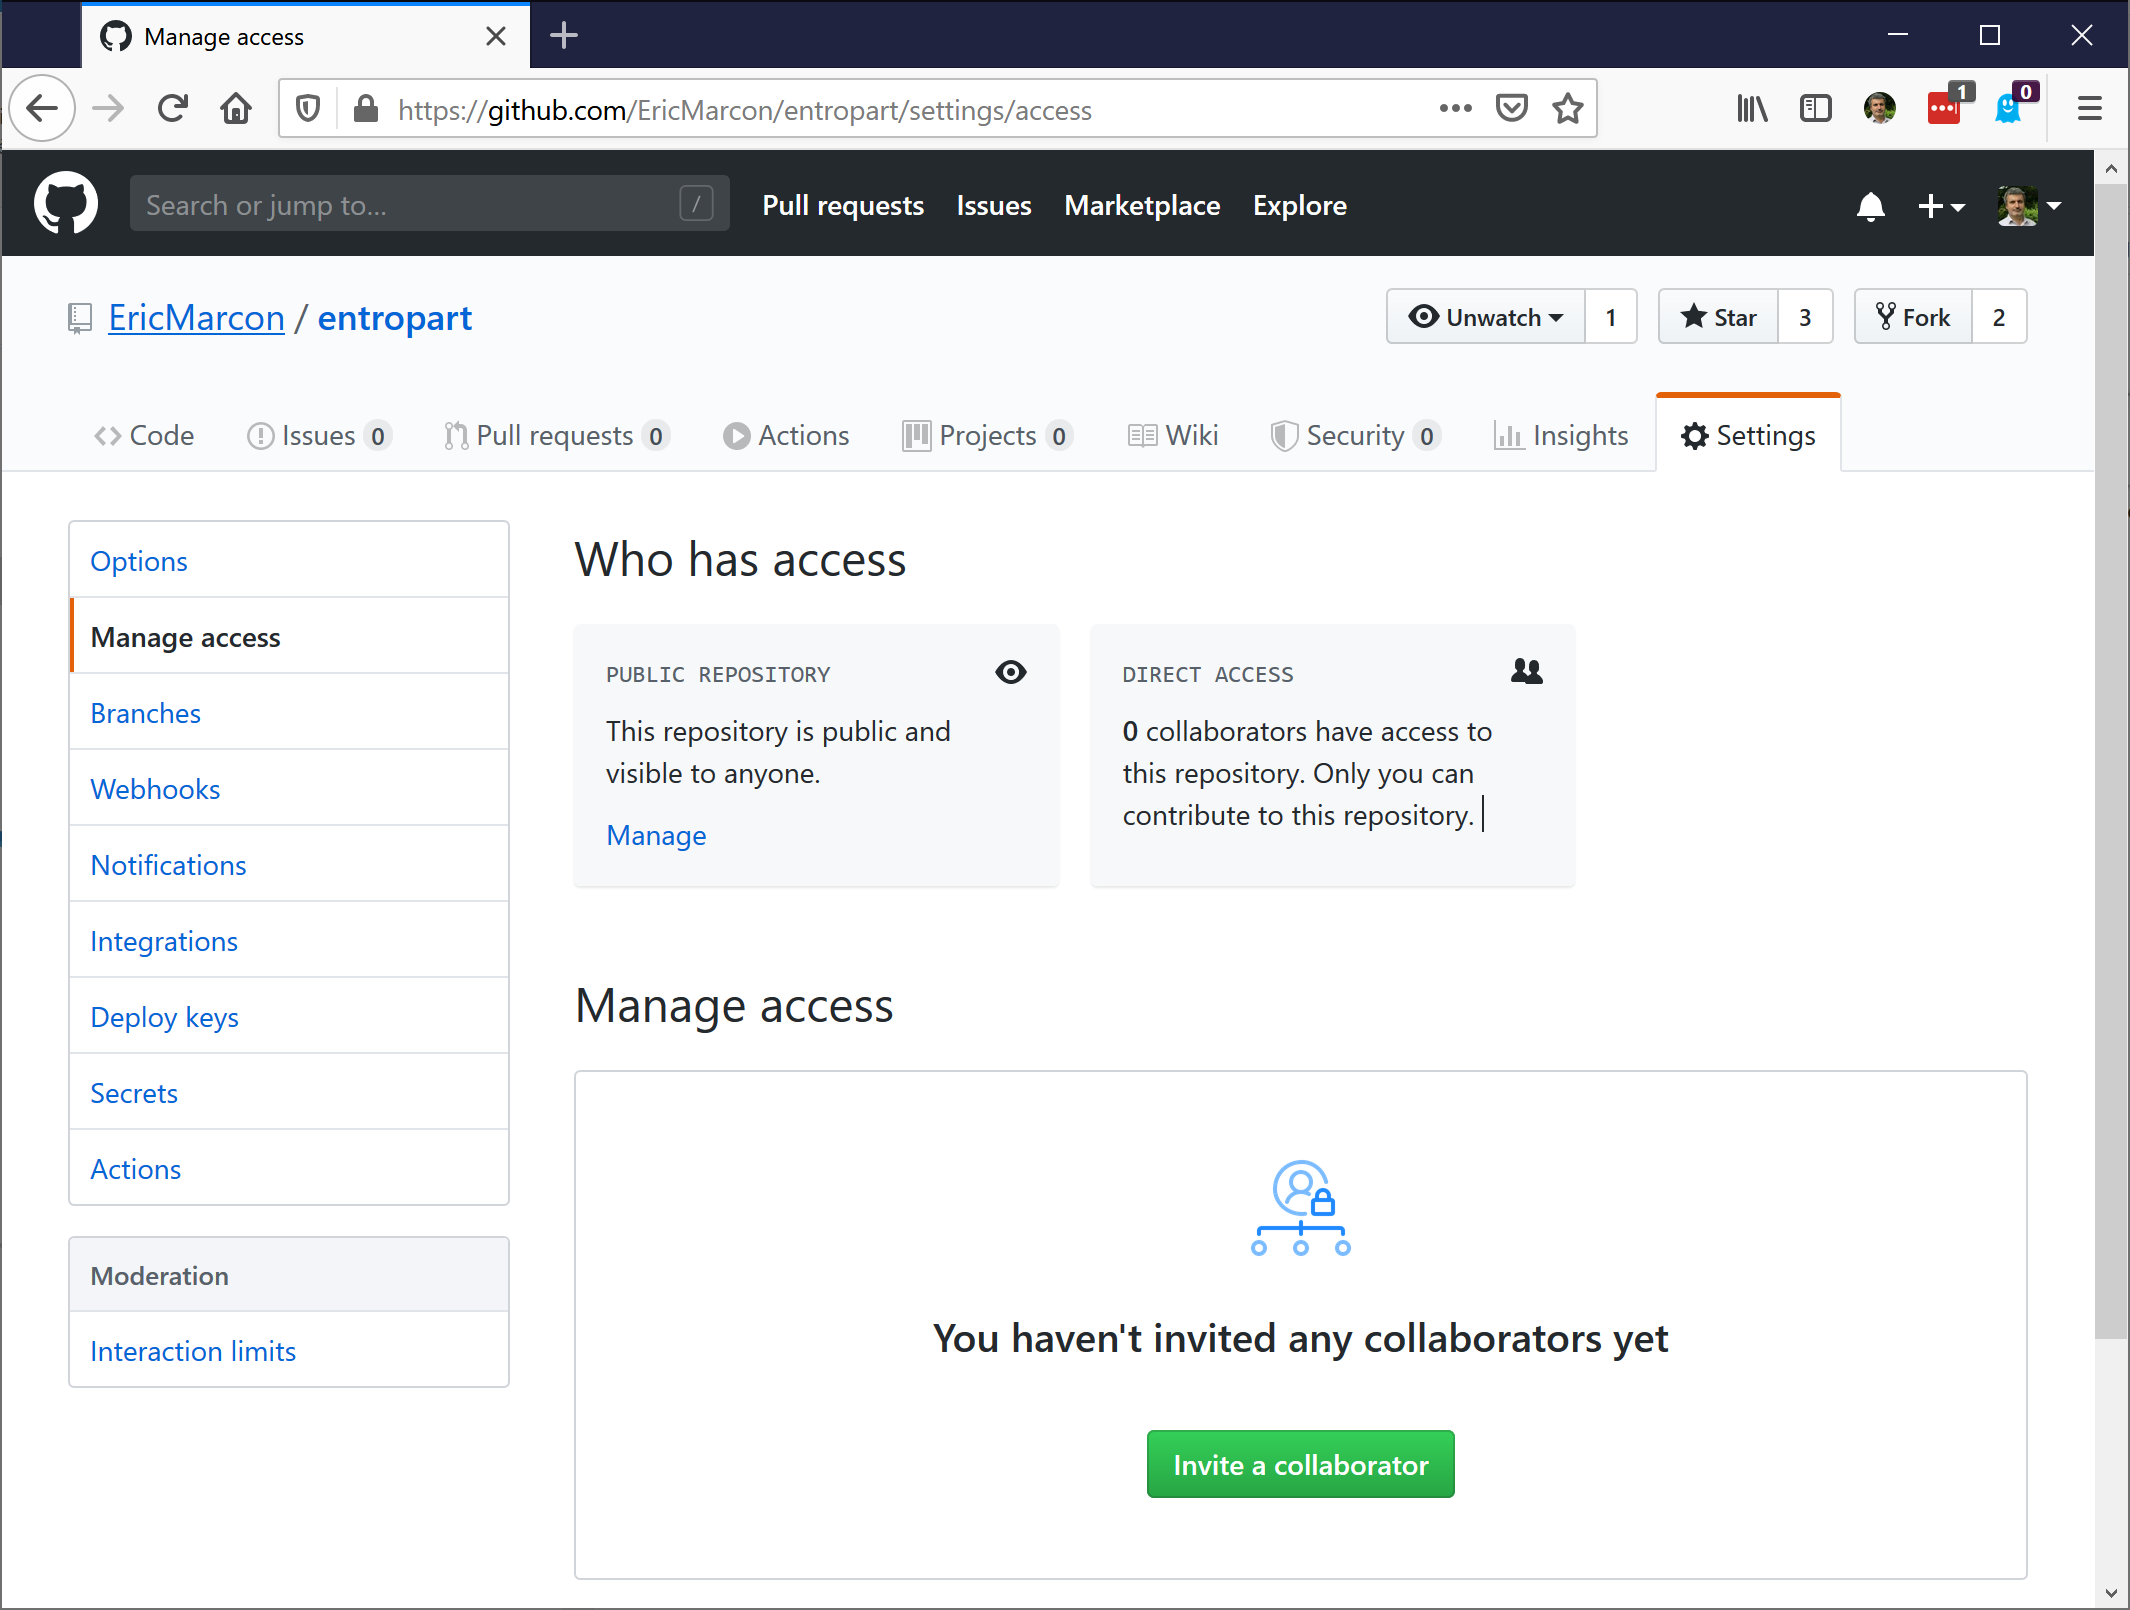
\includegraphics[width=0.8\linewidth]{images/git-Access} 

}

\caption{Assigning access rights on GitHub.}\label{fig:git-Access}
\end{figure}

\normalsize

Collaborators are invited by a message sent by \emph{GitHub}.

\section{Common usage}\label{common-usage}

\subsection{Pull, modify, commit, push}\label{pull-modify-commit-push}

Any work session on a project starts by pulling (\enquote{Pull} button) from the \emph{Git} window to integrate to the local repository the updates made on GitHub by other collaborators.

The changes made to the project files are then taken into account (check the \enquote{Staged} boxes) and committed with an explanatory message.
A good practice is to validate changes each time an elementary task which can be described in the explanatory message is completed rather than making \emph{commits} that group many changes with a vague description.

As soon as possible, \emph{Push} updates so that they are visible to collaborators.

\subsection{Resolve conflicts}\label{resolve-conflicts}

It is not possible to push validated changes if a collaborator has modified the remote repository on GitHub.
In this case, you have to pull them to the local repository before pushing the merged changes.

A conflict occurs if a \emph{Pull} imports a change into the local file that cannot be merged automatically because a conflicting change occurred locally.
Git considers each line to be indivisible: changing the same line in the remote repository and the local repository therefore generates a conflict.

Git inserts both versions in the file containing a conflict with a particular presentation:

\begin{verbatim}
<<<<<<<<< HEAD # Imported version of the conflict
Lines in conflict, imported version
========= # boundary between the two versions
Lines in conflict, local version
>>>>>>>>> # End of conflict
\end{verbatim}

The formatting lines containing the \texttt{\textless{}\textless{}\textless{}\textless{}}, the \texttt{====} and the \texttt{\textgreater{}\textgreater{}\textgreater{}\textgreater{}} must be deleted and only one version of the problematic lines kept, which can be different from the two original versions.
The conflict resolution must be taken into account and validated.

To limit conflicts in a document containing text (typically, an R Markdown document), a good practice is to treat each sentence as a line, terminated by a line break that will not be visible in the formatted document: two line breaks are required to separate paragraphs.

\subsection{See the differences}\label{see-the-differences}

In the RStudio \emph{Git} window, the context menu (displayed by right-clicking) \enquote{Diff} can be used to display the changes made to each file (figure \ref{fig:git-diff}).



\scriptsize

\begin{figure}

{\centering 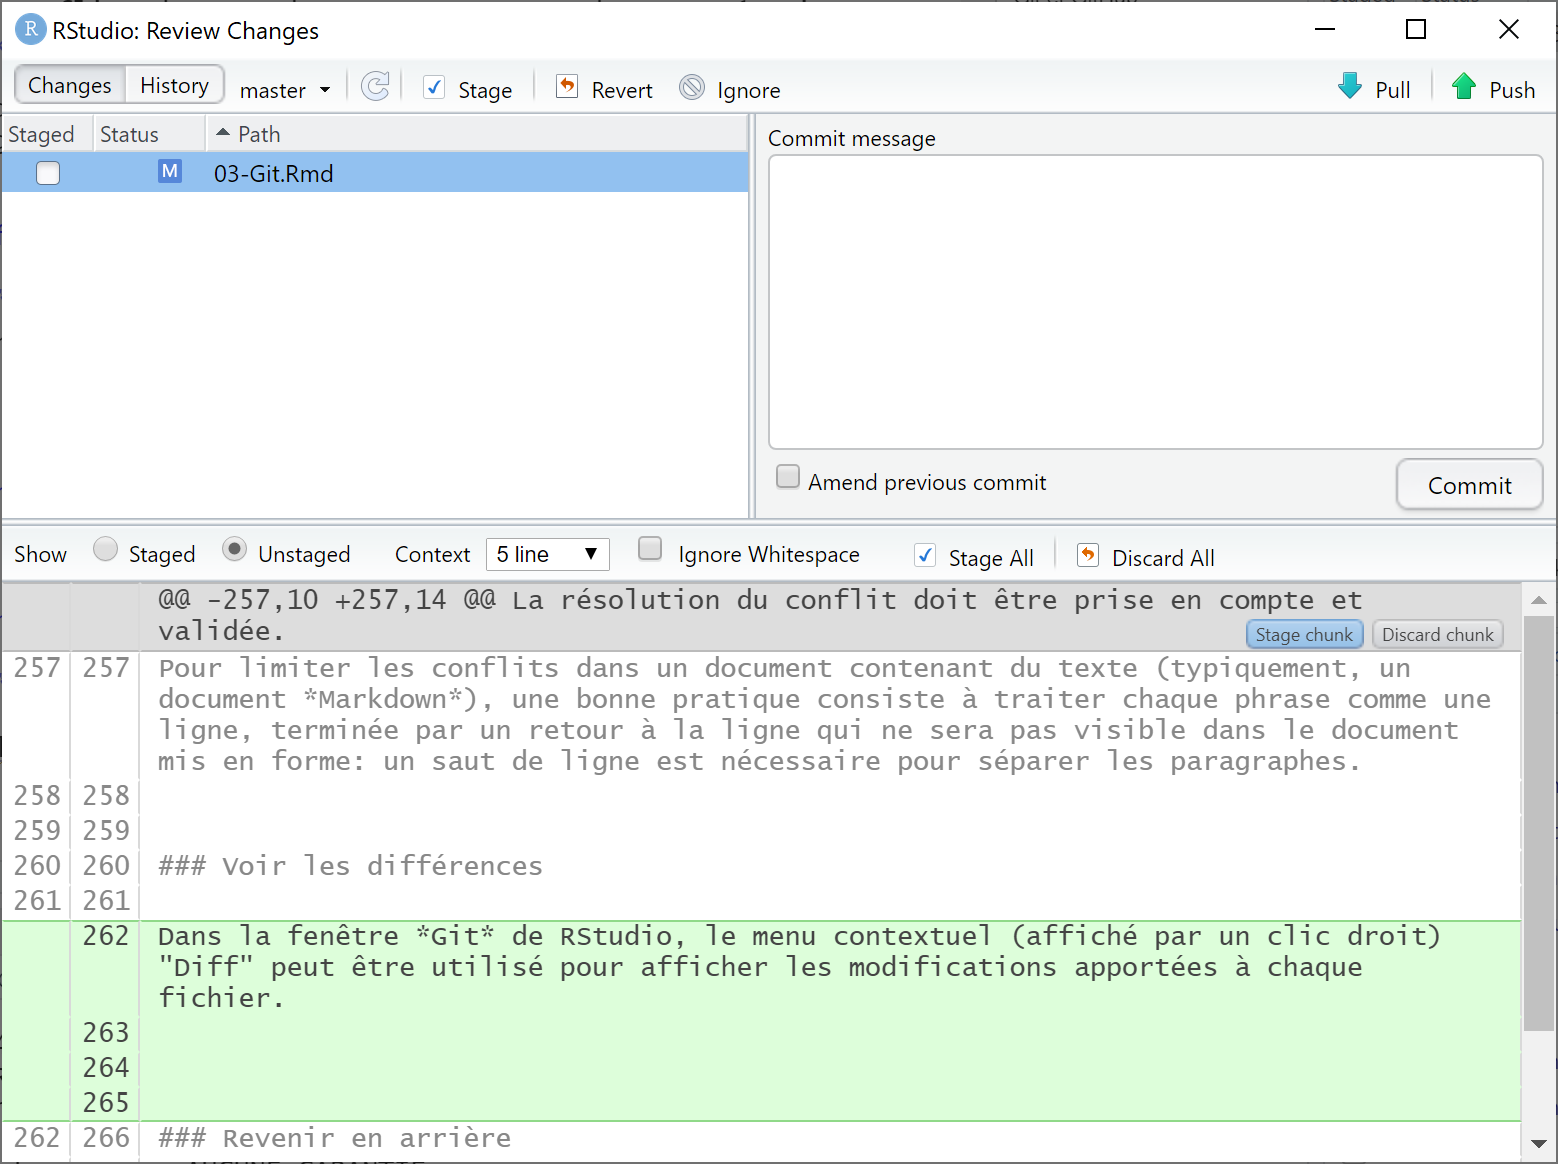
\includegraphics[width=0.8\linewidth]{images/git-diff} 

}

\caption{Differences between the working directory and the head.}\label{fig:git-diff}
\end{figure}

\normalsize

\subsection{Revert}\label{revert}

The contextual menu \enquote{Revert} allows you to undo all the modifications made to a file (displayed by \emph{Diff}) and to restore its content validated the last time (its state in the head).

It is not easy to go back beyond the last validation because the modifications may have been taken into account by collaborators: deleting them would make the project incoherent.

\subsection{View history}\label{view-history}

The clock-shaped button in the RStudio \emph{Git} window displays the history of the project (figure \ref{fig:git-history}).



\scriptsize

\begin{figure}

{\centering 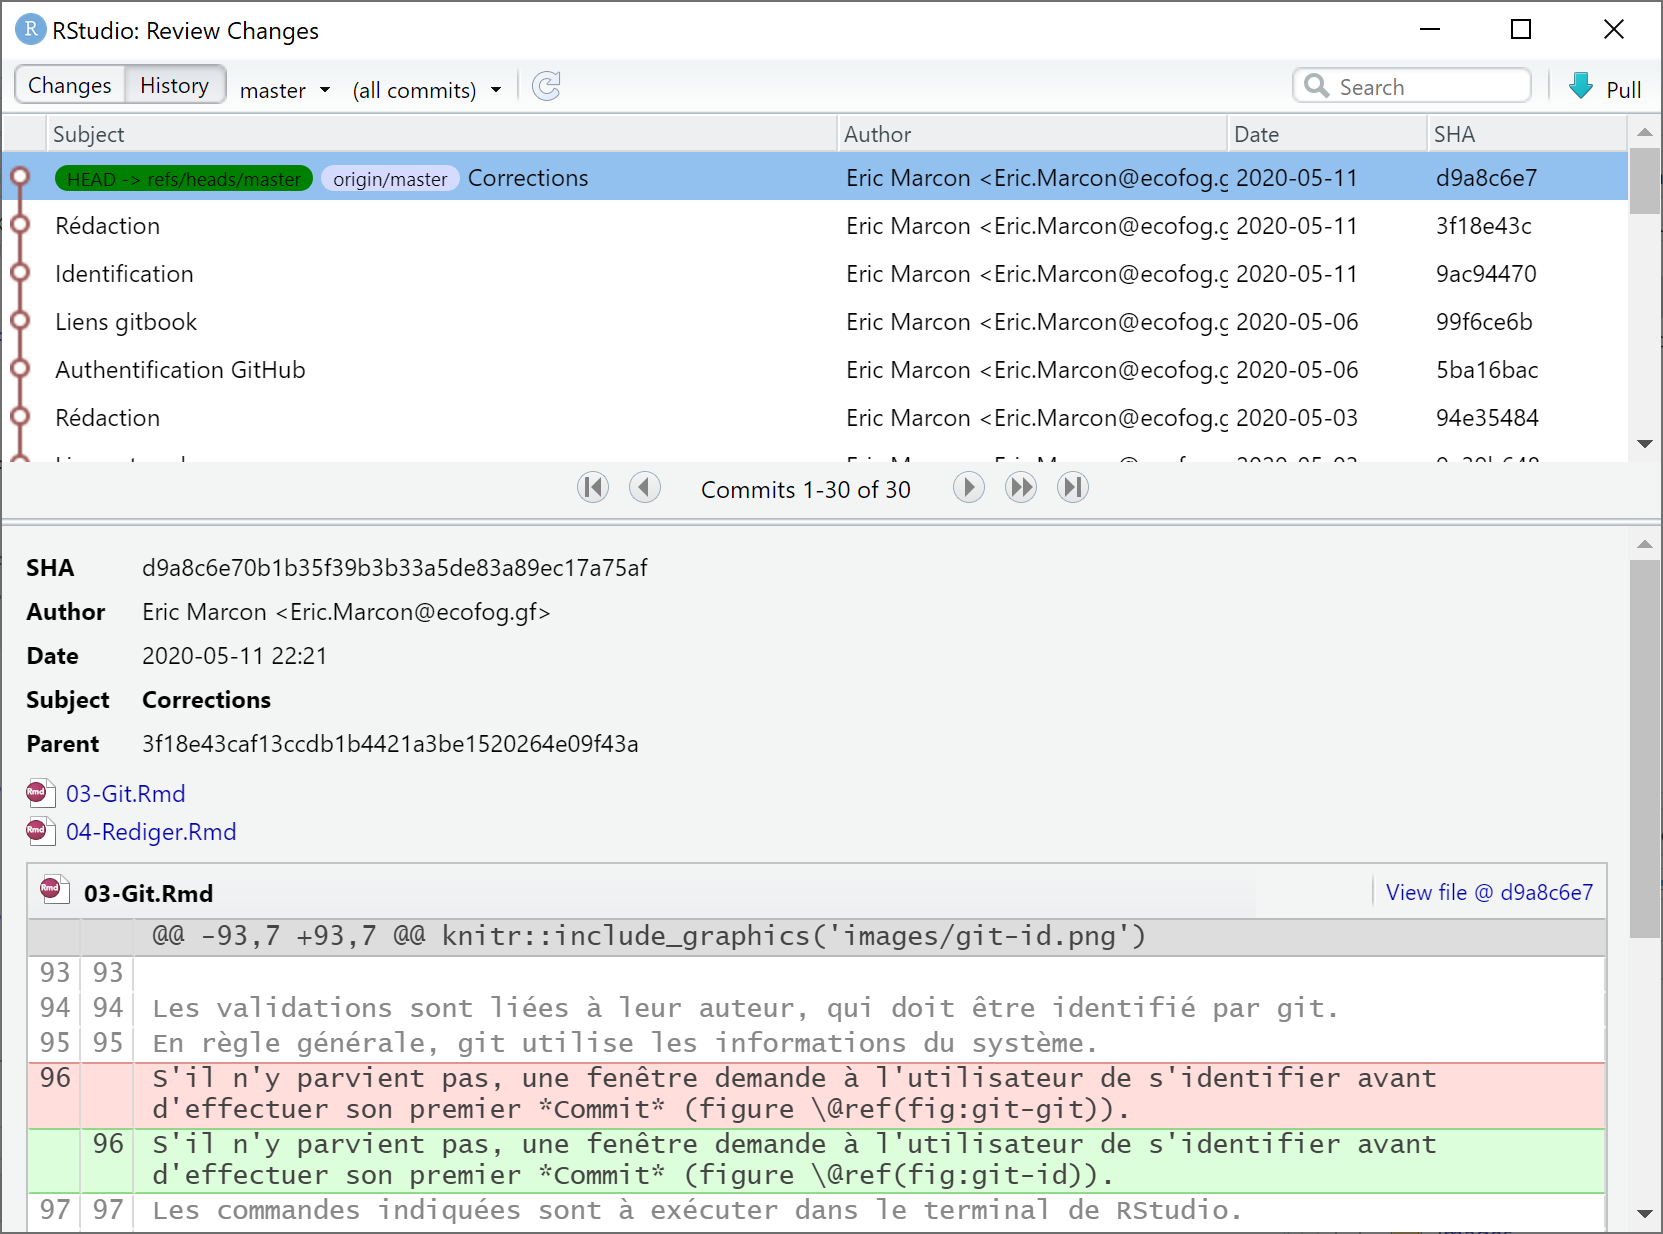
\includegraphics[width=0.8\linewidth]{images/git-historique} 

}

\caption{History of commits in the repository.}\label{fig:git-history}
\end{figure}

\normalsize

At the top is the head, and then all the commits that made it up.
For each validation, the differences of each file can be displayed by clicking on the file name in the lower part of the window.

\section{Branches}\label{sec:branches}

The branches of a project are different but simultaneous versions.
A typical use is the development of a new feature.
If it takes a long time to write, the project is disturbed by the current work in progress: the code may not work anymore.
If the development turns out to be impossible or useless, it must be abandoned without damage.
In order to isolate it during its development and to be able to validate or abandon it at the end, it must be placed in a branch.

The main branch of the project is called \enquote{master} or \enquote{main} from November 2020\footnote{\url{https://github.com/github/renaming}}.
It must always be in a stable state: it is the one that is cloned from GitHub by other possible users.

The change of convention for the name of the \enquote{master} branch means that from November 2020, projects created on GitHub cloned in RStudio have the main branch \enquote{main} while projects created on RStudio and then linked to GitHub keep the \enquote{master} name.

\subsection{Create a new branch}\label{create-a-new-branch}

Click on the purple \enquote{New Branch} button in the RStudio \emph{git} window.
Enter its name and click on \enquote{Create}.

The new branch is now active.

The git commands can also be run in the terminal (to create the branch and activate it):

\begin{verbatim}
git branch new_branch
git checkout new_branch
\end{verbatim}

\subsection{Change branch}\label{change-branch}

Select the branch to activate from the list of local branches in the \emph{git} window.

The \emph{commits} apply to the active branch.
Each branch behaves as a different version of the project.

Warning: to avoid confusion, save the changes, stage them and commit them before changing branch.

\subsection{Pushing the new branch}\label{pushing-the-new-branch}

The first modifications of the new branch must be pushed with the command line because the \enquote{Push} and \enquote{Pull} buttons of the \emph{Git} window do not work as long as the branch does not exist on the remote repository.

Run, in the terminal:

\begin{verbatim}
git push -u origin new_branch
\end{verbatim}

\subsection{Filesystem behavior}\label{filesystem-behavior}

Each time a branch changes, git rewrites the project files to reflect the state of the branch.
The changes can be seen outside of RStudio, in the file browser for example.

Files ignored by \texttt{.gitignore} are not changed.
It is therefore essential that the \texttt{.gitignore} files in the different branches are identical, otherwise files ignored in one branch will appear as added in the displayed branch after a change.

Development branches have a content close to that of the main branch.
This is not the case with specialized branches seen later, such as \texttt{gh-pages} (see section \ref{sec:github-pages}) which contains the repository's presentation web site.
It is best not to attempt to display these branches in RStudio: their content is produced automatically and should not be modified manually.
If it is necessary, it will be necessary to copy the \texttt{.gitignore} file of the main branch and keep in mind that the ignored files actually belong to another branch than the one displayed.

\subsection{\texorpdfstring{Merge with \texttt{merge}}{Merge with merge}}\label{merge-with-merge}

Merging a development branch with the main branch marks the achievement of its goal: its code will be integrated into the project.
RStudio's GUI does not allow for merging, so you have to use the terminal: first, go to the target branch (possible with the GUI):

\begin{verbatim}
git checkout master
\end{verbatim}

Then, merge:

\begin{verbatim}
git merge new_branch
\end{verbatim}

In most situations, the merge will be automatic (\enquote{Fast Forward}).
It is possible that conflicts appear: use the \texttt{git\ status} command to display the list of files concerned, open them, resolve the conflict and perform a \emph{commit}.

The merged branch is not deleted: it can be used again for further development or deleted manually with the following command:

\begin{verbatim}
git branch -d new_branch
\end{verbatim}

\subsection{Merging with a pull request}\label{merging-with-a-pull-request}

The other way of merging is more formal but also more general: it allows you to merge a branch into another user's repository to contribute to it, or to have your branch validated by another team member in a collaborative project.

To contribute to another GitHub user's project\footnote{\url{https://git-scm.com/book/fr/v2/GitHub-Contribution-\%C3\%A0-un-projet}}, you have to start by creating a \emph{fork} of it, i.e.~a copy in the form of a repository linked to the original.
It will be possible to pull changes from the original to stay up to date\footnote{\url{https://ardalis.com/syncing-a-fork-of-a-github-repository-with-upstream/}} (as opposed to a simple snapshot copy made by downloading a zip of the project) and, at the end of the development, to merge the \emph{fork} to the original repository (as opposed to a clone that would not allow to contribute afterwards).

Next, create a development branch as before, modify it and finally ask the repository owner to merge it.
This process is described in detail in the git documentation.

In the simpler case of a branch of one's own project as in the case of a \emph{fork}, the development branch is ready to be merged.
It must have been pushed on GitHub.
On the GitHub page of the project, a \enquote{Create Pull Request} button allows to request the merge.
A message describing the proposed changes with their arguments must be added.

The owner of the project (the team members in the case of a collaborative project, or yourself if the team is reduced to one person) is notified of the pull request.
On the original project page, it is possible to see the message, the list of modifications (chronology of \emph{commits} or comparison of files), to start a discussion with the author of the request\ldots{}
If the request is not accepted, it can be closed.
If it is validated, the \enquote{Merge Pull Request} button allows to merge the development branch with the \enquote{master} branch (or another one) of the source project.

Pull requests are the only way to contribute to a repository on which you don't have write rights.
It is also the way to merge a development branch into your own project by keeping an explicit trace of it (in the \emph{Pull requests} section of the project's GitHub page).
In a collaborative project, the proposals of a member (author of the request) can be validated by another (who accepts the merge).

\section{Advanced usage}\label{advanced-usage}

\subsection{Git commands}\label{git-commands}

Beyond the common use allowed by the RStudio graphical interface, advanced manipulations of projects are allowed by using git in command line.
Some useful examples are presented here.

A short guide of commands is proposed by Roger Dudler\footnote{\url{https://rogerdudler.github.io/git-guide/index.fr.html}}.
It summarizes the essential commands, thus integrated in the graphical interface of RStudio.
Links to more complete references are given at the bottom of the page.

\subsection{Size of a repository}\label{size-of-a-repository}

To find out how much disk space a repository occupies, use the command \texttt{git\ count-objects\ -vH}\footnote{\url{https://git-scm.com/docs/git-count-objects}}.

The data for this document at the time of writing is presented as an example.

\begin{verbatim}
$ git count-objects -v
count: 200
size: 2.66 MiB
in-pack: 0
packs: 0
size-pack: 0
prune-packable: 0
garbage: 0
size-garbage: 0
\end{verbatim}

The total size is on the \emph{size} line.
Packs are a method used by git to reduce the size of the repository: similar files are stored as a common part and differences.
The \emph{prune-packable} line gives the size of objects stored both individually and in packs.
If their size is large, run \texttt{git\ prune-packed} to reduce it to zero.

The \emph{size-garbage} line gives the size of objects that can be deleted.
\texttt{git\ gc} removes them, but not only that: it optimizes storage.

\begin{verbatim}
git gc
Enumerating objects: 194, done.
Counting objects: 100% (194/194), done.
Delta compression using up to 8 threads
Compressing objects: 100% (188/188), done.
Writing objects: 100% (194/194), done.
Total 194 (delta 83), reused 0 (delta 0)

$ git count-objects -vH
count: 1
size: 5.72 KiB
in-pack: 194
packs: 1
size-pack: 4.00 MiB
prune-packable: 0
garbage: 0
size-garbage: 0 bytes
\end{verbatim}

Here, the majority of the objects in the repository have been placed in a pack (but its size is larger than the individual objects).

There is usually no need to do garbage collection manually: git handles the organization of its repositories well.

GitHub limits the size of repositories.
As of May 2020, the limit is 100 GB.
The size of all repositories of an authenticated user can be displayed in his account settings (\enquote{Personal Settings}, \enquote{Repositories})\footnote{\url{https://github.com/settings/repositories}}.

\subsection{Delete a folder}\label{delete-a-folder}

All changes made to a repository are stored in its history.
It can be useful to delete them in some particular cases

\begin{itemize}
\tightlist
\item
  if a file containing confidential information was inadvertently committed.
  Committing its deletion does not remove it from the history, and the confidential information remains visible when consulting the history.
\item
  if large files are no longer needed, e.g.~PDF files produced by R Markdown (chapter \ref{chap-rediger}) which are binary (thus unsuitable for git) and reproducible from the code.
\end{itemize}

Typically, the \texttt{docs} folder is used to store documents produced from R Markdown code.
The HTML and PDF files must be in this folder to constitute the GitHub pages of the project.
Each modification of the repository generates a new version of these files whose history volume quickly becomes huge.
An efficient solution is to delegate the creation of these files to a continuous integration system (chapter \ref{chap-ci}) and to remove the \texttt{docs} folder from the main branch (\emph{master}) of the repository.
You then have to delete all its history to recover the space it occupies, which can be most of the size of the repository.

The commands to completely delete a folder from a repository are presented here\footnote{\url{https://stackoverflow.com/questions/10067848/remove-folder-and-its-contents-from-git-githubs-history}}.
The repository must be clean, i.e.~without unvalidated changes, and the remote and local versions synchronized.

The following three commands completely remove the \texttt{docs} folder from the git repository history:

\begin{verbatim}
git filter-branch --tree-filter "rm -rf docs" |>
    --prune-empty HEAD
git for-each-ref --format="%(refname)" refs/original/ |>
    | xargs -n 1 git update-ref -d
\end{verbatim}

The \texttt{docs} folder is not removed from the working directory.
It must therefore be added to the \texttt{.gitignore} file so that it is no longer tracked.
The modification of \texttt{.gitignore} must be validated.
These operations can be done with the RStudio interface or on the command line:

\begin{verbatim}
echo docs/ >> .gitignore
git add .gitignore
git commit -m 'Removing docs folder from git history'
\end{verbatim}

The repository cleanup is necessary to physically remove the removed data:

\begin{verbatim}
git gc
\end{verbatim}

Finally, the repository must be pushed.
The \texttt{-\/-force} option involves replacing the contents of the remote repository with those of the local repository: all changes made by collaborators are erased, so this cleanup operation involves suspending the development of the project while it takes place.

\begin{verbatim}
git push origin master --force
\end{verbatim}

This code can be used to completely remove any file or folder from a repository by simply replacing \texttt{docs} in the initial \texttt{git\ filter-branch} command.
The reduction in repository size can be tracked using \texttt{git\ count-objects\ -vH} before the operation, before \texttt{git\ gc} (the repository size remains stable but has been moved to \emph{garbage}) and at the end (the repository size is significantly reduced).

\subsection{Revert}\label{revert-1}

It is possible to restore a repository to a previous state by placing its head (figure \ref{fig:git-Trees}) at the level of an old \emph{commit}.
All subsequent modifications are then destroyed.
This operation should not be performed on a shared repository: other users would not be able to push their modifications anymore.

Display the repository history and look for the identifier (SHA) of the last \emph{commit} to keep.
In the RStudio terminal, run:

\begin{verbatim}
git reset --hard <SHA>
git push -f
\end{verbatim}

All repository history after the chosen restore point is lost.

A less drastic method that can be used on a shared repository is to perform a \emph{commit} that undoes another's changes but does not destroy any history data.
This operation only undoes one \emph{commit} at a time, so it must be repeated to undo several, starting with the most recent.
In the RStudio terminal, run:

\begin{verbatim}
git revert <SHA>
\end{verbatim}

To undo the last \emph{commit}, execute:

\begin{verbatim}
git revert HEAD
\end{verbatim}

Using \texttt{HEAD} simply avoids searching for the corresponding ID.

\section{Confidential data in a public repository}\label{sec:confidential}

A public repository on GitHub causes problems when the data used in the project is not.

An unsatisfactory solution is to not include the data in the project, which makes it non-reproducible.
A better solution is to encrypt them, allowing some users to decrypt them.
This is the purpose of the \textbf{secret} package.

A safe (\texttt{vault} folder) is created in the project.
It contains a list of authorized users: each of them must have a pair of encryption keys, a public key included in the safe and a private key, kept secret.
The data is encrypted with all the public keys available (and therefore duplicated).
The users then each use their own private key for decryption.

To avoid duplicating data, the repository owner should create a generic user for the project, whose private key he will communicate outside GitHub.
The vault will contain the keys of the project owner and the generic user only.
If the generic user's private key is compromised, it will be sufficient to remove it from the vault and create a new one.

\subsection{Generating a key pair for the project owner}\label{generating-a-key-pair-for-the-project-owner}

The keys are generated by the \emph{ssh} software, installed with \emph{git} or by default on Linux.

The procedure is the same as in the section \ref{sec:SSH}, but the key used must be in RSA format (supported by the \textbf{secret} package, as opposed to the more secure ed25519 format used for authentication on GitHub).

Run the following command in the RStudio terminal to create an RSA key:

\begin{verbatim}
ssh-keygen -t rsa -b 4096 -C "user.email"
\end{verbatim}

Store the public key on GitHub in \enquote{Settings \textgreater{} SSH and GPG Keys}.
Note the position of the key: if an authentication key has already been stored for two workstations for example, the RSA key will be the third one.

\subsection{Generating a key pair for the project}\label{generating-a-key-pair-for-the-project}

Generate a key in RSA format in the RStudio terminal:

\begin{verbatim}
ssh-keygen -t rsa -b 4096" 
\end{verbatim}

\begin{itemize}
\tightlist
\item
  Enter the name of the key: \texttt{\textless{}RepoID\textgreater{}.rsa}.
\item
  Do not enter a passphrase to allow the key to be used without interaction.
\end{itemize}

The private key \texttt{\textless{}RepoID\textgreater{}.rsa} should only be distributed to the rightful owners of the project.
You must therefore add the line \texttt{*.rsa} to the \texttt{.gitignore} file of the project to avoid pushing the key on GitHub.

To allow the continuous integration of the project (chapter \ref{chap-ci}), the private key must be stored as a secret of the GitHub repository containing the project.
Apply the procedure in section \ref{sec:secrets-ci} to create a secret named \enquote{RSA} and paste the content of the file \texttt{\textless{}RepoID\textgreater{}.rsa} in the \enquote{Value} field of the form.

The use of the secret is described in section \ref{sec:secrets-ci}.

\subsection{Creating a safe}\label{creating-a-safe}

Execute:

\scriptsize

\begin{Shaded}
\begin{Highlighting}[]
\FunctionTok{library}\NormalTok{(}\StringTok{"secret"}\NormalTok{)}
\NormalTok{vault }\OtherTok{\textless{}{-}} \StringTok{"vault"}
\FunctionTok{create\_vault}\NormalTok{(vault)}
\end{Highlighting}
\end{Shaded}

\normalsize

\subsection{Adding users}\label{adding-users}

The owner of the project is added from his public key stored on GitHub, which is the third one in our example.

\scriptsize

\begin{Shaded}
\begin{Highlighting}[]
\CommentTok{\# GitHub ID of the project owner}
\NormalTok{github\_user }\OtherTok{\textless{}{-}} \StringTok{"EricMarcon"}
\CommentTok{\# Read and store the key, i is the key number}
\FunctionTok{add\_github\_user}\NormalTok{(github\_user, }\AttributeTok{vault =}\NormalTok{ vault, }\AttributeTok{i =} \DecValTok{3}\NormalTok{)}
\end{Highlighting}
\end{Shaded}

\normalsize

The generic project user's key is added by:

\scriptsize

\begin{Shaded}
\begin{Highlighting}[]
\FunctionTok{library}\NormalTok{(}\StringTok{"openssl"}\NormalTok{)}
\NormalTok{project\_id }\OtherTok{\textless{}{-}} \StringTok{"ProjectName"}
\CommentTok{\# Read the key}
\NormalTok{rsa\_project }\OtherTok{\textless{}{-}} \FunctionTok{read\_pubkey}\NormalTok{(}\FunctionTok{paste0}\NormalTok{(project\_id, }\StringTok{".rsa.pub"}\NormalTok{))}
\CommentTok{\# Add to the vault}
\FunctionTok{add\_user}\NormalTok{(project\_id, }\AttributeTok{public\_key =}\NormalTok{ rsa\_project, }\AttributeTok{vault =}\NormalTok{ vault)}
\end{Highlighting}
\end{Shaded}

\normalsize

\subsection{Storing the data}\label{storing-the-data}

The data, stored in R variables, are stored one by one by the \texttt{add\_secret()} function.
In the following example, the variable is called \texttt{X} and equals 1.

\scriptsize

\begin{Shaded}
\begin{Highlighting}[]
\NormalTok{X }\OtherTok{\textless{}{-}} \DecValTok{1}
\FunctionTok{add\_secret}\NormalTok{(}
  \CommentTok{\# Name of the data}
  \StringTok{"X"}\NormalTok{, }
  \CommentTok{\# Value}
  \AttributeTok{value =}\NormalTok{ X, }
  \CommentTok{\# Authorized users: owner and generic}
  \AttributeTok{users =} \FunctionTok{c}\NormalTok{(}\FunctionTok{paste0}\NormalTok{(}\StringTok{"github{-}"}\NormalTok{, github\_user), project\_id), }
  \CommentTok{\# Vault}
  \AttributeTok{vault =}\NormalTok{ vault}
\NormalTok{)}
\end{Highlighting}
\end{Shaded}

\normalsize

The contents of the vault can be checked:

\scriptsize

\begin{Shaded}
\begin{Highlighting}[]
\CommentTok{\# List of vault data}
\FunctionTok{list\_secrets}\NormalTok{(}\AttributeTok{vault =}\NormalTok{ vault)}
\end{Highlighting}
\end{Shaded}

\begin{verbatim}
##   secret        email
## 1      X github-E....
\end{verbatim}

\begin{Shaded}
\begin{Highlighting}[]
\CommentTok{\# List of owners of the data "X}
\FunctionTok{list\_owners}\NormalTok{(}\StringTok{"X"}\NormalTok{, }\AttributeTok{vault =}\NormalTok{ vault)}
\end{Highlighting}
\end{Shaded}

\begin{verbatim}
## [1] "github-EricMarcon" "ProjectName"
\end{verbatim}

\normalsize

The data will be read into the project code by the \texttt{get\_secret()} command.
The private key of the generic project user, communicated by a secure means to the owners, must be in the project folder.

\scriptsize

\begin{Shaded}
\begin{Highlighting}[]
\CommentTok{\# Select the private key}
\FunctionTok{Sys.setenv}\NormalTok{(}\AttributeTok{USER\_KEY =}\NormalTok{ usethis}\SpecialCharTok{::}\FunctionTok{proj\_path}\NormalTok{(}\FunctionTok{paste0}\NormalTok{(project\_id, }\StringTok{".rsa"}\NormalTok{)))}
\CommentTok{\# Read the data "X}
\FunctionTok{get\_secret}\NormalTok{(}\StringTok{"X"}\NormalTok{, }\AttributeTok{vault =}\NormalTok{ vault)}
\end{Highlighting}
\end{Shaded}

\begin{verbatim}
## [1] 1
\end{verbatim}

\normalsize

The key can be verified:

\scriptsize

\begin{Shaded}
\begin{Highlighting}[]
\FunctionTok{local\_key}\NormalTok{()}
\end{Highlighting}
\end{Shaded}

\begin{verbatim}
## [4096-bit rsa private key]
## md5: e81dcb0745a755286c2dc1fc4c6ad117
## sha256: cca11ef82e17c3b77b699e7f3c23e083e8f0f79cb70be8274799f076c44b0c2d
\end{verbatim}

\normalsize

\section{GitHub pages}\label{sec:github-pages}

Any project on GitHub must have contained a \texttt{README.md} file to present it.
This file is written in Markdown format.

The file can be placed in the \texttt{docs} folder to provide both the repository's home page and its website.
The \textbf{memoiR} package provides commands to automate these tasks in document projects.
A repository containing an article written in R Markdown (see section \ref{sec:memo}) is used as an example\footnote{\url{https://github.com/EricMarcon/Krigeage}}.

Its \texttt{README.md} file exists in both locations: it is written by the developer at the root of the project and duplicated in \texttt{docs}.

\subsection{Activation}\label{activation}

To activate GitHub pages, you have to open the repository settings and modify the \enquote{GitHub Pages} item (in \enquote{Options}).
Select the project branch and the folder containing the web pages, here: \texttt{master} and \texttt{/docs}.
As an option, choosing a theme customizes the appearance of the pages.

The web site is accessible at an address\footnote{\url{https://EricMarcon.github.io/Krigeage/}} of the domain \emph{github.io}.

The \texttt{README.md} file displayed on the home page has a very different look but the same content as the one displayed with the code on the repository page in GitHub.

The interest of the GitHub pages is to allow an easy access to the formatted documents when the repository contains a written production or to the documentation of R packages.
These contents will be presented in the next chapter.

A main website is proposed with each GitHub account, at \url{https://GitHubID.github.io}\footnote{Example: \url{https://EricMarcon.github.io/Krigeage/}}.
It will be used to host a personal website produced by \textbf{blogdown}.

\subsection{Badges}\label{badges}

Badges are small images, possibly dynamically updated, that provide quick information about the status of a project.
They should be placed immediately after the title of the \texttt{README.md} file.

A good practice is to indicate the progress in the life cycle of the project.
The corresponding badges are listed on the Tidyverse site\footnote{\url{https://www.tidyverse.org/lifecycle/}}.

Their Markdown code is as follows:

\begin{verbatim}
![stability-wip]
(https://img.shields.io/badge/lifecycle-maturing-blue.svg)
\end{verbatim}

The \textbf{usethis} package simplifies their creation by placing the necessary code in the clipboard.
Then just paste it into the file.

\scriptsize

\begin{Shaded}
\begin{Highlighting}[]
\NormalTok{usethis}\SpecialCharTok{::}\FunctionTok{use\_lifecycle\_badge}\NormalTok{(}\StringTok{"maturing"}\NormalTok{)}
\end{Highlighting}
\end{Shaded}

\normalsize

\chapter{Writing}\label{chap-rediger}

\toc{1}

R and RStudio make it possible to efficiently write documents of all formats, from simple notepads to theses to slide shows.
The tools to do this are the subject of this chapter, completed by the production of web sites (including a personal site).

Two document production processes are available:

\begin{itemize}
\tightlist
\item
  \emph{R Markdown} with the \textbf{knitR} and \textbf{bookdown} packages.
  This is the classic method, presented here in detail.
\item
  \emph{Quarto}, designed to be used with languages beyond R and in working environments beyond RStudio.
  Quarto is under active development but does not yet allow documents to be produced with the same quality as \emph{R Markdown}: for example, punctuation in French documents is not handled correctly in PDF\footnote{\url{https://github.com/jgm/pandoc/issues/8283/}}, tables cannot include equations\footnote{\url{https://github.com/quarto-dev/quarto-cli/issues/555}} and the width of figures is inconsistent in PDF documents formatted with several columns\footnote{\url{https://github.com/quarto-dev/quarto-cli/issues/855}}.
  The use of Quarto is well documented on its site\footnote{\url{https://quarto.org/}} and is not presented here.
\end{itemize}

\section{Markdown notebook (R Notebook)}\label{markdown-notebook-r-notebook}

In an \texttt{.R} file, the code should always be commented to make it easier to read.
When the explanation of the code requires several lines of comment per line or block of code, it is time to reverse the logic and place the code in the text.

The concept of literate programming was developed by \textcite{Knuth1984}.
It consists in describing the objectives and methods by text, in which the code is integrated.

The simplest tool is the Markdown notebook (Menu \enquote{File \textgreater{} New File \textgreater{} R Notebook}).
The document template contains its instructions for use.

The language for formatting the text is Markdown\footnote{\url{https://fr.wikipedia.org/wiki/Markdown}}, an easy to use markup language:

\begin{itemize}
\tightlist
\item
  Paragraphs are separated by line breaks.
\item
  The document is structured by headings: their line starts with a number of \texttt{\#} corresponding to their level.
\item
  Character formats are limited to the essentials: italic or bold (text surrounded by one or two \texttt{*}).
\item
  Other simple codes allow all useful formatting.
\end{itemize}

This language is the core of the pandoc\footnote{\url{https://fr.wikipedia.org/wiki/Pandoc}} software, dedicated to converting documents of different formats.

The \textbf{rmarkdown} package \autocite{Xie2015} bridges the gap between R and Markdown, relying on the RStudio interface which is not essential but greatly simplifies its use.
The Markdown dialect used by the package is called \emph{R Markdown}.
Its syntax is summarized in a cheat sheet\footnote{\url{https://rstudio.com/wp-content/uploads/2015/02/rmarkdown-cheatsheet.pdf}}.
Its complete documentation is online \autocite{Xie2018}.

Equations are written in the LaTeX format\footnote{\url{https://fr.wikibooks.org/wiki/LaTeX/\%C3\%89crire_des_math\%C3\%A9matiques}}.

The simplest organization of a \emph{R Markdown} document can be seen in the notepad template.
It starts with a header in YAML format\footnote{\url{https://fr.wikipedia.org/wiki/YAML}}:

\begin{verbatim}
---
title: "R Notebook"
output: html_notebook
---
\end{verbatim}

The first entry is the title, the second is the output format: more precisely the name of the function that will process the document.

The document contains Markdown formatted text and code chunks surrounded by three backquotes (the Markdown syntax of a code block) and a language description, here \texttt{r}.
These code chunks are processed by \textbf{knitr} which transforms the result of the execution of the R code into Markdown and integrates it into the text of the document.

Processing an R Markdown document is called \emph{knitting}.
The production chain is as follows:

\begin{itemize}
\tightlist
\item
  \textbf{knitr} processes the code snippets: calculations, figure production.
\item
  \textbf{rmarkdown} integrates the production of code and text snippets to produce a standard Markdown file.
\item
  pandoc (installed with RStudio) converts this file to HTML, LaTeX or Word format.
\item
  LaTeX produces a PDF file when that format is requested.
\end{itemize}

RStudio allows knitting to be started by buttons rather than commands: in the source window (the top left one), a \enquote{Knit} button accompanies R Markdown documents.
For R Markdown notebooks, it is replaced by a \enquote{Preview} button with the same functions.
It can be scrolled down to choose the output format: HTML, Word, PDF (via LaTeX) and, for notepads, a \enquote{Preview} command that displays the document in HTML without executing the code snippets to save time.
As soon as the first knitting is done in Word or HTML format, you will notice that the \enquote{Preview} button disappears.

In the end, using R Markdown combines several advantages:

\begin{itemize}
\tightlist
\item
  Simplicity of writing: the raw text is easier to read and format than in LaTeX for example.
\item
  Automation of the production: formatting and layout are fully automatic.
\item
  Reproducibility: each document can be self-sufficient with its data. Re-knitting regenerates the whole document, including the necessary calculations and the production of figures.
\end{itemize}

It also has some disadvantages:

\begin{itemize}
\tightlist
\item
  Formatting depends on templates, and developing new templates is not easy.
\item
  Knitting errors are sometimes difficult to correct, especially when they occur at the LaTeX compilation stage.
\item
  Reproducibility consumes computing time.
  To limit this problem, a cache system allows not to re-evaluate all the R code bits at each modification of the text.
  The production of large documents can also be delegated to a continuous integration system (see chapter \ref{chap-ci}).
\end{itemize}

\section{R Markdown templates}\label{r-markdown-templates}

More elaborate document templates than the notepad are provided by packages, including \textbf{rmarkdown}.
They are accessible via the menu \enquote{File \textgreater{} New File \textgreater{} R Markdown\ldots{}} (figure \ref{fig:e-rmd1}).



\scriptsize

\begin{figure}

{\centering 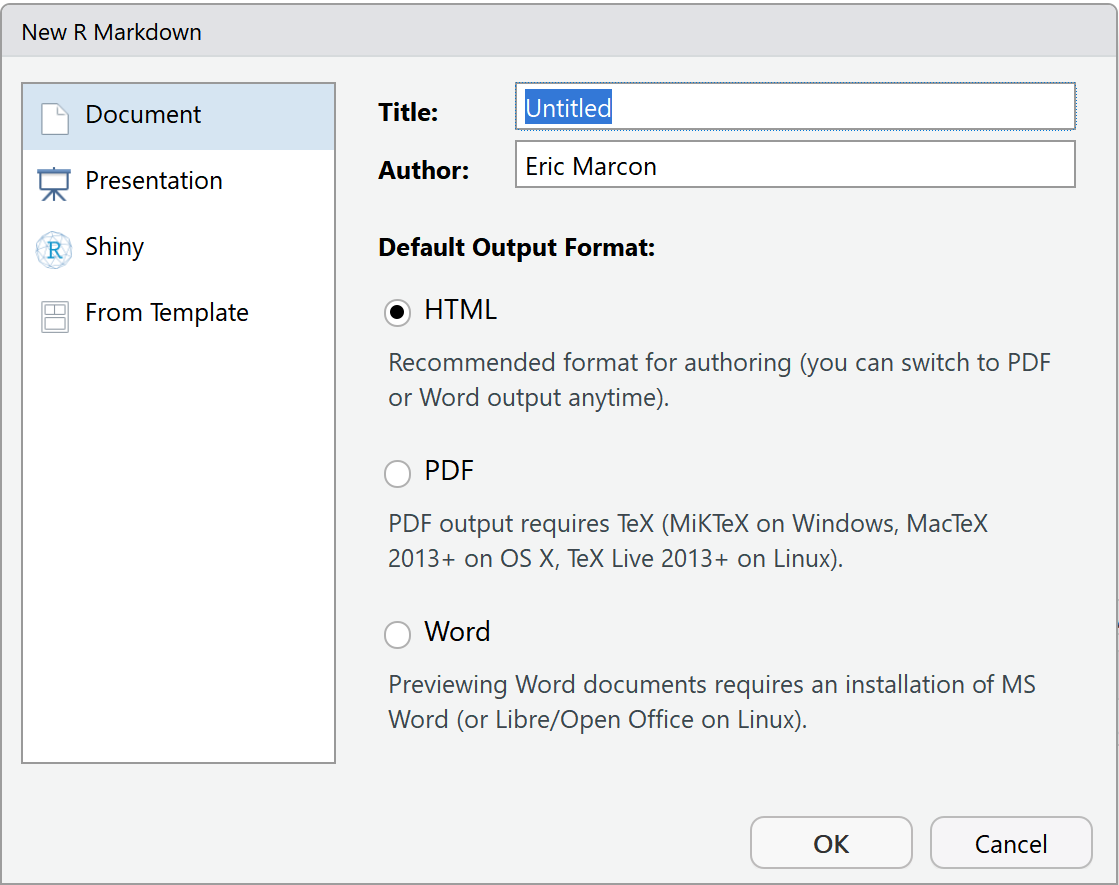
\includegraphics[width=0.8\linewidth]{images/e-rmd1} 

}

\caption{New Markdown document from a template.}\label{fig:e-rmd1}
\end{figure}

\normalsize

The simplest templates are \emph{Document} and \emph{Presentation}.
The information to be provided is the title and the name of the author, and the format of the expected document (which can be modified later).
These templates create a single file which will only need to be saved when knitting.

The syntax is the same as for the notepad.
In the header, an extra entry is used for the date, which can be calculated by R at each knitting:

\begin{verbatim}
date: "|r format(Sys.Date(), '%d/%m/%Y')|"
\end{verbatim}

Replace the vertical bars \texttt{\textbar{}} in the above example with backquotes: since this document is written with R Markdown, the date would be calculated and displayed instead of the code if the backquotes were used directly.

Inline R code (as opposed to code snippets) can be used anywhere in an R Markdown document, including in the header for the date display.
It starts with a backquote followed by `r' and ends with another backquote.

Documents can be knitted in HTML, PDF (via LaTeX) or Word format.
The header of the R Markdown file is rewritten when the knitting is started by the RStudio button which places the current output format on top of the list.

Presentations can be knitted in two HTML formats, ioslide\footnote{\url{https://bookdown.org/yihui/rmarkdown/ioslides-presentation.html}} or Slidy\footnote{\url{https://bookdown.org/yihui/rmarkdown/slidy-presentation.html}}, in Beamer (PDF) format\footnote{\url{https://bookdown.org/yihui/rmarkdown/beamer-presentation.html}} or in Powerpoint\footnote{\url{https://bookdown.org/yihui/rmarkdown/powerpoint-presentation.html}}.

The level 2 outline (\texttt{\#\#}) marks the change of slide.

Additional code, presented in the HTML format documentations, allows for specific functionality.

These templates are simple but not very useful: the R notepad is easier to use than the document template for minimalist documents.
More elaborate templates are available.

\section{Articles with bookdown}\label{articles-with-bookdown}

R Markdown does not allow you to write a scientific article.
Bibliography is not a problem because it is handled by pandoc for HTML or Word documents and outsourced to LaTeX for PDF documents.
Equations, figures and tables are numbered by LaTeX but not in HTML.
Cross-references (references to a figure number for example) are not supported.
Finally, figure and table captions only support plain text, without any formatting.

\textbf{bookdown} fills these gaps.
The package has been designed for writing books with several chapters but can be used for articles.

The \textbf{memoiR} package provides the templates shown here.
It must be installed.

\subsection{Writing}\label{writing}

The main features of Markdown are summarized here.
A quick and more complete training is offered by RStudio\footnote{\url{https://rmarkdown.rstudio.com/lesson-1.html}}.

The text is written without any formatting other than line breaks.
A simple line break has no effect on the document produced: it allows to separate sentences to simplify the tracking of the source code by git.

A line break marks a paragraph change.

The different levels of the plan are designated by the number of hashes at the beginning of the line: \texttt{\#} for a level-1 title, \texttt{\#\#} for a level-2 title, etc.
A space separates the hashes and the title text.

Bullet lists are marked by a dash (followed by a space) at the beginning of the line.
A double line break is required before the beginning of the list, but the elements of the list are separated by a simple line break.
Indented lists are created by inserting 4 spaces before the dash at the beginning of the line.
Last, numbered lists are created in the same way by replacing the hyphens by numbers, whose value is not important.

In the text, the italicized parts are surrounded by a star or an underscore (\texttt{*italic*}), while two stars mark the bold.

\subsubsection{R code}\label{r-code}

R code is included in code chunks that are easily created by clicking on the \enquote{Insert a new code chunk} button above the source code window in RStudio.
They start and end with three backquotes on a new line.
These code chunks can contain R code but also Python code for example: the type of code is indicated in the header on the first line, before the name of the code chunk, then a comma-separated list of options, for example:

\begin{verbatim}
```{r cars, echo=TRUE}
```
\end{verbatim}

The name and options are optional: the minimum header is \texttt{\{r\}}.

The most useful options are :

\begin{itemize}
\tightlist
\item
  \texttt{echo} to show (\texttt{=TRUE}) or hide (\texttt{=FALSE}) the code.
\item
  \texttt{message=FALSE} to hide the opening messages of some packages.
\item
  \texttt{warning=FALSE} to hide warnings.
\end{itemize}

The default options are declared in the code snippet named \enquote{Options} at the beginning of the Markdown document, in the \texttt{opts\_chunk\$set()} function.

The \texttt{include=FALSE} option removes any display related to the code snippet.
In a document such as a scientific article, which does not display its code, it should be used for all code snippets except those that produce figures.

\subsubsection{Figures}\label{figures}

\scriptsize

\begin{Shaded}
\begin{Highlighting}[]
\FunctionTok{plot}\NormalTok{(pressure)}
\end{Highlighting}
\end{Shaded}

\begin{figure}

{\centering 
\includegraphics[width=0.8\linewidth]{WwR_files/figure-latex/pressure-1} 

}

\caption{Figure caption}\label{fig:pressure}
\end{figure}

\normalsize

Figures can be created by the R code (figure \ref{fig:pressure}).
With Bookdown, a label is associated with each figure: its name is \texttt{fig:xxx} where \texttt{xxx} is the name of the R code snippet.
References are made with the command \texttt{\textbackslash{}@ref(fig:xxx)}.

The header of the code snippet of the figure \ref{fig:pressure} is:

\begin{verbatim}
```{r}
#| label: pressure
#| fig.cap: "Figure caption"
```
\end{verbatim}

It contains at least the name of the figure and its caption.
If the caption is long, the header is not very readable.
Furthermore, the caption is limited to simple text.
For more elaborate captions, it is possible to declare the caption in a separate paragraph that begins with the text \texttt{(ref:FigureName)}.
Figure \ref{fig:pressure2} benefits from an improved caption.



\scriptsize

\begin{figure}

{\centering 
\includegraphics[width=0.8\linewidth]{WwR_files/figure-latex/pressure2-1} 

}

\caption{Title with \emph{italic}, math (\(\sqrt\pi\)) and a reference to figure \ref{fig:pressure}}\label{fig:pressure2}
\end{figure}

\normalsize

The text in \texttt{fig.cap}, \enquote{Title of figure} previously, is replaced by \texttt{(ref:pressure)} \emph{within the backquotes} which are retained and the caption is entered in a paragraph starting with \texttt{(ref:pressure)} followed by a space.
Captions are limited to a single paragraph.

If a table of figures is used (option \texttt{lof:\ true} in the header), a short caption is required in addition to the full caption.
It is declared in \texttt{fig.scap}.

Figures that are not created by R but come from files are integrated in a piece of code by the \texttt{include\_graphics()} function whose argument is the file containing the image to be displayed.
Always place these files in the \texttt{images} folder for good organization.

\subsubsection{Tables}\label{tables}

The horizontal \texttt{-} and vertical \texttt{\textbar{}} separators allow to draw a table according to the Markdown syntax, but it is not the best method.

Tables can also be produced by R code.
The content of the table is in a dataframe.
The \texttt{kbl} function in the \emph{kableExtra} package prepares the table for display and passes the result to the \texttt{kable\_styling} function for final formatting.

\scriptsize

\begin{Shaded}
\begin{Highlighting}[]
\FunctionTok{library}\NormalTok{(}\StringTok{"tidyverse"}\NormalTok{)}
\NormalTok{my\_iris }\OtherTok{\textless{}{-}} \FunctionTok{head}\NormalTok{(iris)}
\FunctionTok{names}\NormalTok{(my\_iris) }\OtherTok{\textless{}{-}} \FunctionTok{c}\NormalTok{(}
  \StringTok{"Sepal length ($l\_s$)"}\NormalTok{, }
  \StringTok{"Width"}\NormalTok{, }
  \StringTok{"Petal length"}\NormalTok{, }
  \StringTok{"Width"}\NormalTok{, }
  \StringTok{"Species"}
\NormalTok{)}
\NormalTok{kableExtra}\SpecialCharTok{::}\FunctionTok{kbl}\NormalTok{(}
\NormalTok{  my\_iris, }
  \AttributeTok{caption =} \StringTok{"Table created by kable"}\NormalTok{, }
  \AttributeTok{booktabs =} \ConstantTok{TRUE}\NormalTok{, }
  \AttributeTok{escape =} \ConstantTok{FALSE}
\NormalTok{) }\SpecialCharTok{\%\textgreater{}\%}
\NormalTok{  kableExtra}\SpecialCharTok{::}\FunctionTok{kable\_styling}\NormalTok{(}
    \AttributeTok{bootstrap\_options =} \StringTok{"striped"}\NormalTok{, }
    \AttributeTok{full\_width =} \ConstantTok{FALSE}
\NormalTok{  )}
\end{Highlighting}
\end{Shaded}

\begin{table}
\centering
\caption{\label{tab:kable}Table created by kable}
\centering
\begin{tabular}[t]{rrrrl}
\toprule
Sepal length ($l_s$) & Width & Petal length & Width & Species\\
\midrule
5.1 & 3.5 & 1.4 & 0.2 & setosa\\
4.9 & 3.0 & 1.4 & 0.2 & setosa\\
4.7 & 3.2 & 1.3 & 0.2 & setosa\\
4.6 & 3.1 & 1.5 & 0.2 & setosa\\
5.0 & 3.6 & 1.4 & 0.2 & setosa\\
\addlinespace
5.4 & 3.9 & 1.7 & 0.4 & setosa\\
\bottomrule
\end{tabular}
\end{table}

\normalsize

The caption is specified by the \texttt{caption} argument and referencing is possible because the table is given a label whose name is \texttt{tab:} followed by the name of the code snippet (table \ref{tab:kable}).
As with the figures, an enhanced caption can be written in a separate paragraph.
A short caption for a possible list of tables (option \texttt{lot:\ true} in the header) is declared in the \texttt{caption.short} argument of \texttt{kbl()}.

Always use the \texttt{booktabs\ =\ TRUE} argument so that the thickness of the separator lines is optimal in LaTeX.
Since the table contains mathematics (in the name of the first column), the \texttt{escape\ =\ FALSE} option is necessary.

The \texttt{bootstrap\_options\ =\ "striped"} style option provides more readable tables in HTML.
Last, the \texttt{full\_width\ =\ FALSE} option allows to adjust the width of the table to its content instead of occupying the whole available width.

The \textbf{flextable} package allows creating more elaborate tables, as in the following example which displays the long sepals in color.

\scriptsize

\begin{Shaded}
\begin{Highlighting}[]
\FunctionTok{library}\NormalTok{(}\StringTok{"flextable"}\NormalTok{)}
\CommentTok{\# iris dataset}
\NormalTok{iris }\SpecialCharTok{\%\textgreater{}\%}
  \CommentTok{\# First lines}
  \FunctionTok{head}\NormalTok{() }\SpecialCharTok{\%\textgreater{}\%} 
  \CommentTok{\# Create a flextable object}
  \FunctionTok{flextable}\NormalTok{() }\SpecialCharTok{\%\textgreater{}\%}
  \CommentTok{\# Column titles}
  \FunctionTok{set\_header\_labels}\NormalTok{(}
    \AttributeTok{Sepal.Length =} \StringTok{"Sepal Length"}\NormalTok{,}
    \AttributeTok{Sepal.Width =} \StringTok{"Width"}\NormalTok{, }
    \AttributeTok{Petal.Length =} \StringTok{"Petal Length"}\NormalTok{,}
    \AttributeTok{Petal.Width =} \StringTok{"Width"}\NormalTok{,}
    \AttributeTok{Species =} \StringTok{"Species"}
\NormalTok{  ) }\SpecialCharTok{\%\textgreater{}\%}
  \CommentTok{\# Select long sepals (\textgreater{}5) and display them in red}
  \FunctionTok{color}\NormalTok{(}\SpecialCharTok{\textasciitilde{}}\NormalTok{Sepal.Length }\SpecialCharTok{\textgreater{}} \DecValTok{5}\NormalTok{, }\SpecialCharTok{\textasciitilde{}}\NormalTok{Sepal.Length, }\AttributeTok{color =} \StringTok{"red"}\NormalTok{)}
\end{Highlighting}
\end{Shaded}

\global\setlength{\Oldarrayrulewidth}{\arrayrulewidth}

\global\setlength{\Oldtabcolsep}{\tabcolsep}

\setlength{\tabcolsep}{2pt}

\renewcommand*{\arraystretch}{1.5}



\providecommand{\ascline}[3]{\noalign{\global\arrayrulewidth #1}\arrayrulecolor[HTML]{#2}\cline{#3}}

\begin{longtable}[c]{|p{0.75in}|p{0.75in}|p{0.75in}|p{0.75in}|p{0.75in}}



\ascline{1.5pt}{666666}{1-5}

\multicolumn{1}{>{\raggedleft}m{\dimexpr 0.75in+0\tabcolsep}}{\textcolor[HTML]{000000}{\fontsize{11}{11}\selectfont{\global\setmainfont{Helvetica}{Sepal\ Length}}}} & \multicolumn{1}{>{\raggedleft}m{\dimexpr 0.75in+0\tabcolsep}}{\textcolor[HTML]{000000}{\fontsize{11}{11}\selectfont{\global\setmainfont{Helvetica}{Width}}}} & \multicolumn{1}{>{\raggedleft}m{\dimexpr 0.75in+0\tabcolsep}}{\textcolor[HTML]{000000}{\fontsize{11}{11}\selectfont{\global\setmainfont{Helvetica}{Petal\ Length}}}} & \multicolumn{1}{>{\raggedleft}m{\dimexpr 0.75in+0\tabcolsep}}{\textcolor[HTML]{000000}{\fontsize{11}{11}\selectfont{\global\setmainfont{Helvetica}{Width}}}} & \multicolumn{1}{>{\raggedright}m{\dimexpr 0.75in+0\tabcolsep}}{\textcolor[HTML]{000000}{\fontsize{11}{11}\selectfont{\global\setmainfont{Helvetica}{Species}}}} \\

\ascline{1.5pt}{666666}{1-5}\endfirsthead 

\ascline{1.5pt}{666666}{1-5}

\multicolumn{1}{>{\raggedleft}m{\dimexpr 0.75in+0\tabcolsep}}{\textcolor[HTML]{000000}{\fontsize{11}{11}\selectfont{\global\setmainfont{Helvetica}{Sepal\ Length}}}} & \multicolumn{1}{>{\raggedleft}m{\dimexpr 0.75in+0\tabcolsep}}{\textcolor[HTML]{000000}{\fontsize{11}{11}\selectfont{\global\setmainfont{Helvetica}{Width}}}} & \multicolumn{1}{>{\raggedleft}m{\dimexpr 0.75in+0\tabcolsep}}{\textcolor[HTML]{000000}{\fontsize{11}{11}\selectfont{\global\setmainfont{Helvetica}{Petal\ Length}}}} & \multicolumn{1}{>{\raggedleft}m{\dimexpr 0.75in+0\tabcolsep}}{\textcolor[HTML]{000000}{\fontsize{11}{11}\selectfont{\global\setmainfont{Helvetica}{Width}}}} & \multicolumn{1}{>{\raggedright}m{\dimexpr 0.75in+0\tabcolsep}}{\textcolor[HTML]{000000}{\fontsize{11}{11}\selectfont{\global\setmainfont{Helvetica}{Species}}}} \\

\ascline{1.5pt}{666666}{1-5}\endhead



\multicolumn{1}{>{\raggedleft}m{\dimexpr 0.75in+0\tabcolsep}}{\textcolor[HTML]{FF0000}{\fontsize{11}{11}\selectfont{\global\setmainfont{Helvetica}{5.1}}}} & \multicolumn{1}{>{\raggedleft}m{\dimexpr 0.75in+0\tabcolsep}}{\textcolor[HTML]{000000}{\fontsize{11}{11}\selectfont{\global\setmainfont{Helvetica}{3.5}}}} & \multicolumn{1}{>{\raggedleft}m{\dimexpr 0.75in+0\tabcolsep}}{\textcolor[HTML]{000000}{\fontsize{11}{11}\selectfont{\global\setmainfont{Helvetica}{1.4}}}} & \multicolumn{1}{>{\raggedleft}m{\dimexpr 0.75in+0\tabcolsep}}{\textcolor[HTML]{000000}{\fontsize{11}{11}\selectfont{\global\setmainfont{Helvetica}{0.2}}}} & \multicolumn{1}{>{\raggedright}m{\dimexpr 0.75in+0\tabcolsep}}{\textcolor[HTML]{000000}{\fontsize{11}{11}\selectfont{\global\setmainfont{Helvetica}{setosa}}}} \\





\multicolumn{1}{>{\raggedleft}m{\dimexpr 0.75in+0\tabcolsep}}{\textcolor[HTML]{000000}{\fontsize{11}{11}\selectfont{\global\setmainfont{Helvetica}{4.9}}}} & \multicolumn{1}{>{\raggedleft}m{\dimexpr 0.75in+0\tabcolsep}}{\textcolor[HTML]{000000}{\fontsize{11}{11}\selectfont{\global\setmainfont{Helvetica}{3.0}}}} & \multicolumn{1}{>{\raggedleft}m{\dimexpr 0.75in+0\tabcolsep}}{\textcolor[HTML]{000000}{\fontsize{11}{11}\selectfont{\global\setmainfont{Helvetica}{1.4}}}} & \multicolumn{1}{>{\raggedleft}m{\dimexpr 0.75in+0\tabcolsep}}{\textcolor[HTML]{000000}{\fontsize{11}{11}\selectfont{\global\setmainfont{Helvetica}{0.2}}}} & \multicolumn{1}{>{\raggedright}m{\dimexpr 0.75in+0\tabcolsep}}{\textcolor[HTML]{000000}{\fontsize{11}{11}\selectfont{\global\setmainfont{Helvetica}{setosa}}}} \\





\multicolumn{1}{>{\raggedleft}m{\dimexpr 0.75in+0\tabcolsep}}{\textcolor[HTML]{000000}{\fontsize{11}{11}\selectfont{\global\setmainfont{Helvetica}{4.7}}}} & \multicolumn{1}{>{\raggedleft}m{\dimexpr 0.75in+0\tabcolsep}}{\textcolor[HTML]{000000}{\fontsize{11}{11}\selectfont{\global\setmainfont{Helvetica}{3.2}}}} & \multicolumn{1}{>{\raggedleft}m{\dimexpr 0.75in+0\tabcolsep}}{\textcolor[HTML]{000000}{\fontsize{11}{11}\selectfont{\global\setmainfont{Helvetica}{1.3}}}} & \multicolumn{1}{>{\raggedleft}m{\dimexpr 0.75in+0\tabcolsep}}{\textcolor[HTML]{000000}{\fontsize{11}{11}\selectfont{\global\setmainfont{Helvetica}{0.2}}}} & \multicolumn{1}{>{\raggedright}m{\dimexpr 0.75in+0\tabcolsep}}{\textcolor[HTML]{000000}{\fontsize{11}{11}\selectfont{\global\setmainfont{Helvetica}{setosa}}}} \\





\multicolumn{1}{>{\raggedleft}m{\dimexpr 0.75in+0\tabcolsep}}{\textcolor[HTML]{000000}{\fontsize{11}{11}\selectfont{\global\setmainfont{Helvetica}{4.6}}}} & \multicolumn{1}{>{\raggedleft}m{\dimexpr 0.75in+0\tabcolsep}}{\textcolor[HTML]{000000}{\fontsize{11}{11}\selectfont{\global\setmainfont{Helvetica}{3.1}}}} & \multicolumn{1}{>{\raggedleft}m{\dimexpr 0.75in+0\tabcolsep}}{\textcolor[HTML]{000000}{\fontsize{11}{11}\selectfont{\global\setmainfont{Helvetica}{1.5}}}} & \multicolumn{1}{>{\raggedleft}m{\dimexpr 0.75in+0\tabcolsep}}{\textcolor[HTML]{000000}{\fontsize{11}{11}\selectfont{\global\setmainfont{Helvetica}{0.2}}}} & \multicolumn{1}{>{\raggedright}m{\dimexpr 0.75in+0\tabcolsep}}{\textcolor[HTML]{000000}{\fontsize{11}{11}\selectfont{\global\setmainfont{Helvetica}{setosa}}}} \\





\multicolumn{1}{>{\raggedleft}m{\dimexpr 0.75in+0\tabcolsep}}{\textcolor[HTML]{000000}{\fontsize{11}{11}\selectfont{\global\setmainfont{Helvetica}{5.0}}}} & \multicolumn{1}{>{\raggedleft}m{\dimexpr 0.75in+0\tabcolsep}}{\textcolor[HTML]{000000}{\fontsize{11}{11}\selectfont{\global\setmainfont{Helvetica}{3.6}}}} & \multicolumn{1}{>{\raggedleft}m{\dimexpr 0.75in+0\tabcolsep}}{\textcolor[HTML]{000000}{\fontsize{11}{11}\selectfont{\global\setmainfont{Helvetica}{1.4}}}} & \multicolumn{1}{>{\raggedleft}m{\dimexpr 0.75in+0\tabcolsep}}{\textcolor[HTML]{000000}{\fontsize{11}{11}\selectfont{\global\setmainfont{Helvetica}{0.2}}}} & \multicolumn{1}{>{\raggedright}m{\dimexpr 0.75in+0\tabcolsep}}{\textcolor[HTML]{000000}{\fontsize{11}{11}\selectfont{\global\setmainfont{Helvetica}{setosa}}}} \\





\multicolumn{1}{>{\raggedleft}m{\dimexpr 0.75in+0\tabcolsep}}{\textcolor[HTML]{FF0000}{\fontsize{11}{11}\selectfont{\global\setmainfont{Helvetica}{5.4}}}} & \multicolumn{1}{>{\raggedleft}m{\dimexpr 0.75in+0\tabcolsep}}{\textcolor[HTML]{000000}{\fontsize{11}{11}\selectfont{\global\setmainfont{Helvetica}{3.9}}}} & \multicolumn{1}{>{\raggedleft}m{\dimexpr 0.75in+0\tabcolsep}}{\textcolor[HTML]{000000}{\fontsize{11}{11}\selectfont{\global\setmainfont{Helvetica}{1.7}}}} & \multicolumn{1}{>{\raggedleft}m{\dimexpr 0.75in+0\tabcolsep}}{\textcolor[HTML]{000000}{\fontsize{11}{11}\selectfont{\global\setmainfont{Helvetica}{0.4}}}} & \multicolumn{1}{>{\raggedright}m{\dimexpr 0.75in+0\tabcolsep}}{\textcolor[HTML]{000000}{\fontsize{11}{11}\selectfont{\global\setmainfont{Helvetica}{setosa}}}} \\

\ascline{1.5pt}{666666}{1-5}



\end{longtable}



\arrayrulecolor[HTML]{000000}

\global\setlength{\arrayrulewidth}{\Oldarrayrulewidth}

\global\setlength{\tabcolsep}{\Oldtabcolsep}

\renewcommand*{\arraystretch}{1}

\normalsize

The package documentation\footnote{\url{https://ardata-fr.github.io/flextable-book/}} is available online, as well as a gallery\footnote{\url{https://ardata-fr.github.io/flextable-gallery/gallery/}}.

\textbf{flextable} does not support caption numbering except in Word documents.
This limitation is prohibitive.

\subsubsection{Maths}\label{maths}

Equations in LaTeX format can be inserted inline, like \(A=\pi r^2\) (code: \texttt{\$A=\textbackslash{}pi\ r\^{}2\$}) or in a new line (the \$ are doubled) like \[e^{i \pi} = -1.\]

They can be numbered: see equation \eqref{eq:disc}, using the \texttt{\textbackslash{}equation} environment.

\begin{equation}
  A = \pi r^2.
  \label{eq:disc}
\end{equation}

The numbered equation is created by the following code:

\begin{verbatim}
\begin{equation}
  A = \pi r^2.
  \label{eq:disc}
\end{equation}
\end{verbatim}

\subsubsection{Cross-references}\label{cross-references}

Figures and tables have an automatically generated label, identical to the name of the code snippet prefixed with \texttt{fig:} and \texttt{tab:}.

For equations, the label is added manually by the code \texttt{(\textbackslash{}\#eq:xxx)} before the end of the equation.

Sections can be given a label by completing their title with \texttt{\{\#yyy\}}.
Sections receive by default an implicit label\footnote{\url{https://pandoc.org/MANUAL.html\#extension-implicit_header_references}} corresponding to their text, in lower case, where special characters are replaced by dashes.
Implicit labels are unstable (they change with the title of the section) and difficult to predict: this is why it is advisable to add an explicit label to each section being cross-referenced.
This is the case for chapters, for which the name of the HMTL file produced is identical to the label.
Chapter labels must follow file naming rules by not containing special characters.

Bookmarks can also be placed freely in the text with the command \texttt{(ref:zzz)}.

In all cases, the call to the reference is made by the command \texttt{\textbackslash{}@ref(ref:zzz)}.

\subsubsection{Bibliography}\label{bibliography}

Bibliographic references in BibTeX format must be included in the \texttt{.bib} file declared in the header of the Markdown document.

\begin{verbatim}
bibliography: references.bib
\end{verbatim}

This file can be created and maintained by Zotero installed with the Better BibTeX extension (see section \ref{sec:Zotero}).
To do this, you just have to create a Zotero collection corresponding to the project and drag the relevant references into it.
Then use the contextual menu \enquote{Export collection\ldots{}} and select:

\begin{itemize}
\tightlist
\item
  Format: \enquote{Better BibTeX} for articles and presentations or \enquote{Better BibLaTeX} for memoirs, depending on whether the bibliography is managed by BibTeX and natbib or biber and BibLaTeX for PDF production.
\item
  Check the \enquote{Keep up to date} box so that any changes in Zotero are exported automatically.
\item
  Click on \enquote{OK} then choose the name of the file (\texttt{references.bib}) and its location (the R project folder).
\end{itemize}

The references can be called in the text, between square brackets by the code \texttt{{[}@Reference{]}}, or in the text, by removing the brackets.

The bibliography is handled by pandoc when producing Word or HTML documents.
The bibliographic style can be specified, by adding the line

\begin{verbatim}
csl:nom_du_fichier.csl
\end{verbatim}

in the document header and copying the \emph{.csl} style file to the project folder.
Over a thousand styles are available\footnote{\url{https://github.com/citation-style-language/styles}}.

For PDF documents, the bibliography is managed by LaTeX.

To prepare the submission of a manuscript to a journal, it will be necessary to open the intermediate \emph{.tex} file produced by pandoc and copy the contents of the environment \{document\} into the template proposed by the journal, which will take care of the formatting.

\subsubsection{Languages}\label{languages}

The languages are to be declared in the header of the documents produced by the \textbf{memoiR} templates.

The main language of the document modifies the name of certain elements, such as the table of contents.
The additional languages allow the creation of multilingual documents.

The header fields are:

\begin{verbatim}
lang: fr-FR
otherlangs: [en-US, it]
\end{verbatim}

The change of language in the document is managed in LaTeX, but not in HTML, by inserting on a new line the following command:

\begin{verbatim}
\selectlanguage{english}
\end{verbatim}

The current language only has an effect in LaTeX output: a space is added before double punctuation in French, the size of spaces is larger at the beginning of sentences in English, etc.
The \texttt{\textbackslash{}selectlanguage} command is simply ignored in HTML.

The language names are different in the header (IETF codes) and in the text (language name).
The correspondence and the complete list of languages can be found in table 3 of the package documentation \textbf{polyglossia}\footnote{\url{http://mirrors.ctan.org/macros/unicodetex/latex/polyglossia/polyglossia.pdf}}.

HTML formatting of punctuation in French documents is possible using a filter declared in pandoc \footnote{\url{https://github.com/InseeFrLab/pandoc-filter-fr-nbsp}}.
The \texttt{fr-nbsp.lua} file must be copied into the project directory from its GitHub repository and declared into the header of the Markdown document.

\begin{verbatim}
output:
    pandoc_args:
      --lua-filter=en-nbsp.lua
\end{verbatim}

The filter formats all the punctuation in the document, whatever the language: it should therefore only be used for documents written entirely in French.

\subsection{Simple Article template}\label{sec:memo}

The \emph{Simple Article} template of \textbf{memoiR} produces a simple HTML document with a floating table of contents (see example\footnote{\url{https://EricMarcon.github.io/Krigeage/Krigeage.html}}).
Other HTML formats are available: see the gallery\footnote{\url{https://ericmarcon.github.io/memoiR/}} of the package.
The PDF format is close to the \emph{article} model of LaTeX (example\footnote{\url{https://EricMarcon.github.io/Krigeage/Krigeage.pdf}}).

The template contains its own documentation.

\subsubsection{Create}\label{create}

Use the menu \enquote{File \textgreater{} New File \textgreater{} R Markdown\ldots{}} then select \enquote{From template} (figure \ref{fig:e-rmd1}).
The list of available templates and the package that offers them is then displayed.

Select the \emph{Simple Article} template from the \textbf{memoiR} package, choose the name of the project (\enquote{Name:}, which will be the name of the folder in which it will be created, and its parent folder (\enquote{Location:}).
In the organization proposed in section \ref{sec:solution-dossiers}, the parent folder is \texttt{\%LOCALAPPDATA\%\textbackslash{}ProjectsR}.
The project name must not contain any special characters (accent, space\ldots) to ensure its portability on all operating systems (Windows, Linux, MacOS).

Advanced templates create a folder with many files (bibliography, styles, LaTeX template\ldots), unlike simple templates which create only one file.

When a folder is created, for example by the \emph{Simple Article} template, you have to make it an RStudio project: in the projects menu (top right of the RStudio window), use the \enquote{New Project\ldots{}} menu, then \enquote{Existing Directory} and select the folder that has just been created.

\subsubsection{Write}\label{write}

The instructions for using the template are contained in the text provided by default.

\subsubsection{Knit}\label{knit}

The document can be knitted in several formats:

\begin{itemize}
\tightlist
\item
  \emph{html\_document2} is the HTML format the template was designed for: a notepad with a floating table of contents.
\item
  \emph{gitbook} is an alternative HTML format, normally used for books.
\item
  \emph{downcute} is an HTML format provided by the \textbf{rmdformats} package.
\item
  \emph{pdf\_book} produces a PDF document following the LaTeX \emph{article} template, commonly used directly in LaTeX.
\item
  \emph{word\_document2} creates a Word file.
\end{itemize}

\subsubsection{Publish}\label{sec:article-en-ligne}

The \textbf{memoiR} package simplifies the uploading of produced documents to a web server.

The \texttt{build\_gitignore()} function creates a \texttt{.gitignore} file for source control which must be enabled (see section \ref{sec:git-cds}).

The \texttt{build\_readme()} function creates a \texttt{README.md} file that is needed by GitHub.
It contains the title of the project, its summary and links to the HTML and PDF versions of the documents produced.

The project must be linked to a GitHub repository (section \ref{sec:creerdepot}).

Two publication strategies are possible.
In the first one, the documents are knitted locally and placed in the \texttt{docs} folder, which will be the support of the GitHub pages.
In the second one, the documents are knitted by GitHub Actions each time modifications are pushed on the repository: this is called continuous integration (section \ref{chap-ci}).

The local production strategy is covered here; continuous integration will be covered in section \ref{sec:memoiR-ci}.

The \texttt{build\_githubpages()} function places all the knitted documents (HTML and PDF) in the \texttt{docs} folder, along with a copy of the \texttt{README.md} file.
This way, it is possible to activate the project's GitHub pages (on the \texttt{docs} folder of the \texttt{master} branch).
The \texttt{README.md} file will be the home page of the produced web site.

In practice, we knit in HTML format during the whole writing phase, because the production is very fast.
When the document is stabilized, it should be knitted in HTML and PDF format.
Finally, the execution of \texttt{build\_githubpages()} places all the files produced in \texttt{docs}.
It remains to push the repository on GitHub and activate the GitHub pages.

\subsection{Other templates}\label{other-templates}

The \emph{Stylish Article} template of \textbf{memoiR} is intended for the production of well-formatted PDF articles for self-archiving (typically, the HAL repository), in A4 format in double column\footnote{Exemple: \url{https://EricMarcon.github.io/Rochebrune2018/Entropie.pdf}}.

The HTML format is the same as the \emph{Simple Article} template.

The \textbf{rticles} package aims to provide templates for all scientific journals that accept article submission in LaTeX.
It offers Markdown templates which produce PDF files conforming to the requirements of the journals and the possibility to recover the intermediate \texttt{.tex} file (pandoc produces a \texttt{.tex} file transmitted to the LaTeX compiler).
The package does not allow HTML knitting because it uses LaTeX syntax in the R Markdown document instead of using \textbf{bookdown} to handle bibliographic and cross references.
It is not possible to directly exchange standard R Markdown content with documents written for \textbf{rticles}, which limits the interest of the package.

\section{Beamer Presentation}\label{beamer-presentation}

The \emph{Beamer Presentation} template of \textbf{memoiR} allows to create HTML and PDF (beamer) presentations simultaneously, as shown in the example\footnote{\url{https://EricMarcon.github.io/Chao1/}, Choose \enquote{Lecture} (Read in HTML) ou \enquote{Téléchargement} (Download PDF).}.

The approach is identical to that of articles in the same package.
The title levels allow separating the parts of the presentation (\texttt{\#}) and the slides (\texttt{\#\#}).
Two formats are available in HTML: ioslides\footnote{\url{https://bookdown.org/yihui/rmarkdown/ioslides-presentation.html}} and Slidy\footnote{\url{https://bookdown.org/yihui/rmarkdown/slidy-presentation.html}}.
Some specificities in the code allow to refine the presentation of the slides, for a two-column display for example: they are documented in the template.

\section{memoir}\label{memoir}

The \emph{Memoir} template of the \textbf{memoiR} package is intended for long documents, which have an important difference from the previous documents: a long document is composed of several chapters, each placed in its \texttt{.Rmd} file.

The HTML format is gitbook\footnote{\url{https://www.gitbook.com/}}, the standard for reading such documents online.
The PDF format is derived from the LaTeX \emph{memoir}\footnote{\url{https://www.ctan.org/pkg/memoir}} template, also optimized for long documents.

This document was written with this template.

\subsection{Create}\label{create-1}

Creating a work project is identical to the one presented above: the template is: \emph{Memoir}.
The created folder must be turned into a project.

Run \texttt{build\_git()} and \texttt{build\_readme()}, enable source control and push the project to GitHub, in the same way as for an article (section \ref{sec:article-en-ligne}).

Each chapter of the book is an Rmd file, whose name normally starts with its number (e.g.: \texttt{01-intro.Rmd}).
All Rmd files in the project folder are actually treated as chapters, sorted by filename, including those provided by the template (startup and syntax) which should be deleted except for \texttt{99-references.Rmd} which contains the bibliography, placed at the end.
The \texttt{index.Rmd} file is special: it contains the document header and the first chapter.

\subsection{Write}\label{write-1}

The first chapter is placed in the front matter of the printed book: it should not be numbered (hence the \texttt{\{-\}} code next to the title) in the HTML version.
It must end with the LaTeX command \texttt{\textbackslash{}mainmatter} which marks the beginning of the body of the book.

The outline levels start with \texttt{\#} for chapters (only one per file), \texttt{\#\#} for sections, etc.

\subsection{Knit}\label{knit-1}

Compiling to PDF is done by XeLaTeX, which must be installed.

While writing, it is strongly advised to create only the HTML file, which is much faster than a LaTeX compilation.
Each chapter can be viewed very quickly by clicking on the \enquote{Knit} button above the source window.
The entire book is created by clicking on the \enquote{Build Book} button in the RStudio \emph{Build} window.
The button's drop-down list allows you to create all documents or limit yourself to one format.

The files produced are placed directly in the \texttt{docs} folder, which will be used by the GitHub pages to allow online reading and downloading of the PDF.
The home page of the website is created by bookdown from the \texttt{index.Rmd} file: the \texttt{README.md} file is not duplicated in \texttt{docs}.

\subsection{Finishing}\label{finishing}

The layout is done fully automatically by pandoc (in HTML) and LaTeX (in PDF).

It is often useful to help LaTeX to solve some margin overruns due to too large layout constraints: for optimal readability, columns are narrow, but code (formatted text between backquotes) does not allow hyphenation.

If a line of text protrudes into the right margin in the PDF document, the solution is to manually add the \texttt{\textbackslash{}break} code to the desired location for the line break in the R Markdown document.
The command has no effect on the HTML document but forces the hyphenation in LaTeX.
To break formatted text (between asterisks for italics or more frequently between backquotes for code), you must finish formatting before \texttt{\textbackslash{}break} and start again afterwards.
For example, to force a line break before \texttt{file.Rmd}:

\begin{verbatim}
The file `/path/`\break`file.Rmd`
\end{verbatim}

In HTML, a space will be added between the two pieces of code.

R code snippets are automatically formatted by \textbf{knitr} when the \texttt{tidy=TRUE} option is applied to them.
The default behavior is specified in the \textbf{knitr} options, in a code snippet at the beginning of the \texttt{index.Rmd} file:

\scriptsize

\begin{Shaded}
\begin{Highlighting}[]
\CommentTok{\# knitr options}
\NormalTok{knitr}\SpecialCharTok{::}\NormalTok{opts\_chunk}\SpecialCharTok{$}\FunctionTok{set}\NormalTok{(}
  \AttributeTok{cache =} \ConstantTok{TRUE}\NormalTok{, }\AttributeTok{warning =} \ConstantTok{FALSE}\NormalTok{, }\AttributeTok{echo =} \ConstantTok{TRUE}\NormalTok{,}
  \AttributeTok{fig.env =} \StringTok{\textquotesingle{}SCfigure\textquotesingle{}}\NormalTok{, }\AttributeTok{fig.asp =}\NormalTok{ .}\DecValTok{75}\NormalTok{, }
  \AttributeTok{fig.align =} \StringTok{\textquotesingle{}center\textquotesingle{}}\NormalTok{, }\AttributeTok{out.width =} \StringTok{\textquotesingle{}80\%\textquotesingle{}}\NormalTok{, }
  \AttributeTok{tidy =} \ConstantTok{TRUE}\NormalTok{, }
  \AttributeTok{tidy.opts =} \FunctionTok{list}\NormalTok{(}\AttributeTok{blank =} \ConstantTok{FALSE}\NormalTok{, }\AttributeTok{width.cutoff =} \DecValTok{55}\NormalTok{), }
  \AttributeTok{size =} \StringTok{"scriptsize"}\NormalTok{, }
  \AttributeTok{knitr.graphics.auto\_pdf =} \ConstantTok{TRUE}
\NormalTok{)}
\end{Highlighting}
\end{Shaded}

\normalsize

The maximum width of a line of formatted code here is 55 characters, optimal for the template.
Sometimes automatic formatting does not work because \textbf{knitr} cannot find a line break that meets all the constraints, causing the code to overflow.
In this case, manually format the code snippet by adding the \texttt{tidy=FALSE} option.

The literal code blocks, delimited by three backquotes, must be formatted manually, avoiding any line longer than 55 characters.

\subsection{Gitbook site}\label{gitbook-site}

The website containing the gitbook document must be set up in \texttt{\_output.yml} so that :

\begin{itemize}
\tightlist
\item
  The title of the document appears at the top of the table of contents.
\item
  An indication of the use of GitHub and bookdown is displayed at the bottom of the table of contents.
\item
  A GitHub button in the title bar allows to open the project repository.
\item
  Another button allows to download the PDF document.
\end{itemize}

The \texttt{\_output.yml} file of this document is the following:

\begin{verbatim}
bookdown::gitbook:
  css: style.css
  config:
    sharing:
      github: yes
      facebook: false
      twitter: false
    toc:
      before: |
        <li><a href="./">Working with R</a></li>
      after: |
        <li>
          <a href="https://github.com/EricMarcon/WorkingWithR" target="blank">
            Hosted on GitHub, published by bookdown
          </a>
        </li>
    download: pdf
\end{verbatim}

The \texttt{sharing:} section manages the buttons in the title bar.
By default, the links to Facebook and Twitter are enabled but the one to GitHub is not.
For it to work, the GitHub repository must be declared in the header of the \texttt{index.rmd} file:

\begin{verbatim}
github-repo: EricMarcon/WorkingWithR
\end{verbatim}

The \texttt{toc:} section contains two portions of HTML code in which the title of the document and the link to its GitHub repository must be adapted to the project.

Finally, the \texttt{download:} section lists the downloadable document formats and displays a download button in the title bar.

\subsection{Continuous integration}\label{sec:rediger-ouvrage-ci}

Building a book takes time, especially if it contains calculations.
It must be launched in gitbook format and in PDF format.
In production, it can be outsourced to GitHub (chapter \ref{sec:bookdown-ci}).

\subsection{Google Analytics}\label{google-analytics}

The tracking of the book's audience can be entrusted to Google Analytics.
To do so, you have to create an account and add a Google Analytics \emph{property}, i.e.~a website, then a data feed, here a web feed\footnote{\url{https://support.google.com/analytics/answer/9304153?hl=fr&ref_topic=9303319}}.

Google Analytics provides a configuration script named \texttt{gtag.js} to be placed at the root of the project folder.
Finally, declare the script in the header of the web pages by adding a statement in \texttt{\_output.yml}, in its first section.

\begin{verbatim}
bookdown::gitbook:
  includes:
    in_header: gtag.js
\end{verbatim}

\section{R Markdown web site}\label{r-markdown-web-site}

A web site made of pages written with R Markdown (without the \textbf{bookdown} features) and a menu can be created very easily, with a good result\footnote{\url{https://rstudio.github.io/learnr/} for example.}.

\subsection{Template}\label{template}

In RStudio, in the projects menu at the top right, click on \enquote{New Project\ldots{}} then \enquote{New Directory} then \enquote{Simple R Markdown website}.
Enter the name of the project, select the folder in which the project will be created by clicking on \enquote{Browse} and finally click on \enquote{Create Project}.

The default site contains two pages: \texttt{index}, the home page, and \texttt{about}, the \enquote{About} page.
The \texttt{\_site.yml} file contains the name of the site and the contents of its navigation bar: a title and the corresponding file.
Other pages will be added by creating new \texttt{.Rmd} files and adding them to the \texttt{\_site.yml} file.

\subsection{Improvements}\label{improvements}

The site template can easily be enhanced by adding lines to \texttt{\_site.yml}:

\begin{itemize}
\tightlist
\item
  To add a GitHub icon in the navigation bar to link to the site source code.
\item
  To choose the method of knitting, to use \textbf{bookdown} instead of \textbf{rmarkdown}.
\item
  To place the site files in the \texttt{docs} folder and thus separate code and production.
\end{itemize}

The completed \texttt{\_site.yml} file is as follows:

\begin{verbatim}
name: "my-website"
navbar:
  title: "My Website"
  left:
    - text: "Home"
      href: index.html
    - text: "About"
      href: about.html
  right:
    - icon: fa-github
      href: https://github.com/rstudio/rmarkdown
output_dir: "docs"
output:
  bookdown::html_document2:
    theme: sandstone
    highlight: tango
    toc: true
    toc_float: yes
\end{verbatim}

The GitHub icon is part of the Font Awesome collection of which all free icons\footnote{\url{https://fontawesome.com/icons?d=gallery&m=free}} are usable with the same syntax: \enquote{fa-name}.

The link corresponding to the icon must be the one in the website's GitHub repository.

The syntax of the \texttt{output} section is the same as that of the documents seen above.
It applies to all pages (with the YAML header reduced to the minimum).
The available themes are those of rmarkdown\footnote{\url{https://bookdown.org/yihui/rmarkdown/html-document.html\#appearance-and-style}}.

The \texttt{highlight} option specifies how any R code displayed will be formatted.
Last, the table of contents is floating, which means that its position adjusts as the window scrolls.

\subsection{Source control}\label{source-control}

The project must be put under source control and pushed to GitHub (chapter \ref{chap-git}).
The \texttt{.gitignore} file is the following:

\begin{verbatim}
# R
.Rbuildignore
.RData
.Rhistory
.Rprofile
.Rproj.user

# Web Site
/_site/
/*_cache/
/*_files/
\end{verbatim}

Enable GitHub pages (section \ref{sec:github-pages}) on the \texttt{docs} folder to host the site.
Add an empty file named \texttt{.nojekyll} in \texttt{docs} so that GitHub pages won't try to reformat the site.
You can use the RStudio terminal to run:

\begin{verbatim}
touch docs/.nojekyll
\end{verbatim}

\section{Personal web site: blogdown}\label{sec:blogdown}

To create a personal web page, \emph{Hugo} is a static site generator capable of producing HTML pages from Markdown code.
Static sites have the advantage, compared to dynamic sites managed by a content management system (CMS, for example: Wordpress, Joomla, SPIP), to be portable on any web server without database support or code to run on the server side (such as PHP) and to be very fast since the pages are created once and not at each consultation.
A Hugo site can be hosted for example on the personal page of any GitHub user.
Its address is of the form \enquote{GitHubID.github.io}.

Hugo offers many themes, which are templates for site structure, so the \textbf{Academic} theme, intended for researchers.
In RStudio, the \textbf{blogdown} package is provided to easily produce web pages with Hugo.
These pages can contain R code: they are very similar to an article, seen above, whose content can be easily copied and pasted.
So we will use this solution, for a site like the one proposed in example\footnote{\url{https://EricMarcon.github.io/}}.

The structure of the website is simple:

\begin{itemize}
\tightlist
\item
  A home page, containing various customizable components such as the author's biography, a selection of publications, blog posts or other elements and a contact form.
\item
  Pages detailing the various elements (publications, posts, etc.) written in R Markdown.
\end{itemize}

\subsection{Installing the tools}\label{installing-the-tools}

The first step is to install the \textbf{blogdown} package in R.

\scriptsize

\begin{Shaded}
\begin{Highlighting}[]
\FunctionTok{install.packages}\NormalTok{(}\StringTok{\textquotesingle{}blogdown\textquotesingle{}}\NormalTok{) }
\end{Highlighting}
\end{Shaded}

\normalsize

\textbf{blogdown} is able to install Hugo on Windows, macOS or Linux.

\scriptsize

\begin{Shaded}
\begin{Highlighting}[]
\NormalTok{blogdown}\SpecialCharTok{::}\FunctionTok{install\_hugo}\NormalTok{()}
\end{Highlighting}
\end{Shaded}

\normalsize

The full documentation for \textbf{blogdown} is available\footnote{\url{https://bookdown.org/yihui/blogdown/}}.

Recent versions of Hugo use \emph{Go} (the programming language) to install their modules on the fly: here the Academic theme is loaded from GitHub at the time of site creation.
Go must therefore be installed\footnote{\url{https://golang.org/doc/install}}.

\subsection{Create}\label{create-2}

The easiest way is to create a repository on GitHub from the template.
On the \emph{starter-academic}\footnote{\url{https://github.com/wowchemy/starter-academic}} repository page, click on the \enquote{Use this template} button, optionally authenticate to GitHub, and then enter the name of the repository that will contain the project, for example \enquote{MySite}.

The repository can be the one of the main site of your GitHub account (see section \ref{sec:github-pages}), at the address \url{https://GitHubID.github.io}\footnote{Exemple: \url{https://EricMarcon.github.io/Krigeage/}}.
The name to enter is simply \enquote{GitHubID.github.io} (\emph{GitHubID} is the name of the GitHub account).

Create the repository.
Copy the repository address by clicking on the \enquote{Code} button and then on the button to the right of the address (figure \ref{fig:rediger-GitHub-Clone}).



\scriptsize

\begin{figure}

{\centering 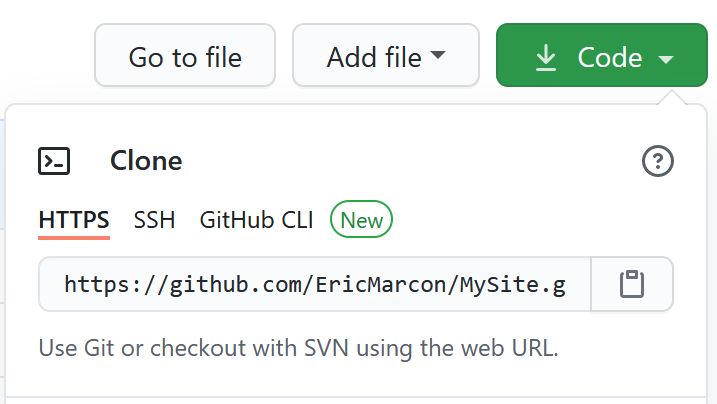
\includegraphics[width=0.8\linewidth]{images/rediger-GitHub-Clone} 

}

\caption{Copy of the address of a repository to clone on GitHub.}\label{fig:rediger-GitHub-Clone}
\end{figure}

\normalsize

In RStudio, create a new project from GitHub: in the projects menu on the top right, click on \enquote{New Project\ldots{}} then \enquote{Version Control} then \enquote{Git} then paste the address in the \enquote{Repository URL} field (figure \ref{fig:rediger-Projet-GitHub}).
Select the folder in which the project will be created by clicking on \enquote{Browse} and finally click on \enquote{Create Project}.



\scriptsize

\begin{figure}

{\centering 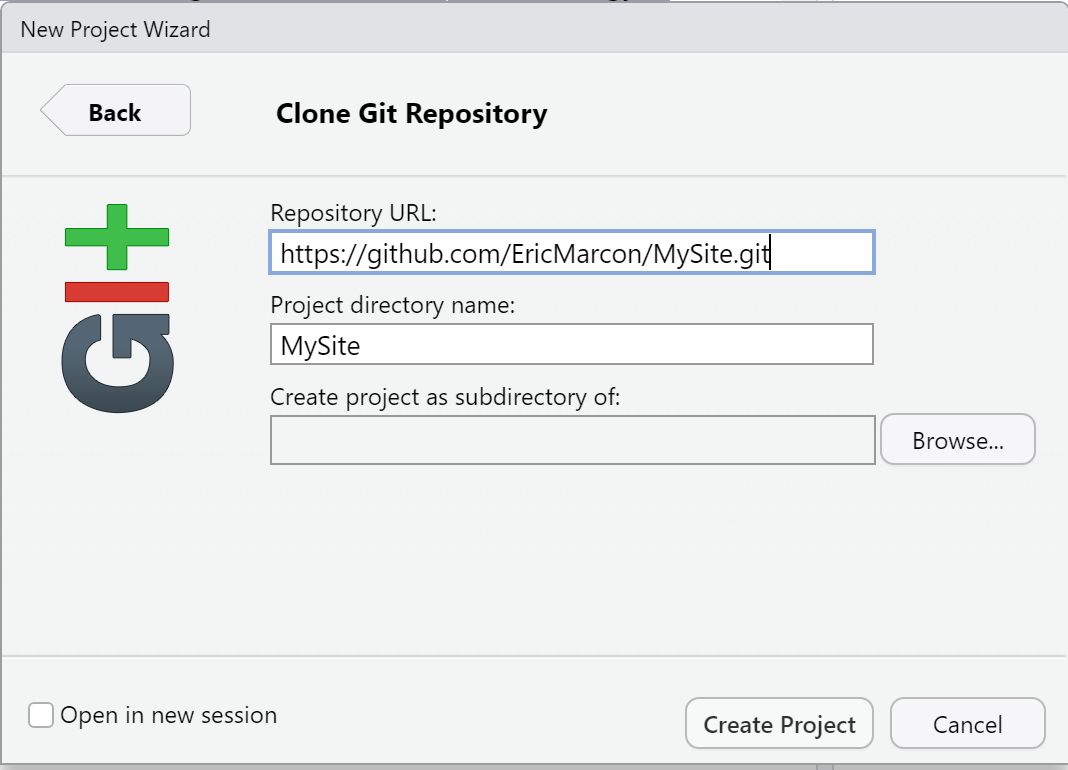
\includegraphics[width=0.8\linewidth]{images/rediger-Projet-GitHub} 

}

\caption{Copy the address of a repository to clone to GitHub.}\label{fig:rediger-Projet-GitHub}
\end{figure}

\normalsize

The created project is an exact copy of the template, which must be customized.

RStudio automatically adds a line at the end of the \texttt{.gitignore} file to ignore its working files (\texttt{.Rproj.user} folder).
Add a comment line to indicate this.
The content of \texttt{.gitignore} should be as follows:

\begin{verbatim}
# R
.Rbuildignore
.RData
.Rhistory
.Rprofile
.Rproj.user

# Hugo
/resources/
/public/

# blogdown
/static/en/
/static/fr/
*.rmarkdown
_index.html
index.html
**/index_files/
\end{verbatim}

A bug of \textbf{blogdown} requires to move the file \texttt{config.toml} from the folder \texttt{config/\_default/} to the root of the project.

Take into account these modifications in git by making a commit.

\subsection{Building the site}\label{building-the-site}

Run

\scriptsize

\begin{Shaded}
\begin{Highlighting}[]
\NormalTok{blogdown}\SpecialCharTok{::}\FunctionTok{build\_site}\NormalTok{(}\AttributeTok{build\_rmd =} \ConstantTok{TRUE}\NormalTok{)}
\end{Highlighting}
\end{Shaded}

\normalsize

to build the website, including its future R Markdown pages.

To display the site, run:

\scriptsize

\begin{Shaded}
\begin{Highlighting}[]
\NormalTok{blogdown}\SpecialCharTok{:::}\FunctionTok{serve\_site}\NormalTok{()}
\end{Highlighting}
\end{Shaded}

\normalsize

It appears in the RStudio \emph{Viewer} window, which can be viewed in the system's default web browser by clicking the enlarge button.

To modify the content of the site, it is best to stop the web server with the command:

\scriptsize

\begin{Shaded}
\begin{Highlighting}[]
\NormalTok{blogdown}\SpecialCharTok{:::}\FunctionTok{stop\_server}\NormalTok{()}
\end{Highlighting}
\end{Shaded}

\normalsize

The site produced by \textbf{blogdown} is located in the \texttt{public} folder which can be copied directly to a web server that will host it.
A simple solution is to declare this folder as the root of the GitHub pages of the project
(section \ref{sec:github-pages}).
The optimal method is to use continuous integration (see section \ref{sec:blogdown-ci}) to copy it to the root of the \texttt{gh-pages} branch which will be declared as the location of the site on GitHub.

\subsection{Multilingual site}\label{multilingual-site}

If the site is multilingual (say English and French), its \texttt{content} folder must be copied in a folder corresponding to each language.
The files in \texttt{content/authors/admin/} must be duplicated into \texttt{content/en/authors}\break\texttt{/admin/} and \texttt{content/fr/authors/admin/}.
In practice, create an \texttt{en} folder and an \texttt{fr} folder in \texttt{content}.
Move all the original \texttt{content} folder \texttt{en} and then copy it into \texttt{fr}.

\subsection{Set up}\label{set-up}

The site configuration files are well documented and offer many options.
The main ones are reviewed here for a quick creation of a working site.

The \texttt{config.toml} file contains the general parameters of the site.
The lines to be updated are the site title (the owner's name since it is a personal site) and its public address.
For the example site:

\begin{verbatim}
title = "Eric Marcon"
baseurl = "https://EricMarcon.github.io/"
\end{verbatim}

It also contains the default language selection line (\enquote{en} or \enquote{fr}) and the line that allows to place the files produced by Hugo in each language folder (\enquote{true} mandatory for a multilingual site):

\begin{verbatim}
defaultContentLanguage = "en"
defaultContentLanguageInSubdir = true
\end{verbatim}

The \texttt{config/\_default/} folder contains the other configuration files.

The \texttt{languages.toml} folder contains the language settings and menu translations.
For each language, the version used and the content folder are specified:

\begin{verbatim}
[en]
  languageCode = "en-us"
  contentDir = "content/en"
[fr]
  languageCode = "fr-fr"
  contentDir = "content/fr"
\end{verbatim}

For additional languages, the site title, date display settings and menu translation are added.
In the section \texttt{{[}fr{]}}:

\begin{verbatim}
[fr]
  languageCode = "fr-fr"
  contentDir = "content/fr"
  title = "Eric Marcon"
  description = "Page personnelle d'Eric Marcon"
  [fr.params]
    description = ""
    date_format = "02-Jan-2006"
    time_format = "15:04"
  [[fr.menu.main]]
    name = "Accueil"
    url = "#about"
    weight = 20
(...)
\end{verbatim}

These lines are commented out in the template and must therefore be uncommented by removing the \texttt{\#} at the head of the line.

The menus are described below.

\texttt{params.toml} describes the look of the site.
The options are grouped by topic, for example \enquote{Theme} for the general appearance.
In \enquote{Basic Info}, the line

\begin{verbatim}
site_type = "Person"
\end{verbatim}

selects a personal site.
It is possible to use Academic for a scientific project site or a unit site, not documented in detail here.
The main differences are, for a collective site:

\begin{itemize}
\tightlist
\item
  The management of authors: in the \texttt{/contents/\textless{}language\textgreater{}/outside} folder, only one \texttt{admin} folder is used for a personal site, whereas one folder per person is needed for a collective site.
\item
  A component described below, which allows to present the persons, must be activated.
\end{itemize}

The description of the site in the default language is entered, for search engines:

\begin{verbatim}
description = "Eric Marcon's Homepage"
\end{verbatim}

It must be translated in the file \texttt{languages.toml}, in each language.

In \enquote{Site Features}, we select the coloring of the R code, the activation of the formatting of equations and the legal warning for the use of cookies.

\begin{verbatim}
highlight_languages = ["r"] 
math = true
privacy_pack = true
\end{verbatim}

The \texttt{edit\_page} line needs to be updated: replace the default repository \enquote{\url{https://github.com/gcushen/hugo-academic}} with that of the site.

\enquote{Contact details} contains the contact information for the site owner.
They must be entered.

\enquote{Regional Settings} contains the date display settings for the default language (those for other languages are in \texttt{languages.toml}).
They usually do not need to be changed.

\enquote{Comments} allows you to enable visitor comments at the bottom of pages, with Disqus or Comment.io (an account is required with the provider).
\enquote{Marketing} allows you to activate the tracking of site traffic by simply entering your Google Analytics ID (to be created with a Google account).
\enquote{Content Management System} contains the line \texttt{netlify\_cms} whose value must be \texttt{false} if the site is not hosted by Netlify.
Finally \enquote{Icon Pack Extensions} allows you to activate Academicons icons if necessary.

\subsection{Write}\label{write-2}

Use the online documentation\footnote{\url{https://wowchemy.com/docs/page-builder/}} to complement the main information detailed here.
The example used here is the author's personal site\footnote{\url{https://EricMarcon.github.io/}}.

The working method is to progress step by step by testing and then to validate each step:

\begin{itemize}
\tightlist
\item
  Make the changes.
\item
  Build the site and check the result: \texttt{blogdown:::serve\_site()}.
\item
  Stop the site: \texttt{blogdown::stop\_server()}.
\item
  If the result is not satisfactory, try again.
\item
  Commit the changes.
\end{itemize}

\subsubsection{Home page}\label{home-page}

The home page of the site is made up of a series of elements (\emph{widgets}) that are located in \texttt{/contents/\textless{}language\textgreater{}/home}.
Each element is described by a markdown file.
The first one is \texttt{index.md}.
It is usually not modified.
Its contents are as follows:

\begin{verbatim}
+++
# Homepage
type = "widget_page"
headless = true  # Homepage is headless, other widget pages are not.
+++
\end{verbatim}

The file contains only a TOML header, surrounded by a line of \texttt{+++}.
The component type indicates that this is a component page, in which the other components in the file will fit.
\texttt{headless\ =\ true} means that the page has no header.



\scriptsize

\begin{figure}

{\centering 
\includegraphics[width=0.8\linewidth]{images/rediger-demo} 

}

\caption{Component \texttt{demo} in Academic.}\label{fig:rediger-demo}
\end{figure}

\normalsize

The \texttt{demo.md} component (figure \ref{fig:rediger-demo}) is a \enquote{blank} component, i.e.~a free text page: it is used here to present the Academic Kickstart template and must therefore be disabled.
The header contains its formatting information (title, number of columns, colors\ldots) and the content of the page is written in markdown.
The components appear in ascending order of weight in the header: 15 marks the first component in the Academic template.
The component can be disabled by deleting its file or by changing its \texttt{active} property in the header:

\begin{verbatim}
active = false  # Activate this widget? true/false
\end{verbatim}



\scriptsize

\begin{figure}

{\centering 
\includegraphics[width=0.8\linewidth]{images/rediger-about} 

}

\caption{The \texttt{about} component in Academic.}\label{fig:rediger-about}
\end{figure}

\normalsize

The next component is \texttt{about.md} (figure \ref{fig:rediger-about}).
It presents the owner of the site.
Its title must be localized.
In the `/content/en/home' folder, its value will be:

\begin{verbatim}
title = "Biography"
\end{verbatim}

The author must correspond to a folder in \texttt{/contents/\textless{}language\textgreater{}}\break\texttt{/authors}.
The \texttt{admin} is fine for a personal site.
Academic allows for team sites: in this configuration, one folder per person would be needed.
The image displayed by the component is the \texttt{avatar.jpg} file placed in this folder.
Limit the size of the file for the performance of the site (less than a megabyte is a reasonable size), while ensuring a minimum size of a few hundred pixels per side for display quality.

The content of the component is read from the \texttt{\_index.md} file in the same folder, which contains all information about the author.
Its organization is quite clear: modify its content from the example provided.
If \texttt{ai} type icons are used, enable the Academicons icon package in \texttt{config/\_default/params.toml}.



\scriptsize

\begin{figure}

{\centering 
\includegraphics[width=0.8\linewidth]{images/rediger-skills} 

}

\caption{The \texttt{skills} component in Academic.}\label{fig:rediger-skills}
\end{figure}

\normalsize

The skills component (figure \ref{fig:rediger-skills}) presents the author's skills graphically.
A collection of icons is available, and new icons can be added.



\scriptsize

\begin{figure}

{\centering 
\includegraphics[width=0.8\linewidth]{images/rediger-experience} 

}

\caption{The \texttt{experience} component in Academic.}\label{fig:rediger-experience}
\end{figure}

\normalsize

The \texttt{accomplishments} component presents the professional trainings and allows to access their certificates.

The \texttt{posts} component fetches its content from the folder which contains the blog posts, i.e.~\texttt{/contents/\textless{}language\textgreater{}/post} (see below).
The \texttt{posts.md} file contains layout options in its header.

The \texttt{projects} component works the same way.
The difference between the two components is their formatting: \texttt{posts} is of the \enquote{pages} type, which displays the most recent items, while \texttt{projects} is of the \enquote{portfolio} type, which displays selected items that contain the description \texttt{featured:\ true} in their own header.
It is possible to create components of these types freely, by specifying the folder containing the items in \texttt{page-type}.
Example: create a component named \texttt{software.md} by renaming \texttt{projects.md}, change its \texttt{page\_type\ =\ "software"} line and create a \texttt{/contents/\textless{}language\textgreater{}/software} folder to place content in.

The \texttt{publications} and \texttt{featured} components are of type \texttt{pages} and \texttt{portfolio} respectively and take their content from the \texttt{publication} folder.

The \texttt{tags} component presents a word cloud from the keywords declared in all content files (blog posts, publications\ldots) in the following form in their header:

\begin{verbatim}
tags = ["Keyword 1", "Other Keyword"]
\end{verbatim}

Last, the \texttt{contact} component allows to display a contact form.
It uses the information from the \texttt{config/\_default/params.toml} file in its part starting with:

\begin{verbatim}
############################
## Contact details
##
\end{verbatim}

To display a map, enter the latitude and longitude of the address in the \texttt{coordinates} line.
To display a mail form, choose the \emph{formspree.io} service (\texttt{email\_form\ =\ 2} in \texttt{contact.md}).
To activate the mail service, you will have to build the web site, send yourself a first message using the form and follow the instructions of Formspree.

The \texttt{people} component is used in group sites to present the members.
The \texttt{slider} component is used to display a carousel (scrolling elements) at the top of the page.
To understand how it works, the easiest way is to activate it.

\subsubsection{Home page menu}\label{home-page-menu}

The home page has a menu that allows you to navigate quickly to its components or to other pages.
It is set up in \texttt{config/\_default/menus.toml}.
Menu items have a displayed name, a link (starting with \texttt{\#} to point to a component or a relative path in the site such as \texttt{publication/}), and a weight that defines their display order, similar to the order of the components on the home page.

A two-element menu for pointing to the site's home page and blog posts is thus as follows:

\begin{verbatim}
[[main]]
  name = "Home"
  url = "#about"
  weight = 10

[[main]]
  name = "Posts"
  url = "#posts"
  weight = 20
\end{verbatim}

In the file \texttt{config/\_default/languages.toml}, the menu must be translated into each language :

\begin{verbatim}
[fr]
  [[fr.menu.main]]
    name = "Accueil"
    url = "#about"
    weight = 10
  [[fr.menu.main]]
    name = "Articles"
    url = "#posts"
    weight = 20
\end{verbatim}

\subsubsection{Posts}\label{posts}

The site is powered by blog posts placed in the \texttt{/contents/\textless{}language\textgreater{}/post} folder.
They must be translated and placed in the \texttt{post} folder of each language to be available in the corresponding language.
The example used here is a guide to correctly estimating the density of a bounded variable \footnote{\url{https://EricMarcon.github.io/post/densite/}}.

Its code is on GitHub\footnote{\url{https://github.com/EricMarcon/HomePage2020/tree/master/content/fr/post/densite}}.

A post is placed in a folder (\texttt{/content/en/post/densite}) that contains its Markdown R code and possibly images, data to feed the code and other elements called by the code.
Hugo supports native markdown files.
The contribution of \textbf{blogdown} relative to a native Hugo site is the support of R Markdown, thus the possibility of executing any R code as in a notepad (whose content can be reused without modification).

The main file of a post is \texttt{index.Rmd}.
\textbf{blogdown} creates an \texttt{index.html} file during the construction of the site: it can be ignored (in \texttt{.gitgnore}) and deleted at any time.
If a \texttt{featured.png} (optimal for a graphic) or \texttt{featured.jpg} (optimal for a photo) image is placed in the folder, it will be used as the thumbnail of the post.

The \texttt{index.Rmd} includes a header in yaml (surrounded by \texttt{-\/-\/-}) or toml (surrounded by \texttt{+++}) format that describes its display:

\begin{verbatim}
---
title: "Title of the post"
subtitle: "Subtitle"
summary: "Summary"
authors: []
tags: ["Keyword 1", "Other Keyword"]
categories: []
date: 2020-04-17
featured: false
draft: false

# Featured image
# To use, add an image named `featured.jpg/png` to 
# your page's folder.
# Focal points: Smart, Center, TopLeft, Top, TopRight,
# Left, Right, BottomLeft, Bottom, BottomRight.
image:
  caption: ""
  focal_point: ""
  preview_only: false
  
bibliography: references.bib
---
\end{verbatim}

Authors are used in collective sites.
Tags are used to feed the word cloud component if it is activated in the home page.
Categories are used to search for pages with similar content (keyword search on the site).
The \texttt{featured:\ true} option makes the post appear in the \texttt{featured} components on the home page.
The \texttt{draft:\ true} option hides the post.

The following elements specify the display of the thumbnail: caption and position.
The \texttt{preview\_only:\ true} option limits the display to thumbnails (on the home page), thus removing the image from the post itself.

The header elements needed for the Markdown body text, such as the name of the file containing the bibliographic references, placed in the same folder, are added.

The body text is that of a standard R Markdown document, with R code included.
A piece of initial code allows to set the R options and load the necessary packages.

In practice, the most efficient way to create a new post is to copy the entire folder of a previous post, rename it and modify its contents.
The \texttt{blogdown::new\_post()} command can also be used, but it does not handle multiple languages (and so creates the post in the \texttt{/contents/post} folder unless you specify the \texttt{subdir} argument).

Rebuilding the site does not by default update pages based on a \texttt{.Rmd} file.
To do this, you must force the \texttt{build\_site()} command.

\scriptsize

\begin{Shaded}
\begin{Highlighting}[]
\NormalTok{blogdown}\SpecialCharTok{::}\FunctionTok{build\_site}\NormalTok{(}\AttributeTok{build\_rmd =} \ConstantTok{TRUE}\NormalTok{)}
\NormalTok{blogdown}\SpecialCharTok{::}\FunctionTok{serve\_site}\NormalTok{()}
\end{Highlighting}
\end{Shaded}

\normalsize

\subsubsection{Publications}\label{publications}

Publications are organized like posts, but placed in the \texttt{/contents/\textless{}language\textgreater{}}\break\texttt{/publications} folder.

The example used is a journal article\footnote{\url{https://EricMarcon.github.io/publication/marcon-2003-a/}} with its code\footnote{\url{https://github.com/EricMarcon/HomePage2020/tree/master/content/fr/publication/marcon-2003-a}}.

A \texttt{cite.bib} file containing the reference in BibTeX format is placed in the folder.
The name of the folder is preferably that of the publication identifier.
The header of the \texttt{index.md} file (here in Markdown format, but \texttt{.Rmd} is possible if R code is needed) contains the same information as the BibTex file, but in the appropriate format (yaml), and the Academic-specific elements (\texttt{featured}):

\begin{verbatim}
---
title: "Evaluating the geographic concentration of |>
industries using distance-based methods"
authors: ["Eric Marcon", "Florence Puech"]
publication_types: ["2"]
abstract: "We propose (...)"
publication: "*Journal of Economic Geography*"
doi: "10.1093/jeg/lbg016"

date: 2003-10-01
featured: false
---
\end{verbatim}

The publication types are:

\begin{itemize}
\tightlist
\item
  0 = Uncategorized.
\item
  1 = Conference paper.
\item
  2 = Journal article.
\item
  3 = Preprint / Working Paper.
\item
  4 = Report.
\item
  5 = Book.
\item
  6 = Book section.
\item
  7 = Thesis.
\item
  8 = Patent.
\end{itemize}

Buttons are displayed at the top of the publication page depending on the information found:

\begin{itemize}
\tightlist
\item
  PDF: if the \texttt{url} line is present in the header.
\item
  Citation: if the file \texttt{cite.bib} is present in the folder.
\item
  DOI: if the line \texttt{doi} is present in the header.
\end{itemize}

The body of the publication contains a link (in HTML format) to the Dimension site which provides bibliometric information.
This link can be reused very simply, by simply replacing the DOI of the document:

\begin{verbatim}
<span class="__dimensions_badge_embed__" 
  data-doi="10.1093/jeg/lbg016"></span>
<script async src="https://badge.dimensions.ai/
  badge.js" charset="utf-8"></script>
\end{verbatim}

Finally, a \texttt{/contents/\textless{}language\textgreater{}/publications/\_index.Rmd} file is used to present the complete bibliography.
It is accessible from the \texttt{publications} component of the home page, which displays a \texttt{More\ Publications} link.

The example file\footnote{\url{https://EricMarcon.github.io/publication/}} with its code\footnote{\url{https://github.com/EricMarcon/HomePage2020/tree/master/content/fr/publication/marcon-2003-a}} allows to query Google Scholar to obtain the co-author network, the h-index and the number of annual citations of the author.
It can be reused by simply changing the Google Scholar ID on line 30.

By having the code run regularly, for example through GitHub (see below), the displayed statistics are kept up to date without human intervention.

\subsubsection{Communications}\label{communications}

Communications are organized like publications, in the \texttt{/contents/\textless{}language\textgreater{}}\break\texttt{/talk} folder.

The example used is a communication in French, so in \texttt{/contents/en/talk}\footnote{\url{https://EricMarcon.github.io/talk/chao1/}} with its code\footnote{\url{https://github.com/EricMarcon/HomePage2020/tree/master/content/fr/talk/chao1}}.

An image can be used more easily than for a publication.

The header contains special lines suitable for communications:

\begin{verbatim}
---
title: "Construction of the Chao1 biodiversity estimator"
event: "Mathematics Week 2020"
event_url: https://eduscol.education.fr/cid59178/|>
semaine-des-mathematiques.html

location: University of French Guiana

summary: []
abstract: |
  To estimate the number of species (species richness) of a community 
  of a community from a sample, the Chao1 estimator is the sample, 
  the Chao1 estimator is the most commonly used tool.

  Its construction is explained and its efficiency is tested on
  is tested on simulated data.

# Talk start and end times.
#   End time can optionally be hidden by 
# prefixing the line with `#`.
date: "2020-03-11T11:00:00Z"
date_end: "2020-03-11T12:00:00Z"
all_day: false

# Schedule page publish date (NOT talk date).
publishDate: "2020-04-14"

# Is this a featured talk? (true/false)
featured: false

image:
  caption: 'Produit scalaire des vecteurs $v_0$ |>
et $v_2$'
  focal_point: Smart

url_code: "https://github.com/EricMarcon/Chao1"
url_pdf: "https://EricMarcon.github.io/Chao1/|>
Chao1.pdf"
url_slides: "https://EricMarcon.github.io/Chao1/|>
Chao1.html"

# Enable math on this page?
math: true
---
\end{verbatim}

The links (e.g.~\texttt{url\_code}) bring up buttons that display the source code of the presentation, a PDF file and the online slides respectively.

\subsubsection{Other elements}\label{other-elements}

It is possible to freely add additional elements to the site:

\begin{itemize}
\tightlist
\item
  In \texttt{/contents/\textless{}language\textgreater{}/}, create a folder whose name is the type of elements (example: \texttt{recipe}).
\item
  Add items to this folder, each in its own folder.
\item
  The mandatory file is \texttt{index.md} or \texttt{index.Rmd} with a header possibly containing all the fields found in \texttt{post}, \texttt{publication} and \texttt{talk} items.
\item
  The thumbnail file, \texttt{featured.png} or \texttt{featured.jpg}, is optional.
\item
  All files needed for knitting (images, data) can be added in the same folder.
\item
  In \texttt{/contents/\textless{}language\textgreater{}/home}, add a home page component by copying and pasting an existing \enquote{pages} (like \texttt{publications}) or \enquote{portfolio} (like \texttt{featured}) element and set it to point to the right folder (in the example: \texttt{page-type=recipe}) and adjust its appearance (number of elements for example) and its position (weight).
\item
  Optionally add a menu entry to point to the component, with the same weight as the component.
\end{itemize}

The index files can have the extension \texttt{.Rmd} or \texttt{.md}.
In the first case, they will be processed by \textbf{blogdown}, which supports R code integration.
In the other case, they will be processed by Hugo, which only supports the standard markdown format.
The \texttt{.md} files require less resources and are therefore preferred when they are sufficient.

\subsubsection{Polishing}\label{polishing}

The site icon, which appears in the address bar of web browsers, is located in \texttt{assets/images}.
The \texttt{icon.png} file can be replaced.

\subsection{Continuous integration}\label{sec:rediger-web-ci}

The construction of the website in production can be entrusted to GitHub (section \ref{sec:blogdown-ci}), including its periodic update if pages of the site deal with data that evolve over time.

\subsection{Updates}\label{updates-1}

The Academic theme is updated regularly.
The version used is indicated in the \texttt{go.mod} file.
To use the latest official version, run the following command in the R console:

\scriptsize

\begin{Shaded}
\begin{Highlighting}[]
\NormalTok{blogdown}\SpecialCharTok{::}\FunctionTok{hugo\_cmd}\NormalTok{(}\StringTok{"mod get {-}u"}\NormalTok{)}
\end{Highlighting}
\end{Shaded}

\normalsize

The \texttt{go.mod} and \texttt{go.sum} files, which contain the hash codes of the module files, are updated.

Each version change may require adaptations to the site content, referenced in the online documentation of the theme\footnote{\url{https://wowchemy.com/updates/}}.

Update Hugo at the same time:

\scriptsize

\begin{Shaded}
\begin{Highlighting}[]
\NormalTok{blogdown}\SpecialCharTok{::}\FunctionTok{update\_hugo}\NormalTok{()}
\end{Highlighting}
\end{Shaded}

\normalsize

\section{Exporting figures}\label{exporting-figures}

When document production with R Markdown is not possible, figures from R must be exported as files to be integrated into another writing process.
It is best to create scripts to create the figures in a reproducible way and in the optimal format.

\subsection{Vector and Raster Formats}\label{vector-and-raster-formats}

Figures should generally be produced in a vector format:

\begin{itemize}
\tightlist
\item
  SVG for poster publication or posters.
\item
  EMF (Extended Meta-File) for Word or the Microsoft Office suite that does not support other formats.
\item
  EPS (Encapsulated PostScript) or PDF (Portable Document Format) for LaTeX.
\end{itemize}

Raster figures (composed of a set of points, like photographs) are rare in R.
The \texttt{image()} function used to display maps uses polygons rather than points by default.
Figure \ref{fig:volcano} shows the result of the following code:



\scriptsize

\begin{figure}

{\centering 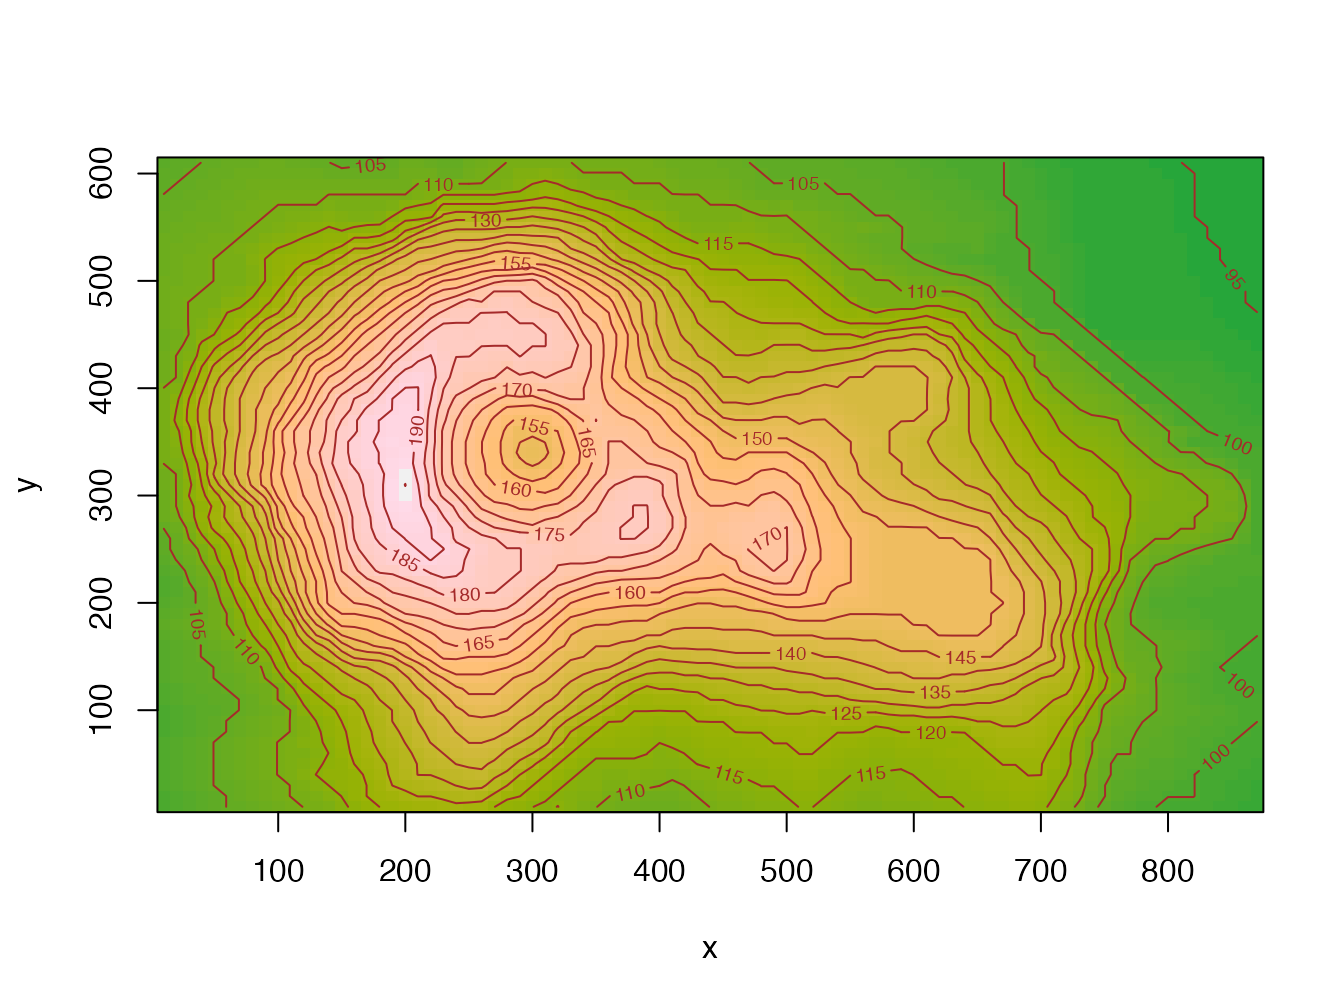
\includegraphics[width=0.8\linewidth]{WwR_files/figure-latex/volcano-1} 

}

\caption{Maunga Whau volcano contours, code provided as an example of the \texttt{image()} function help.}\label{fig:volcano}
\end{figure}

\normalsize

It is composed of a set of colored rectangles: it is indeed a vector image.

If necessary, images can be produced in BMP (bitmap, without compression), JPEG (compressed with loss of quality), PNG (compressed without loss of quality, with possible transparency) or Tiff (compressed or not) formats.

\subsection{Functions}\label{functions}

ggplots can be saved to a file by the \texttt{ggsave()} function.
The extension of the file name sets its format.
See the help of the function for more details.

Other graphics require another method.
The \texttt{postscript()} function produces an EPS file.
The R code must call the function to create the file, produce the figure, and then close the file, for example:

\scriptsize

\begin{Shaded}
\begin{Highlighting}[]
\CommentTok{\# Open the file}
\FunctionTok{postscript}\NormalTok{(}\StringTok{"Fig1.eps"}\NormalTok{, }\AttributeTok{width =} \DecValTok{6}\NormalTok{, }\AttributeTok{height =} \DecValTok{4}\NormalTok{, }\AttributeTok{horizontal =} \ConstantTok{FALSE}\NormalTok{)}
\CommentTok{\# Create the figure}
\FunctionTok{plot}\NormalTok{(cars)}
\CommentTok{\# Close the file}
\FunctionTok{dev.off}\NormalTok{()}
\end{Highlighting}
\end{Shaded}

\begin{verbatim}
## pdf 
##   2
\end{verbatim}

\normalsize

The width and height (in inches) of a vector file are not important, but their ratio fixes the aspect of the figure.
The size of the texts is fixed: increasing the size of the figure means decreasing the relative size of the texts: proceed by successive attempts, making sure that the legends remain readable at the final size of the figure.

The \texttt{horizontal} argument sets the orientation of the figure in a rather unpredictable way: proceed by trials.

The functions \texttt{eps()}, \texttt{pdf()}, \texttt{bmp()}, \texttt{jpeg()}, \texttt{png()} and \texttt{tiff()} work the same way.
Refer to the function help for the choice of options (resolution, compression level, etc.).
The \texttt{emf()} function is provided by the \textbf{devEMF} package.

Fonts are not included in EPS or PDF files.
If necessary, the \texttt{embedFonts()} function can be used to remedy this, provided that GhostScript is installed.

\subsection{ragg package}\label{ragg-package}

The \textbf{ragg}\footnote{\url{https://ragg.r-lib.org/}} package improves the quality of PNG, JPEG and TIFF files.
The optimized functions are \texttt{agg\_png()}, \texttt{agg\_jpeg()} and \texttt{agg\_tiff()}.
Their usage is the same as that of the \textbf{grDevices} functions.

Markdown R documents produce PNG images for their HTML version.
\textbf{ragg} improves their quality: the package must be installed and \texttt{dev\ =\ "ragg\_png"} must be added to the \textbf{knitr} options.
For this document, the options declared in \texttt{index.Rmd} are the following:

\scriptsize

\begin{Shaded}
\begin{Highlighting}[]
\CommentTok{\# knitr options}
\NormalTok{knitr}\SpecialCharTok{::}\NormalTok{opts\_chunk}\SpecialCharTok{$}\FunctionTok{set}\NormalTok{(}
  \AttributeTok{cache =}   \ConstantTok{FALSE}\NormalTok{,    }\CommentTok{\# Cache chunk results}
  \AttributeTok{include =} \ConstantTok{TRUE}\NormalTok{,     }\CommentTok{\# Show/Hide chunks}
  \AttributeTok{echo =}    \ConstantTok{TRUE}\NormalTok{,     }\CommentTok{\# Show/Hide code}
  \AttributeTok{warning =} \ConstantTok{FALSE}\NormalTok{,    }\CommentTok{\# Show/Hide warnings}
  \AttributeTok{message =} \ConstantTok{FALSE}\NormalTok{,    }\CommentTok{\# Show/Hide messages}
  \CommentTok{\# Figure alignment and size}
  \AttributeTok{fig.align =} \StringTok{\textquotesingle{}center\textquotesingle{}}\NormalTok{, }\AttributeTok{out.width =} \StringTok{\textquotesingle{}80\%\textquotesingle{}}\NormalTok{, }\AttributeTok{fig.asp =}\NormalTok{ .}\DecValTok{75}\NormalTok{,}
  \CommentTok{\# Graphic devices (ragg\_png is better than standard png)}
  \AttributeTok{dev =} \FunctionTok{c}\NormalTok{(}\StringTok{"ragg\_png"}\NormalTok{, }\StringTok{"pdf"}\NormalTok{),}
  \CommentTok{\# Code chunk format}
  \AttributeTok{tidy =} \ConstantTok{FALSE}\NormalTok{, }\AttributeTok{tidy.opts =} \FunctionTok{list}\NormalTok{(}\AttributeTok{blank =} \ConstantTok{FALSE}\NormalTok{, }\AttributeTok{width.cutoff =} \DecValTok{60}\NormalTok{),}
  \AttributeTok{size =} \StringTok{"scriptsize"}\NormalTok{, }\AttributeTok{knitr.graphics.auto\_pdf =} \ConstantTok{TRUE}
\NormalTok{  )}
\FunctionTok{options}\NormalTok{(}\AttributeTok{width =} \DecValTok{60}\NormalTok{)}
\end{Highlighting}
\end{Shaded}

\normalsize

Finally, \textbf{ragg} can be used as the default graphics renderer in RStudio starting with version 1.4 (Menu \enquote{Tools \textgreater{} Global Options \textgreater{} General \textgreater{} Graphics \textgreater{} Backend}).

\section{Workflow}\label{sec:targetsmd}

A workflow (see section \ref{sec:targets}) can be embedded in an R Markdown document starting with version 0.5 of the \textbf{targets} package.

\scriptsize

\begin{Shaded}
\begin{Highlighting}[]
\FunctionTok{library}\NormalTok{(}\StringTok{"targets"}\NormalTok{)}
\end{Highlighting}
\end{Shaded}

\normalsize

\subsection{Declaration of the workflow}\label{declaration-of-the-workflow}

The workflow is managed by code snippets of type \texttt{targets}.
Their minimal header is \texttt{\{targets\}} instead of \texttt{\{r\}}, and they must be named.
These code snippets are used to create the \texttt{\_targets.R} file when they are run in non-interactive mode, namely while the document is being knitted.
If they are run in interactive mode, for example in R Studio, their code is executed.
The \texttt{tar\_interactive\ =\ FALSE} option in their header allows them to be tested without knitting the whole document.

Any old workflow must be removed before writing the new one:

\scriptsize

\begin{Shaded}
\begin{Highlighting}[]
\FunctionTok{tar\_unscript}\NormalTok{()}
\end{Highlighting}
\end{Shaded}

\normalsize

The first code chunk, with the \texttt{tar\_globals=TRUE} option, writes the global options for the workflow
To create the workflow shown in section \ref{sec:targets}, the code is simply:

\begin{verbatim}
```{targets targets_global, tar_globals=TRUE}
# Packages
tar_option_set(packages = c("spatstat", "dbmss"))
```
\end{verbatim}

The functions used by the targets are declared in this type of code snippet: they are added to a file in the \texttt{\_targets\_r} working folder (different from the \texttt{\_targets} folder which contains the target calculation files).

\subsection{Declaration of targets}\label{declaration-of-targets}

The targets themselves are declared in code snippets whose name is that of the destination variable.

\begin{verbatim}
```{targets X, tar_simple=TRUE}
runifpoint(n_points)
```
\end{verbatim}

Each target requires a piece of code built in this way.
The value of the target is the last value returned, just like a function that would not use \texttt{return()}.

During knitting, this simplified code (\texttt{tar\_simple=TRUE}) is automatically transformed into a target code:

\scriptsize

\begin{Shaded}
\begin{Highlighting}[]
\FunctionTok{tar\_target}\NormalTok{(X, \{}
  \FunctionTok{runifpoint}\NormalTok{(n\_points)}
\NormalTok{\})}
\end{Highlighting}
\end{Shaded}

\normalsize

The document readability is impaired by this particular syntax: \textbf{targets} is not useful for documents whose code, quick to execute, must be displayed in the text.
On the other hand, if the code is long to execute and is not displayed, it is of considerable interest to limit the computation time.

The other bits of code needed to complete the flow are the following:

\begin{itemize}
\tightlist
\item
  \texttt{n\_points}:
\end{itemize}

\scriptsize

\begin{Shaded}
\begin{Highlighting}[]
\FunctionTok{tar\_target}\NormalTok{(n\_points, \{}
    \DecValTok{1000}
\NormalTok{\})}
\end{Highlighting}
\end{Shaded}

\normalsize

\begin{itemize}
\tightlist
\item
  \texttt{d}:
\end{itemize}

\scriptsize

\begin{Shaded}
\begin{Highlighting}[]
\FunctionTok{tar\_target}\NormalTok{(d, \{}
    \FunctionTok{sum}\NormalTok{(}\FunctionTok{pairdist}\NormalTok{(X)) }\SpecialCharTok{/}\NormalTok{ n\_points }\SpecialCharTok{/}\NormalTok{ (n\_points }\SpecialCharTok{{-}} \DecValTok{1}\NormalTok{)}
\NormalTok{\})}
\end{Highlighting}
\end{Shaded}

\normalsize

\begin{itemize}
\tightlist
\item
  \texttt{map}:
\end{itemize}

\scriptsize

\begin{Shaded}
\begin{Highlighting}[]
\FunctionTok{tar\_target}\NormalTok{(map, \{}
    \FunctionTok{autoplot}\NormalTok{(}\FunctionTok{as.wmppp}\NormalTok{(X))}
\NormalTok{\})}
\end{Highlighting}
\end{Shaded}

\normalsize

\subsection{Running the workflow}\label{running-the-workflow}

To start the target calculation, a standard piece of code (\texttt{\{r\}}) must call \texttt{tar\_make()}:

\scriptsize

\begin{Shaded}
\begin{Highlighting}[]
\FunctionTok{tar\_visnetwork}\NormalTok{()}
\end{Highlighting}
\end{Shaded}

\begin{Shaded}
\begin{Highlighting}[]
\FunctionTok{tar\_make}\NormalTok{()}
\end{Highlighting}
\end{Shaded}

\begin{verbatim}
## ▶ dispatched target n_points
## ● completed target n_points [0.766 seconds, 53 bytes]
## ▶ dispatched target X
## ● completed target X [0.002 seconds, 11.059 kilobytes]
## ▶ dispatched target d
## ● completed target d [0.006 seconds, 55 bytes]
## ▶ dispatched target map
## ● completed target map [0.012 seconds, 187.39 kilobytes]
## ▶ ended pipeline [0.89 seconds]
\end{verbatim}

\normalsize

\texttt{tar\_visnetwork()} is used to check that the workflow is correct before running it.
When the document is finally produced, the \texttt{include=FALSE} option can be added to the header of this piece of code so that it does not produce any output.

\subsection{Using the results}\label{using-the-results}

Code snippets that use target values must read them with \texttt{tar\_read()}:

\scriptsize

\begin{Shaded}
\begin{Highlighting}[]
\FunctionTok{tar\_read}\NormalTok{(map)}
\end{Highlighting}
\end{Shaded}

\begin{center}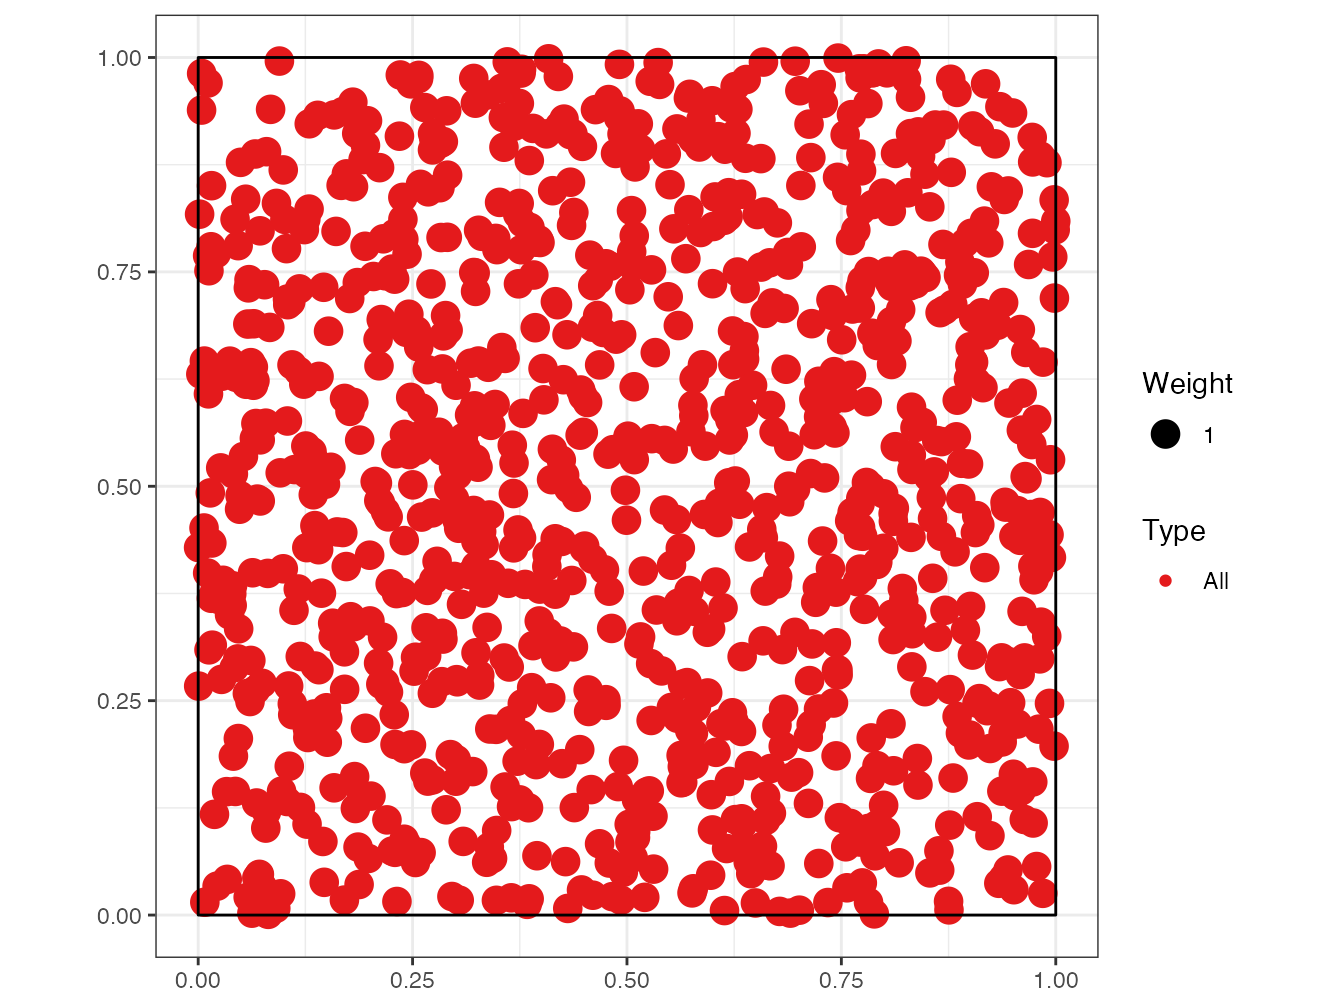
\includegraphics[width=0.8\linewidth]{WwR_files/figure-latex/tar_read_4-1} \end{center}

\normalsize

\subsection{Source control}\label{source-control-1}

The \textbf{targets} files must be included in the source control.
This way, calculations done locally will not be repeated by GitHub Actions (chapter \ref{chap-ci}) and building the document will be fast.

\chapter{Package}\label{chap-package}

\toc{1}

R packages extend its functionality with code provided by the developer community.
They are the key to the success of R because they allow to quickly spread new methods resulting from research or to add new tools that can become standards, such as the \textbf{tidyverse}.

It is useful to produce a package when you have written new functions that form a coherent whole.
A package for personal use or limited to a work team is simple to set up and the time saved by easily using the updated version of each function very quickly amortizes the time spent on making the package.
This type of package is intended to be hosted on GitHub.

Packages with a wider use, which provide for example the code corresponding to a published method, are placed in the CRAN repository, from where they can be installed by the standard command \texttt{install.packages()}.
CRAN performs extensive code checks and only accepts packages that pass its test suite without any warning.
They must respect the policies\footnote{\url{https://cran.r-project.org/web/packages/policies.html}} of the repository.

The documentation for package creation is abundant.
The reference book is \textcite{Wickham2015}, which should be consulted as a reference.

The approach used here is to create a first package very quickly to understand that the process is quite simple.
It will then be enriched with the elements necessary for a package distributed to other users than its designer: a complete documentation and tests of correct operation in particular.

\section{First package}\label{first-package}

This introduction follows the recommendations of the blog \emph{Creating a package in minutes}\footnote{\url{https://thinkr.fr/creer-package-r-quelques-minutes/}} from ThinkR.

\subsection{Creation}\label{creation}

Packages have a strict organization in a fixed file and directory structure.
It is possible to create this structure manually but specialized packages can do it:

\begin{itemize}
\tightlist
\item
  \textbf{usethis} automates the creation of folders.
\item
  \textbf{roxygen2} automates the mandatory documentation of packages.
\item
  \textbf{devtools} is the developer's toolbox, allowing to build and test packages.
\end{itemize}

All three are to be installed first:

\scriptsize

\begin{Shaded}
\begin{Highlighting}[]
\FunctionTok{install.packages}\NormalTok{(}\FunctionTok{c}\NormalTok{(}\StringTok{"usethis"}\NormalTok{, }\StringTok{"roxygen2"}\NormalTok{, }\StringTok{"devtools"}\NormalTok{))}
\end{Highlighting}
\end{Shaded}

\normalsize

The package to create will be an RStudio project.
In the project menu, select \enquote{New Project \textgreater{} New Directory \textgreater{} R package using devtools\ldots{}}, choose the name of the project and its parent folder.
The package will be called \textbf{multiple}, in the \texttt{\%LOCALAPPDATA\%\textbackslash{}ProjectsR} folder, following the recommendations in the section \ref{sec:solution-dossiers}.

The name of the package must respect the constraints of project names: no special characters, no spaces\ldots{}
It must also be evocative of the purpose of the package.
If the package is to be distributed, all its documentation will be written in English, including its name.

The minimal structure is created:

\begin{itemize}
\tightlist
\item
  A \texttt{DESCRIPTION} file which indicates that the folder contains a package and specifies at least its name.
\item
  A \texttt{NAMESPACE} file which declares how the package intervenes in the management of the names of R objects (its content will be updated by \textbf{roxygen2}).
\item
  An \texttt{R} file which contains the code of the functions offered by the package (empty at this stage).
\end{itemize}

The package can be tested right away: in the RStudio \emph{Build} window, clicking on \enquote{Install and Restart} builds the package and loads it into R, after restarting the program to avoid any conflicts.

In the \emph{Packages} window, \textbf{multiple} is now visible.
It is loaded, but contains nothing.

\subsection{First function}\label{first-function}

\subsubsection{Files}\label{files}

Functions are placed in one or more \texttt{.R} files in the \texttt{R} folder.
The organization of these files is free.
For this example, a file with the name of each function will be created.
Files grouping similar functions or a single file containing all the code are possible choices.

The choice made here is the following:

\begin{itemize}
\tightlist
\item
  A file that will contain the code common to the whole package: \texttt{package.R}.
\item
  One file common to all functions: \texttt{functions.R}.
\end{itemize}

\subsubsection{Creation}\label{creation-1}

The first function, \texttt{double()}, is created and stored in the \texttt{functions.R} file:

\scriptsize

\begin{Shaded}
\begin{Highlighting}[]
\NormalTok{double }\OtherTok{\textless{}{-}} \ControlFlowTok{function}\NormalTok{(number) \{}
  \FunctionTok{return}\NormalTok{(}\DecValTok{2} \SpecialCharTok{*}\NormalTok{ number)}
\NormalTok{\}}
\end{Highlighting}
\end{Shaded}

\normalsize

At this point, the function is internal to the package and is not accessible from the working environment.
To be sure, build the package (\emph{Install and Restart}) and check that the function works:

\scriptsize

\begin{Shaded}
\begin{Highlighting}[]
\FunctionTok{double}\NormalTok{(}\DecValTok{2}\NormalTok{)}
\end{Highlighting}
\end{Shaded}

\begin{verbatim}
## [1] 4
\end{verbatim}

\normalsize

The result is a vector composed of two 0's because the called function is a homonym of the \textbf{base} package (see its documentation by typing \texttt{?double}):

\scriptsize

\begin{Shaded}
\begin{Highlighting}[]
\NormalTok{base}\SpecialCharTok{::}\FunctionTok{double}\NormalTok{(}\DecValTok{2}\NormalTok{)}
\end{Highlighting}
\end{Shaded}

\begin{verbatim}
## [1] 0 0
\end{verbatim}

\normalsize

In order for the function in our package to be visible, it must be \emph{exported} by declaring it in the \texttt{NAMESPACE} file.
This is the job of \textbf{roxygen2} which manages the documentation of each function at the same time.
To activate it, place the cursor in the function and call the menu \enquote{Code \textgreater{} Insert Roxygen Skeleton}.
Comments are added before the function:

\scriptsize

\begin{Shaded}
\begin{Highlighting}[]
\CommentTok{\#\textquotesingle{} Title}
\CommentTok{\#\textquotesingle{}}
\CommentTok{\#\textquotesingle{} @param number }
\CommentTok{\#\textquotesingle{}}
\CommentTok{\#\textquotesingle{} @return}
\CommentTok{\#\textquotesingle{} @export}
\CommentTok{\#\textquotesingle{}}
\CommentTok{\#\textquotesingle{} @examples}
\NormalTok{double }\OtherTok{\textless{}{-}} \ControlFlowTok{function}\NormalTok{(number) \{}
  \FunctionTok{return}\NormalTok{(}\DecValTok{2} \SpecialCharTok{*}\NormalTok{ number)}
\NormalTok{\}}
\end{Highlighting}
\end{Shaded}

\normalsize

Comments to \textbf{roxygen2} begin with \texttt{\#\textquotesingle{}}:

\begin{itemize}
\tightlist
\item
  The first line contains the title of the function, i.e.~a very short description: its name in general.
\item
  The next line (separated by a line break) may contain its description (see \emph{Description} in the help).
\item
  The next line (after another line break) might contain more information (\emph{Details} in the help).
\item
  The arguments of the function are described by the \texttt{@param} lines.
\item
  \texttt{@return} describes the result of the function.
\item
  \texttt{@export} declares that the function is exported: it will be usable in the working environment.
\item
  Examples can be added.
\end{itemize}

The documentation must be completed:

\scriptsize

\begin{Shaded}
\begin{Highlighting}[]
\CommentTok{\#\textquotesingle{} double}
\CommentTok{\#\textquotesingle{} }
\CommentTok{\#\textquotesingle{} Double value of numbers.}
\CommentTok{\#\textquotesingle{}}
\CommentTok{\#\textquotesingle{} Calculate the double values of numbers.}
\CommentTok{\#\textquotesingle{} }
\CommentTok{\#\textquotesingle{} @param number a numeric vector.}
\CommentTok{\#\textquotesingle{}}
\CommentTok{\#\textquotesingle{} @return A vector of the same length as \textasciigrave{}number\textasciigrave{} containing the }
\CommentTok{\#\textquotesingle{}   transformed values.}
\CommentTok{\#\textquotesingle{} @export}
\CommentTok{\#\textquotesingle{}}
\CommentTok{\#\textquotesingle{} @examples}
\CommentTok{\#\textquotesingle{} double(2)}
\CommentTok{\#\textquotesingle{} double(1:4)}
\NormalTok{double }\OtherTok{\textless{}{-}} \ControlFlowTok{function}\NormalTok{(number) \{}
  \FunctionTok{return}\NormalTok{(}\DecValTok{2} \SpecialCharTok{*}\NormalTok{ number)}
\NormalTok{\}}
\end{Highlighting}
\end{Shaded}

\normalsize

Don't hesitate to use the help of existing functions to respect R standards (here: \texttt{?log}):

\begin{itemize}
\tightlist
\item
  Keep in mind that functions are normally vector: \texttt{number} is by default a vector, not a scalar.
\item
  Some elements start with a capital letter and end with a dot because they are paragraphs in the help file.
\item
  The title does not have a period.
\item
  The description of the parameters does not start with a capital letter.
\end{itemize}

Taking into account the changes in the documentation requires calling the \texttt{roxygenize()} function.
In the \emph{Build} window, the \enquote{More \textgreater{} Document} menu allows you to do this.
Then build the package (\emph{Install and Restart}) and check the result by running the function and displaying its help:

\scriptsize

\begin{Shaded}
\begin{Highlighting}[]
\FunctionTok{double}\NormalTok{(}\DecValTok{2}\NormalTok{)}
\NormalTok{?double}
\end{Highlighting}
\end{Shaded}

\normalsize

It is possible to automate the update of the documentation at each build of the package by the menu \enquote{Build \textgreater{} Configure Build Tools\ldots{}}: click on \enquote{Configure} and check the box \enquote{Automatically reoxygenize when running Install and Restart}.
This is an efficient choice for a small package but penalizing when the time to update the documentation increases with the complexity of the package. The package rebuild is most often used to test code changes: its speed is essential.

The documentation for \textbf{roxygen2} supports the Markdown\footnote{\url{https://roxygen2.r-lib.org/articles/markdown.html}} format.

At this stage, the package is functional: it contains a function and a beginning of documentation.
It is time to run a check of its code: in the \emph{Build} window, click on \enquote{Check} or use the \texttt{devtools::check()} command.
The operation \emph{reoxygenates} the package (updates its documentation), performs a large number of tests and returns a list of errors, warnings and notes detected.
The goal is always to have no warnings: they must be handled immediately.
For example, the following return is a warning about the non-conformity of the declared license:

\begin{verbatim}
> checking DESCRIPTION meta-information ... WARNING
  Non-standard license specification:
    `use_gpl3_license()`
  Standardizable: FALSE

0 errors v | 1 warning x | 0 notes v
Erreur : R CMD check found WARNINGs
\end{verbatim}

To correct it, update, run the update license command, starting with your name:

\scriptsize

\begin{Shaded}
\begin{Highlighting}[]
\FunctionTok{options}\NormalTok{(}\AttributeTok{usethis.full\_name =} \StringTok{"Eric Marcon"}\NormalTok{)}
\NormalTok{usethis}\SpecialCharTok{::}\FunctionTok{use\_gpl3\_license}\NormalTok{()}
\end{Highlighting}
\end{Shaded}

\normalsize

The list of valid licenses is provided by R\footnote{\url{https://svn.r-project.org/R/trunk/share/licenses/license.db}}.

After correction, run the tests again until the alerts disappear.

\subsection{Source control}\label{sec:package-cds}

It is time to put the code under source control.

Enable source control in the project options (figure \ref{fig:git-Project}).
Restart RStudio on demand.

Create a repository on GitHub and push the local repository to it, as explained in the chapter \ref{chap-git}.

Create the file \texttt{README.md}:

\begin{verbatim}
# multiple

An R package to compute mutiple of numbers.
\end{verbatim}

The development of the package is punctuated by many commits at each modification and a push at each step, validated by a version number increment.

\subsection{package.R}\label{package.r}

The \texttt{package.R} file is intended to receive the R code and especially the comments for \textbf{roxygen2} which concern the whole package.
This file can also be named \texttt{multiple-package.R}, prefixed with the package name, for compatibility with \textbf{usethis}.
It can be created under this name with the command:

\scriptsize

\begin{Shaded}
\begin{Highlighting}[]
\NormalTok{usethis}\SpecialCharTok{::}\FunctionTok{use\_package\_doc}\NormalTok{()}
\end{Highlighting}
\end{Shaded}

\normalsize

The first comment block will generate the package help (\texttt{?multiple}).

\begin{verbatim}
#' @keywords internal 
"_PACKAGE"
\end{verbatim}

The ``\_PACKAGE'' keyword indicates that package documentation must be produced.
It could be written in the block, with a syntax identical to that of functions, but its default content is that of the \texttt{Description} field in the \texttt{DESCRIPTION} file.
The \texttt{internal} keyword hides the package documentation in the help summary.

The documentation is updated by the \texttt{roxygen2::roxygenise()} command.
After rebuilding the package, check that the help has appeared: \texttt{?multiple}.

\section{Package organization}\label{package-organization}

\subsection{DESCRIPTION file}\label{sec:package-description}

The file must be completed:

\begin{verbatim}
Package: multiple
Title: Calculate multiples of numbers
Version: 0.0.0.9000
Authors@R: 
  person(given = "Eric",
           family = "Marcon",
           role = c("aut", "cre"),
           email = "e.marcon@free.fr",
           comment = c(ORCID = "0000-0002-5249-321X"))
Description: Simple computation of multiples of numbers, 
  including fast algorithms for integers.
License: GPL-3
Encoding: UTF-8
LazyData: true
Roxygen: list(markdown = TRUE)
RoxygenNote: 7.1.1
\end{verbatim}

The package name is fixed and must not be changed.

Its title must describe in one line what it is used for.
The title is displayed in the \emph{Packages} window next to the package names.

The version must respect the conventions:

\begin{itemize}
\tightlist
\item
  The first number is the major version, 0 as long as the package is not stable, then 1.
  The major version only changes if the package is no longer compatible with its previous versions, which forces users to modify their code.
\item
  The second is the minor version, incremented when new features are added.
\item
  The third is the correction version: 0 at the origin, incremented at each code correction without new functionality.
\item
  The fourth is reserved for development, and starts at 9000.
  It is incremented with each unstable version and disappears when a new stable version (\emph{release}) is produced.
\end{itemize}

Example: a bug fix on version 1.3.0 produces version 1.3.1.
The following development versions (unstable, not intended for production use) are 1.3.1.9000 then 1.3.1.9001, etc.
The version number must be updated each time the package is pushed on GitHub.
When the development is stabilized, the new version, intended to be used in production, is 1.3.2 if it does not bring any new functionality or 1.4.0 in the opposite case.

The description of the authors is rather heavy but simple to understand.
The Orcid identifiers of academic authors can be used.
If the package has several authors, they are placed in a \texttt{c()} function: \texttt{c(person(...),\ person(...))} for two authors.
In this case, the role of each must be specified:

\begin{itemize}
\tightlist
\item
  \enquote{cre} for the creator of the package.
\item
  \enquote{aut} for one of the other authors.
\item
  \enquote{ctb} for a contributor, who may have reported a bug or provided some code.
\end{itemize}

The description of the package in one paragraph allows to give more information.

The license specifies how the package can be used and modified.
GPL-3 is a good default, but other choices are possible\footnote{\url{https://r-pkgs.org/description.html\#description-license}}.

The \texttt{LazyData} option means that the example data provided with the package can be used without calling it first by the \texttt{data()} function: this is the current standard.

Finally, the last two lines are handled by \textbf{roxygen2}.

\subsection{NEWS.md file}\label{news.md-file}

The \texttt{NEWS.md} file contains the history of the package.
New versions are added to the top of the file.

Create a first version of the file:

\begin{verbatim}
# multiple 0.0.0.9000

## New features

* Initial version of the package
\end{verbatim}

The first level titles must contain the package name and version.
Level 2 titles are free, but usually contain headings like \enquote{New features} and \enquote{Bug Fixes}.

To avoid multiplying the versions described, it is advisable to change the current version and complete the documentation until the correction version changes (third number).
Then, the entry corresponding to this version remains frozen and a new entry is added.

\section{Vignette}\label{vignette}

A vignette is essential to document the package correctly:

\scriptsize

\begin{Shaded}
\begin{Highlighting}[]
\NormalTok{usethis}\SpecialCharTok{::}\FunctionTok{use\_vignette}\NormalTok{(}\StringTok{"multiple"}\NormalTok{)}
\end{Highlighting}
\end{Shaded}

\normalsize

The file \texttt{multiple.Rmd} is created in the \texttt{vignette} folder.
Add a subtitle in its header: the short description of the package:

\begin{verbatim}
title: "multiple"
subtitle: "Multiples of numbers"
\end{verbatim}

The rest of the header allows R to build the vignette from R Markdown code.

The body of the vignette contains by default R code to declare the options for presenting the code snippets and loading the package.
An introduction to the use of the package should be written in this document, in R Markdown.

During the development of the package, the vignette can be built manually by running:

\scriptsize

\begin{Shaded}
\begin{Highlighting}[]
\NormalTok{devtools}\SpecialCharTok{::}\FunctionTok{build\_vignettes}\NormalTok{(}\StringTok{"multiple"}\NormalTok{) }
\end{Highlighting}
\end{Shaded}

\normalsize

The resulting files are placed in \texttt{doc/}: open the \texttt{.html} file to check the result.

RStudio does not create the package vignette when the \enquote{Install and Restart} command in the Build window is called.
For a complete installation, two solutions are possible:

\begin{itemize}
\tightlist
\item
  Build the package source file (\enquote{Build \textgreater{} More \textgreater{} Build Source Package}) and then install it (\enquote{Packages \textgreater{} Install \textgreater{} Install from \textgreater{} Package Archive file}).
  The source file is next to the project file.
\item
  Push the package code on GitHub and then run:
\end{itemize}

\scriptsize

\begin{Shaded}
\begin{Highlighting}[]
\NormalTok{remotes}\SpecialCharTok{::}\FunctionTok{install\_github}\NormalTok{(}\StringTok{"multiple"}\NormalTok{, }\AttributeTok{build\_vignettes =} \ConstantTok{TRUE}\NormalTok{)}
\end{Highlighting}
\end{Shaded}

\normalsize

The vignette can then be displayed by the command:

\scriptsize

\begin{Shaded}
\begin{Highlighting}[]
\FunctionTok{vignette}\NormalTok{(}\StringTok{"multiple"}\NormalTok{)}
\end{Highlighting}
\end{Shaded}

\normalsize

\section{pkgdown}\label{pkgdown}

The \textbf{pkgdown} package creates a companion site to the package\footnote{Example: \url{https://EricMarcon.github.io/entropart/}}, which includes the \texttt{README.md} file as the home page, the vignette in a \enquote{Get Started} section, all of the help files with their executed examples (the \enquote{Reference} section), the \texttt{NEWS.md} file for a history of the package (the \enquote{Changelog} section), and information from the \texttt{DESCRIPTION} file.

Create the site with \textbf{usethis}:

\scriptsize

\begin{Shaded}
\begin{Highlighting}[]
\NormalTok{usethis}\SpecialCharTok{::}\FunctionTok{use\_pkgdown}\NormalTok{()}
\end{Highlighting}
\end{Shaded}

\normalsize

Then build the site.
This command will be executed again at each version change of the package:

\scriptsize

\begin{Shaded}
\begin{Highlighting}[]
\NormalTok{pkgdown}\SpecialCharTok{::}\FunctionTok{build\_site}\NormalTok{()}
\end{Highlighting}
\end{Shaded}

\normalsize

The site is placed in the \texttt{docs} folder.
Open the file \texttt{index.htm} with a web browser to view it.
As soon as the project is pushed to GitHub, activate the repository pages so that the site is visible online (see section \ref{sec:github-pages}).

\textbf{pkgdown} places the site in the \texttt{docs} folder.

Add the address of the GitHub pages to a new line in the \texttt{DESCRIPTION} file:

\begin{verbatim}
URL: https://GitHubID.github.io/multiple
\end{verbatim}

Also add it to the \texttt{\_pkgdown.yml} file that was created empty, along with the following option:

\begin{verbatim}
url: https://GitHubID.github.io/multiple

development:
  mode: auto
\end{verbatim}

\textbf{pkgdown} places the site in the \texttt{docs/dev} folder if the site for a stable (three-numbered) version of the package exists in \texttt{docs} and the current version is a development version (four-numbered).
This way, users of a production version of the package have access to the site without it being disturbed by the development versions.

The site can be enriched in several ways:

\begin{itemize}
\tightlist
\item
  By adding articles in R Markdown format to the \texttt{vignettes/articles} folder.
  The vignette should not require significant computational resources to present examples because it is built at the same time as the package.
  The articles are generated by \textbf{pkgdown}, independently, and can therefore be more ambitious;
\item
  By improving its presentation (grouping functions by themes, adding badges, a sticker\footnote{The Shiny application \textbf{hexmake} allows easy creation of a sticker: \url{https://connect.thinkr.fr/hexmake/}}\ldots): refer to the help of \textbf{pkgdown}.
\end{itemize}

To enrich the documentation of the package, it is possible to use a \texttt{README.Rmd} file in R Markdown format, to be knitted to create the standard \texttt{README.md} of GitHub, used as the home page of the \textbf{pkgdown} site, which can in this way present examples of use of the code.
The approach is detailed in \emph{R Packages}\footnote{\url{https://r-pkgs.org/release.html?q=readme\#readme-rmd}}.
The added complexity is to be compared to the gain: a simple homepage (without code) with links to the vignette and articles is easier to implement.

\section{Package specific code}\label{package-specific-code}

\subsection{Importing functions}\label{importing-functions}

Let's create a new function in \texttt{functions.R} that adds random noise to the double value:

\scriptsize

\begin{Shaded}
\begin{Highlighting}[]
\NormalTok{fuzzydouble }\OtherTok{\textless{}{-}} \ControlFlowTok{function}\NormalTok{(number, }\AttributeTok{sd =} \DecValTok{1}\NormalTok{) \{}
  \FunctionTok{return}\NormalTok{(}\DecValTok{2} \SpecialCharTok{*}\NormalTok{ number }\SpecialCharTok{+} \FunctionTok{rnorm}\NormalTok{(}\FunctionTok{length}\NormalTok{(number), }\DecValTok{0}\NormalTok{, sd))}
\NormalTok{\}}
\end{Highlighting}
\end{Shaded}

\normalsize
The noise is drawn in a centered normal distribution of standard deviation \texttt{sd} and added to the calculated value.

\texttt{rnorm()} is a function of the \textbf{stats} package.
Even though the package is systematically loaded by R, the package to which the function belongs must be declared: the only exceptions are functions from the \textbf{base} package.

The \textbf{stats} package must first be declared in \texttt{DESCRIPTION} which contains an \texttt{Imports:} statement.
All packages used by the \textbf{multiple} code will be listed, separated by commas.

\begin{verbatim}
Imports: stats
\end{verbatim}

This \enquote{import} simply means that the \textbf{stats} package must be loaded, but not necessarily attached (see section \ref{sec:environnements}), for \textbf{multiple} to work.

Then, the \texttt{rnorm()} function must be found in the \textbf{multiple} package environment.
There are several ways to fulfill this requirement.
First, the following comment could be provided for \textbf{roxygen2}:

\scriptsize

\begin{Shaded}
\begin{Highlighting}[]
\CommentTok{\#\textquotesingle{} @import stats}
\end{Highlighting}
\end{Shaded}

\normalsize

The entire namespace of the \textbf{stats} package would be attached to and accessible by the \textbf{multiple} package.
This is not a good practice because it inreases the risk of name conflicts (see section \ref{sec:environnements}).
Note that the notion of import used here is different from that of \texttt{DESCRIPTION}, although they have the same name.

It is best to import only the \texttt{rnorm()} function by declaring it in the function documentation:

\scriptsize

\begin{Shaded}
\begin{Highlighting}[]
\CommentTok{\#\textquotesingle{} @importFrom stats rnorm}
\end{Highlighting}
\end{Shaded}

\normalsize

This is not an ideal practice either because the origin of the function would not be clear in the package code.

The best practice is to import nothing (in the sense of \textbf{roxygen2}) and to systematically qualify functions from other packages with the syntax \texttt{package::function()}.
This is the solution chosen here because the \texttt{@importFrom} directive would import the function in the whole \textbf{multiple} package, not only in the \texttt{fuzzydouble()} function, at the risk of creating side effects (modifying the behavior of another function of the package which would not assume the import of \texttt{rnorm()}).
Finally, the code of the function is as follows:

\scriptsize

\begin{Shaded}
\begin{Highlighting}[]
\CommentTok{\#\textquotesingle{} fuzzydouble}
\CommentTok{\#\textquotesingle{} }
\CommentTok{\#\textquotesingle{} Double value of numbers with an error}
\CommentTok{\#\textquotesingle{} }
\CommentTok{\#\textquotesingle{} Calculate the double values of numbers }
\CommentTok{\#\textquotesingle{} and add a random error to the result.}
\CommentTok{\#\textquotesingle{}}
\CommentTok{\#\textquotesingle{} @param number a numeric vector.}
\CommentTok{\#\textquotesingle{} @param sd the standard deviation of the Gaussian error added.}
\CommentTok{\#\textquotesingle{}}
\CommentTok{\#\textquotesingle{} @return A vector of the same length as \textasciigrave{}number\textasciigrave{}}
\CommentTok{\#\textquotesingle{}  containing the transformed values.}
\CommentTok{\#\textquotesingle{} @export}
\CommentTok{\#\textquotesingle{}}
\CommentTok{\#\textquotesingle{} @examples}
\CommentTok{\#\textquotesingle{} fuzzydouble(2)}
\CommentTok{\#\textquotesingle{} fuzzydouble(1:4)}

\NormalTok{fuzzydouble }\OtherTok{\textless{}{-}} \ControlFlowTok{function}\NormalTok{(number, }\AttributeTok{sd =} \DecValTok{1}\NormalTok{) \{}
  \FunctionTok{return}\NormalTok{(}\DecValTok{2} \SpecialCharTok{*}\NormalTok{ number }\SpecialCharTok{+}\NormalTok{ stats}\SpecialCharTok{::}\FunctionTok{rnorm}\NormalTok{(}\FunctionTok{length}\NormalTok{(number), }\DecValTok{0}\NormalTok{, sd))}
\NormalTok{\}}
\end{Highlighting}
\end{Shaded}

\normalsize

\subsection{S3 methods}\label{s3-methods}

S3 methods are presented in section \ref{sec:S3}.

\subsubsection{Classes}\label{classes}

Objects belong to classes:

\scriptsize

\begin{Shaded}
\begin{Highlighting}[]
\CommentTok{\# Class of a number}
\FunctionTok{class}\NormalTok{(}\DecValTok{2}\NormalTok{)}
\end{Highlighting}
\end{Shaded}

\begin{verbatim}
## [1] "numeric"
\end{verbatim}

\begin{Shaded}
\begin{Highlighting}[]
\CommentTok{\# Class of a function}
\FunctionTok{class}\NormalTok{(sum)}
\end{Highlighting}
\end{Shaded}

\begin{verbatim}
## [1] "function"
\end{verbatim}

\normalsize

In addition to the basic classes, developers can create others.

\subsubsection{Methods}\label{methods}

The point of creating new classes is to adapt existing methods to them, the most common case being \texttt{plot()}.
This is a generic method, i.e.~a function template, without code, to be adapted to the class of object to be processed.

\scriptsize

\begin{Shaded}
\begin{Highlighting}[]
\NormalTok{plot}
\end{Highlighting}
\end{Shaded}

\begin{verbatim}
## function (x, y, ...) 
## UseMethod("plot")
## <bytecode: 0x12a9f2550>
## <environment: namespace:base>
\end{verbatim}

\normalsize

There are many variations of \texttt{plot} in R, which are functions with names of the form \texttt{plot.class()}.
\textbf{stats} provides a function \texttt{plot.lm()} to create a figure from a linear model.
Many packages create classes tailored to their objects and provide a \texttt{plot} method for each class.
The functions can be listed:

\scriptsize

\begin{Shaded}
\begin{Highlighting}[]
\CommentTok{\# A few plot() functions}
\FunctionTok{head}\NormalTok{(}\FunctionTok{methods}\NormalTok{(plot))}
\end{Highlighting}
\end{Shaded}

\begin{verbatim}
## [1] "plot,ANY-method"      "plot,color-method"   
## [3] "plot.AccumCurve"      "plot.acf"            
## [5] "plot.ACF"             "plot.adaptivedensity"
\end{verbatim}

\begin{Shaded}
\begin{Highlighting}[]
\CommentTok{\# Total number}
\FunctionTok{length}\NormalTok{(}\FunctionTok{methods}\NormalTok{(plot))}
\end{Highlighting}
\end{Shaded}

\begin{verbatim}
## [1] 156
\end{verbatim}

\normalsize

Conversely, the available methods for a class can be displayed:

\scriptsize

\begin{Shaded}
\begin{Highlighting}[]
\FunctionTok{methods}\NormalTok{(}\AttributeTok{class =} \StringTok{"lm"}\NormalTok{)}
\end{Highlighting}
\end{Shaded}

\begin{verbatim}
##  [1] add1           alias          anova         
##  [4] as_flextable   case.names     coerce        
##  [7] confint        cooks.distance deviance      
## [10] dfbeta         dfbetas        drop1         
## [13] dummy.coef     effects        extractAIC    
## [16] family         formula        fortify       
## [19] hatvalues      influence      initialize    
## [22] kappa          labels         logLik        
## [25] model.frame    model.matrix   nobs          
## [28] plot           predict        print         
## [31] proj           qqnorm         qr            
## [34] residuals      response       rstandard     
## [37] rstudent       show           simulate      
## [40] slotsFromS3    summary        variable.names
## [43] vcov          
## see '?methods' for accessing help and source code
\end{verbatim}

\normalsize

The \texttt{print} method is used to display any object (it is implicit when only the name of an object is entered):

\scriptsize

\begin{Shaded}
\begin{Highlighting}[]
\NormalTok{my\_lm }\OtherTok{\textless{}{-}} \FunctionTok{lm}\NormalTok{(dist }\SpecialCharTok{\textasciitilde{}}\NormalTok{ speed, }\AttributeTok{data =}\NormalTok{ cars)}
\CommentTok{\# Equivalent to "\textgreater{} my\_lm"}
\FunctionTok{print}\NormalTok{(my\_lm)}
\end{Highlighting}
\end{Shaded}

\begin{verbatim}
## 
## Call:
## lm(formula = dist ~ speed, data = cars)
## 
## Coefficients:
## (Intercept)        speed  
##     -17.579        3.932
\end{verbatim}

\normalsize

The \texttt{summary} method displays a readable summary of the object:

\scriptsize

\begin{Shaded}
\begin{Highlighting}[]
\FunctionTok{summary}\NormalTok{(my\_lm)}
\end{Highlighting}
\end{Shaded}

\begin{verbatim}
## 
## Call:
## lm(formula = dist ~ speed, data = cars)
## 
## Residuals:
##     Min      1Q  Median      3Q     Max 
## -29.069  -9.525  -2.272   9.215  43.201 
## 
## Coefficients:
##             Estimate Std. Error t value Pr(>|t|)    
## (Intercept) -17.5791     6.7584  -2.601   0.0123 *  
## speed         3.9324     0.4155   9.464 1.49e-12 ***
## ---
## Signif. codes:  
## 0 '***' 0.001 '**' 0.01 '*' 0.05 '.' 0.1 ' ' 1
## 
## Residual standard error: 15.38 on 48 degrees of freedom
## Multiple R-squared:  0.6511, Adjusted R-squared:  0.6438 
## F-statistic: 89.57 on 1 and 48 DF,  p-value: 1.49e-12
\end{verbatim}

\normalsize

The other methods have been created specifically for the needs of the \textbf{stats} package.

\subsubsection{Assigning an object to a class}\label{assigning-an-object-to-a-class}

In order for an object to belong to a class, it is sufficient to declare it:

\scriptsize

\begin{Shaded}
\begin{Highlighting}[]
\NormalTok{x }\OtherTok{\textless{}{-}} \DecValTok{1}
\FunctionTok{class}\NormalTok{(x) }\OtherTok{\textless{}{-}} \StringTok{"MyClass"}
\FunctionTok{class}\NormalTok{(x)}
\end{Highlighting}
\end{Shaded}

\begin{verbatim}
## [1] "MyClass"
\end{verbatim}

\normalsize

A more elegant way to do this is to add the new class to the set of classes to which the object already belongs:

\scriptsize

\begin{Shaded}
\begin{Highlighting}[]
\NormalTok{y }\OtherTok{\textless{}{-}} \DecValTok{1}
\FunctionTok{class}\NormalTok{(y) }\OtherTok{\textless{}{-}} \FunctionTok{c}\NormalTok{(}\StringTok{"MyClass"}\NormalTok{, }\FunctionTok{class}\NormalTok{(y))}
\FunctionTok{class}\NormalTok{(y)}
\end{Highlighting}
\end{Shaded}

\begin{verbatim}
## [1] "MyClass" "numeric"
\end{verbatim}

\normalsize

There is no consistency check between the real structure of the object and a structure of the class that would be declared elsewhere: the developer must make sure that the methods will find the right data in the objects that declare to belong to it.
If not, errors will occur:

\scriptsize

\begin{Shaded}
\begin{Highlighting}[]
\FunctionTok{class}\NormalTok{(y) }\OtherTok{\textless{}{-}} \StringTok{"lm"}
\FunctionTok{tryCatch}\NormalTok{(}\FunctionTok{print}\NormalTok{(y), }\AttributeTok{error =} \ControlFlowTok{function}\NormalTok{(e) }\FunctionTok{print}\NormalTok{(e))}
\end{Highlighting}
\end{Shaded}

\begin{verbatim}
## <simpleError in x$call: $ operator is invalid for atomic vectors>
\end{verbatim}

\normalsize

\subsection{In practice}\label{in-practice}

\subsubsection{Creating a generic method}\label{creating-a-generic-method}

New generic methods can be created and declined according to the classes.

As an example, let's create a generic method \texttt{triple} which will calculate the triple of numbers in the package \textbf{multiple}, declined in two distinct functions: one for integers and one for reals.
Calculations on integers are faster than those on reals, which justifies (at least in theory) the effort of writing two versions of the code.

\scriptsize

\begin{Shaded}
\begin{Highlighting}[]
\CommentTok{\# Generic Mthod}
\NormalTok{triple }\OtherTok{\textless{}{-}} \ControlFlowTok{function}\NormalTok{(x, ...) \{}
  \FunctionTok{UseMethod}\NormalTok{(}\StringTok{"triple"}\NormalTok{)}
\NormalTok{\}}
\end{Highlighting}
\end{Shaded}

\normalsize

The generic method contains no code beyond its declaration.
Its signature (i.e., the set of arguments) is important because functions derived from this method will necessarily have to have the same arguments in the same order and can only add additional arguments before \texttt{...} (which is mandatory).
As the nature of the first argument will depend on the class of each object, it is usual to call it \texttt{x}.

The method is declined in two functions:

\scriptsize

\begin{Shaded}
\begin{Highlighting}[]
\NormalTok{triple.integer }\OtherTok{\textless{}{-}} \ControlFlowTok{function}\NormalTok{(x, ...)\{}
  \FunctionTok{return}\NormalTok{(x }\SpecialCharTok{*} \DecValTok{3}\DataTypeTok{L}\NormalTok{)}
\NormalTok{\}}
\NormalTok{triple.numeric }\OtherTok{\textless{}{-}} \ControlFlowTok{function}\NormalTok{(x, ...)\{}
  \FunctionTok{return}\NormalTok{(x }\SpecialCharTok{*} \FloatTok{3.0}\NormalTok{)}
\NormalTok{\}}
\end{Highlighting}
\end{Shaded}

\normalsize

In its integer version, \texttt{x} is multiplied by \texttt{3L}, the suffix \texttt{L} meaning that 3 should be understood as an integer.
In its real version, 3 can be written \texttt{3.0} to make it clear that it is a real.
Under R, \texttt{3} without further specification is understood as a real.

The choice of function depends on the class of the object passed as argument.

\scriptsize

\begin{Shaded}
\begin{Highlighting}[]
\CommentTok{\# Integer argument}
\FunctionTok{class}\NormalTok{(}\DecValTok{2}\DataTypeTok{L}\NormalTok{)}
\end{Highlighting}
\end{Shaded}

\begin{verbatim}
## [1] "integer"
\end{verbatim}

\begin{Shaded}
\begin{Highlighting}[]
\CommentTok{\# Integer result by the function triple.integer}
\FunctionTok{class}\NormalTok{(}\FunctionTok{triple}\NormalTok{(}\DecValTok{2}\DataTypeTok{L}\NormalTok{))}
\end{Highlighting}
\end{Shaded}

\begin{verbatim}
## [1] "integer"
\end{verbatim}

\begin{Shaded}
\begin{Highlighting}[]
\CommentTok{\# Real argument}
\FunctionTok{class}\NormalTok{(}\DecValTok{2}\NormalTok{)}
\end{Highlighting}
\end{Shaded}

\begin{verbatim}
## [1] "numeric"
\end{verbatim}

\begin{Shaded}
\begin{Highlighting}[]
\CommentTok{\# Real result by the function triple.numeric}
\FunctionTok{class}\NormalTok{(}\FunctionTok{triple}\NormalTok{(}\DecValTok{2}\NormalTok{))}
\end{Highlighting}
\end{Shaded}

\begin{verbatim}
## [1] "numeric"
\end{verbatim}

\begin{Shaded}
\begin{Highlighting}[]
\CommentTok{\# Performance}
\FunctionTok{library}\NormalTok{(}\StringTok{"microbenchmark"}\NormalTok{)}
\FunctionTok{microbenchmark}\NormalTok{(}\FunctionTok{triple.integer}\NormalTok{(}\DecValTok{2}\DataTypeTok{L}\NormalTok{), }\FunctionTok{triple.numeric}\NormalTok{(}\DecValTok{2}\NormalTok{), }\FunctionTok{triple}\NormalTok{(}\DecValTok{2}\DataTypeTok{L}\NormalTok{))}
\end{Highlighting}
\end{Shaded}

\begin{verbatim}
## Unit: nanoseconds
##                expr min  lq     mean median  uq     max
##  triple.integer(2L) 123 123   160.72    164 164     533
##   triple.numeric(2) 123 123 10937.57    164 164 1076824
##          triple(2L) 533 574  8205.74    574 656  758992
##  neval
##    100
##    100
##    100
\end{verbatim}

\normalsize

The performance measurement by the \textbf{microbenchmark} package shows no difference between the functions \texttt{triple.integer()} and \texttt{triple.numeric} as expected because the time spent on the computation itself is negligible compared to the time spent calling the function.
The generic method consumes much more time than the very simple calculations here.
R indeed tests the existence of functions corresponding to the class of the object passed as argument to the generic methods.
As an object can belong to several classes, it searches for a function adapted to the first class, then to the following classes successively.
This search takes a lot of time and justifies the use of generic methods for the readability of the code rather than for performance: the interest of generic methods is to provide the user of the code with a single function for a given objective (\texttt{plot} to make a figure) whatever the data to be processed.

\subsubsection{Creating a class}\label{creating-a-class}

In a package, classes are created if the results of the functions justify it: a list structure and the identification of the class with an object (\enquote{lm} is the class of linear models).
For each class created, the \texttt{print}, \texttt{summary} and \texttt{plot} methods (if a graphical representation is possible) should be written.

Let's write a function \texttt{multiple()} whose result will be an object of a new class, \texttt{multiple}, which will be a list storing the values to multiply, the multiplier and the result.

\scriptsize

\begin{Shaded}
\begin{Highlighting}[]
\NormalTok{multiple }\OtherTok{\textless{}{-}} \ControlFlowTok{function}\NormalTok{(number, }\AttributeTok{times =} \DecValTok{1}\NormalTok{) \{}
  \CommentTok{\# Calculate the multiples}
\NormalTok{  y }\OtherTok{\textless{}{-}}\NormalTok{ number }\SpecialCharTok{*}\NormalTok{ times}
  \CommentTok{\# Save in a list}
\NormalTok{  result }\OtherTok{\textless{}{-}} \FunctionTok{list}\NormalTok{(}\AttributeTok{x =}\NormalTok{ number, }\AttributeTok{y =}\NormalTok{ y, }\AttributeTok{times =}\NormalTok{ times)}
  \CommentTok{\# Set the class}
  \FunctionTok{class}\NormalTok{(result) }\OtherTok{\textless{}{-}} \FunctionTok{c}\NormalTok{(}\StringTok{"multiple"}\NormalTok{, }\FunctionTok{class}\NormalTok{(result))}
  \FunctionTok{return}\NormalTok{(result)}
\NormalTok{\}}
\CommentTok{\# Class of the result}
\NormalTok{my\_multiple }\OtherTok{\textless{}{-}} \FunctionTok{multiple}\NormalTok{(}\DecValTok{1}\SpecialCharTok{:}\DecValTok{3}\NormalTok{, }\DecValTok{2}\NormalTok{)}
\FunctionTok{class}\NormalTok{(my\_multiple)}
\end{Highlighting}
\end{Shaded}

\begin{verbatim}
## [1] "multiple" "list"
\end{verbatim}

\normalsize

The call to the \texttt{multiple()} function returns an object of class \texttt{multiple}, which is also of class \texttt{list}.
In the absence of a \texttt{print.multiple()} function, R looks for the \texttt{print.list()} function, which does not exist, and falls back on the \texttt{print.default()} function:

\scriptsize

\begin{Shaded}
\begin{Highlighting}[]
\NormalTok{my\_multiple}
\end{Highlighting}
\end{Shaded}

\begin{verbatim}
## $x
## [1] 1 2 3
## 
## $y
## [1] 2 4 6
## 
## $times
## [1] 2
## 
## attr(,"class")
## [1] "multiple" "list"
\end{verbatim}

\normalsize

The \texttt{print.multiple} function must therefore be written for a readable display, limited to the result:

\scriptsize

\begin{Shaded}
\begin{Highlighting}[]
\NormalTok{print.multiple }\OtherTok{\textless{}{-}} \ControlFlowTok{function}\NormalTok{(x, ...) \{}
  \FunctionTok{print.default}\NormalTok{(x}\SpecialCharTok{$}\NormalTok{y)}
\NormalTok{\}}

\CommentTok{\# New presentation}
\NormalTok{my\_multiple}
\end{Highlighting}
\end{Shaded}

\begin{verbatim}
## [1] 2 4 6
\end{verbatim}

\normalsize

Details can be presented in the \texttt{summary} function:

\scriptsize

\begin{Shaded}
\begin{Highlighting}[]
\NormalTok{summary.multiple }\OtherTok{\textless{}{-}} \ControlFlowTok{function}\NormalTok{(object, ...) \{}
  \FunctionTok{print.default}\NormalTok{(object}\SpecialCharTok{$}\NormalTok{x)}
  \FunctionTok{cat}\NormalTok{(}\StringTok{"multiplied by"}\NormalTok{, object}\SpecialCharTok{$}\NormalTok{times, }\StringTok{"is:}\SpecialCharTok{\textbackslash{}n}\StringTok{"}\NormalTok{)}
  \FunctionTok{print.default}\NormalTok{(object}\SpecialCharTok{$}\NormalTok{y)}
\NormalTok{\}}

\CommentTok{\# New display}
\FunctionTok{summary}\NormalTok{(my\_multiple)}
\end{Highlighting}
\end{Shaded}

\begin{verbatim}
## [1] 1 2 3
## multiplied by 2 is:
## [1] 2 4 6
\end{verbatim}

\normalsize

Finally, a \texttt{plot} function and an \texttt{autoplot} function complete the set:

\scriptsize

\begin{Shaded}
\begin{Highlighting}[]
\NormalTok{plot.multiple }\OtherTok{\textless{}{-}} \ControlFlowTok{function}\NormalTok{(x, y, ...) \{}
  \FunctionTok{plot.default}\NormalTok{(}
    \AttributeTok{x =}\NormalTok{ x}\SpecialCharTok{$}\NormalTok{x, }
    \AttributeTok{y =}\NormalTok{ x}\SpecialCharTok{$}\NormalTok{y, }
    \AttributeTok{type =} \StringTok{"p"}\NormalTok{, }
    \AttributeTok{main =} \FunctionTok{paste}\NormalTok{(}\StringTok{"Multiplication by"}\NormalTok{, x}\SpecialCharTok{$}\NormalTok{times), }
\NormalTok{    ...}
\NormalTok{  )}
\NormalTok{\}}

\NormalTok{autoplot.multiple }\OtherTok{\textless{}{-}} \ControlFlowTok{function}\NormalTok{(object, ...) \{}
  \FunctionTok{data.frame}\NormalTok{(}\AttributeTok{x =}\NormalTok{ object}\SpecialCharTok{$}\NormalTok{x, }\AttributeTok{y =}\NormalTok{ object}\SpecialCharTok{$}\NormalTok{y) }\SpecialCharTok{\%\textgreater{}\%} 
\NormalTok{    ggplot2}\SpecialCharTok{::}\FunctionTok{ggplot}\NormalTok{() }\SpecialCharTok{+}
\NormalTok{    ggplot2}\SpecialCharTok{::}\FunctionTok{geom\_point}\NormalTok{(ggplot2}\SpecialCharTok{::}\FunctionTok{aes}\NormalTok{(}\AttributeTok{x =}\NormalTok{ .data}\SpecialCharTok{$}\NormalTok{x, }\AttributeTok{y =}\NormalTok{ .data}\SpecialCharTok{$}\NormalTok{y)) }\SpecialCharTok{+}
\NormalTok{    ggplot2}\SpecialCharTok{::}\FunctionTok{labs}\NormalTok{(}\AttributeTok{title =} \FunctionTok{paste}\NormalTok{(}\StringTok{"Multiplication by"}\NormalTok{, object}\SpecialCharTok{$}\NormalTok{times))}
\NormalTok{\}}

\FunctionTok{plot}\NormalTok{(my\_multiple)}
\end{Highlighting}
\end{Shaded}

\begin{center}
\includegraphics[width=0.8\linewidth]{WwR_files/figure-latex/plot.multiple-1} \end{center}

\begin{Shaded}
\begin{Highlighting}[]
\FunctionTok{autoplot}\NormalTok{(my\_multiple)}
\end{Highlighting}
\end{Shaded}

\begin{center}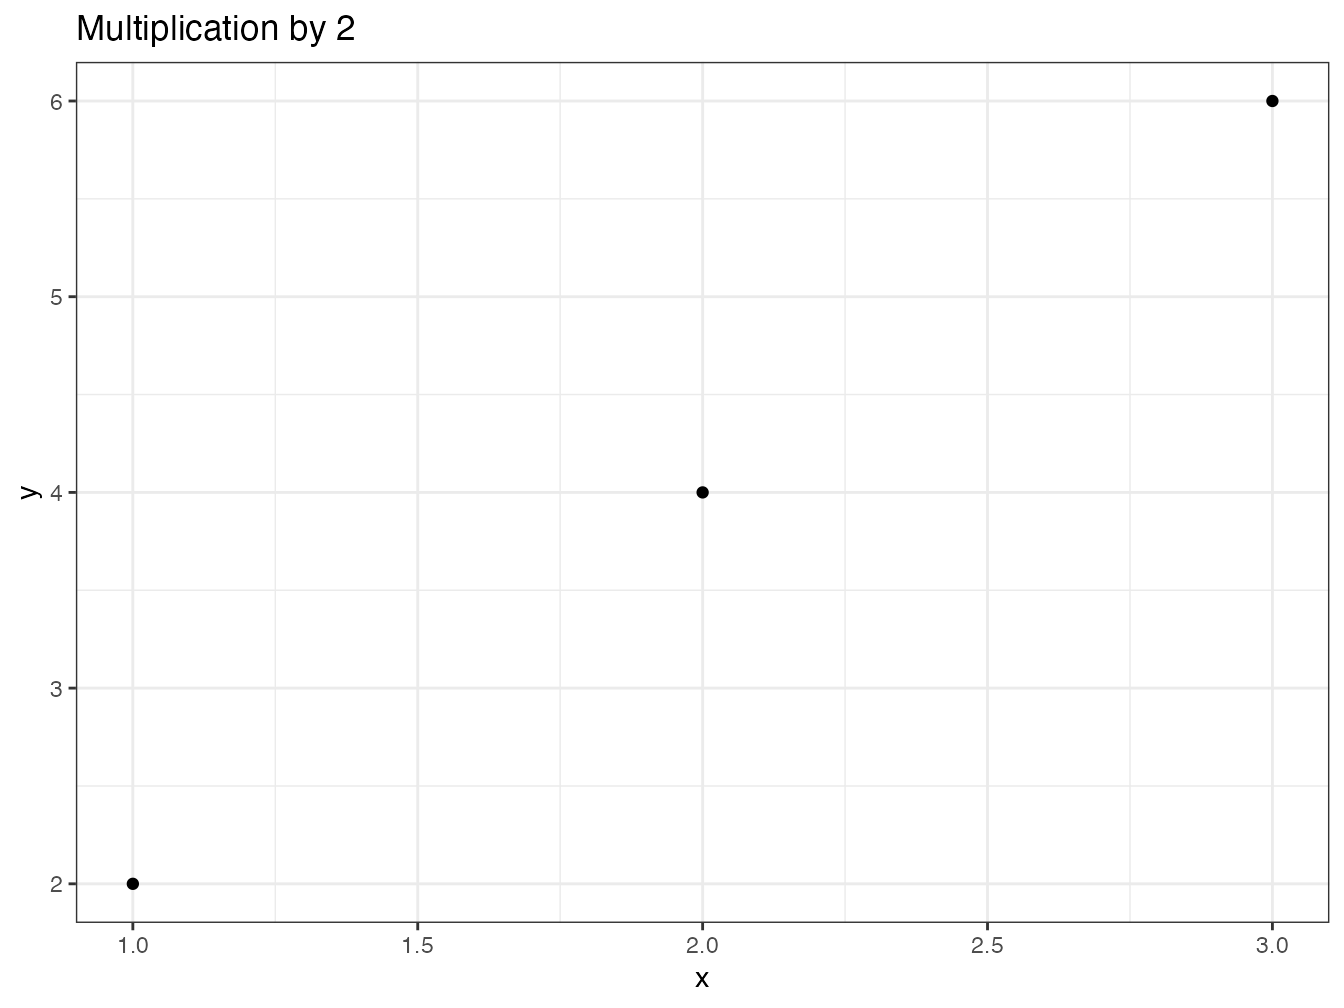
\includegraphics[width=0.8\linewidth]{WwR_files/figure-latex/plot.multiple-2} \end{center}

\normalsize

For technical reasons related to unconventional evaluation in the tidyverse, variable names used by \texttt{aes()} must be prefixed with \texttt{.data\$} in packages and \texttt{rlang::.data} must be imported.
Otherwise, the package check returns a note that the variables \texttt{x} and \texttt{y}, used by the arguments of \texttt{aes()} have not been declared and may not exist in the local environment (see section \ref{sec:environnements}).

\subsubsection{Documentation}\label{documentation}

Generic methods and functions that declare them must be documented like any other function.

Namespace management is a bit more complex:

\begin{itemize}
\tightlist
\item
  Generic methods must be exported:
\end{itemize}

\begin{verbatim}
#' @export
\end{verbatim}

\begin{itemize}
\tightlist
\item
  Functions derived from generic methods should not be exported but declared as methods, with the name of the generic method and the processed class.
  \textbf{roxygen2} requires that an export directive be added but does not enforce it (as it should) in the \texttt{NAMESPACE} file that is used by R:
\end{itemize}

\begin{verbatim}
#' @method plot multiple
#' @export
\end{verbatim}

\begin{itemize}
\tightlist
\item
  Since version 3 of \textbf{roxygen2}, the declaration \texttt{@method} is useless as long as the function name is unambiguously decomposable, like \texttt{plot.multiple}: \texttt{@export} is sufficient.
  If the derived function name has multiple dots, \textbf{roxygen2} may not automatically detect the generic and the object and \texttt{@method} must be maintained.
\item
  Functions derived from generic methods from another package need to import the generic method, unless it is provided by \textbf{base} (\texttt{print} is provided by \textbf{base} and is therefore not affected):
\end{itemize}

\begin{verbatim}
#' @importFrom graphics plot
#' @importFrom ggplot2 autoplot
\end{verbatim}

\begin{itemize}
\tightlist
\item
  The generics imported in this way must be re-exported by a directive to be placed for example just after the code of the derived function:
\end{itemize}

\begin{verbatim}
#' @export
graphics::plot

#' @export
ggplot2::autoplot
\end{verbatim}

\begin{itemize}
\tightlist
\item
  \textbf{roxygen2} automatically creates a help file \texttt{reexports.Rd} in which there is a link to the original documentation of the re-exported generics.
\end{itemize}

In \texttt{DESCRIPTION}, the original package for each generic must be listed in the \texttt{Imports:} directive:

\begin{verbatim}
Imports: ggplot2, graphics
\end{verbatim}

Last, importing functions from the tidyverse also requires some precautions:

\begin{itemize}
\tightlist
\item
  the \textbf{tidyverse} package is reserved for interactive use in R: there is no way to import it into \texttt{DESCRIPTION} because its dependencies may change and lead to unpredictable results.
  The \textbf{magrittr} package provides the pipes, mainly \texttt{\%\textgreater{}\%}.
  The \textbf{rlang} package provides the \texttt{.data} object shown below.
  They must be imported into \texttt{DESCRIPTION}.
\end{itemize}

\begin{verbatim}
Imports: magrittr, rlang, stats
\end{verbatim}

\begin{itemize}
\tightlist
\item
  Since it is not possible to prefix the \texttt{\%\textgreater{}\%} with the package name, the function must be imported using the delimiters provided for functions whose names contain special characters:
\end{itemize}

\scriptsize

\begin{Shaded}
\begin{Highlighting}[]
\CommentTok{\#\textquotesingle{} @importFrom magrittr \textasciigrave{}\%\textgreater{}\%\textasciigrave{}}
\end{Highlighting}
\end{Shaded}

\normalsize

\begin{itemize}
\tightlist
\item
  Functions in the tidyverse that use column names from tibbles or dataframes generate warnings at package check time because these names are confused with undefined variable names.
  To avoid this confusion, the \texttt{.data} object of the \textbf{rlang} package is helpful (for example in \texttt{aes()} seen above).
  It must be imported:
\end{itemize}

\scriptsize

\begin{Shaded}
\begin{Highlighting}[]
\CommentTok{\#\textquotesingle{} @importFrom rlang .data}
\end{Highlighting}
\end{Shaded}

\normalsize

Finally, the complete code is as follows:

\scriptsize

\begin{Shaded}
\begin{Highlighting}[]
\CommentTok{\#\textquotesingle{} Multiplication of a numeric vector}
\CommentTok{\#\textquotesingle{}}
\CommentTok{\#\textquotesingle{} @param number a numeric vector}
\CommentTok{\#\textquotesingle{} @param times a number to multiply}
\CommentTok{\#\textquotesingle{}}
\CommentTok{\#\textquotesingle{} @return an object of class \textasciigrave{}multiple\textasciigrave{}}
\CommentTok{\#\textquotesingle{} @export}
\CommentTok{\#\textquotesingle{}}
\CommentTok{\#\textquotesingle{} @examples}
\CommentTok{\#\textquotesingle{} multiple(1:2,3)}
\NormalTok{multiple }\OtherTok{\textless{}{-}} \ControlFlowTok{function}\NormalTok{(number, }\AttributeTok{times =} \DecValTok{1}\NormalTok{) \{}
  \CommentTok{\# Calculate the multiples}
\NormalTok{  y }\OtherTok{\textless{}{-}}\NormalTok{ number }\SpecialCharTok{*}\NormalTok{ times}
  \CommentTok{\# Save in a list}
\NormalTok{  result }\OtherTok{\textless{}{-}} \FunctionTok{list}\NormalTok{(}\AttributeTok{x =}\NormalTok{ number, }\AttributeTok{y =}\NormalTok{ y, }\AttributeTok{times =}\NormalTok{ times)}
  \CommentTok{\# Set the class}
  \FunctionTok{class}\NormalTok{(result) }\OtherTok{\textless{}{-}} \FunctionTok{c}\NormalTok{(}\StringTok{"multiple"}\NormalTok{, }\FunctionTok{class}\NormalTok{(result))}
  \FunctionTok{return}\NormalTok{(result)}
\NormalTok{\}}

\CommentTok{\#\textquotesingle{} Print objects of class multiple}
\CommentTok{\#\textquotesingle{}}
\CommentTok{\#\textquotesingle{} @param x an object of class \textasciigrave{}multiple\textasciigrave{}.}
\CommentTok{\#\textquotesingle{} @param ... further arguments passed to the generic method.}
\CommentTok{\#\textquotesingle{}}
\CommentTok{\#\textquotesingle{} @export}
\CommentTok{\#\textquotesingle{}}
\CommentTok{\#\textquotesingle{} @examples}
\CommentTok{\#\textquotesingle{} print(multiple(2,3))}
\NormalTok{print.multiple }\OtherTok{\textless{}{-}} \ControlFlowTok{function}\NormalTok{(x, ...) \{}
  \FunctionTok{print.default}\NormalTok{(x}\SpecialCharTok{$}\NormalTok{y)}
\NormalTok{\}}

\CommentTok{\#\textquotesingle{} Summarize objects of class multiple}
\CommentTok{\#\textquotesingle{}}
\CommentTok{\#\textquotesingle{} @param object an object of class \textasciigrave{}multiple\textasciigrave{}.}
\CommentTok{\#\textquotesingle{} @param ... further arguments passed to the generic method.}
\CommentTok{\#\textquotesingle{}}
\CommentTok{\#\textquotesingle{} @export}
\CommentTok{\#\textquotesingle{}}
\CommentTok{\#\textquotesingle{} @examples}
\CommentTok{\#\textquotesingle{} summary(multiple(2,3))}
\NormalTok{summary.multiple }\OtherTok{\textless{}{-}} \ControlFlowTok{function}\NormalTok{(object, ...) \{}
  \FunctionTok{print.default}\NormalTok{(object}\SpecialCharTok{$}\NormalTok{x)}
  \FunctionTok{cat}\NormalTok{(}\StringTok{"multiplied by"}\NormalTok{, object}\SpecialCharTok{$}\NormalTok{times, }\StringTok{"is:}\SpecialCharTok{\textbackslash{}n}\StringTok{"}\NormalTok{)}
  \FunctionTok{print.default}\NormalTok{(object}\SpecialCharTok{$}\NormalTok{y)}
\NormalTok{\}}

\CommentTok{\#\textquotesingle{} Plot objects of class multiple}
\CommentTok{\#\textquotesingle{}}
\CommentTok{\#\textquotesingle{} @param x a vector of numbers}
\CommentTok{\#\textquotesingle{} @param y a vector of multiplied numbers}
\CommentTok{\#\textquotesingle{} @param ... further arguments passed to the generic method.}
\CommentTok{\#\textquotesingle{}}
\CommentTok{\#\textquotesingle{} @importFrom graphics plot}
\CommentTok{\#\textquotesingle{} @export}
\CommentTok{\#\textquotesingle{}}
\CommentTok{\#\textquotesingle{} @examples}
\CommentTok{\#\textquotesingle{} plot(multiple(2,3))}
\NormalTok{plot.multiple }\OtherTok{\textless{}{-}} \ControlFlowTok{function}\NormalTok{(x, y, ...) \{}
  \FunctionTok{plot.default}\NormalTok{(}
    \AttributeTok{x =}\NormalTok{ x}\SpecialCharTok{$}\NormalTok{x, }
    \AttributeTok{y =}\NormalTok{ x}\SpecialCharTok{$}\NormalTok{y, }
    \AttributeTok{type =} \StringTok{"p"}\NormalTok{, }
    \AttributeTok{main =} \FunctionTok{paste}\NormalTok{(}\StringTok{"Multiplication by"}\NormalTok{, x}\SpecialCharTok{$}\NormalTok{times), }
\NormalTok{    ...}
\NormalTok{  )}
\NormalTok{\}}
\CommentTok{\#\textquotesingle{} @export}
\NormalTok{graphics}\SpecialCharTok{::}\NormalTok{plot}
\end{Highlighting}
\end{Shaded}

\begin{verbatim}
## function (x, y, ...) 
## UseMethod("plot")
## <bytecode: 0x12a9f2550>
## <environment: namespace:base>
\end{verbatim}

\begin{Shaded}
\begin{Highlighting}[]
\CommentTok{\#\textquotesingle{} autoplot}
\CommentTok{\#\textquotesingle{}}
\CommentTok{\#\textquotesingle{} ggplot of the \textasciigrave{}multiple\textasciigrave{} objects.}
\CommentTok{\#\textquotesingle{}}
\CommentTok{\#\textquotesingle{} @param object an object of class \textasciigrave{}multiple\textasciigrave{}.}
\CommentTok{\#\textquotesingle{} @param ... ignored.}
\CommentTok{\#\textquotesingle{}}
\CommentTok{\#\textquotesingle{} @return a \textasciigrave{}ggplot\textasciigrave{} object}
\CommentTok{\#\textquotesingle{} @importFrom ggplot2 autoplot}
\CommentTok{\#\textquotesingle{} @importFrom magrittr \textasciigrave{}\%\textgreater{}\%\textasciigrave{}}
\CommentTok{\#\textquotesingle{} @importFrom rlang .data}
\CommentTok{\#\textquotesingle{} @export}
\CommentTok{\#\textquotesingle{}}
\CommentTok{\#\textquotesingle{} @examples}
\CommentTok{\#\textquotesingle{} autoplot(multiple(2,3))}
\NormalTok{autoplot.multiple }\OtherTok{\textless{}{-}} \ControlFlowTok{function}\NormalTok{(object, ...) \{}
  \FunctionTok{data.frame}\NormalTok{(}\AttributeTok{x =}\NormalTok{ object}\SpecialCharTok{$}\NormalTok{x, }\AttributeTok{y =}\NormalTok{ object}\SpecialCharTok{$}\NormalTok{y) }\SpecialCharTok{\%\textgreater{}\%}
\NormalTok{    ggplot2}\SpecialCharTok{::}\FunctionTok{ggplot}\NormalTok{() }\SpecialCharTok{+}
\NormalTok{    ggplot2}\SpecialCharTok{::}\FunctionTok{geom\_point}\NormalTok{(ggplot2}\SpecialCharTok{::}\FunctionTok{aes}\NormalTok{(}\AttributeTok{x =}\NormalTok{ .data}\SpecialCharTok{$}\NormalTok{x, }\AttributeTok{y =}\NormalTok{ .data}\SpecialCharTok{$}\NormalTok{y)) }\SpecialCharTok{+}
\NormalTok{    ggplot2}\SpecialCharTok{::}\FunctionTok{labs}\NormalTok{(}\AttributeTok{title =} \FunctionTok{paste}\NormalTok{(}\StringTok{"Multiplication by"}\NormalTok{, object}\SpecialCharTok{$}\NormalTok{times))}
\NormalTok{\}}
\CommentTok{\#\textquotesingle{} @export}
\NormalTok{ggplot2}\SpecialCharTok{::}\NormalTok{autoplot}
\end{Highlighting}
\end{Shaded}

\begin{verbatim}
## function (object, ...) 
## {
##     UseMethod("autoplot")
## }
## <bytecode: 0x138774748>
## <environment: namespace:ggplot2>
\end{verbatim}

\normalsize

\subsection{C++ code}\label{c-code}

The use of C++ code has been seen in section \ref{sec:cpp}.
To integrate these functions in a package, the following rules must be respected:

\begin{itemize}
\tightlist
\item
  The \texttt{.cpp} files containing the code are placed in the \texttt{/src} folder of the project.
\item
  The code is commented for \textbf{roxygen2} in the same way as for R functions, but with the C language comment marker:
\end{itemize}

\scriptsize

\begin{Shaded}
\begin{Highlighting}[]
\PreprocessorTok{\#include }\ImportTok{\textless{}Rcpp.h\textgreater{}}
\KeywordTok{using} \KeywordTok{namespace}\NormalTok{ Rcpp}\OperatorTok{;}

\CommentTok{//\textquotesingle{} timesTwo}
\CommentTok{//\textquotesingle{}}
\CommentTok{//\textquotesingle{} Calculates the double of a value.}
\CommentTok{//\textquotesingle{}}
\CommentTok{//\textquotesingle{} @param x A numeric vector.}
\CommentTok{//\textquotesingle{} @export}
\CommentTok{// [[Rcpp::export]]}
\NormalTok{NumericVector timesTwo}\OperatorTok{(}\NormalTok{NumericVector x}\OperatorTok{)} \OperatorTok{\{}
  \ControlFlowTok{return}\NormalTok{ x }\OperatorTok{*} \DecValTok{2}\OperatorTok{;}
\OperatorTok{\}}
\end{Highlighting}
\end{Shaded}

\normalsize

\begin{itemize}
\tightlist
\item
  In \texttt{DESCRIPTION}, import the packages.
  \textbf{Rcpp}, and \textbf{RcppParallel} if parallelized code is used (delete its references otherwise), must be declared in \texttt{LinkingTo}:
\end{itemize}

\begin{verbatim}
Imports: Rcpp, RcppParallel
LinkingTo: Rcpp, RcppParallel
\end{verbatim}

\begin{itemize}
\tightlist
\item
  Comments for \textbf{roxygen2} should be added to \texttt{package.R} (\enquote{multiple} is the package name):
\end{itemize}

\scriptsize

\begin{Shaded}
\begin{Highlighting}[]
\CommentTok{\#\textquotesingle{} @importFrom Rcpp sourceCpp}
\CommentTok{\#\textquotesingle{} @importFrom RcppParallel RcppParallelLibs}
\CommentTok{\#\textquotesingle{} @useDynLib multiple, .registration = TRUE}
\end{Highlighting}
\end{Shaded}

\normalsize

\begin{itemize}
\tightlist
\item
  C++ working files are excluded from source control in \texttt{.gitignore}:
\end{itemize}

\begin{verbatim}
# C binaries
src/*.o
src/*.so
src/*.dll
\end{verbatim}

These changes are partly done automatically, for \textbf{Rcpp} only, by \textbf{usethis}, but manual insertion of the code is faster and more reliable: do not use this command.

\scriptsize

\begin{Shaded}
\begin{Highlighting}[]
\CommentTok{\# usethis::use\_rcpp()}
\end{Highlighting}
\end{Shaded}

\normalsize

Building the package will lead to compiling the code: Rtools are therefore essential.

\subsection{Tidy package}\label{tidy-package}

Any modern package should be tidyverse compatible, which requires little effort:

\begin{itemize}
\tightlist
\item
  To allow pipelines, the main argument of functions should be the first one.
\item
  Functions that transform data should accept a dataframe or tibble as the first argument and return an object of the same format.
\item
  Methods \texttt{plot()} should be doubled with methods \texttt{autoplot()} with the same arguments that produce the same graph with \textbf{ggplot2}.
\end{itemize}

\section{Bibliography}\label{bibliography-1}

The documentation of a package uses bibliographic references.
They can be managed automatically with \textbf{Rdpack} and \textbf{roxygen2}.
References used in R Markdown files (vignette, site produced by \textbf{pkgdown}) are not concerned.

\subsection{Preparation}\label{preparation}

Bibliographic references must be placed in a BibTeX file \texttt{REFERENCES.bib} placed in the \texttt{inst} folder.
This folder contains files that will be placed in the root of the package folder when it is installed.

Add the following line to \texttt{DESCRIPTION}:

\begin{verbatim}
RdMacros: Rdpack
\end{verbatim}

Also add the package \texttt{Rdpack} to the list of imported packages:

\begin{verbatim}
Imports: magrittr, stats, Rcpp, Rdpack
\end{verbatim}

Finally, import the \texttt{reprompt()} function from \textbf{Rdpack} by adding the following lines to the documentation for \textbf{roxygen2} in \texttt{package.R}:

\scriptsize

\begin{Shaded}
\begin{Highlighting}[]
\CommentTok{\#\textquotesingle{} @importFrom Rdpack reprompt}
\end{Highlighting}
\end{Shaded}

\normalsize

\subsection{Citations}\label{citations}

References are cited by the command \texttt{\textbackslash{}insertCite\{key\}\{package\}} in the documentation for \textbf{roxygen2}.
\texttt{package} is the name of the package in which the \texttt{REFERENCES.bib} file is to be searched: this will normally be the current package, but references to other packages are accessible, provided only that they use \textbf{Rdpack}.

\texttt{key} is the identifier of the reference in the file.
The following example\footnote{\textbf{divent} package on GitHub: \url{https://github.com/EricMarcon/divent/blob/master/R/package.R}} is from the documentation of the \textbf{divent} package hosted on GitHub, in its \texttt{.R} file:

\scriptsize

\begin{Shaded}
\begin{Highlighting}[]
\CommentTok{\#\textquotesingle{} divent}
\CommentTok{\#\textquotesingle{}}
\CommentTok{\#\textquotesingle{} Measures of Diversity and Entropy}
\CommentTok{\#\textquotesingle{} }
\CommentTok{\#\textquotesingle{} This package is a reboot of the **entropart** package \textbackslash{}insertCite\{Marcon2014c\}\{divent\}.}
\CommentTok{\#\textquotesingle{}}
\CommentTok{\#\textquotesingle{} @importFrom Rdpack reprompt}
\CommentTok{\#\textquotesingle{} }
\CommentTok{\#\textquotesingle{} @references}
\CommentTok{\#\textquotesingle{} \textbackslash{}insertAllCited\{\}}
\StringTok{"\_PACKAGE"}
\end{Highlighting}
\end{Shaded}

\begin{verbatim}
## [1] "_PACKAGE"
\end{verbatim}

\normalsize

The cited reference is in \texttt{inst/REFERENCES.bib}:

\begin{verbatim}
@Article{Marcon2014c,
  author  = {Marcon, Eric and Herault, Bruno},
  title   = {entropart, an R Package to Partition 
             Diversity},
  journal = {Journal of Statistical Software},
  year    = {2015},
  volume  = {67},
  number  = {8},
  pages   = {1--26},
}
\end{verbatim}

Citations are enclosed in parentheses.
To place the author's name outside the parenthesis, add the statement \texttt{;textual}:

\begin{verbatim}
\insertCite{Marcon2014c;textual}{divent}
\end{verbatim}

To cite several references (necessarily from the same package), separate them with commas.

At the end of the documentation of an object using citations, systematically add a list of references:

\scriptsize

\begin{Shaded}
\begin{Highlighting}[]
\CommentTok{\#\textquotesingle{} @references}
\CommentTok{\#\textquotesingle{} \textbackslash{}insertAllCited\{\}}
\end{Highlighting}
\end{Shaded}

\normalsize

\section{Data}\label{data}

Data can be embedded in a package, especially for the clarity of the examples.

The simplest method is to use \textbf{usethis}.
Create variables containing the data to be saved and then save them:

\scriptsize

\begin{Shaded}
\begin{Highlighting}[]
\NormalTok{seq1\_10 }\OtherTok{\textless{}{-}} \DecValTok{1}\SpecialCharTok{:}\DecValTok{10}
\NormalTok{seq1\_100 }\OtherTok{\textless{}{-}} \DecValTok{1}\SpecialCharTok{:}\DecValTok{100}
\NormalTok{usethis}\SpecialCharTok{::}\FunctionTok{use\_data}\NormalTok{(seq1\_10, seq1\_100)}
\end{Highlighting}
\end{Shaded}

\normalsize

An \texttt{.rda} file is created in the \texttt{data} folder for each variable created.
With the \texttt{LazyData} option enabled in \texttt{DESCRIPTION}, variables will be available as soon as the package is loaded, but will not actually be loaded into memory until after they are used for the first time.

Each variable must be documented in the \texttt{package.R} file:

\scriptsize

\begin{Shaded}
\begin{Highlighting}[]
\CommentTok{\#\textquotesingle{} seq1\_10}
\CommentTok{\#\textquotesingle{}}
\CommentTok{\#\textquotesingle{} A sequence of numbers from 1 to 10}
\CommentTok{\#\textquotesingle{}}
\CommentTok{\#\textquotesingle{} @format A numeric vector.}
\CommentTok{\#\textquotesingle{} @source Values computed by the R software, }
\CommentTok{\#\textquotesingle{}   \textbackslash{}url\{https://www.r{-}project.org/\}}
\StringTok{"seq1\_10"}
\end{Highlighting}
\end{Shaded}

\normalsize

The name of the variable is given in quotes after the comment block (instead of the R code of a function).
\texttt{@format} describes the format of the data and \texttt{@source} is used to indicate its source.

\section{Unit tests}\label{unit-tests}

Ideally, all code included in a package should be tested in multiple ways:

\begin{itemize}
\tightlist
\item
  Against syntax errors: R's checking procedures handle this quite well.
\item
  To check the conformity of the computation results to the expected values.
\item
  Against the occurrence of errors if users do not use the code as the developer intended (incorrect arguments passed to functions, inadequate data\ldots).
\end{itemize}

Unit tests are used for the last two objectives.
They are based on \textbf{testthat} to be integrated in the package:

\scriptsize

\begin{Shaded}
\begin{Highlighting}[]
\NormalTok{usethis}\SpecialCharTok{::}\FunctionTok{use\_testthat}\NormalTok{()}
\end{Highlighting}
\end{Shaded}

\normalsize

\scriptsize

\normalsize

The tests must be added as \texttt{.R} files whose names must begin with \texttt{test\textquotesingle{}\ in\ the}tests/testthat` folder.

Each test (so the content of each file) starts with its context, i.e.~a set of tests. For example, in a file \texttt{test\_double.R}:

\scriptsize

\begin{Shaded}
\begin{Highlighting}[]
\FunctionTok{context}\NormalTok{(}\StringTok{"function double"}\NormalTok{)}
\end{Highlighting}
\end{Shaded}

\normalsize

The tests are contained in files that group them by topic, for example \texttt{test\_double.R}.
The name of each test is passed as an argument to the function \texttt{test\_that()}:

\scriptsize

\begin{Shaded}
\begin{Highlighting}[]
\FunctionTok{test\_that}\NormalTok{(}\StringTok{"Double values are correct"}\NormalTok{, \{}
  \FunctionTok{skip\_on\_cran}\NormalTok{()}

\NormalTok{  x }\OtherTok{\textless{}{-}} \DecValTok{1}\SpecialCharTok{:}\DecValTok{2}

  \CommentTok{\# 2 x 2 should be 4}
  \FunctionTok{expect\_equal}\NormalTok{(}\FunctionTok{double}\NormalTok{(x), }\FunctionTok{c}\NormalTok{(}\DecValTok{2}\NormalTok{, }\DecValTok{4}\NormalTok{))}
  \CommentTok{\# The result should be a number (type = "double")}
  \FunctionTok{expect\_type}\NormalTok{(}\FunctionTok{double}\NormalTok{(x), }\StringTok{"double"}\NormalTok{)}
  \CommentTok{\# Error management}
  \FunctionTok{expect\_error}\NormalTok{(}\FunctionTok{double}\NormalTok{(}\StringTok{"a"}\NormalTok{))}
\NormalTok{\})}
\end{Highlighting}
\end{Shaded}

\begin{verbatim}
## Test passed
\end{verbatim}

\normalsize

All functions starting with \texttt{expect} allow to compare their first argument to a result: in the above example, the result of \texttt{double(1:2)} must be \texttt{2\ 4} and the type of this vector must be double precision real.
The last test checks whether a string passed as an argument generates an error, which is not optimal: if the package handled the error, the returned message could be tested.

The \texttt{skip\_on\_cran()} command, to be used systematically, avoids running the tests on CRAN when the package is dropped there: CRAN has limited resources and strictly limits the time for checking packages on its platform.
The tests will therefore have to be run on GitHub, thanks to continuous integration, see section \ref{sec:package-ci5}.

The tests can be launched by the \enquote{More \textgreater{} Test package} menu of the \emph{Build} window or by the \texttt{devtools::test()} command.

It is advisable to write the tests as soon as a function of the package is stabilized.

\section{.gitignore file}\label{gitignore-file}

The \texttt{.gitignore} file obtained at this stage is incomplete.
It can be replaced by this one:

\begin{verbatim}
# History files
.Rhistory
.Rapp.history
# Session Data files
.RData
# Example code in package build process
*-Ex.R
# Output files from R CMD build
/*.tar.gz
# Output files from R CMD check
/*.Rcheck/
# RStudio files
.Rproj.user/
.Rprofile
# knitr and R markdown default cache directories
*_cache/
/cache/
# Temporary files created by R markdown
*.utf8.md
*.knit.md
# C binaries
src/*.o
src/*.so
src/*.dll
/src-i386/
/src-x64/
# uncomment if pkgdown is run by CI
# docs/
\end{verbatim}

The last line is for the \texttt{docs/} folder, which receives the web site produced by \textbf{pkgdown}.
It is commented out as long as the production of the site is done locally, but uncommented if it is entrusted to GitHub Actions (see next section).

\section{Continuous integration}\label{sec:package-ci5}

A package check must be done at each step of the development, which consumes a considerable amount of time.
It can be automated very easily with the GitHub Actions service, triggered at each modification of the repository on GitHub.
The analysis of the code coverage by tests (which parts of the code are tested or not) will be added.

GitHub is also able to rebuild the package documentation with \textbf{pkgdown}, another resource-consuming operation, after the tests have passed.

Section \ref{sec:package-ci6} details how to do this.

\section{CRAN}\label{sec:package-cran}

Packages with an audience beyond the author's circle can be uploaded to CRAN.
The rules to respect on CRAN are numerous\footnote{\url{https://cran.r-project.org/web/packages/policies.html}}. They are checked by the \texttt{R\ CMD\ check} command with the \texttt{-\/-\ as.cran} option.
The check must not return any errors, warnings, or notes before submitting the package.

\subsection{Testing the package}\label{testing-the-package}

Verification of the package by GitHub as part of continuous integration is not sufficient.
The package must be tested on the development version of R.
The \emph{R-hub builder}\footnote{\url{https://builder.r-hub.io/}} site allows to do it easily.

The package, which must not be a development version (limited to three numbers, see section \ref{sec:package-description}), must be built in source format: in the \emph{Build} window of RStudio, click on \enquote{More \textgreater{} Build Source Package}.
On the \emph{R-hub builder} site, click on \enquote{Advanced}, select the package source file and the test platform: \emph{Debian Linux, R-devel, GCC}.

The \textbf{rhub} package allows you to use the same verification platform as the \emph{R-hub builder} site from RStudio.
The first step is to validate your email address with the \texttt{validate\_email()} command.
Then, just call the \texttt{check\_for\_cran()} function to run a full verification.

\subsection{Submission}\label{submission}

When the package is ready, submission to CRAN is done through the dedicated web site\footnote{\url{https://xmpalantir.wu.ac.at/cransubmit/}}.

In case of rejection, process the requests and resubmit after incrementing the version number.

\subsection{Maintenance}\label{maintenance}

Requests for corrections are sent by CRAN from time to time, especially when the version of R changes.
The email address of the package maintainer must remain valid and the requests must be processed quickly.
Otherwise, the package is archived.

New versions of the package are submitted in the same way as the first one.

\chapter{Continuous integration}\label{chap-ci}

\toc{1}

Continuous integration is the process of assigning an external service to verify a package, produce Markdown documents for web pages in a GitHub repository, or completely knit a website from code.

All of these tasks can be done locally on the desktop but are time consuming and may not be repeated with each update.
In the context of continuous integration, they are systematically performed, in a transparent way for the user.
In case of failure, an alert message is sent.

The implementation of continuous integration is justified for heavy projects, with regular updates.
rather than for projects containing a simple Markdown document that is rarely modified.

\section{Tools}\label{tools}

\subsection{GitHub Actions}\label{github-actions}

The most frequently used tool for R projects filed on GitHub was \emph{Travis CI}\footnote{\url{https://travis-ci.org/}} but the service became fee-based in 2021.

GitHub Shares is a good replacement for Travis.
This service is integrated with GitHub.

\subsection{Codecov}\label{codecov}

To evaluate the code coverage rate of R packages, i.e.~the proportion of code tested in some way (examples, unit tests, vignette), the \emph{Codecov}\footnote{\url{https://codecov.io/}} service integrates perfectly with GitHub.

You need to open an account, preferably by authenticating through GitHub.

\subsection{GitHub Pages}\label{github-pages}

GitHub web pages can be hosted in the \texttt{docs} directory of the master branch of the project: this is the solution chosen when they are produced on the workstation.

If they are produced by continuous integration, they will be hosted in a dedicated branch called \texttt{gh-pages}.

\section{Principles}\label{principles}

The production of a document is treated as an example.
The objective is to have GitHub knit a Markdown project.
This practice is appropriate for book projects, which require a lot of resources for their construction.
In this type of project, the code is knit by \textbf{knitr} to produce several documents, typically in HTML and PDF formats, accessible on GitHub pages.
When documents are produced locally, they are placed in the \texttt{docs} folder and pushed to GitHub.

In order for GitHub to do this, a few settings are required.

\subsection{Getting a personal access token}\label{getting-a-personal-access-token}

To write to GitHub, the continuous integration service will have to authenticate with a Personal Access Token (PAT) whose creation is described in section \ref{sec:pat}.

Generate a new token, describe it as \enquote{GitHub Actions} and give it the following authorizations:

\begin{itemize}
\tightlist
\item
  \enquote{repo}, i.e.~modify \emph{all} repositories (it is not possible to limit access to a particular repository).
\item
  \enquote{workflow}, i.e.~run continuous integration scripts.
\end{itemize}

\subsection{Project secrets}\label{sec:secrets-ci}

On GitHub, display the project settings and select \enquote{Secrets}.
The \enquote{New Repository Secret} button allows you to store variables used in GitHub Actions scripts (publicly visible) without exposing their value.
The personal access token is essential for GitHub Actions to write their production in the project.
Create a secret named \enquote{GH\_PAT} and enter the previously saved token value.
After clicking on \enquote{Add Secret}, the token cannot be read anymore.

To allow sending success or failure messages without exposing your email address, create a secret named \enquote{EMAIL} which contains it.

\subsection{Activation of the repository on CodeCov}\label{activation-of-the-repository-on-codecov}

The analysis of the code coverage of packages is useful to detect untested code portions.
On the other hand, the analysis of the coverage of document projects is not useful.

To activate a repository, you need to authenticate on the CodeCov website with your GitHub account.
The list of repositories is displayed and can be updated.
If the repositories to be processed are hosted by an organization, for example the repositories of a GitHub classroom, you have to update the list of organizations by following the instructions (a link allows you to quickly modify the GitHub options to authorize Codecov to read the data of an organization) and update the list of repositories again.
Finally, when the repository you are looking for is visible, you have to activate it.
Ignore Codecov's token system.

\subsection{Scripting GitHub actions}\label{scripting-github-actions}

A GitHub workflow is a succession of jobs with steps.
A workflow is triggered by an event, usually every \emph{push} of the project, but also at regular intervals (\emph{cron}).

Typically, the workflows created here contain two jobs: the first one installs R and the necessary components and executes R scripts (which constitute its successive steps); the second one publishes the obtained files in GitHub pages.

The workflows are configured in a YAML file placed in the \texttt{.github/workflows/} folder of the project.
The different parts of the script are presented below.
The full script is that of this document, accessible on GitHub\footnote{\url{https://github.com/EricMarcon/WorkingWithR/blob/master/.github/workflows/bookdown.yml}}.

\subsubsection{Trigger}\label{sec:declenchement}

The action is triggered whenever updates are pushed to GitHub:

\begin{verbatim}
on:
  push:
     branches:
       - master
\end{verbatim}

The branch taken into account is \emph{master} (to be replaced by \emph{main} if necessary).

To trigger the action periodically, use the syntax of cron (the Unix job scheduling system):

\begin{verbatim}
on:
  schedule:
    - cron: '0 22 * * 0' # every sunday at 22:00
\end{verbatim}

The successive values are for minutes, hours, day (day of the month), month and day of the week (0 for Sunday to 6 for Saturday).
The \texttt{*} allow to ignore a value.

The \texttt{push} and \texttt{schedule} entries can be used together:

\begin{verbatim}
on:
  push:
     branches:
       - master
  schedule:
    - cron: '0 22 * * 0'
\end{verbatim}

Currently, scheduling is only taken into account in the \emph{master} branch.

\subsubsection{Workflow name}\label{workflow-name}

The name of the workflow is free.
It will be displayed by the badge that will be added to the project's \texttt{README.md} file (see section \ref{sec:ci-badges}).

\begin{verbatim}
name: bookdown
\end{verbatim}

\subsubsection{First job}\label{first-job}

The jobs are described in the \texttt{jobs} section.
\texttt{renderbook} is the name of the first job: it is free.
Here, the main action will be to produce a bookdown with the \texttt{render\_book()} function, hence the name.

\begin{verbatim}
jobs:
  renderbook:
    runs-on: macOS-latest
\end{verbatim}

The \texttt{runs-on} statement describes the operating system on which the job should run.
The possible choices are Windows, Ubuntu or MacOS\footnote{\url{https://docs.github.com/en/free-pro-team@latest/actions/reference/workflow-syntax-for-github-actions\#jobsjob_idruns-on}}.
Continuous integration of R on GitHub usually uses MacOS which has the advantage of using compiled R packages so much simpler (some packages require libraries outside of R for their compilation) and quicker to install, while allowing the use of scripts.

\subsubsection{First steps}\label{first-steps}

The steps are described in the \texttt{steps} section.

\begin{verbatim}
    steps:
      - name: Checkout repo
        uses: actions/checkout@v4
      - name: Setup R
        uses: r-lib/actions/setup-r@v2
      - name: Install pandoc
        run: |
          brew install pandoc
\end{verbatim}

Each step is described by its name (free) and what it does.

The strength of GitHub Actions is to allow the use of \emph{actions} written by other people and stored in a public GitHub project.
An action is a script with metadata describing its use.
Its development is accompanied by successive version numbers.
An action is called by the statement \texttt{uses:}, the GitHub project that contains it and its version.

In their respective GitHub project, actions exist in their development version (\texttt{@master}) and in step versions (\emph{release}) accessible by their number (\texttt{@v1}).
These stage versions are preferable because they are stable.

General actions are made available by GitHub in the GitHub Actions organization\footnote{\url{https://github.com/actions/}}.
The \enquote{actions/checkout} action is used to get into the main branch of the project processed by the workflow: it is usually the first step of all workflows.

The next action is the installation of R, provided by the \emph{R infrastructure} organization\footnote{\url{https://github.com/r-lib/}}.

The installation of pandoc (software external to R but necessary for R Markdown) can be done by a command executed by MacOS.
It is called by \texttt{run:} and can contain several lines (hence the \texttt{\textbar{}}).
This script depends on the operating system: \texttt{brew} is the package manager of MacOS.
To avoid system specifics, it is better to use an action:

\begin{verbatim}
      - name: Install pandoc
        uses: r-lib/actions/setup-pandoc@v2
\end{verbatim}

It is often possible to choose between calling an action or writing the corresponding code.
The choice made here is to favour actions for everything to do with the system, such as installing software, but to use scripts for R commands, such as checking packages.
The aim is to control the R code precisely and limit dependencies on additional packages.
The opposite strategy is developed in \textcite{Wickham2023} which relies entirely on actions to perform R tasks.

\subsubsection{Packages}\label{sec:packages-ci}

This step uses \texttt{Rscript} as its command environment, which allows it to execute R commands directly.

\begin{verbatim}
      - name: Install packages
        env:
          GITHUB_PAT: ${{ secrets.GH_PAT }}
        run: |
          options(pkgType = "binary")
          options(install.packages.check.source = "no")
          install.packages(c("remotes", "bookdown", "formatR", "tinytex"))
          tinytex::install_tinytex(bundle = "TinyTeX")
          remotes::install_deps(dependencies = TRUE)
        shell: Rscript {0}
\end{verbatim}

The packages used to produce the document are listed:

\begin{itemize}
\tightlist
\item
  \textbf{remotes} for its \texttt{install\_deps()} function.
\item
  \textbf{bookdown} for knitting.
\item
  \textbf{formatR} for formatting code snippets (\texttt{tidy=TRUE}).
\item
  \textbf{tinytex} to have a LaTeX distribution.
\end{itemize}

The other packages, those used by the project, are read in the \texttt{DESCRIPTION} file by the \texttt{install\_deps()} function.

On MacOS, packages are installed by default in binary version, but from their source code if it is more recent.
The creation of binary packages takes a few days at CRAN: this situation is not rare.
Packages containing only R code or C++ code without reference to external libraries can be installed without problems.
On the other hand, if the package requires libraries external to R or a compilation of Fortran code, the installation fails.
It would therefore be necessary to install the necessary libraries (and possibly a Fortran compiler) for all the packages on which the project depends: this solution is not realistic because it implies an inventory of all the dependencies, which may change, and a large number of time-consuming and useless installations most of the time, when the binary packages are up to date.
A better solution is to force the installation of binary packages even if the source code is newer: this is the purpose of the two R options defined before calling \texttt{install.packages()}.

Finally, the secret \texttt{GH\_PAT} is passed to R in an environment variable, \texttt{GITHUB\_PAT}, necessary to install packages from their source code on GitHub.
GitHub limits the rate of anonymous access for all GitHub actions (all accounts) and may reject the request: in practice, using \texttt{install\_github()} in a GitHub action is only possible with this environment variable.

\subsubsection{Knitting}\label{knitting}

The production of the document is started by an R command.

\begin{verbatim}
      - name: Render pdf book
        run: |
          bookdown::render_book("index.Rmd", "bookdown::pdf_book")
        shell: Rscript {0}
      - name: Render gitbook
        run: |
          bookdown::render_book("index.Rmd", "bookdown::gitbook")
        shell: Rscript {0}
\end{verbatim}

The parameters declared in \texttt{\_output.yml} are used.

The PDF file must be produced before the GitBook format in order for its download link to be added to the menu bar of the GitBook site.
On the other hand, R must be closed and reopened between the two renderings otherwise the tables are not created correctly in GitBook\footnote{\url{https://stackoverflow.com/questions/46080853/why-does-rendering-a-pdf-from-rmarkdown-require-closing-rstudio-between-renders/46083308\#46083308}}.
The two steps should not be combined into one.

\subsubsection{Backup}\label{backup}

The result of the knitting, placed in the \texttt{docs} folder of the virtual machine in charge of continuous integration, must be preserved so that the next job can use it.

The last step of the production job uses the \texttt{upload-artifact} action for this.

\begin{verbatim}
      - name: Upload artifact
        uses: actions/upload-artifact@v4
        with:
          name: _book
          path: docs/
\end{verbatim}

The content of \texttt{docs} is saved as an \emph{artifact} named ``\_book''.
Artifacts are publicly visible on the GitHub Project Actions page.

After its last step, the virtual machine is destroyed.

\subsubsection{Publication}\label{publication}

Publishing the artifact to the \texttt{gh-pages} branch of the project requires another job.

\begin{verbatim}
  deploy:
    runs-on: ubuntu-latest
    needs: renderbook
    permissions:
      contents: write
    steps:
      - name: Download artifact
        uses: actions/download-artifact@v4
        with:
          # Artifact name
          name: _book
          # Destination path
          path: docs
      - name: Deploy to GitHub Pages
        uses: Cecilapp/GitHub-Pages-deploy@v3
        env:
          GITHUB_TOKEN: ${{ secrets.GITHUB_TOKEN }}
        with:
          email: ${{ secrets.EMAIL }}
          build_dir: docs
          jekyll: no
\end{verbatim}

The job is named \enquote{deploy} (the name is free).
It runs on a virtual machine on Ubuntu.
It can only be launched if the \enquote{renderbook} job has succeeded.
Its steps are the following:

\begin{itemize}
\tightlist
\item
  \emph{Download artifact}: Restore the \texttt{docs} folder;
\item
  \emph{Deploy to GitHub Pages}: copy the \texttt{docs} folder to the \texttt{gh-pages} branch.
\end{itemize}

This last step uses the \texttt{GitHub-Pages-deploy} action provided by the \emph{Cecilapp} organization.
It uses an environment variable, \texttt{GITHUB\_TOKEN}, to authenticate and parameters:

\begin{itemize}
\tightlist
\item
  \emph{email}: the email address to which the run report is sent.
  To avoid exposing the address publicly, it has been stored in a project secret.
\item
  \emph{buid\_dir}: the directory to publish.
\item
  \emph{jekyll:no} to create an empty file named \texttt{.nojekyll} that tells GitHub pages not to try to treat their content as a Jekyll website.
\end{itemize}

GITHUB\_TOKEN\texttt{is\ an\ authentication\ token\ provided\ by\ Github\ Actions\ for\ the\ execution\ of\ this\ script.\ Its\ rights\ are\ assigned\ in\ the\ script\ by\ the}permission` entry: here, the right to write content to the project.

\subsection{Confidential data in a public repository}\label{sec:confidentielCI}

If the project contains confidential data (section \ref{sec:confidential}), GitHub Actions must use the project's private key to extract it from their vault.

The private key must be stored in a project secret, named \enquote{RSA}.
The next step, to be inserted before the knitting step, writes the key to a file for the project code to access.

\begin{verbatim}
      - name: Private key
        run: |
          cat("${{ secrets.rsa }}", file="<RepoID>.rsa"
        shell: Rscript {0}
\end{verbatim}

\section{Script templates}\label{script-templates}

Script templates for all types of projects are presented here.

The \texttt{gh-pages} branch is created automatically by the scripts.
Check after the first execution that GitHub pages are enabled on this branch (section \ref{sec:github-pages}).
Then delete the \texttt{docs} folder if it existed, push the modification on GitHub and finally add the following line to the \texttt{.gitignore} file to be able to knit the projects locally without disturbing GitHub:

\begin{verbatim}
docs/
\end{verbatim}

\subsection{memoiR}\label{sec:memoiR-ci}

The \texttt{build\_ghworkflow()} function of the \textbf{memoiR} package automatically creates the scripts needed to produce the package's templates.
The script is always named \texttt{memoir.yml}.

These scripts do not need a \texttt{DESCRIPTION} file for the installation of the dependencies but each document must contain in its parameter code (\texttt{Options}) the list of all packages needed for its knitting (stored in the \texttt{Packages} variable).

They all require the same preparation: the \texttt{GH\_PAT} and \texttt{EMAIL} secrets must be registered in the GitHub project (section \ref{sec:secrets-ci}).

\subsubsection{Book or thesis}\label{sec:bookdown-ci}

The workflow is called \texttt{rmarkdown}; its production job is \texttt{render}.

\begin{verbatim}
on:
  push:
   branches:
     - master

name: rmarkdown

jobs:
  render:
    runs-on: macOS-latest
    steps:
      - name: Checkout repo
        uses: actions/checkout@v4
      - name: Setup R
        uses: r-lib/actions/setup-r@v2
      - name: Install pandoc
        uses: r-lib/actions/setup-pandoc@v2
      - name: Install dependencies
        run: |
          options(pkgType = "binary")
          options(install.packages.check.source = "no")
          install.packages(
            c("distill", "downlit", "memoiR", "rmdformats", "tinytex")
          )
          tinytex::install_tinytex(bundle = "TinyTeX")
        shell: Rscript {0}
      - name: Render pdf book
        run: |
          bookdown::render_book("index.Rmd", "bookdown::pdf_book")
        shell: Rscript {0}
      - name: Render gitbook
        run: |
          bookdown::render_book("index.Rmd", "bookdown::gitbook")
        shell: Rscript {0}
      - name: Upload artifact
        uses: actions/upload-artifact@v4
        with:
          name: ghpages
          path: docs
  deploy:
    runs-on: ubuntu-latest
    needs: render
    permissions:
      contents: write
    steps:
      - name: Download artifact
        uses: actions/download-artifact@v4
        with:
          name: ghpages
          path: docs
      - name: Deploy to GitHub Pages
        uses: Cecilapp/GitHub-Pages-deploy@v3
        env:
          GITHUB_TOKEN: ${{ secrets.GITHUB_TOKEN }}
        with:
          email: ${{ secrets.EMAIL }}
          build_dir: docs
          jekyll: no
\end{verbatim}

\subsubsection{Articles or slideshows}\label{articles-or-slideshows}

The workflow is called \texttt{rmarkdown}; its production job is \texttt{render}.

\begin{verbatim}
on:
  push:
   branches:
     - master

name: rmarkdown

jobs:
  render:
    runs-on: macOS-latest
    steps:
      - name: Checkout repo
        uses: actions/checkout@v4
      - name: Setup R
        uses: r-lib/actions/setup-r@v2
      - name: Install pandoc
        uses: r-lib/actions/setup-pandoc@v2
      - name: Install dependencies
        run: |
          options(pkgType = "binary")
          options(install.packages.check.source = "no")
          install.packages(c("memoiR", "rmdformats", "tinytex"))
          tinytex::install_tinytex()
        shell: Rscript {0}
      - name: Render Rmarkdown files
        run: |
          RMD_PATH=($(ls | grep "[.]Rmd$"))
          Rscript -e 'for (file in commandArgs(TRUE)) |>
              rmarkdown::render(file, "all")' ${RMD_PATH[*]}
          Rscript -e 'memoiR::build_githubpages(bundle = "TinyTeX")'
      - name: Upload artifact
        uses: actions/upload-artifact@v4
        with:
          name: ghpages
          path: docs
  deploy:
    runs-on: ubuntu-latest
    needs: render
    permissions:
      contents: write
    steps:
      - name: Download artifact
        uses: actions/download-artifact@v4
        with:
          name: ghpages
          path: docs
      - name: Deploy to GitHub Pages
        uses: Cecilapp/GitHub-Pages-deploy@v3
        env:
          GITHUB_TOKEN: ${{ secrets.GITHUB_TOKEN }}
        with:
          email: ${{ secrets.EMAIL }}
          build_dir: docs
          jekyll: yes
\end{verbatim}

The knitting stage uses a script to list all the \texttt{.Rmd} files, process them (all the output formats listed in their yaml header are produced).
The \texttt{build\_githubpages()} function (see section \ref{sec:memo}) places the results in \texttt{docs}.

The deployment job tells GitHub pages to use Jekyll, i.e.~to use the \texttt{README.md} file as the home page.

\subsubsection{Localization}\label{localization}

If the knitting step needs to change the language used by R, for example to correctly display the production date of documents, it can be changed like this:

\begin{verbatim}
      - name: Render Rmarkdown files
        run: |
          Sys.setlocale("LC_TIME", "fr_FR")
          lapply(list.files(pattern="*.Rmd"), 
                            function(file) rmarkdown::render(file, "all"))
          memoiR::build_githubpages()
        shell: Rscript {0}
\end{verbatim}

The selection of files is done by an R script, which includes a localization command, here in French.

This step can be completed by selecting a GitHub Pages theme so that the home page contains a link to the code:

\begin{verbatim}
        run: |
          echo 'theme: jekyll-theme-slate' > docs/_config.yml
\end{verbatim}

The theme here is \enquote{Slate}, one of the choices offered by the GitHub pages.

\subsubsection{Debugging}\label{debugging}

It can happen that the compilation of the \texttt{.tex} file to produce the PDF file fails, although knitting in HTML does not generate an error.
The LaTeX compiler is indeed more demanding than pandoc (which produces the HTML file).

The first check consists in knitting the problematic document into PDF locally, on your workstation, with \textbf{tinytex}.
The LaTeX packages must be updated to be the same as those used by the GitHub actions: to do this, run:

\scriptsize

\begin{Shaded}
\begin{Highlighting}[]
\NormalTok{tinytex}\SpecialCharTok{::}\FunctionTok{tlmgr\_update}\NormalTok{()}
\end{Highlighting}
\end{Shaded}

\normalsize

If the compilation works locally but not on Github, you have to inspect the \texttt{.log} file which records all the events generated by the compiler, but this file is not kept after the failure of GitHub Actions.
So you have to modify the script to copy the file in \texttt{docs} and then save the result despite the error.

The \enquote{Upload artifact} step is modified to run despite the failure of the previous step by adding the line \texttt{if:}:

\begin{verbatim}
      - name: Upload artifact
        if: always()
        uses: actions/upload-artifact@v4
        with:
          name: _book
          path: docs/
\end{verbatim}

A step is added before \enquote{Upload artifact} to copy the result of the knitting and the \texttt{.log} file:

\begin{verbatim}
      - name: Move files to docs
        if: always()
        run: |
          Rscript -e 'memoiR::build_githubpages()'
          cp *.log docs
\end{verbatim}

After the action fails, the saved artifact can be downloaded from GitHub: it is on the action summary page.
It is a compressed file that contains the whole \texttt{docs} folder.

\subsection{Blogdown website}\label{sec:blogdown-ci}

The file called \texttt{blogdown.yml} is very similar.
The name of the workflow is \texttt{blogdown} and the name of the production job is \texttt{buildsite}.

\begin{verbatim}
on:
  push:
     branches:
       - master
  schedule:
    - cron: '0 22 * * 0'

name: blogdown

jobs:
  buildsite:
    runs-on: macOS-latest
    steps:
      - name: Checkout repo
        uses: actions/checkout@v4
      - name: Setup R
        uses: r-lib/actions/setup-r@v2
      - name: Install pandoc
        uses: r-lib/actions/setup-pandoc@v2
      - name: Install packages
        run: |
          options(pkgType = "binary")
          options(install.packages.check.source = "no")
          install.packages(c("remotes", "blogdown", "formatR"))
          remotes::install_deps(dependencies = TRUE)
        shell: Rscript {0}
      - name: Build website
        run: |
          blogdown::install_hugo(force = TRUE)
          blogdown::build_site(local = TRUE, build_rmd = TRUE)
        shell: Rscript {0}
      - name: Upload artifact
        uses: actions/upload-artifact@v4
        with:
          name: _website
          path: public/
  deploy:
    runs-on: ubuntu-latest
    needs: buildsite
    permissions:
      contents: write
    steps:
      - name: Download artifact
        uses: actions/download-artifact@v4
        with:
          # Artifact name
          name: _website
          # Destination path
          path: public
      - name: Deploy to GitHub Pages
        uses: Cecilapp/GitHub-Pages-deploy@v3
        env:
          GITHUB_TOKEN: ${{ secrets.GITHUB_TOKEN }}
        with:
          build_dir: public
          email: ${{ secrets.EMAIL }}
          jekyll: no
\end{verbatim}

The \texttt{Build\ website} step uses the \textbf{blogdown} package to install Hugo (the website generator) and then build the website.

If the website uses online data that warrants periodic updating, GitHub Actions can be run daily, weekly or monthly in addition to the rebuilds triggered by a repository change (see section \ref{sec:declenchement}).
Here, the site is rebuilt every Sunday at 10pm.

Example: the page that displays the bibliometrics of the author's website\footnote{\url{https://EricMarcon.github.io/fr/publication/}} queries Google Scholar to display the citations of the publications.
The site is updated weekly to keep the statistics current.

\subsection{R Packages}\label{sec:package-ci6}

An optimal script for checking a package is as follows:

\begin{verbatim}
on:
  push:
    branches:
      - master

name: R-CMD-check

jobs:
  R-CMD-check:
    runs-on: macOS-latest
    steps:
      - name: Pull the repository
        uses: actions/checkout@v4
      - name: Install R
        uses: r-lib/actions/setup-r@v2
      - name: Install pandoc
        uses: r-lib/actions/setup-pandoc@v2
      - name: Install R packages
        run: |
          options(pkgType = "binary")
          options(install.packages.check.source = "no")
          install.packages(c("remotes", "roxygen2", "rcmdcheck", "covr", "pkgdown"))
          remotes::install_deps(dependencies = TRUE)
        shell: Rscript {0}
      - name: Update the documentation
        run: roxygen2::roxygenize()
        shell: Rscript {0}
      - name: Commit and push the repository
        uses: EndBug/add-and-commit@v9
      - name: Check the package
        run: rcmdcheck::rcmdcheck(args = "--no-manual", error_on = "warning")
        shell: Rscript {0}
      - name: Test coverage
        run: covr::codecov(type="all")
        shell: Rscript {0}
      - name: Install the package
        run: R CMD INSTALL .
      - name: Pkgdown
        run: |
          git config --local user.email "actions@github.com"
          git config --local user.name "GitHub Actions"
          Rscript -e 'pkgdown::deploy_to_branch(new_process = FALSE)'
\end{verbatim}

The file is named \texttt{check.yml}.
It contains only one job, named \texttt{R-CMD-check}, as the workflow.

The script does not use \textbf{Renv} to handle packages because package checking must work with the current versions on CRAN.
\textbf{Remotes} installs the necessary packages from the \texttt{DESCRIPTION} file.

The \texttt{Roxygenize} step updates the package documentation.
The updated files are pushed into the main project branch by the \texttt{add-and-commit} action.
These two steps ensure that the package is in a consistent state, even if the author failed to execute the \texttt{roxygenize()} function before pushing his code to GitHub.
To avoid triggering a loop to check code pushed in this way, the access token used must be that of the current script, created by GitHub each time it is run.
By default, this token does not have the right to modify the repository.
You therefore need to give it this right: on GitHub, display the project parameters and select \enquote*{Actions}, \enquote*{General}.
In the \enquote{Workflow permissions} section, select \enquote{Read and write permissions}.

The \texttt{Check} step checks the package.
Warnings are treated as errors.

The \texttt{Test\ coverage} step uses the \textbf{covr} package to measure the coverage rate and uploads the results to the Codecov site.

Finally, the last two steps install the package and then use \textbf{pkgdown} to create the documentation site for the package and push it into the \texttt{gh-pages} branch of the project.

This script contains only one job: the deployment of the documentation site is directly executed by \textbf{pkgdown}.
Its success is displayed by a badge in the \texttt{README.md} file (see section \ref{sec:ci-badges})

More complex scripts are proposed by R-lib\footnote{\url{https://github.com/r-lib/actions/tree/master/examples\#standard-ci-workflow}}, in particular to run the tests on several operating systems and several versions of R.
These advanced tests are to be performed before submitting to CRAN (section \ref{sec:package-cran}) but consume too much resource for systematic use.

\subsection{Pull requests}\label{sec:ci-pr}

Pull requests can be tested by very similar scripts to check that they do not generate errors before merging them.

One effective method is to create a new script in the \texttt{.github/workflows/} folder, starting from a copy of the existing script.
The new script will be named \texttt{pr.yml}.
The trigger must be changed: \texttt{pull\_request} replaces \texttt{push}:

\begin{verbatim}
on:
  pull_request:
     branches:
       - master
\end{verbatim}

\subsubsection{memoiR}\label{sec:memoiR-pr-ci}

The scripts for checking documents created by \textbf{memoiR} must be cut after the \texttt{Render\ gitbook} step: the artefact must not be saved and the deployment task must be deleted.
The script is as follows:

\begin{verbatim}
on:
  pull_request:
    branches:
      - master

name: rmarkdown

jobs:
  render:
    runs-on: macOS-latest
    steps:
      - name: Checkout repo
        uses: actions/checkout@v4
      - name: Setup R
        uses: r-lib/actions/setup-r@v2
      - name: Install pandoc
        uses: r-lib/actions/setup-pandoc@v2
      - name: Install dependencies
        run: |
          options(pkgType = "binary")
          options(install.packages.check.source = "no")
          install.packages(
            c("distill", "downlit", "memoiR", "rmdformats", "tinytex")
          )
          tinytex::install_tinytex(bundle = "TinyTeX")
        shell: Rscript {0}
      - name: Render pdf book
        env:
          GITHUB_PAT: ${{ secrets.GH_PAT }}
        run: |
          bookdown::render_book("index.Rmd", "bookdown::pdf_book")
        shell: Rscript {0}
      - name: Render gitbook
        env:
          GITHUB_PAT: ${{ secrets.GH_PAT }}
        run: |
          bookdown::render_book("index.Rmd", "bookdown::bs4_book")
        shell: Rscript {0}
      # Don't upload the artifact and don't deploy
\end{verbatim}

\subsubsection{R Packages}\label{sec:package-pr-ci6}

Scripts dedicated to checking packages should not push updates to their documentation through \textbf{Roxygenize2}, nor should they deploy their \textbf{pkgdown} updates to GitHub pages.
The coverage rate does not need to be measured.
The script is as follows:

\begin{verbatim}
on:
  pull_request:
    branches:
      - master

name: R-CMD-check

jobs:
  R-CMD-check:
    runs-on: macOS-latest
    steps:
      - name: Pull the repository
        uses: actions/checkout@v4
      - name: Install R
        uses: r-lib/actions/setup-r@v2
      - name: Install pandoc
        uses: r-lib/actions/setup-pandoc@v2
      - name: Install R packages
        run: |
          options(pkgType = "binary")
          options(install.packages.check.source = "no")
          install.packages(c("remotes", "roxygen2", "rcmdcheck", "covr", "pkgdown"))
          remotes::install_deps(dependencies = TRUE)
        shell: Rscript {0}
      - name: Update the documentation
        run: roxygen2::roxygenize()
        shell: Rscript {0}
        # Don't push
      - name: Check the package
        run: rcmdcheck::rcmdcheck(args = "--no-manual", error_on = "warning")
        shell: Rscript {0}
      # Don't test coverage
      - name: Install the package
        run: R CMD INSTALL .
      - name: Pkgdown
        # Build the package site locally
        run: Rscript -e 'pkgdown::build_site()'
\end{verbatim}

When pull requests are submitted, the corresponding test is run and its results included in the discussion.

\section{Add badges}\label{sec:ci-badges}

The success of GitHub Actions can be seen by adding a badge to the \texttt{README.md} file, right after the file title.
On the project page, choose \enquote{Actions} then select the action (in \enquote{Workflows}).
Click on the \enquote{\ldots{}} button and then on \enquote{Create Status Badge}.
Paste the Markdown code:

\begin{verbatim}
# Project name
![bookdown](https://github.com/<GitHubID>/<RepoID>/workflows/<Workflow>/badge.svg)
\end{verbatim}

The name of the workflow was declared in the \texttt{name:} entry in the GitHub actions configuration file.

The coverage rate measured by Codecov can also be displayed by a badge:

\begin{verbatim}
[![codecov](https://codecov.io/github/<GitHubID>/
  <RepoID>/branch/master/graphs/badge.svg)]
  (https://codecov.io/github/<GitHubID>/<RepoID>)
\end{verbatim}

\chapter{Shiny}\label{chap-shiny}

\toc{1}

Shiny allows to publish an interactive application using R code as a web site.
The site can run locally, on a user's workstation that launches it from RStudio, or online, on a dedicated server running Shiny Server\footnote{\url{https://rstudio.com/products/shiny/download-server/}}.

Basically, a form allows to enter the arguments of a function and a visualization window to display the results of the calculation.

A Shiny application makes the execution of the code very simple, even for users not familiar with R, but obviously limits the possibilities.

\section{First application}\label{first-application}

In RStudio, create an application with the menu \enquote{File \textgreater{} New File \textgreater{} Shiny Web App\ldots{}}, enter the name of the application \enquote{MyShinyApp} and select the folder where to put it.

The name of the application has been used to create a folder that we now need to transform into a project (project menu in the top right of RStudio, \enquote{New Project \textgreater{} Existing Directory}, select the application folder).

The application file named \texttt{app.R} contains two functions: \texttt{ui()} which defines the GUI and \texttt{server()} which contains the R code to be executed.
The application can be launched by clicking on \texttt{Run\ App} in the code window.



\scriptsize

\begin{figure}

{\centering 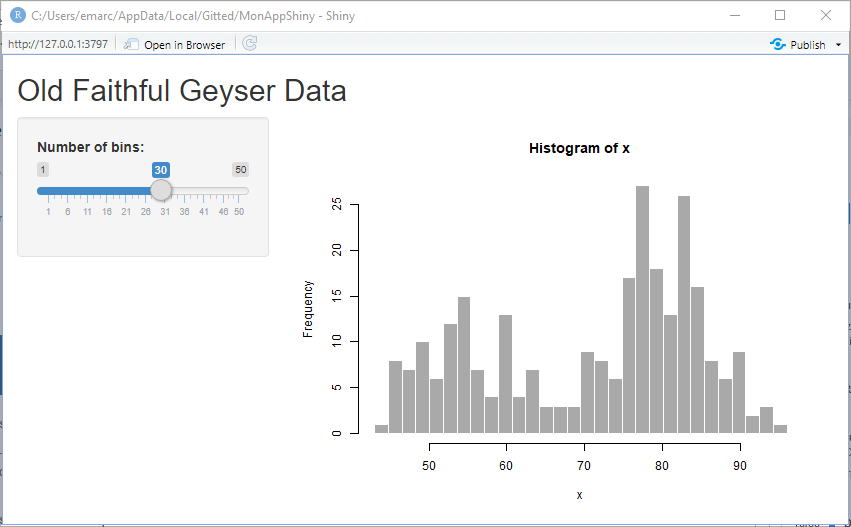
\includegraphics[width=0.8\linewidth]{images/shiny-geiser} 

}

\caption{Shiny Application \emph{Old Faithful Geyser Data}.}\label{fig:shiny-geiser}
\end{figure}

\normalsize

The correspondence between the displayed window (figure \ref{fig:shiny-geiser}) and the \texttt{ui()} function code is easy to see:

\begin{itemize}
\tightlist
\item
  The title of the application is displayed by the \texttt{titlePanel()} function.
\item
  The slider that sets the number of bars in the histogram is created by \texttt{sliderInput()}.
\item
  The \texttt{sidebarLayout()} function sets the layout of the page elements, \texttt{sidebarPanel} for the input controls and \texttt{mainPanel()} for the result display.
\end{itemize}

The result is displayed by the \texttt{plotOutput()} function whose argument is the name of an element of \texttt{output}, the variable filled by the \texttt{server()} function.

Any modification of an element of the interface, precisely of an element displayed by a function whose name ends with \texttt{Input()} (there are some for all types of inputs, for example \texttt{textInput()}) of \textbf{Shiny} causes \texttt{server()} to be executed and the elements of \texttt{output} to be updated.

\section{More elaborate application}\label{more-elaborate-application}

\subsection{Working method}\label{working-method}

An application is created by choosing:

\begin{itemize}
\tightlist
\item
  A window layout.
\item
  The controls for entering parameters (\emph{intput}).
\item
  The controls for displaying the results (\emph{output}).
\end{itemize}

The code to process the inputs and produce the outputs is then written to \texttt{server()}.

The RStudio tutorial\footnote{\url{https://shiny.rstudio.com/tutorial/}} is very detailed and should be used to go further.

\subsection{Example}\label{example}

This simple application uses the \textbf{scholar} package to query Google Scholar and get the bibliometric data of an author from his or her identifier.

The \texttt{app.R} file contains all the code and is built incrementally here.
The full application, with graphical output in addition to its simplified version presented here is available on GitHub\footnote{\url{https://github.com/EricMarcon/bibliometrics}}.

The beginning of the code consists of preparing the application to run by loading the necessary packages:

\scriptsize

\begin{Shaded}
\begin{Highlighting}[]
\CommentTok{\# Prepare the application \#\#\#\#}

\CommentTok{\# Load packages}
\FunctionTok{library}\NormalTok{(}\StringTok{"shiny"}\NormalTok{)}
\FunctionTok{library}\NormalTok{(}\StringTok{"tidyverse"}\NormalTok{)}
\end{Highlighting}
\end{Shaded}

\normalsize

The code of the complete application includes a function to install the missing packages, to be executed only when the application is executed on a workstation (on a server, the management of packages is not the responsibility of the application).

The user interface is as follows:

\scriptsize

\begin{Shaded}
\begin{Highlighting}[]
\CommentTok{\# UI \#\#\#\#}
\NormalTok{ui }\OtherTok{\textless{}{-}} \FunctionTok{fluidPage}\NormalTok{(}
  \CommentTok{\# Application title}
  \FunctionTok{titlePanel}\NormalTok{(}\StringTok{"Bibliometrics"}\NormalTok{),}
  
  \FunctionTok{sidebarLayout}\NormalTok{(}
    \FunctionTok{sidebarPanel}\NormalTok{(}
      \FunctionTok{helpText}\NormalTok{(}\StringTok{"Enter the Google Scholar ID of an author."}\NormalTok{),}
      \FunctionTok{textInput}\NormalTok{(}\StringTok{"AuthorID"}\NormalTok{, }\StringTok{"Google Scholar ID"}\NormalTok{, }\StringTok{"4iLBmbUAAAAJ"}\NormalTok{),}
      \CommentTok{\# End of input}
      \FunctionTok{br}\NormalTok{(),}
      \CommentTok{\# Display author\textquotesingle{}s name and h}
      \FunctionTok{uiOutput}\NormalTok{(}\StringTok{"name"}\NormalTok{),}
      \FunctionTok{uiOutput}\NormalTok{(}\StringTok{"h"}\NormalTok{)}
\NormalTok{    ),}
    \CommentTok{\# Show plots in the main panel}
    \FunctionTok{mainPanel}\NormalTok{(}
      \FunctionTok{plotOutput}\NormalTok{(}\StringTok{"network"}\NormalTok{),}
      \FunctionTok{plotOutput}\NormalTok{(}\StringTok{"citations"}\NormalTok{)}
\NormalTok{    )}
\NormalTok{  )}
\NormalTok{)}
\end{Highlighting}
\end{Shaded}

\normalsize

The application window is fluid, i.e.~it reorganizes itself when its size changes, and is composed of a side panel (for text input and display) and a main panel, for displaying graphics.

The elements of the side panel are:

\begin{itemize}
\tightlist
\item
  A help text: \texttt{helpText()}.
\item
  A text input field, \texttt{textInput()}, whose arguments are the name, the displayed text, and the default value (an author ID).
\item
  A line break: \texttt{br()}.
\item
  HTML output controls: \texttt{uiOutput()}, whose single argument is the name.
\end{itemize}

The main panel contains two graphical output controls, \texttt{plotOutput()} whose argument is also the name.

The code to execute to process the inputs and produce the outputs is in the \texttt{server()} function.

\scriptsize

\begin{Shaded}
\begin{Highlighting}[]
\CommentTok{\# Server logic \#\#\#\#}
\NormalTok{server }\OtherTok{\textless{}{-}} \ControlFlowTok{function}\NormalTok{(input, output) \{}
  \CommentTok{\# Run the get\_profile function only once \#\#\#\#}
  \CommentTok{\# Store the author profile}
\NormalTok{  AuthorProfile }\OtherTok{\textless{}{-}} \FunctionTok{reactiveVal}\NormalTok{()}
  \CommentTok{\# Update it when input$AuthorID is changed}
  \FunctionTok{observeEvent}\NormalTok{(}
\NormalTok{    input}\SpecialCharTok{$}\NormalTok{AuthorID, }
    \FunctionTok{AuthorProfile}\NormalTok{(}\FunctionTok{get\_profile}\NormalTok{(input}\SpecialCharTok{$}\NormalTok{AuthorID))}
\NormalTok{  )}
  
  \CommentTok{\# Output \#\#\#\#}
\NormalTok{  output}\SpecialCharTok{$}\NormalTok{name }\OtherTok{\textless{}{-}} \FunctionTok{renderUI}\NormalTok{(\{}
    \FunctionTok{h2}\NormalTok{(}\FunctionTok{AuthorProfile}\NormalTok{()}\SpecialCharTok{$}\NormalTok{name)}
\NormalTok{  \})}
  
\NormalTok{  output}\SpecialCharTok{$}\NormalTok{h }\OtherTok{\textless{}{-}} \FunctionTok{renderUI}\NormalTok{(\{}
    \FunctionTok{a}\NormalTok{(}\AttributeTok{href =} \FunctionTok{paste0}\NormalTok{(}
      \StringTok{"https://scholar.google.com/citations?user="}\NormalTok{, }
\NormalTok{      input}\SpecialCharTok{$}\NormalTok{AuthorID),}
      \FunctionTok{paste}\NormalTok{(}\StringTok{"h index:"}\NormalTok{, }\FunctionTok{AuthorProfile}\NormalTok{()}\SpecialCharTok{$}\NormalTok{h\_index),}
      \AttributeTok{target =} \StringTok{"\_blank"}
\NormalTok{    )}
\NormalTok{  \})}
  
\NormalTok{  output}\SpecialCharTok{$}\NormalTok{citations }\OtherTok{\textless{}{-}} \FunctionTok{renderPlot}\NormalTok{(\{}
    \FunctionTok{get\_citation\_history}\NormalTok{(input}\SpecialCharTok{$}\NormalTok{AuthorID)  }\SpecialCharTok{\%\textgreater{}\%}
      \FunctionTok{ggplot}\NormalTok{(}\FunctionTok{aes}\NormalTok{(year, cites)) }\SpecialCharTok{+}
      \FunctionTok{geom\_segment}\NormalTok{(}\FunctionTok{aes}\NormalTok{(}\AttributeTok{xend =}\NormalTok{ year, }\AttributeTok{yend =} \DecValTok{0}\NormalTok{), }\AttributeTok{size =} \DecValTok{1}\NormalTok{, }\AttributeTok{color =} \StringTok{\textquotesingle{}darkgrey\textquotesingle{}}\NormalTok{) }\SpecialCharTok{+}
      \FunctionTok{geom\_point}\NormalTok{(}\AttributeTok{size =} \DecValTok{3}\NormalTok{, }\AttributeTok{color =} \StringTok{"firebrick"}\NormalTok{) }\SpecialCharTok{+}
      \FunctionTok{labs}\NormalTok{(}
        \AttributeTok{title =} \StringTok{"Citations per year"}\NormalTok{,}
        \AttributeTok{caption =} \StringTok{"Source: Google Scholar"}
\NormalTok{      )}
\NormalTok{  \})}
  
\NormalTok{  output}\SpecialCharTok{$}\NormalTok{network }\OtherTok{\textless{}{-}} \FunctionTok{renderPlot}\NormalTok{(\{}
    \FunctionTok{ggplot}\NormalTok{() }\SpecialCharTok{+} \FunctionTok{geom\_blank}\NormalTok{()}
\NormalTok{  \})}
\NormalTok{\}}
\end{Highlighting}
\end{Shaded}

\normalsize

The information needed for the output fields \texttt{\$name} and \texttt{\$h} (author's name and h-index) is obtained by the \texttt{get\_profile()} function of the \textbf{scholar} package.
This function queries the author's Google Scholar web page and extracts the values from the result: this is a heavy processing, which is better executed only once rather than twice, in the \texttt{renderUI()} functions in charge of computing the values of \texttt{output\$h} and \texttt{output\$name}.

The simplest code to do this would be as follows:

\scriptsize

\begin{Shaded}
\begin{Highlighting}[]
  \CommentTok{\# Run the get\_profile function only once \#\#\#\#}
  \CommentTok{\# Store the author profile}
\NormalTok{  AuthorProfile }\OtherTok{\textless{}{-}} \FunctionTok{get\_profile}\NormalTok{(input}\SpecialCharTok{$}\NormalTok{AuthorID)}
\end{Highlighting}
\end{Shaded}

\normalsize

The difficulty with programming a Shiny application is that any computation referring to an input interface element must be \emph{reactive}.
If the latter code were executed, the following error message would appear:
\enquote{Operation not allowed without an active reactive context. (You tried to do something that can only be done from inside a reactive expression or observer.)}

In practice, the execution of the code is started by modifying an input control (here: \texttt{intput\$AuthorID}).
The code referring to one of these controls must be permanently waiting for a modification: it must therefore be placed in particular functions like \texttt{renderPlot()} in the \emph{Old Faithful Geyser Data} application or \texttt{renderUI()} here.
The following code would run without error:

\scriptsize

\begin{Shaded}
\begin{Highlighting}[]
  \CommentTok{\# Output \#\#\#\#}
\NormalTok{  output}\SpecialCharTok{$}\NormalTok{name }\OtherTok{\textless{}{-}} \FunctionTok{renderUI}\NormalTok{(\{}
\NormalTok{    AuthorProfile }\OtherTok{\textless{}{-}} \FunctionTok{get\_profile}\NormalTok{(input}\SpecialCharTok{$}\NormalTok{AuthorID)}
    \FunctionTok{h2}\NormalTok{(AuthorProfile}\SpecialCharTok{$}\NormalTok{name)}
\NormalTok{  \})}
\end{Highlighting}
\end{Shaded}

\normalsize

The call to the value of the \texttt{input\$AuthorID} control does occur in a reactive function (but \texttt{get\_profile()} would have to be used a second time in the calculation of \texttt{output\$h}, which we want to avoid).
The function \texttt{h2(AuthorProfile\$name)} produces HTML code, a level 2 title paragraph whose value is passed as an argument.

All functions whose names begin with \texttt{render} in the \textbf{shiny} package are reactive, and each is intended to produce a different type of output, for example text (\texttt{renderText()}) or HTML code (\texttt{renderUI()}).

If code is needed to compute variables common to several output controls (\texttt{output\$name} and \texttt{output\$h}), it must itself be responsive.
Two functions are very useful:

\begin{itemize}
\tightlist
\item
  \texttt{observeEvent()} watches for changes in an input control and executes code when they occur.
\item
  \texttt{reactiveVal()} allows you to define a reactive variable, which will be modified by the \texttt{observeEvent()} code and will in turn cause other reactive functions that use its value to execute.
\end{itemize}

So the optimal code creates a reactive variable to store the result of the Google Scholar query in:

\scriptsize

\begin{Shaded}
\begin{Highlighting}[]
  \CommentTok{\# Store the author profile}
\NormalTok{  AuthorProfile }\OtherTok{\textless{}{-}} \FunctionTok{reactiveVal}\NormalTok{()}
\end{Highlighting}
\end{Shaded}

\normalsize

The reactive variable is empty at this point.
Its use is then that of a function: \texttt{AuthorProfile(x)} assigns it the value \texttt{x} and \texttt{AuthorProfile()}, without arguments, returns its value.
The \texttt{observeEvent()} function is triggered when \texttt{input\$AuthorID} is modified and executes the code passed as the second argument, in this case the update of \texttt{AuthorProfile}.

\scriptsize

\begin{Shaded}
\begin{Highlighting}[]
  \CommentTok{\# Update it when input$AuthorID is changed}
  \FunctionTok{observeEvent}\NormalTok{(input}\SpecialCharTok{$}\NormalTok{AuthorID, }\FunctionTok{AuthorProfile}\NormalTok{(}\FunctionTok{get\_profile}\NormalTok{(input}\SpecialCharTok{$}\NormalTok{AuthorID)))}
\end{Highlighting}
\end{Shaded}

\normalsize

Finally, the \texttt{renderUI()} functions that provide output control values use the value of \texttt{AuthorProfile}:

\scriptsize

\begin{Shaded}
\begin{Highlighting}[]
  \CommentTok{\# Output \#\#\#\#}
\NormalTok{  output}\SpecialCharTok{$}\NormalTok{name }\OtherTok{\textless{}{-}} \FunctionTok{renderUI}\NormalTok{(\{}
     \FunctionTok{h2}\NormalTok{(}\FunctionTok{AuthorProfile}\NormalTok{()}\SpecialCharTok{$}\NormalTok{name)}
\NormalTok{  \})}
\end{Highlighting}
\end{Shaded}

\normalsize

Note the parentheses in \texttt{AuthorProfile()}, a reactive variable, as opposed to the \texttt{AuthorProfile\$name} syntax for a classic variable.

The value of \texttt{output\$h} is an internet link, \texttt{\textless{}a\ href=...} in HTML, written by the \texttt{a()} function of the \textbf{htmltools} package used by \texttt{renderUI()}.

\scriptsize

\begin{Shaded}
\begin{Highlighting}[]
\NormalTok{  output}\SpecialCharTok{$}\NormalTok{h }\OtherTok{\textless{}{-}} \FunctionTok{renderUI}\NormalTok{(\{}
    \FunctionTok{a}\NormalTok{(}\AttributeTok{href =} \FunctionTok{paste0}\NormalTok{(}
        \StringTok{"https://scholar.google.com/citations?user="}\NormalTok{, input}\SpecialCharTok{$}\NormalTok{AuthorID}
\NormalTok{      ),}
      \FunctionTok{paste}\NormalTok{(}\StringTok{"h index:"}\NormalTok{, }\FunctionTok{AuthorProfile}\NormalTok{()}\SpecialCharTok{$}\NormalTok{h\_index),}
      \AttributeTok{target =} \StringTok{"\_blank"}
\NormalTok{    )}
\NormalTok{  \})}
\end{Highlighting}
\end{Shaded}

\normalsize

The link is to the author's Google Scholar page.
The value displayed is its h index.
The argument \texttt{target\ =\ "\_blank"} indicates that the link should be opened in a new browser window.

The \texttt{output\$citations} graph is created by the \texttt{renderPlot()} reactive function.
The data provided by the \texttt{get\_citation\_history()} function of \textbf{scholar} (which queries the Google Scholar API) is processed by \texttt{ggplot()}.

Finally, the \texttt{output\$network} graph is an empty graph in this simplified version of the application.

The full application takes this code and adds error handling in case the author code does not exist on Google Scholar and the co-author network graph.

\section{Hosting}\label{sec:hebergement-shiny}

A Shiny application is not necessarily hosted by a web server: it can be run on users' workstations if they have R.

For a wider use, a dedicated server is necessary.
Shinyapps.io\footnote{\url{https://www.shinyapps.io/}} is a service from RStudio that allows to host 5 Shiny applications for free with a maximum uptime of 5 hours per month.

First of all, you have to open an account on the site, preferably with your GitHub identifiers.
To allow the management of online applications directly from RStudio, you must then install the \textbf{rsconnect} package and set it up:

\scriptsize

\begin{Shaded}
\begin{Highlighting}[]
\NormalTok{rsconnect}\SpecialCharTok{::}\FunctionTok{setAccountInfo}\NormalTok{(}
  \AttributeTok{name=}\StringTok{\textquotesingle{}firstname.name\textquotesingle{}}\NormalTok{,}
    \AttributeTok{token=}\StringTok{\textquotesingle{}xxx\textquotesingle{}}\NormalTok{,}
    \AttributeTok{secret=}\StringTok{\textquotesingle{}\textless{}SECRET\textgreater{}\textquotesingle{}}
\NormalTok{)}
\end{Highlighting}
\end{Shaded}

\normalsize

The exact code, along with the username and token to use, are displayed on the Shinyapps.io homepage: click on \enquote{Show Secret}, copy the code and paste it into the RStudio console to run it.
A \enquote{Publish} button is available just to the right of the \enquote{Run App} button.
Click on it and validate the publication (figure \ref{fig:shiny-publish}).



\scriptsize

\begin{figure}

{\centering 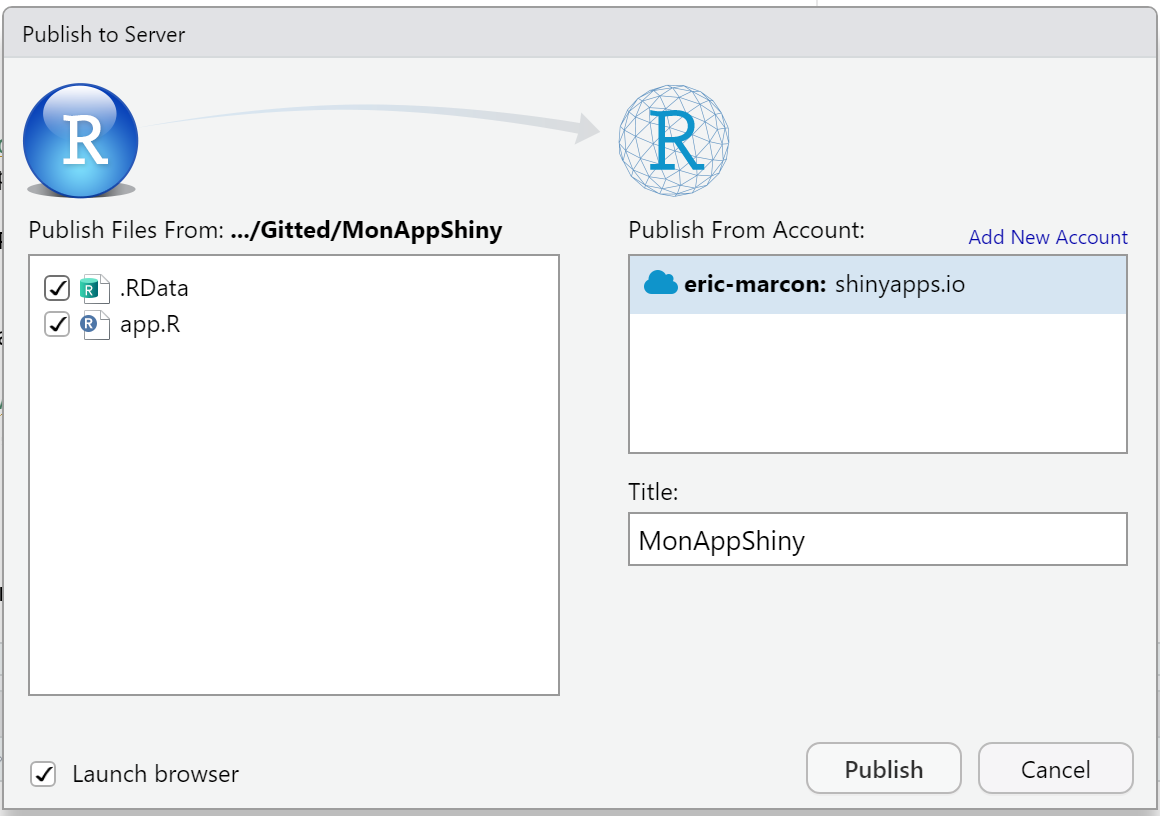
\includegraphics[width=0.8\linewidth]{images/shiny-publish} 

}

\caption{Publication of the Shiny application on Shinyapps.io.}\label{fig:shiny-publish}
\end{figure}

\normalsize

The application is now available at \url{https://firstname-lastname.shinyapps.io/MyShinyApp/}

The \enquote{Bibliometrics} application does not work on Shinyapps.io because the way the \textbf{Scholar} package queries Google Scholar is not supported.
Most Shiny applications work without difficulty, as long as they don't require complex networking features.

\chapter{Teaching with R}\label{chap-enseigner}

\toc{1}

R, RStudio and GitHub provide tools for teaching.

The \textbf{learnr} package allows you to make interactive tutorials.

We will also see how to use \emph{GitHub Classrooms} which allow to distribute to a class (a list of students with a GitHub account) a repository model (a draft of an R project) that each student will have to develop and publish.
The classroom tools allow to evaluate the work done quite easily.

\section{learnr}\label{learnr}

\textbf{learnr} allows you to make code snippets of any document produced by R Markdown in HTML interactive, by transforming them into Shiny applications.
The documentation on the RStudio website\footnote{\url{https://rstudio.github.io/learnr/}} is very clear and will not be repeated here: we will only see how to start and how to distribute the tutorials.

\subsection{First tutorial}\label{first-tutorial}

With the menu \enquote{File \textgreater{} New File \textgreater{} RMarkdown\ldots{}} create a new document from an \enquote{Interactive Tutorial} template.
The wizard creates a folder with the chosen name, to be transformed into an R project and put under source control, as for all documents seen previously (see section \ref{sec:memo}).

To run the tutorial, click on the \enquote{Run Document} button, which is in the usual place of the \enquote{Knit} button.

Tutorials can include exercises, which are code snippets with the \texttt{exercise=TRUE} option.
These exercises are displayed as a window of code that can be edited and executed by the user.
Hints can be given\footnote{\url{https://rstudio.github.io/learnr/exercises.html\#Hints_and_Solutions}}, a button added to display the solution, a time limit can be set\footnote{\url{https://rstudio.github.io/learnr/exercises.html\#Time_Limits}}, and both the code and its result can be compared to an expected value\footnote{\url{https://rstudio.github.io/learnr/exercises.html\#Exercise_Checking}}.

Quizzes\footnote{\url{https://rstudio.github.io/learnr/questions.html}} can be added, in the form of multiple or single choice quizzes.

The user's progress in the tutorial (code entered, answers to questions\ldots) is saved by \textbf{learnr} on the workstation.
A tutorial can be stopped and resumed without loss of data.
On the other hand, there is no easy way to recover this data for an evaluation by the trainer for example.

\subsection{Sharing}\label{sharing}

Tutorials can be distributed by copying the files or by telling users to clone the GitHub projects that contain them.

They can also be hosted on Shinyapps.io (see section \ref{sec:hebergement-shiny}).

Last, they can be included in a package\footnote{\url{https://rstudio.github.io/learnr/publishing.html\#R_Package}}.

\section{GitHub Classrooms}\label{github-classrooms}

GitHub Classrooms allows to distribute to a student audience GitHub repositories to modify and control the result.
The applications are as well the learning of R as the production of documents, for a personal work or an exam for example.

\subsection{Registration}\label{registration}

To start using the tool, you need to open an account.
On the GitHub Classrooms website\footnote{\url{https://classroom.github.com/}}, click on \enquote{Sign in} and use your GitHub account to authenticate.

\subsection{Organizations}\label{organizations}

The next step is to create a GitHub organization.
A GitHub organization basically contains members (GitHub account holders) and repositories that can be accessed at \url{https://github.com/}/.

The simplest way to work is to create an organization per course, but other approaches are possible in structures that use the tool extensively.
The organization created for the example here is \enquote{Cours-R}\footnote{\url{https://github.com/Cours-R}}.

An email address is required (use the same as that of your GitHub account) and the organization must be declared as belonging to your personal account.

If the organization is not visible on the GitHub Classrooms page, click on \enquote{Grant us access}.

\subsection{New Classroom}\label{new-classroom}

A classroom is populated with students who will receive tasks to perform.

Click on \emph{New Classroom}.
Select the organization in charge of administering the classroom.

Enter the name of the classroom: a good practice is to prefix it with the name of the course and add the name of the session, for example \enquote{Cours-R-2020}.

Do not add collaborators (this will be possible later), and eventually enter the list of students (one name per line, also possible later).
The class is created.

All classrooms are visible from the GitHub Classrooms homepage\footnote{\url{https://classroom.github.com/classrooms}}.
Click on a name to open one.
The \enquote{Settings} button allows to change its name or to delete it.
The \enquote{TAs and Admins} button allows you to add collaborators, i.e.~other GitHub users who will be able to administer the classroom.

The \enquote{Students} button allows to add students.
The list of names is free, with no mandatory format.
Click on \enquote{Create Roster} to activate it.
The names must then be linked to GitHub accounts: this work can be done by the administrator or by the students themselves when they receive the first task to be done.
Each student must have an account on GitHub.

\subsection{Prepare a repository template}\label{prepare-a-repository-template}

A task is a GitHub repository to modify.
For example\footnote{\url{https://github.com/EricMarcon/Cours-R-Memo/settings}}, create a repository containing an R project with a Markdown file describing the work to be done and possibly some of the code needed to do it, the other files in the R Markdown template used and a data file.

Open the repository properties on GitHub and check the \emph{Template Repository} box to make it a template.

\subsubsection{Assign a task}\label{assign-a-task}

Open a classroom and click on \enquote{New Assignment}.

Enter an explicit title for the students, an optional deadline and choose \enquote{Individual Assignment}.

By default, the assignment name is used as a prefix for the students' submission names, but it can be replaced by a prefix of your choice.
When students turn in their work, all repositories for all tasks will be stored in the organization.

The repository created on each student's account can be private or public, depending on whether you want students to be able to see each other's work or not.
Give the administration right and make the site public if the students should be able to activate GitHub pages to present the results of their work.
Click on \enquote{Continue}.

Select the model repository (\emph{starter code}) then click on \enquote{Continue} then \enquote{Create Assignment}.

The new task is created.
It is associated with an invitation link that must be copied and sent to the students.
When they click on the link, they will reach a GitHub page that will allow them to associate their account with a name in the list (no control is possible: the first one connected can associate with any name).
They will then be able to create a new RStudio project from the GitHub repository automatically created by GitHub Classrooms, modify that project according to the work instructions and push it to GitHub.
The repository is on the account of the organization the class is connected to, and is suffixed with the student's GitHub ID.

\subsubsection{Controlling student work}\label{controlling-student-work}

It is possible to view each repository created by students from the assignment page on GitHub Classrooms.
If the assignment to be produced is a written document, have students place it in the repository's GitHub pages to read it directly online.

The GitHub Classrooms wizard\footnote{\url{https://classroom.github.com/assistant}} allows you to download all student repositories at once to correct them on your workstation.

\chapter{Conclusion}\label{chap-conclusion}

The R and RStudio work environment allows for the production of all types of documents with a single language.

The objective of reproducibility of results is achieved by integrating statistical processing and writing.
Collaborative work is allowed by the systematic use of source control and GitHub.
The presentation of results is ensured by GitHub pages and document templates covering most needs.

For breaks, R even provides some games in the \textbf{fun} package, including the famous Minesweeper:

\scriptsize

\begin{Shaded}
\begin{Highlighting}[]
\CommentTok{\# Install the package}
\FunctionTok{install.packages}\NormalTok{(}\StringTok{"fun"}\NormalTok{)}
\CommentTok{\# Open an X window and run}
\ControlFlowTok{if}\NormalTok{ (}\FunctionTok{interactive}\NormalTok{()) \{}
  \ControlFlowTok{if}\NormalTok{ (.Platform}\SpecialCharTok{$}\NormalTok{OS.type }\SpecialCharTok{==} \StringTok{"windows"}\NormalTok{) \{}
    \FunctionTok{x11}\NormalTok{() }
\NormalTok{  \} }\ControlFlowTok{else}\NormalTok{ \{ }
    \FunctionTok{x11}\NormalTok{(}\AttributeTok{type =} \StringTok{"Xlib"}\NormalTok{)}
\NormalTok{  \}}
\NormalTok{  fun}\SpecialCharTok{::}\FunctionTok{mine\_sweeper}\NormalTok{()}
\NormalTok{\}}
\end{Highlighting}
\end{Shaded}

\normalsize

This document does not aim to be exhaustive on the possibilities of R but rather to present a working method and simple ways to apply it quickly.
You can refer to the more detailed books and documentations cited in the text to go deeper into a particular point.

It is updated regularly as the available tools evolve.


% Bibliography
%%%%%%%%%%%%%%%%%%%%%%%%%%%%%%%%%%%%%%%%%%%%%%%%%%%%%%%%%%

\backmatter
\SmallMargins

\printbibliography
\onecolumn


% Tables (of tables, of figures)
%%%%%%%%%%%%%%%%%%%%%%%%%%%%%%%%%%%%%%%%%%%%%%%%%%%%%%%%%%


\cleardoublepage
\LargeMargins
\listoffigures


% After-body (LaTeX code inclusion)
%%%%%%%%%%%%%%%%%%%%%%%%%%%%%%%%%%%%%%%%%%%%%%%%%%%%%%%%%%




% Back cover
%%%%%%%%%%%%%%%%%%%%%%%%%%%%%%%%%%%%%%%%%%%%%%%%%%%%%%%%%%%

% Even page, small margins, no running head, no page number.
\evenpage
\SmallMargins
\thispagestyle{empty}

\begin{normalsize}

\begin{description}

\selectlanguage{english}
\item[Abstract]
This book proposes an organization of work around R and RStudio to, beyond statistics, write documents efficiently with R Markdown, in various formats (memos, scientific articles, student theses, books, slideshows), create websites and online R applications (Shiny), produce packages and use R for teaching.
\item[]
.
~\\

\end{description}

\end{normalsize}


\end{document}
